\documentclass[12pt,twoside]{book}
\usepackage{layout}
%\usepackage{makeidx}
\RequirePackage{verbatim}
%\RequirePackage{alltt}
\usepackage{ifpdf}
\usepackage{etoolbox}
\usepackage{multicol}

\newtoggle{solutions}
\toggletrue{solutions}
\togglefalse{solutions}

\ifpdf 
   \pdfcompresslevel=9
   \pdfoutput=1


   \usepackage[pdftex]{graphicx}
   \usepackage[pdftex]{geometry}
   \usepackage[pdftex]{color}
   \usepackage{hyperref}
   \hypersetup{
     pdftitle={Recitation Activities for the COMPASS program, Semester II},
     pdfsubject={ODE},
     pdfauthor={Kelly Black},
     pdfkeywords={classroom activities, calculus, physics},
     anchorcolor = {red},
     colorlinks = {true},
     %pdfpagemode={FullScreen}
   }
\else
   \usepackage{epsfig}
   \usepackage{color}
\fi

\usepackage{pgf}
\usepackage{pstricks} 
\usepackage{tikz}
\usetikzlibrary{shapes,arrows}


\pagestyle{myheadings}

%\setlength{\basicoddside}{\oddsidemargin}
%\setlength{\basicevenside}{\evensidemargin}
%\setlength{\basicwidth}{\textwidth}
%\setlength{\basictop}{\topmargin}
%\setlength{\basicheight}{\textheight}


\newcommand{\introduction}[1]{}

\font\tenit=cmti10
\makeatletter

\renewcommand{\@evenfoot}{\tenit University of Georgia Department of
  Mathematics\hfill}
\renewcommand{\@oddfoot}{\tenit \hfill Coordinated Math-Physics Program - \today}

\renewcommand{\section}{\@startsection
  {section}
  {1}
  {0em}
  {\baselineskip}
  {-1em}
  {\normalfont\normalsize\bfseries}}

\renewcommand{\subsection}{\@startsection
  {subsection}
  {2}
  {0em}
  {\baselineskip}
  {-1em}
  {\normalfont\normalsize\bfseries}}

\renewcommand{\subsubsection}{\@startsection
  {subsubsection}
  {2}
  {0em}
  {\baselineskip}
  {-2em}
  {\normalfont\normalsize\itshape}}

\makeatother


\newlength{\basicoddside}
\newlength{\basicevenside}
\newlength{\basicwidth}
\newlength{\basictop}
\newlength{\basicheight}

\newcommand{\activityParams}{
  %\setlength{\hoffset}{0in}
  %\setlength{\oddsidemargin}{-0.5in}
  %\setlength{\evensidemargin}{-0.5in}
  %\setlength{\textwidth}{7.5in}
  \setlength{\topmargin}{-0.5in}
  \setlength{\textheight}{9in}
}

\newcommand{\textParams}{
  \setlength{\oddsidemargin}{\basicoddside}
  \setlength{\evensidemargin}{\basicevenside}
  \setlength{\textwidth}{\basicwidth}
  \setlength{\topmargin}{\basictop}
  \setlength{\textheight}{\basicheight}
}


  \setlength{\oddsidemargin}{-0.25in}
  \setlength{\evensidemargin}{0.25in}
  \setlength{\textwidth}{6.25in}
  \setlength{\topmargin}{-0.5in}
  \setlength{\textheight}{9in}
  \setlength{\marginparwidth}{56pt}


\newcommand{\sideNote}[1]{\marginpar{\tenit \raggedright #1}}
\newcommand{\doNotPrint}[1]{}


\newtheorem{lemma}{Lemma}[subsection]
\newtheorem{theorem}{Theorem}[subsection]



\newcounter{activity}
\setcounter{activity}{1}

\newcommand{\actTitle}[1]{
  \cleardoublepage
  \activityParams
  \stepcounter{activity}
  \markboth
  {Name: \hspace*{2.5in} \hfil  Activity: \theactivity}
  {Name: \hspace*{2.5in} \hfil  Activity: \theactivity}
  \stepcounter{subsection}
  \addcontentsline{toc}{subsection}{
    \protect\numberline{\thesubsection}{#1}}
}

\newcounter{hw}
\setcounter{hw}{0}
\newcommand{\hwTitle}[1]{
  \cleardoublepage
  \activityParams
  \stepcounter{hw}
  \markboth
  {Name: \hspace*{2.5in} \hfil  Home Work: \thehw}
  {Name: \hspace*{2.5in} \hfil  Home Work: \thehw}
  \stepcounter{subsubsection}
  \addcontentsline{toc}{subsubsection}{
    \protect\numberline{\thesubsubsection}{#1}}
}

\newcommand{\preClass}[1]{
  \cleardoublepage
  \activityParams
  \markboth
  {Name: \hspace*{2in} \hfil Preclass Work - Finish Before Class Begins \hfil}
  {Name: \hspace*{2in} \hfil Preclass Work - Finish Before Class Begins \hfil}
  \stepcounter{subsubsection}
  \addcontentsline{toc}{subsubsection}{
    \protect\numberline{\thesubsubsection}{#1}}
}

\newcommand{\postClass}{
  \cleardoublepage
  \activityParams
  \markboth
  {Name: \hspace*{2in} \hfil Postclass Work - Finish After Class \hfil}
  {Name: \hspace*{2in} \hfil Postclass Work - Finish After Class \hfil}
%  \stepcounter{subsubsection}
%  \addcontentsline{toc}{subsubsection}{
%    \protect\numberline{\thesubsubsection}{#1}}
}


\newcounter{quiz}
\setcounter{quiz}{1}
\newcommand{\qzTitle}[1]{
  \cleardoublepage
  \activityParams
  \stepcounter{quiz}
  \markboth
  {Name: \hspace*{2.5in} \hfil  #1 Quiz: \thequiz}
  {Name: \hspace*{2.5in} \hfil  #1 Quiz: \thequiz}
  \stepcounter{subsubsection}
  \addcontentsline{toc}{subsubsection}{
    \protect\numberline{\thesubsubsection}{#1}}
}


\newcommand{\stateSummary}{\item State and summarize two ideas from today's
  class. 
  \vfill 
  \centerline{\textit{(Over)}}
  \clearpage }


\newcommand{\addTOC}[1]{
  \stepcounter{section}
  \addcontentsline{toc}{section}{
    \protect\numberline{\thesection}{#1}}
  }



\newenvironment{problem}
{\begin{list}
{\arabic{enumi}.}
{\usecounter{enumi}
\setlength{\rightmargin}{0pt}
%\setlength{\rightmargin}{-72pt}
\setlength{\parsep}{1em}
\setlength{\listparindent}{0pt}
}}
{\end{list}}

\newenvironment{subproblem}
{\begin{list}
{(\alph{enumii})}
{\usecounter{enumii}
\setlength{\rightmargin}{0pt}
\setlength{\parsep}{1em}
\setlength{\listparindent}{0pt}
}}
{\end{list}}

\newenvironment{multiEqn}
{\begin{eqnarray*} 
 \begin{array}{rclclclcl}}
{\end{array}
 \end{eqnarray*}}


\setcounter{activity}{0}


% %%%%%%%%%%%%%%%%%%%%%%%%%%%%%%%%%%%%%%%%%%%%%%%%%%%%%%%%%%%%%%%%%%%%%%%
% List of definitions that are used in the different pages for the
% notes

% %%%%%%%%%%%%%%%%%%%%%%%%%%%%%%%%%%%%%%%%%%%%%%%%%%%%%%%%%%%%%%%%%%%%%%%
% Basic definitions used throughout the notes

\newcommand{\change}[1]{\triangle #1}
\newcommand{\fortyFive}{\frac{\sqrt{2}}{2}}
\newcommand{\imag}{j}
\newcommand{\half}{\mbox{$\frac{1}{2}$}}
\newcommand{\deltat}{\mbox{$\triangle t$}}
\newcommand{\deltax}{\mbox{$\triangle x$}}
\newcommand{\deltay}{\mbox{$\triangle y$}}

\newcommand{\deriv}[2]{\frac{d}{d#2}#1}
\newcommand{\derivTwo}[2]{\frac{d^2}{d#2^2}#1}

\newcommand{\lp}{\left(}
\newcommand{\rp}{\right)}


% %%%%%%%%%%%%%%%%%%%%%%%%%%%%%%%%%%%%%%%%%%%%%%%%%%%%%%%%%%%%%%%%%%%%%%
% Basic linear algebra commands

\newcommand{\arrayTwo}[4]{
  \left[
  \begin{array}{rr}
    #1 & #2 \\
    #3 & #4
  \end{array}
  \right]
}

\newcommand{\vecTwo}[2]{
  \left[
  \begin{array}{r}
    #1 \\  #2
  \end{array}
  \right]
}

\newcommand{\vecFour}[4]{
  \left[
  \begin{array}{r}
    #1 \\  #2 \\ #3 \\ #4
  \end{array}
  \right]
}


\newcommand{\stateTwo}[2]{
  \begin{array}{rr}
    \mbox{\fontsize{6}{6}\selectfont $#1$} \\  \mbox{\fontsize{6}{6}\selectfont $#2$}
  \end{array}
}


\newcommand{\arrayThree}[9]{
  \left[
    \begin{array}{rrr}
      #1 & #2 & #3 \\
      #4 & #5 & #6 \\
      #7 & #8 & #9
    \end{array}
  \right]
}

\newcommand{\startRowOps}{
  \left[
    \begin{array}{rrr|r}
}

\newcommand{\oneRowOps}[4] {
      #1 & #2 & #3 & #4 \\
}

\newcommand{\stopRowOps}{
    \end{array}
  \right]
}


\newcommand{\vecThree}[3]{
  \left[
  \begin{array}{r}
    #1 \\  #2 \\ #3
  \end{array}
  \right]
}


\newcommand{\stateThree}[3]{
  \begin{array}{r}
    \mbox{\fontsize{6}{6}\selectfont $#1$} \\  
    \mbox{\fontsize{6}{6}\selectfont $#2$} \\ 
    \mbox{\fontsize{6}{6}\selectfont $#3$}
  \end{array}
}





\newcommand{\detTwo}[4]{
  \left|
  \begin{array}{rr}
    #1 & #2 \\
    #3 & #4
  \end{array}
  \right|
}



\newcommand{\detThree}[9]{
  \left|
    \begin{array}{rrr}
      #1 & #2 & #3 \\
      #4 & #5 & #6 \\
      #7 & #8 & #9
    \end{array}
  \right|
}




\newcommand{\startRowFour}{
  \left[
    \begin{array}{rrrr}
}

\newcommand{\oneRowFour}[4] {
      #1 & #2 & #3 & #4 \\
}




\newcommand{\startRowOpsTwo}{
  \left[
    \begin{array}{rr|rr}
}

\newcommand{\oneRowOpsTwo}[4] {
      #1 & #2 & #3 & #4 \\
}


\newcommand{\startRowOpsThree}{
  \left[
    \begin{array}{rrr|rrr}
}

\newcommand{\oneRowOpsThree}[6] {
      #1 & #2 & #3 & #4 & #5 & #6 \\
}





%%% Local Variables: 
%%% mode: latex
%%% TeX-master: t
%%% End: 


\begin{document}


\title{Classroom Activities \\ 
  Semester II \\
  Coordinated Math-Physics Program
  \iftoggle{solutions}{%
    \\\textit{Solution Manual}
  }
}
\author{Kelly Black\\University of Georgia\\Department of Mathematics}

\maketitle

\noindent
Copyright (C)  2015-2016 Kelly Black

\noindent
Permission is granted to copy, distribute and/or modify this document
under the terms of the GNU Free Documentation License, Version 1.3
or any later version published by the Free Software Foundation;
with no Invariant Sections, no Front-Cover Texts, and no Back-Cover Texts.
A copy of the license is included in the section entitled "GNU
Free Documentation License".



\tableofcontents

%\clearpage

\chapter{Preliminaries}


\newcommand{\mlc}[1] {\texttt{>> #1 }}
\newcommand{\ttt}[1]{\texttt{#1}}

\section{MATLAB} 

\textbf{Note:} For a general introduction to MATLAB see \textit{The
  MATLAB User's Guide, Reference Manual}, or other \textit{MATLAB}
manuals.  You can buy the student edition of MATLAB.  It comes with a
good manual. \index{MATLAB}\\


If you are using MATLAB in other classes, you may consider buying the 
\textbf{MATLAB Guide} by Desmond J. Higham and Nicholas J. Higham, published
by Siam.\\ 
  

\subsection{Basic operations} Addition, subtraction, and arrays.  The 
command 'Press Enter' is abbreviated by ENTER. \\
\vspace{1in}


\begin{tabular}{lll} 
  \ttt{>>} 3+5     &ENTER   &Add two numbers and display results. \\ 
  \ttt{>>} 4-6     &ENTER   &Subtract two numbers and display results. \\ 
  \ttt{>>} 4-6;    &ENTER   &Subtract two numbers and do NOT
  display results.\\
  \ttt{>>} a = 12/5; &ENTER   &Divide and store result in variable 'a'.\\
  \ttt{>>} a        &ENTER  &Display content of variable 'a'. \\
  \ttt{>>} 1:2:11   &ENTER  &Generate a list of values. \\
  \ttt{>>} b=1:0.1:2 &ENTER & Fill an array with values from 1 to
  2 in increments of 0.1.\\
  \ttt{>>} b          &ENTER & Display content of 'b'. \\
  \ttt{>>} who      &ENTER  &List current variables. \\
  \ttt{>>} whos     &ENTER  &List current variables and their size.\\
  \ttt{>>} d = 5:1:15 &ENTER &Fill array 'd'. \\
  \ttt{>>} b + d     &ENTER &Add two arrays. \\
  \ttt{>>} b .* d    &ENTER & Multiply two arrays component wise. \\
  \ttt{>>} b * d     &ENTER & \\ 
  \ttt{>>} g = [1 2; 3 4; 5 6] &ENTER &Define a two dimensional array. \\
  \ttt{>>} g2 = 2*g  &ENTER & Multiply array by a constant. \\
\end{tabular}

\subsection{Creating a function plot} ~ \\
\begin{tabular}{lll}
  \ttt{>>} \verb!x = -5:0.1:5;!  &ENTER  &Set up the independent variable. \\
  \ttt{>>} y = \verb!x.^2!; &ENTER  & Compute dependent variable or
  y-values . \\ 
  \ttt{>>} z = \verb!(1/8)*x.^3!;      &ENTER  & Compute values for
  a second function. \\ 
  \ttt{>>} plot(x,y);     &ENTER  & Plot x versus y. \\
  \ttt{>>} hold on;      &ENTER &Hold current graph . \\
  \ttt{>>} plot(x,z,'r'); &ENTER &Plot graph of 'z', in red, on same
  axis as 'y', \\
  \ttt{>>} title('y, z, versus x'); & ENTER & Set the title for the
  plot. \\
  \ttt{>>} hold;         &ENTER &Release current plot.  Next plot
  property is 'replace'. \\ 
\end{tabular}

\subsection{Sums and loops} ~ \\
\begin{tabular}{lll}
  \ttt{>>} u = [ 1 2 3 4 5]  &ENTER &Define the row vector 'u'. \\
  \ttt{>>} v = [ 6 7 8 9 10 ]' &ENTER &Define the column vector 'v'.\\
  \ttt{>>} w = (1:0.2:20)' &ENTER & Define the column vector 'w'. \\
  \ttt{>>} whos     &ENTER &Check the dimensions of the vectors. \\
  \ttt{>>} help sum &ENTER &  Example:  Get help with the
  SUM command. \\ 
  \ttt{>>} sum(v,1) &ENTER &Add values of  vector 'v'.\\
  \ttt{>>} sum(u,1) &ENTER &Observe results. \\ 
  \ttt{>>} sum(u,2) &ENTER & Add values of vector 'v'. \\
  \ttt{>>} \%  This is a comment line  &ENTER & \\  
  \ttt{>>} \%  Next we will try a for loop. &ENTER & \\
  \ttt{>>} clear x; &ENTER &  clear x-variable.  \\      
  \ttt{>>} n = 10;  &ENTER &Set up loop limit. \\
  \ttt{>>} for i = 1:n, x(i) = i+1, end  &ENTER  & \\
  \ttt{>>} x   &ENTER &Display content of vector 'x'. \\
  \ttt{>>} clear &ENTER & Clear all variables. \\
\end{tabular}

\subsection{Editing and running M-files} You can do many useful computations
working entirely at the MATLAB command line, but soon you will find it helpful
to save a list of commands to an M-file.  M-file are the equivalents of programs
functions, subroutines, and procedures in other programming languages.

An M-file is a text file that has a \textbf{.m} filename extension and contains 
MATLAB commands.

There are two types:
\begin{itemize}
  \item{\textbf{Script M-files}} (or command files) have no input or output
  arguments and operate on variables in the workspace.  A script enables you to
  store a sequence of commands that are to be used repeatedly or will be needed
  at some future time.
  
  \item{\textbf{Function M-files}} contain a function definition line and can
  accept input arguments and return output arguments and their internal
  variables are local to the function (unless declared global).
\end{itemize}

\begin{enumerate}
  \item To create an M-file click on the "new file" icon \textbf{or}\\
  $\rightarrow$ Select File
  
  \hspace{.2in}$\rightarrow$  Select New 
  
  \hspace{.4in}$\rightarrow$  Select M-file\\
  A text edit window will open.
  
  \item Enter the following MATLAB commands to create a MATLAB script.\\
  \verb!% Plot the function y=x^2.!\\
  \verb!% This is my first M-file experience!\\
  \ttt{x=-5:0.001:5;}\\
  \verb!y=x.^2;!\\
  \ttt{plot (x,y)}
  
  \item Save the M-file to the E: drive in the "Calculus" folder as test1.m.
  
  If this is the first time you are running MATLAB, you may need to create the
  folder "Calculus."
  
  When MATLAB opens, the default directory is S:$\backslash$NetApps$\backslash$ 
  MATLAB$\backslash$bin$\backslash$win32.  To change the directory click on the
  icon to the right of the displayed directory name.  The "Browse for Folder"
  window will open.\\
  $\rightarrow$ Click on E: to select the E: drive.\\
  $\rightarrow$ Click on the "New Folder" icon and type the word "Calculus" to
  name the new folder.\\
  $\rightarrow$ Now save your M-file to the folder "Calculus."
  
  \item To execute the MATLAB script click on the "Save and Run" or "Run" icon. 
  The first time you select the "Run" command the MATLAB Editor window will open
  containing the following information:
  
  File E:$\backslash$Calculus$\backslash$test1.m is not found in the current
  or on the MATLAB path.\\ 
  To run this file, select one of the following:
  \begin{itemize}
    \item Change MATLAB current directory
    \item Add directory to the top of the MATLAB path
    \item Add directory to the bottom of the MATLAB path.
  \end{itemize}
  Select "Add directory to the top of the MATLAB path" and click on OK.
  
  MATLAB will then execute the script.  What do you observe?
  
  \item Next create a function called f1.m that will generate the points to plot
  the function $f(x)=e^{(-x/3)}\sin(2x)$ using M-file.
  
  Open a new M-file and type the following commands:
  \begin{verbatim}
    function y=f1(x)
    % y=f1(x) : This is my second M-file experience
    y=exp(-x/3).*sin(2*x);
  \end{verbatim}
  Save the file as f1.m to the Calculus folder on the E: drive.
  
  To execute the function we first need to define $x$.  Return to the command
  window and define $x$  and execute the function as follow:\\
  \begin{verbatim}
    >> x1=-5:0.01:5;
    >> y1=f1(x1); % execute function
    >> plot(x1,y1)
  \end{verbatim}
  
  MATLAB has a help command that can be invoked.  The MATLAB help function outputs
  all the comment lines before the first blank line in an M-file.  Enter\\
  \mlc{help f1}\\
  The last example was a function with a single input and one output.  A function
  can include more than one input or output.  The next example will construct a
  function with one input and two outputs.
  
  Open a new M-file and type the following commands:
  \begin{verbatim}
    function [y,z]=f2(x)
    %[y,z]=f2(x)  My third M-file.
    y=exp(-x/3).*sin(2*x);
    z=exp(-x/3).*cos(2*x);
  \end{verbatim}
  Save the file as f2.m to the Calculus folder on the E: drive.
  
  To execute this function and to plot the output type the following commands in 
  the command window:\\
  \mlc{[y1,z1]=f2(x1);}\\
  \mlc{plot(x1,[y1,z1])}\\
  
  \item Our next example is a more complex M-file script.  Functions are like
  subroutines in that they have their own internal variables and communicate
  with the command window and the workspace through their inputs and outputs. 
  Scripts, on the other hand, are simply sequences of commands which operate on
  the variables in the workspace.  Any variable created in a script is placed in
  the workspace.  For that reason it is good practice to clear any variables
  which are no longer needed.  Scripts do not use inputs or create outputs and
  will give an error if you ask for it.  (Functions need not have outputs
  however.)  We will call the script f2\_plot.m.
  
  Open a new M-file and type the following commands:
  \begin{verbatim}
    % f2_plot	(Note: Not a "function" so first line can be a comment)
    % Script to plot output of function f2    
    [u,v] = f2(x1);
    figure(1)
    subplot(2,1,1); plot(x1,[u,v]);
    title('u, v versus x');
    xlabel('x1');
    ylabel('Feet');
    w = u.*v;
    z = u.^2+v.^2;
    subplot(2,1,2); plot(x1,[w,z]);
    title('w, z versus x');
    xlabel('x1');
    ylabel('Sq. Feet');
    clear u v w z
  \end{verbatim}
  Save the M-file as f2\_plot.m to the Calculus folder on the E: drive.
  
  To execute the M-file script either click on the "Run" icon or type f2\_plot
  at the \ttt{>>} command prompt in the command window.
  
  What do you observe?  What effect does the subplot command have?
  \vspace{.25in}
  
  \item We will do one more example of a function.  This function will create a
  sequence of numbers, called the Fibonacci sequence.  It will have one input
  and one output and use a "for" loop to generate the sequence.
  \clearpage
  Open a new M-file type the following commands including the comments:
  \begin{verbatim}
    function y=fibonacci(n)
    % y=fibonacci(n)
    % Populate the vector y with the first n terms of the Fibonacci sequence,
    % using a "for" loop.
    % The sequence is named after the Italian mathematician Leonardo Pisano,
    % nicknamed Leonardo Fibonacci, who lived about 1175-1250 AD.
    % After the second term, the Fibonacci sequence is generated by adding the
    two previous terms to generate the current term.
    y(1)=1;
    y(2)=1;
    for i=3:n
        y(i)=y(i-1)+y(i-2);
    end
  \end{verbatim}
  Save the M-file as fibonacci.m in the Calculus folder on the E: drive.
  
  To display the comments at the beginning of the fibonacci.m file and to
  execute it, type the following commands in the command window:
  \begin{verbatim}
  >>help fibonacci
  >>n=5
  >>y1=fibonacci(n)
  \end{verbatim}
  
  If you would like to plot the sequence type the following commands in the
  command window:
  \begin{verbatim}
  >>n=1:1:12;
  >>n1=12;
  >>y=fibonacci(n1);
  >>plot(n,y,'*')
  \end{verbatim}
  What do you observe?
  
     
\end{enumerate}



\section{Assignment Guidelines}


\subsection{Home Work} \index{Home Work}
All work that is handed in for a grade must be neat. Any work that
cannot be easily read will not be graded. Every home work assignment
must have your name at the top of every page and all sheets must be
stapled together. Assignments that are not stapled will have points
deducted.

The front page must have your name written on it. The front page must
also have three other items. First, the current assignment should be
written. Secondly, it should have the times that you planned in
advance to work on the homework. Third, it should have the times that
you did the actual work.

Each page must be one column. Your solutions to the home work problems
should be written out one after the other and not on the same line.
For example, after completing a problem the next problem should appear
directly below the previous problem. Once you reach the bottom of the
page you must move on to the next page and not start over in a second
column on the current page.

A front page should look like the following: \\
\begin{center}
\fbox{
\begin{minipage}[h]{4in}
Stuart Dent \\
Page 32 1-5 odd, 27, 29, and 35. \\
Page 107 21-31 odd, 35a, and 42. 

\vspace{2em}

Original times: Tuesday 5-6pm, Wednesday 4:30-5:30, and Thursday
6-7pm.

\vspace{2em}

Actual times: Thursday 8pm to Friday 2am.

\vspace{2em}

Page 32: \\
1) $\frac{d}{dt} t^2 = 2t$.

3) $\frac{d}{dt} \left( \sqrt{t} + t \right)  = 
    \frac{1}{2} t^{-\frac{1}{2}} + 1$

$\vdots$

\end{minipage}}
\end{center}

\subsection{Group Work} \index{Group Work}
For many of the assignments in this class you will be required to work
in small groups.  Please keep in mind the following guidelines when
taking part in group work: \index{group work}
\begin{enumerate}
\item Cooperate with each other. Work together and find a solution to
  the problem together.

\item Make sure that everyone understands each answer before the group
  moves on to the next question.

\item Listen carefully to each other and try, whenever possible, to
  build upon their ideas.

\item Share in the leadership of the group.  You may wish to assign
  different roles, i.e. moderator, recorder, etc., to different
  individuals.
  
\item Make sure that everyone participates and that no one dominates.
  If you see someone in the group who is lost, urge him or her to ask
  questions, or ask a simple question yourself to bring others into
  the discussion.

\item Ask questions when you don't understand something.

\item Do not be critical of other people's \textbf{questions}.
\end{enumerate}



\subsection{Projects} \index{Projects}
Formal projects will be assigned in this class. You will have between
one and two weeks to complete each project. You will either present
the project in a presentation in front of the class or turn in a
written report. 

Before the due date of the project you must meet with your professor
at least twice. All members of your group should be present at the
meeting. Meetings should be scheduled at the beginning of project work
on the Friday that projects are handed out.  \index{meeting} Your
group needs to meet for at least an hour before this meeting. The
total length of the meeting is 30 minutes. After 30 minutes the
meeting is concluded.

\subsubsection {Rewrites}
Written submissions can be rewritten and resubmitted within a week
after they are turned back to you.  \index{written projects} You may be
able to increase your grade significantly with a modicum of extra work
by using our suggestions to improve the quality of the presentation.


\subsubsection{Outline for the Written  or Oral Presentation}

The formal write up for this lab should be about five pages long and
should be typed. \index{written projects} But we will be more
concerned about whether or not the key questions are answered rather
than the length of the write up.  The text should be double spaced. Be
sure that {\it every} member of the group signs the lab report.  By
signing your name, you are indicating that you contributed
significantly toward the completion of that report.


Your report should include the topics given in the outline below.  You
do not have to follow the outline, but your report should address all
of the issues listed in the outline.  (For some reports the sample
outline may not be appropriate!)

%\begin{table}[hb]
\begin{itemize}
\index{written projects}
\item Title Page -- should include the following (in order):
  \begin{itemize}
  \item Title
  \item Date
  \item The typed name and signature of each member (on separate
    lines).
  \end{itemize}
\item Abstract -- A brief summary of the project
\item Introduction
  \begin{itemize}
  \item Very briefly describe the situation, finer details are given
     later.  Restate the problem in a way that points to a solution method.
     %(For example, Can we find reasonable and believable accelerations
     %and wait times for Joe and his mom that give Joe's travel time to
     %be 5 seconds less than his mom without Joe speeding.)
   \item Explicitly state your findings.  (You are expected to justify
     these findings in the sections that follow.)
  \end{itemize}

\item Physical Situation
  \begin{itemize}
  \item Include a full description of the physical system.
  \item Carefully define all of the important qualitative aspects.
  \item Include appropriate visualizations of the problem (e.g. graphs,
        free body diagrams).
  \item Be very careful about the flow of this part of your report. If
        the transitions are awkward we will take off points!
  \end{itemize}

\item Mathematical Model
  \begin{itemize}
  \item Describe and state the problem in mathematical terms.  Justify
    your plan of attack.
  \item  Discuss and justify any assumptions made.
  \item Include any other important definitions.
  \item  Present the details of your calculations.  Discuss clearly what you
    are doing at each step and why.
  \item Support your conclusions! A statement which is not carefully
    and correctly explained will not receive credit.
  \item Provide appropriate and convincing checks.
  \end{itemize}

\item Conclusion
  \begin{itemize}
  \item Include a brief description of the physical system.
  \item Briefly describe methods used to obtain result.
  \item Restate your findings and give a brief description of what is
    happening.
  \end{itemize}


\end{itemize}

%\caption{Sample Outline.}
%\label{sampleOutline}
%\end{table}


\subsubsection{Grade}

Your grade will be determined by the content and mechanics of your
final report. \index{grading} The only way that we have to determine
whether or not you understand the concepts discussed in class is
through the way in which you communicate your understanding of the
concepts. The primary goal of this exercise is for you to demonstrate,
through the process of a formal write-up, that you can effectively
communicate complex ideas. We will pay close attention to the
following aspects of your write-up:
\begin{itemize}
\index{grading}
\item Content \& Accuracy (75\%) \\
    This score is based on your answers to the questions and general
    technical merit of the report.
    \begin{enumerate}
    \item The paper should be written so that someone who is
      currently taking calculus should be able to read the paper,
      understand the problem, and understand the solution
      without having seen this handout.
      {\em The paper should stand by itself}.
    \item All of the important concepts should be included and
      defined.
    \item All statements should be supported. A statement without
      justification is not acceptable.
    \item The paper should not be a disjoint collection of
      statements. We expect you to demonstrate that you know how the
      different concepts relate to one another and clearly present
      how one idea is related to and leads to another idea.
    \item All of the items listed above in the report outline should
      be included.
    \end{enumerate}

  \item Mechanics \& Presentation (25\%)  \\
    This score will be based on overall organization, neatness,
    grammar, and spelling.
    \begin{enumerate}
    \item We will count off if the grammar or spelling is so poor that
      we cannot easily understand the paper.
    \item The overall flow of the paper is important.
    \item Pay careful attention to transitions.  Transitions are
      statements that let the reader know why you are discussing what
      you are discussing.
    \end{enumerate}


\end{itemize}


\section{Oral Presentations}

\subsection{Introduction}
To help you prepare for your talk we would like to share a few helpful
tips. \index{presentations} The tips range from how to structure your
talk to some specific pointers. Please look over this document before
giving your talk and consider the hints while you are working on your
project.

\section{Mechanics}
First, we will provide a few pointers on some of the mechanics of a
talk. The mechanics are very important and are something that you will
have to practice.

\subsubsection{Starting Your Talk} Do not assume that everybody in the
room knows what your talk is going to be about! Give a brief overview
of what is happening. The overview should only take three to four
sentences and absolutely no more. \index{presentations!introduction}

Once you have let your audience know \textit{what} you will talk
about, let them know \textit{how} you will approach the problem.
Provide an outline for the talk. Explicitly state the different steps
in the problem and state who will be discussing which part of your
talk. The outline will help your audience as you make the transitions
throughout the presentation.

\subsubsection{Physical Situation}
Do not assume that everybody in the room knows what is going on!
\index{presentations|introduction} After providing an outline, provide
a description of the physical problem and state all of your
assumptions. Several of the people in the room have not seen the
problem in over a week and probably did not think real hard about it
in the first place.

\subsubsection{Who Are You Talking To?}  Face the audience when you are
talking and do not block the board. It is easy to get wrapped up with
the equations on the board, but do not forget that you are trying to
share your information with the rest of the class. Face the class and
speak in a loud clear voice. The people in the back of the room would
like to hear you.

(Tip: when I am in front of a class I find it hard to keep
the equations straight, avoid blocking what I am writing, make eye
contact with people, and project my voice all at the same time.
Sometimes, with complicated derivations, I just look at the back of
the room and try to project my voice on the back wall.)

\subsubsection{Transitions} Moving from one topic to another in the
middle of a presentation can be difficult for you, but do not forget
that it is even more difficult for your audience. Be aware of the
places in which you move from one topic to another. When this occurs,
give a brief, one or two sentence review of what you just covered and
explicitly tell them that you will be moving to the next topic.
\index{presentations!transitions}

You should provide an outline at the beginning of the talk, and you
should provide an outline for each little section in your talk as
well. As you move through the different topics in your talk, it is a
good thing to remind people of the big picture, and you should also
remind them of what you will be doing.

\subsubsection{Practice, Practice, Practice}
Practice your presentation. Practice by yourself and pay careful
attention to the timing. You should also practice with the rest of the
group. It is quite difficult to get a smooth transition when you are
passing off the speaking position to another person. Practice this!

\textit{When you practice, always keep a clock in clear view.}


\section{Mathematics}
Presenting mathematics to a group of people is a perilous game.
\index{presentations!mathematics} Some people do not want to know
details, some people do, some people just do not care, some people
care passionately, and some people are afraid. You will always have to
make decisions on how to balance your talk.

\subsubsection{Difficult Formulas} The world is a terribly complicated
place. Unfortunately, it is very rare to come across physical phenomena
that follow simple mathematical functions. To make matters worse, the
operations that are performed (derivatives, integrals, differential
equations, etc.) pervert the formulas into even more difficult forms.
When this happens, you cannot put every detail on the board and expect
your audience to follow what you are doing.

So what do you do when you have long, difficult equations that you
have to manipulate? Well, some things are better left unsaid. The
goals for a presentation are different than the goals for writing a
book. When you read a book, you want all the gory details because you
cannot ask the author questions and because you can take your time
while reading.

The goals for a presentation, on the other hand, are to give people a
more general understanding and provide them with an outline and the
details of the more interesting parts of a problem. It is okay to skip
steps, just let people know what you did. For example, it may take
five or six algebra steps to simplify an equation down into a usable
form. During a talk, do not go through every step in excruciating
detail. Just write down one or two of the steps and simply state why
you end up with the final equations. If someone does not understand a
step, they will ask!

\textit{Keep a list of all of the steps with you. Someone might ask
  you a pointed question or disagree with one of your results. Be
  prepared to justify everything that you say!}

\subsubsection{Handouts}
There are times when you cannot avoid working with very complicated
equations. For the really nasty stuff, do not write them down on the
board. Either make up a transparency or make up some pages to hand out
to the audience. \index{presentations!handouts}

The more that you hand out to the audience the better, but you should
be very careful. It can be difficult to refer to certain things on a
page that you hand out. Make sure that everything is clearly labeled.
Also, do not put items from more than one topic on a single page. This
will allow you audience to keep things separated from one another.

\textit{By the way, it is a really good idea to include an outline
  with your handouts.}


%%% Local Variables:
%%% mode: latex
%%% TeX-master: "labManual"
%%% End:


\chapter{Integration}

%=========================================================================
% Start of first day's activities
%=========================================================================
\preClass{Riemann Sums}

\begin{problem}
  \item Determine the value of the integral
  \begin{eqnarray*}
    \int^3_1 f(x) ~ dx,
  \end{eqnarray*}
  where the graph of the function, $f(x)$, is given below.

   \begin{tikzpicture}[scale=2.5]
     \draw[step=1,loosely dotted,line width=1] (-1,-1) grid (4,4);
     \draw[line width=2.2,->] (-1,0) -- (4,0);
     \draw[line width=2.2,->] (0,-1) -- (0,4);
     \begin{scope}
       \clip (0,0) rectangle (2,2);
       \draw[red] (1,0) circle(1.0);
     \end{scope}
     \draw[red] (2,0) -- (3,3);
     \node[left] at (-0.2,3.5) {$f$};
     \node[below] at (3.5,-0.2) {$x$};
     \foreach \x in {-1,1,2,3,4}
        \draw (\x,1pt) -- (\x,-3pt) node[anchor=north east] {\x};
     \foreach \y in {-1,1,2,3,4}
         \draw (1pt,\y) -- (-3pt,\y) node[anchor=north east] {\y};
    \end{tikzpicture}

  \clearpage

  \item Approximate the integral
  \begin{eqnarray*}
    \int^3_1 \ln(x) ~ dx
  \end{eqnarray*}
  using a Riemann sum with 3 rectangles of equal width.

  \clearpage

\end{problem}


\actTitle{Riemann Sums}

\begin{problem}
\item A 5m rod has a charge density given by
  \begin{eqnarray*}
    \lambda_q & = & 5x~\frac{\mathrm{C}}{\mathrm{m}},
  \end{eqnarray*}
  where $x$ is between 0m and 5m.
  \begin{subproblem}
  \item Make a rough sketch of the rod.
    \vspace{4em}
  \item Divide the rod into 5 equal parts, and determine the length of
    each part, and the coordinates for the endpoints.
    \vfill
  \item Determine the charge density at the left endpoint of each part
    of the rod.
    \vfill
    \clearpage
  \item Determine an estimate for the total charge of each part
    assuming that the charge density is roughly constant over each
    part.
    \vfill
    \vfill
  \item Determine an estimate for the total charge in the rod.
    \vfill
    \vfill
  \item Make a sketch of the charge density function, and indicate the geometric relationship between the density and the total charge.
      \vfill
  \end{subproblem}
\end{problem}

\postClass

\begin{problem}
\item Briefly state two ideas from today's class.
  \begin{itemize}
  \item
  \item
  \end{itemize}
\item
  \begin{subproblem}
    \item
  \end{subproblem}
\end{problem}



%=========================================================================
% Start of second day's activities
%=========================================================================
\preClass{Integrals}

\begin{problem}
  \item Determine the value of the following integrals.
    \begin{subproblem}
    \item $\int^5_0 2x ~ dx$
      \vfill
    \item $\int^5_0 2x^2 ~ dx$
      \vfill
    \item $\int^5_0 2x^2 - 2x ~ dx$
      \vfill
    \end{subproblem}
\end{problem}


\actTitle{Integrals}

\begin{problem}
\item A thin rod has a charge density given by
  \begin{eqnarray*}
    \lambda_q & = & x e^{-x^2}~\frac{\mathrm{C}}{\mathrm{m}},
  \end{eqnarray*}
  where $x$ is between 1m and 5m.
  \begin{subproblem}
  \item Make a rough sketch of the rod.
    \vspace{4em}
  \item Divide the rod into 5 equal parts, and determine the length of
    each part, and the coordinates for the endpoints.
    \vfill
  \item Determine the formula for the charge density on the left
    endpoint of each part from above.
    \vfill
  \item Use the charge densities above to approximate the total charge in the rod.
    \vfill
    \clearpage
 \item Make a rough sketch of the rod.
      \vspace{3em}
\item Divide the rod into $n$ equal parts, and determine the length of
      each part, and the coordinates for the endpoints.
      \vfill
  \item Determine the sum using sigma notation for the estimate of the
    total charge in the rod.
    \vfill
  \item Express the limit of the sum as an integral.
    \vfill
  \item Determine the amount of charge in the rod.
    \vfill
  \item Make a sketch of the charge density function, and indicate the geometric relationship between the density and the total charge.
    \vfill
  \end{subproblem}
\end{problem}

\postClass

\begin{problem}
\item Briefly state two ideas from today's class.
  \begin{itemize}
  \item
  \item
  \end{itemize}
\item
  \begin{subproblem}
    \item
  \end{subproblem}
\end{problem}


%=========================================================================
% Second Day of U-Substitution
%=========================================================================
\preClass{u-Substitution}

\begin{problem}
\item Determine the values of each of the following integrals.
  \begin{subproblem}
  \item $\int^{10}_1 \frac{1}{1+x^2} ~ dx$
    \vfill
  \item $\int^{10}_1 \frac{x}{1+x^2} ~ dx$
    \vfill
  \item $\int^{10}_1 \frac{e^x}{1+e^{x}} ~ dx$
    \vfill
  \end{subproblem}
\end{problem}


\actTitle{Calculating Total Charge}
\begin{problem}
\item A long, thin rod has a charge distribution, and the length of the rod is
  2m. The left endpoint is $x=0$m, and the right endpoint is
  $x=2$m. Determine the total charge in the rod for the following
  charge densities.
  \begin{subproblem}
    \item $\lambda_q = \frac{e^x}{1+e^{2x}}$ C/m
      \vfill
    \item $\lambda_q = x\sin\lp 1+x^2\rp$ C/m
      \vfill
  \end{subproblem}
  \clearpage
  \item The function $f$ is defined by
  \begin{eqnarray*}
    h(x) & = & \sin(x).
  \end{eqnarray*}
  The function $g$ satisfies $g(0)=0$ and $g(1)=\frac{\pi}{2}$.
  Determine the value of the integral
  \begin{eqnarray*}
    \int^1_0 h(g(x)) g'(x) ~ dx.
  \end{eqnarray*}
  \vfill
\end{problem}


\postClass

\begin{problem}
\item Briefly state two ideas from today's class.
  \begin{itemize}
  \item
  \item
  \end{itemize}
\item
  \begin{subproblem}
    \item
  \end{subproblem}
\end{problem}


%=========================================================================
% First day of int. by parts
%=========================================================================
\preClass{Integraton}

\begin{problem}
  \item We examine the product rule.
  \begin{subproblem}
    \item   State the product rule for the function below:
  \begin{eqnarray*}
    \lefteqn{\frac{d}{dt} \lp f(t) g(t) \rp  ~ = } \hspace{20em} \\
    & &
  \end{eqnarray*}
  \item Use the product rule to expand the derivative of $f$ in terms of
      $g$ and $g'$:
      \begin{eqnarray*}
        \frac{d}{dt} f(t) & = &  \frac{d}{dt} \lp g(t) e^t \rp
      \end{eqnarray*}
      \vfill
  \item   Solve the previous equation for $g(t) \cdot e^t$.
  \vfill
\end{subproblem}
\end{problem}



\actTitle{Integration by Parts}
\begin{problem}
\item A rod has a charge distribution, and the length of the rod is
  3m. The left endpoint is $x=0$m, and the right endpoint is
  $x=3$m. Determine the total charge in the rod for the following
  charge densities.
  \begin{subproblem}
    \item $\lambda_q = xe^{4x}$ C/m
      \vfill
    \item $\lambda_q = 3+x\sin(5x)$ C/m
      \vfill
      \clearpage
    \item $\lambda_q = x^2 e^{2x} $ C/m
      \vfill
  \end{subproblem}
  \item  Determine the value of the integral
  \begin{eqnarray*}
    \int_{x=0}^\infty x e^{-sx} ~ dx,
  \end{eqnarray*}
  where $s>0$.
  This integral is a function of a variable. What variable is it a function of?
  \vfill
\end{problem}

\postClass

\begin{problem}
\item Briefly state two ideas from today's class.
  \begin{itemize}
  \item
  \item
  \end{itemize}
\item
  \begin{subproblem}
    \item
  \end{subproblem}
\end{problem}


%=========================================================================
% First day of int. by parts / Day II
%=========================================================================
\preClass{Integraton}

\begin{problem}
\item Determine the values of each of the following integrals.
  \begin{subproblem}
  \item $\int^{3}_1 x e^{-x} ~ dx$
    \vfill
  \item $\int^{3\pi}_1 x^2 e^{2x} ~ dx$
    \vfill
  \end{subproblem}
\end{problem}



\actTitle{Integration by Parts}
\begin{problem}
\item A rod has a charge distribution, and the length of the rod is
  3m. The left endpoint is $x=1$m, and the right endpoint is
  $x=3$m. Determine the total charge in the rod for the following
  charge densities.
  \begin{subproblem}
    \item $\lambda_q = \frac{\ln(x)}{x^2} $ C/m
      \vfill
    \item $\lambda_q = e^{\sqrt{x}}$ C/m
      \vfill
  \end{subproblem}
  \clearpage
  \item  Determine the value of the integral
  \begin{eqnarray*}
    \int_{x=0}^\infty \cos(x) e^{-sx} ~ dx,
  \end{eqnarray*}
  where $s>0$.
  This integral is a function of a variable. What variable is it a function of?
  \vfill
\end{problem}

\postClass

\begin{problem}
\item Briefly state two ideas from today's class.
  \begin{itemize}
  \item
  \item
  \end{itemize}
\item The questions below refer to the integral
\begin{eqnarray*}
  \int^M_0 f'(x) e^{-sx} ~ dx,
\end{eqnarray*}
where $s>0$.
  \begin{subproblem}
    \item Use integration by parts to change the integral into an integral
    that has $f(x)$ and not its derivative.
     \vfill
     \item Simplify the expression by assuming that $f(M)e^{-sM}$ goes to zero as $M\rightarrow\infty$.
     \
  \end{subproblem}
\end{problem}


%=========================================================================
% Trig substitutions
%=========================================================================
\preClass{Integraton}

\begin{problem}
\item For each of the triangles below, determine the length of the
  side with the missing length. Also, determine the sine, cosine, and tangent
  for the angle in the lower right part of the triangle.
  \begin{subproblem}
  \item 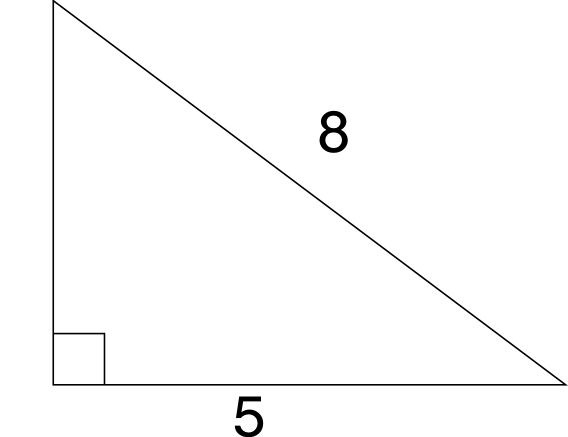
\includegraphics[width=10em]{ink/trigSubs/triangleValuesBottomHyp}
    \vfill
  \item 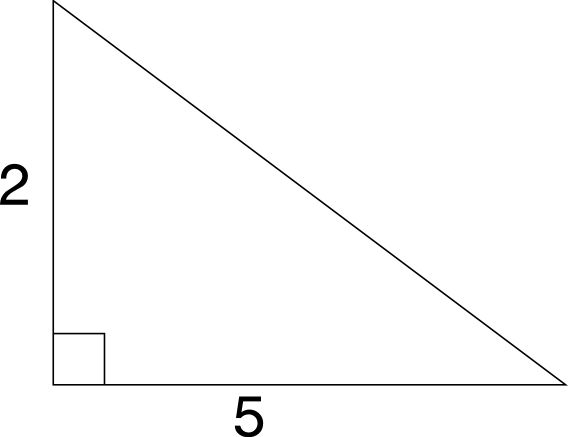
\includegraphics[width=10em]{ink/trigSubs/triangleValuesLeftBottom}
    \vfill
  \item 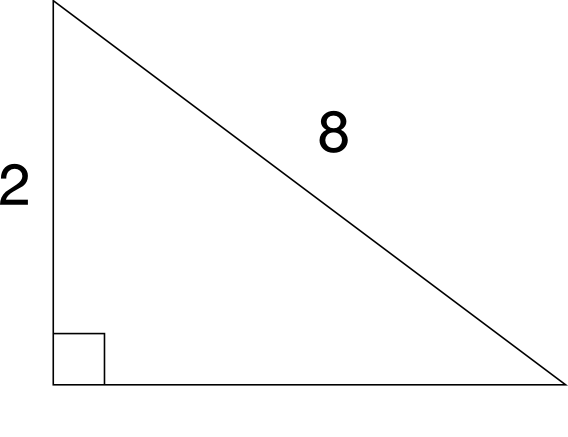
\includegraphics[width=10em]{ink/trigSubs/triangleValuesLeftHyp}
    \vfill
  \end{subproblem}
\end{problem}



\actTitle{Trigonometric Substitution}
\begin{problem}
  \item  A rod of length 2m has a uniform charge density, $\lambda_q$ C/m.
  The center of the rod is placed at the origin and is aligned along the
  $x$-axis.
  \begin{subproblem}
    \item Make a rough sketch of the rod.
         \vspace{5em}
   \item Divide the rod into $n$ equal parts, and determine the length of
         each part, and the coordinates for the endpoints.
         \vspace{2em}
     \item Mark a point 1m above the center of the rod in your picture. Determine the
         electric field due to the charge in one small piece of the rod.
         (Determine the $\vec{i}$ and $\vec{j}$ components separately.)
       \vfill
     \item Add up the components of the electic field to get a sum representing the
      $\vec{i}$ and $\vec{j}$ components of the electic field.
      \vfill
    \clearpage
    \item Determine the integrals that represent the $\vec{i}$ and $\vec{j}$ components of the electic field.
      Determine the values of the integrals and determine the electric field above the center of the rod.
      \vfill
  \end{subproblem}

\end{problem}

\postClass

\begin{problem}
\item Briefly state two ideas from today's class.
  \begin{itemize}
  \item
  \item
  \end{itemize}
  \item A rod has a charge distribution.
    The left endpoint is $x=0$m, and the right endpoint is
    $x=0.5$m. Determine the total charge in the rod for the following
    charge densities.
    \begin{subproblem}
      \item $\lambda_q = \frac{1}{\sqrt{1-x^2}}$ C/m
        \vfill
      \item $\lambda_q = \frac{1}{\sqrt{4-x^2}}$ C/m
        \vfill
    \end{subproblem}
  \item  A rod of length 4m has a uniform charge density, $\lambda_q$ C/m.
    The center of the rod is placed at the origin and is aligned along the
    $x$-axis.
    \begin{subproblem}
      \item Determine the electric field 1m above the center of the rod.
      \item Determine the electric field $l$m above the center of the rod,
        where $l$ is a constant.
      \item Determine the electric field at any point above the rod.
    \end{subproblem}

  \item  A rod of infinite length has a uniform charge density, $\lambda_q$ C/m.
      \begin{subproblem}
        \item Determine the electric field 1m above the rod.
        \item Determine the electric field $l$m above the rod,
          where $l$ is a constant.
        \item Determine the electric field at any point above the rod.
      \end{subproblem}


\end{problem}


%=========================================================================
% Trig substitutions - day 2
%=========================================================================
\preClass{Integraton}

\begin{problem}
\item For each of the triangles below, determine the length of the
  side with the missing length. Also, determine the sine, cosine, and tangent
    for the angle in the lower right part of the triangle.
  \begin{subproblem}
  \item 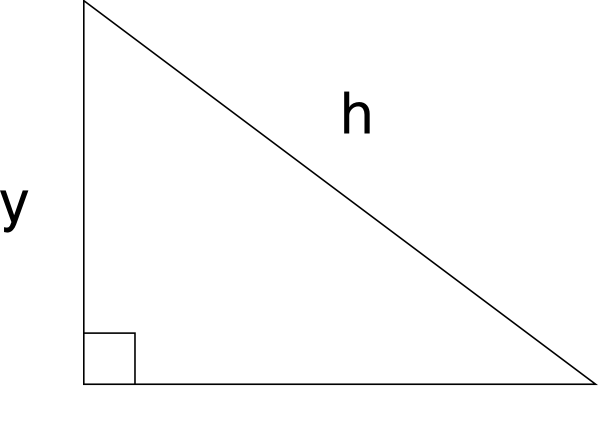
\includegraphics[width=10em]{ink/trigSubs/triangleSymbolsLeftHyp}
    \vfill
  \item 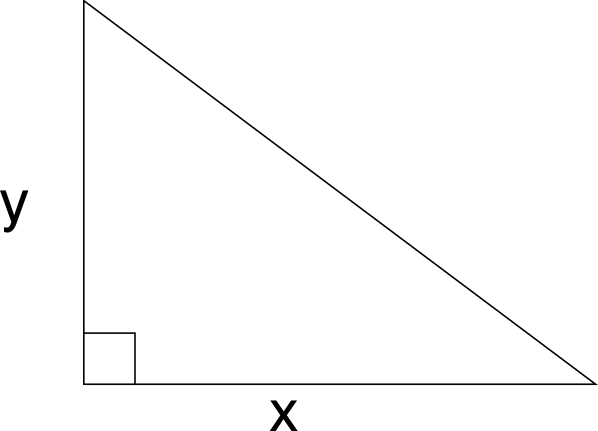
\includegraphics[width=10em]{ink/trigSubs/triangleSymbolsBottomLeft}
    \vfill
  \item 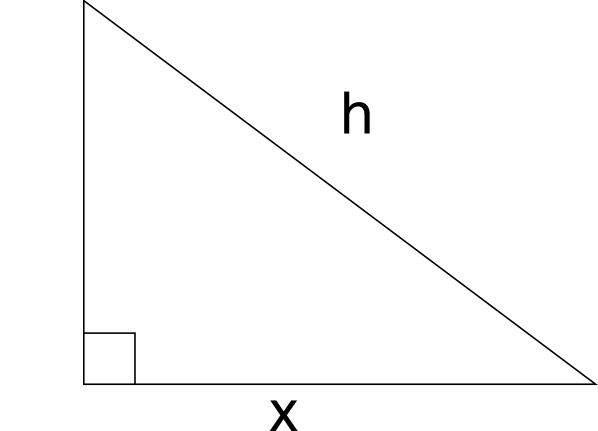
\includegraphics[width=10em]{ink/trigSubs/triangleSymbolsBottomHyp}
    \vfill
  \end{subproblem}
\end{problem}



\actTitle{Trigonometric Substitution}
\begin{problem}
  \item  A rod of length 4m has a uniform charge density, $\lambda_q$ C/m.
  The center of the rod is placed at the origin and is aligned along the
  $x$-axis.
  \begin{subproblem}
    \item Make a rough sketch of the rod.
         \vspace{5em}
   \item Divide the rod into $n$ equal parts, and determine the length of
         each part, and the coordinates for the endpoints.
         \vspace{2em}
     \item Mark a point 3m above the \textbf{right end} of the rod in your picture. Determine the
         electric field due to the charge in one small piece of the rod.
         (Determine the $\vec{i}$ and $\vec{j}$ components separately.)
       \vfill
     \item Add up the components of the electic field to get a sum representing the
      $\vec{i}$ and $\vec{j}$ components of the electic field.
      \vfill
    \clearpage
    \item Determine the integrals that represent the $\vec{i}$ and $\vec{j}$ components of the electic field at the point.
      Determine the values of the integrals and determine the electric field above the center of the rod.
      \vfill
  \end{subproblem}

\clearpage

\item A rod has a charge distribution, and the length of the rod is
  3m. The left endpoint is $x=0$m, and the right endpoint is
  $x=3$m. Determine the total charge in the rod for the following
  charge densities.
  \begin{subproblem}
    \item $\lambda_q = \frac{x}{\sqrt{9-x^2}}$ C/m
      \vfill
    \item $\lambda_q = \frac{x^2}{\sqrt{x^2-9}}$ C/m
      \vfill
  \end{subproblem}
\end{problem}

\postClass

\begin{problem}
\item Briefly state two ideas from today's class.
  \begin{itemize}
  \item
  \item
  \end{itemize}
\item A rod of length $l$ has a uniform charge density, $\lambda_q$ C/m,
    and the right side of the rod is located at the origin.
    \begin{subproblem}
      \item Determine the electric field $y$m above the right side of the rod,
        where $y$ is a constant.
      \item Determine what happens as the length $l$ gets extremely long.
        Does the electric field approach a particular value?
    \end{subproblem}
\item A rod has a charge distribution, and the length of the rod is
  2m. The left endpoint is $x=1$m, and the right endpoint is
  $x=1$m. Determine the total charge in the rod for the following
  charge densities.
  \begin{subproblem}
    \item $\lambda_q = \frac{x}{\sqrt{1+x^2}}$ C/m
      \vfill
    \item $\lambda_q = \frac{x^3}{\sqrt{4+x^2}}$ C/m
      \vfill
  \end{subproblem}
\end{problem}


%=========================================================================
% E-Field for a ring
%=========================================================================
\preClass{Arc-length of a circle.}

\begin{problem}
\item A person moves around a circle of radius 10m. Answer each of the questions below.
  \begin{subproblem}
  \item If the person moves around the whole circle how far has she traveled?
    \vfill
  \item If the person moves half way around the circle, through an angle of $\pi$, how far has she traveled?
    \vfill
  \item If the person moves around the circle through an angle of $\frac{\pi}{4}$ how far has she traveled?
    \vfill
  \item In general, if a person moves around a circle of radius $r$ through an angle $\theta$ how far has she traveled?
      \vfill
  \end{subproblem}
\end{problem}



\actTitle{Electric Field in Three Dimensions}
\begin{problem}
  \item  A thin, circular piece of metal has a uniform charge. The center of the circle is the origin,
        and it lies in the $x-y$ plane. The goal is to determine the electric field at a point above the
        center of the circle. The ring has a uniform charge, $\lambda_q$ C/m. \\
        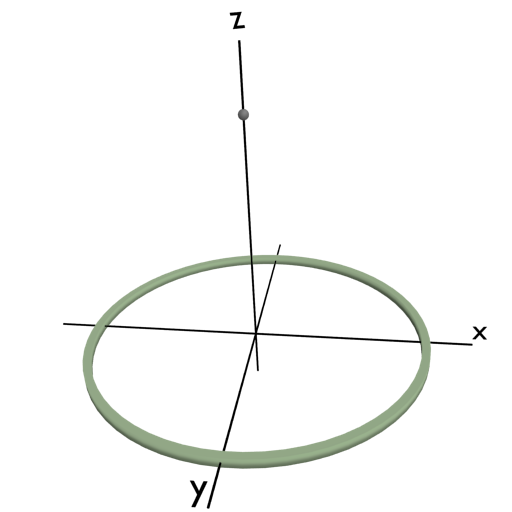
\includegraphics[width=15em]{blender/ringCharge}
  \begin{subproblem}
    \item Which direction do you think the electric field will point at the point above the circle? Why?
             \vspace{3em}
   \item The idea is to divide the ring into small pieces. Determine the charge in a small piece of the ring
       assuming that the length of the small piece is $\triangle s$. \\
           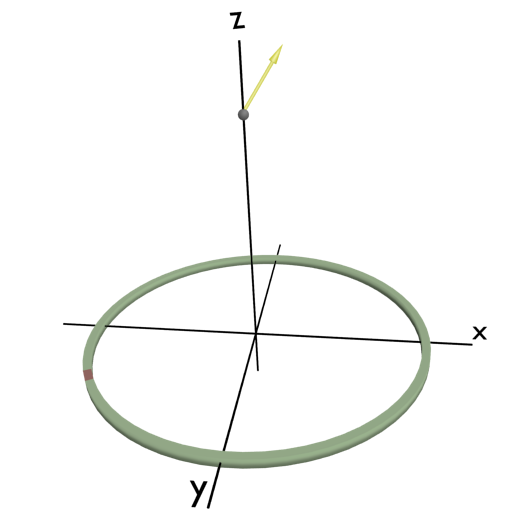
\includegraphics[width=10em]{blender/ringCharge-deltaE}

    \item If the point above the ring is a distance $l$ m over the origin and the radius of the circle is $r$,
      determine the magnitude of the electric field for the small piece. \\
        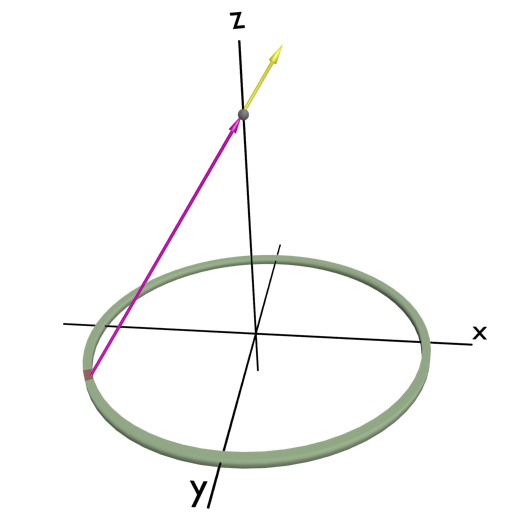
\includegraphics[width=10em]{blender/ringCharge-distance}

    \clearpage

     \item The electric field has three dimensions, components in the $\vec{i}$, $\vec{j}$, and $\vec{k}$ directions.
        The point above the ring is $l$ m above the center of the ring.
       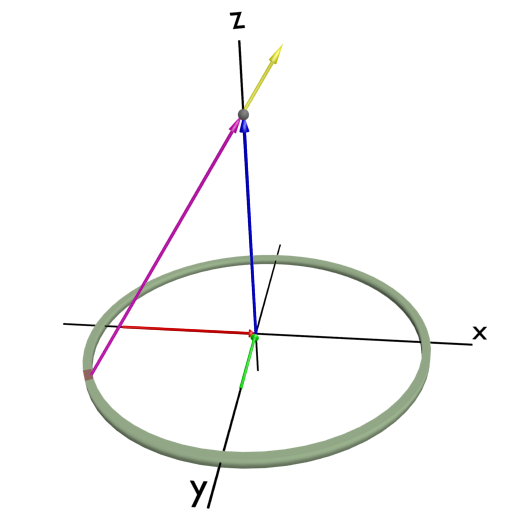
\includegraphics[width=15em]{blender/ringCharge-components}
       \begin{enumerate}
         \item Determine the component of $\triangle \vec{E}$ in the $z$-direction.
         \vfill
         \item Determine the component of $\triangle \vec{E}$ pointing in the direction from the small piece towards the origin in the $x-y$ plane.
         \vfill
         \item Determine the component of $\triangle \vec{E}$ in the $x$-direction.
         \vfill
         \item Determine the component of $\triangle \vec{E}$ in the $y$-direction.
         \vfill
       \end{enumerate}
       \clearpage
     \item Add up the components of the electic field to get a sum representing the
      $\vec{i}$ and $\vec{j}$ components of the electic field.
      \vfill
    \item Determine the length of the small piece of charge in terms of $r$ and $\triangle\theta$.
      \vspace{2em}
    \item  Determine the Riemann sum that approximates the $\vec{i}$, $\vec{j}$, and $\vec{k}$ components of the electic field at the point.
      \vspace{4em}
    \item Determine the integrals that represent the $\vec{i}$, $\vec{j}$, and $\vec{k}$ components of the electic field at the point.
      Determine the values of the integrals and determine the electric field above the center of the rod.
      \vfill
  \end{subproblem}

\clearpage

\item A rod has a charge distribution, and the length of the rod is
  3m. The left endpoint is $x=0$m, and the right endpoint is
  $x=3$m. Determine the total charge in the rod for the following
  charge densities.
  \begin{subproblem}
    \item $\lambda_q = \frac{x}{\sqrt{9-x^2}}$ C/m
      \vfill
    \item $\lambda_q = \frac{x^2}{\sqrt{x^2-9}}$ C/m
      \vfill
  \end{subproblem}
\end{problem}

\postClass

\begin{problem}
\item Briefly state two ideas from today's class.
  \begin{itemize}
  \item
  \item
  \end{itemize}
\item A rod of length $l$ has a uniform charge density, $\lambda_q$ C/m,
    and the right side of the rod is located at the origin.
    \begin{subproblem}
      \item Determine the electric field $y$m above the right side of the rod,
        where $y$ is a constant.
      \item Determine what happens as the length $l$ gets extremely long.
        Does the electric field approach a particular value?
    \end{subproblem}
\item A rod has a charge distribution, and the length of the rod is
  2m. The left endpoint is $x=1$m, and the right endpoint is
  $x=1$m. Determine the total charge in the rod for the following
  charge densities.
  \begin{subproblem}
    \item $\lambda_q = \frac{x}{\sqrt{1+x^2}}$ C/m
      \vfill
    \item $\lambda_q = \frac{x^3}{\sqrt{4+x^2}}$ C/m
      \vfill
  \end{subproblem}
\end{problem}


%=========================================================================
% Start of Volumes of Revolution
%=========================================================================
\preClass{Volumes of Revolution}

\begin{problem}
\item Determine the value of the integral
  \begin{eqnarray*}
    \int^h_0 \pi \left (R-\frac{R}{h} x\right)^2 ~ dx,
  \end{eqnarray*}
  where $h$ and $R$ are constants.
  \vfill

\item What is the volume of a right circular cylinder resting on its
  edge that has a radius of $R$ and a height $h$?

  \vfill

\item What is the volume of two cylinders resting on their edge
  standing next to each other? The first is a right circular cylinder
  that has a radius of $R_1$ and a height $h_1$, and the second is a
  right circular cylinder that has a radius of $R_2$ and a height
  $h_2$.

  \vfill

\end{problem}


\actTitle{Volumes of Revolution}
\begin{problem}
\item Determine the formula for a line that will be revolved
      around the $x$-axis, and the resulting solid will be a right
      circular cone of radius $R$ and height $h$.
  \begin{subproblem}
    \item Make a sketch of the line. (Make an axis and clear mark the
      axes.)
      \vfill

    \item Make a sketch of the resulting solid obtained after
      revolving the line around the $x$ axis.
      \vfill

    \item Determine the integral that represents the volume of the
      cone using washers.
      \vfill

  \end{subproblem}
\end{problem}

\postClass

\begin{problem}
\item Briefly state two ideas from today's class.
  \begin{itemize}
  \item
  \item
  \end{itemize}
\item
  \begin{subproblem}
    \item
  \end{subproblem}
\end{problem}


%=========================================================================
% Start of Volumes of Revolution
%=========================================================================
\preClass{Volumes of Revolution}

\begin{problem}
\item Determine the value of the integral
  \begin{eqnarray*}
    \int^R_0 2\pi x \left( R-x \right) ~ dx.
  \end{eqnarray*}
  \vfill

\item What is the volume of a right circular cylinder that has a
  radius of $R$ and a height $h$ that is resting on its base?

  \vfill

\item What is the volume of two cylinders stacked on top of one
  another vertically? The first is a right circular cylinder that has a radius of
  $R_1$ and a height $h_1$, and the second is a right circular cylinder that
  has a radius of $R_2$ and a height $h_2$.

  \vfill

\end{problem}


\actTitle{Volumes of Revolution}
\begin{problem}
\item Determine the formula for a line that will be revolved
      around the $y$-axis, and the resulting solid will be a right
      circular cone of radius $R$ and height $h$.
  \begin{subproblem}
    \item Make a sketch of the line. (Make an axis and clear mark the
      axes.)
      \vfill

    \item Make a sketch of the resulting solid obtained after
      revolving the line around the $y$ axis.
      \vfill

    \item Determine the integral that represents the volume of the
      cone using shells.
      \vfill

  \end{subproblem}
\end{problem}

\postClass

\begin{problem}
\item Briefly state two ideas from today's class.
  \begin{itemize}
  \item
  \item
  \end{itemize}
\item
  \begin{subproblem}
    \item
  \end{subproblem}
\end{problem}



%=========================================================================
% Start of Areas of Revolution
%=========================================================================
\preClass{Area of Revolution}

\begin{problem}
\item Determine the area of the sector of a circle shown below in
  terms of
  $\theta$ and $R$. \\
  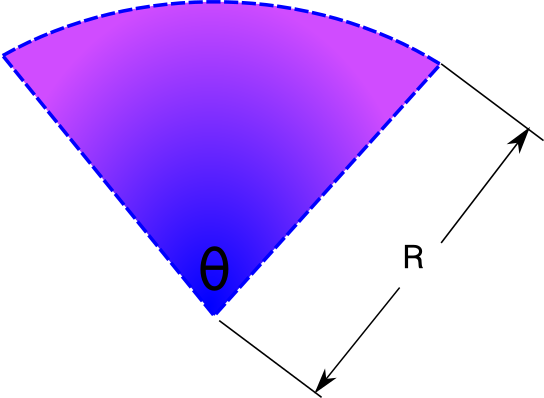
\includegraphics[width=12em]{ink/revolution/sector}

\item Determine the area of the slice of a sector shown below in terms of
  $\theta$, $L_1$, and $L_2$. \\
  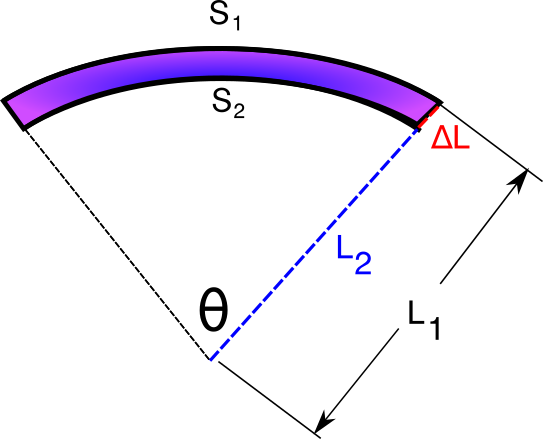
\includegraphics[width=12em]{ink/revolution/sectorDifference}

\item Use the relationship $L_2+\triangle L=L_1$ to express the area
  of the strip in terms of $\theta$, $\triangle L$, and  $L_2$.
  Expand and simplify the result.
  \label{problem:revol:area}
  \vfill

\item Substitute  $L_2\theta=S_2$  into the expression
  for the area in part \ref{problem:revol:area}.

  \vfill

\item Show that ${S_1-S_2}= \triangle L \theta$.

  \vfill


\item Substitute the expression found for $\triangle L \theta$ in the
  expression for the area. Simplify your result, and you should have a
  formula for the area of the strip only in terms of $S_1$, $S_2$, and
  $\triangle L$.

  \vfill

  \sideNote{Hint: $\triangle L^2\theta = \triangle L \cdot \triangle L \theta$}


\end{problem}


\actTitle{Area of Revolution}
\begin{problem}
\item Determine the formula for a line that will be revolved
      around the $x$-axis, and the resulting solid will be a right
      circular cone of radius $R$ and height $h$.
  \begin{subproblem}
    \item Make a sketch of the line. (Make an axis and clear mark the
      axes.)
      \vfill

    \item Make a sketch of the resulting solid obtained after
      revolving the line around the $y$ axis.
      \vfill

    \item Determine the integral that represents the area of the cone.
      \vfill

  \end{subproblem}
\end{problem}

\postClass

\begin{problem}
\item Briefly state two ideas from today's class.
  \begin{itemize}
  \item
  \item
  \end{itemize}
\item
  \begin{subproblem}
    \item
  \end{subproblem}
\end{problem}


%=========================================================================
% Start of partial fractions
%=========================================================================
\preClass{Rational Functions}

\begin{problem}
\item Express each function below as a single fraction. That is bring
  the two parts together over a common denominator and simplify the
  result.
  \begin{subproblem}
  \item $\frac{1}{x+3} + \frac{1}{x+2}$
    \vfill
  \item $\frac{1}{x+3} + \frac{3}{x-2}$
    \vfill
  \item $\frac{1}{x+3} + \frac{4}{x-3}$
    \vfill
  \end{subproblem}
\end{problem}


\actTitle{Partial Fractions}
\begin{problem}
\item Determine the common denominator for each of the expressions below.
  \begin{subproblem}
    \item $\frac{1}{x} + \frac{1}{x-3}$ \\
      Common Denominator: \framebox(250,50){~}
      \vfill
    \item $\frac{8}{x+7} + \frac{20}{x+50}$ \\
      Common Denominator: \framebox(250,50){~}
      \vfill
    \item $\frac{8,250}{x+7} + \frac{x}{x+50}$ \\
      Common Denominator: \framebox(250,50){~}
      \vfill
  \end{subproblem}

  \clearpage

\item For each of the following functions write the general form of
  the partial fraction expansion. The first one is completed as an
  example.
  \begin{subproblem}
    \item $\frac{2x+1}{x^2+2x-8}$ \\
      General Form: \framebox(250,50){$\frac{A}{x+4} + \frac{B}{x-2}$}
      \vfill
    \item $\frac{8x+1}{x^2-x-12}$ \\
      General Form: \framebox(250,50){~}
      \vfill
    \item $\frac{5x-10}{x^2-16}$ \\
      General Form: \framebox(250,50){~}
      \vfill
    \item $\frac{4x+2}{x^2-5x}$ \\
      General Form: \framebox(250,50){~}
      \vfill
  \end{subproblem}

\end{problem}

\postClass

\begin{problem}
\item Briefly state two ideas from today's class.
  \begin{itemize}
  \item
  \item
  \end{itemize}
\item
  \begin{subproblem}
    \item
  \end{subproblem}
\end{problem}


\preClass{Rational Functions}

\begin{problem}
\item Express each function below as a single fraction. That is bring
  the two parts together over a common denominator and simplify the
  result.
  \begin{subproblem}
  \item $\frac{1}{x+2} + \frac{3}{(x+2)^2}$
    \vfill
  \item $\frac{1}{x+3} + \frac{2}{(x+3)^2}$
    \vfill
  \item $\frac{1}{x} + \frac{1}{x^2} + \frac{1}{x^2}$
    \vfill
  \end{subproblem}
\end{problem}

\actTitle{Partial Fractions}
\begin{problem}
\item Determine the common denominator for each of the expressions below.
  \begin{subproblem}
    \item $\frac{1}{x-3} + \frac{1}{x^2-6x+9}$ \\
      Common Denominator: \framebox(250,50){~}
      \vfill
    \item $\frac{8}{x+7} + \frac{20}{x^2+14x+49}$ \\
      Common Denominator: \framebox(250,50){~}
      \vfill
    \item $\frac{8,250}{x+7} + \frac{x}{x^2+14x+49}$ \\
      Common Denominator: \framebox(250,50){~}
      \vfill
  \end{subproblem}

  \clearpage

\item For each of the following functions write the general form of
  the partial fraction expansion. The first one is completed as an
  example.
  \begin{subproblem}
    \item $\frac{2x+1}{x^2+2x-8}$ \\
      General Form: \framebox(250,50){$\frac{A}{x+4} + \frac{B}{x-2}$}
      \vfill
    \item $\frac{8x+1}{x^2-x-12}$ \\
      General Form: \framebox(250,50){~}
      \vfill
    \item $\frac{5x-10}{x^2+8x+16}$ \\
      General Form: \framebox(250,50){~}
      \vfill
    \item $\frac{4x+2}{x^2-10x+25}$ \\
      General Form: \framebox(250,50){~}
      \vfill
  \end{subproblem}

\end{problem}


\postClass

\begin{problem}
\item Briefly state two ideas from today's class.
  \begin{itemize}
  \item
  \item
  \end{itemize}
\item
  \begin{subproblem}
    \item
  \end{subproblem}
\end{problem}


\preClass{Rational Functions}

\begin{problem}
\item For each of the quadratic functions below complete the square to
  express each function in the form
  \begin{eqnarray*}
    f(x) & = & A(x-B)^2 + C.
  \end{eqnarray*}
  \begin{subproblem}
  \item $x^2 - 2x + 2$
    \vfill
  \item $x^2 - 6x + 12$
    \vfill
  \item $2x^2 - 4x + 6$
    \vfill
  \end{subproblem}
\end{problem}

\actTitle{Partial Fractions}
\begin{problem}
\item For each integral below complete the square on the denominator
  and then use $u$-substitution to determine the integral.
  \begin{subproblem}
    \item ${\displaystyle \int}\frac{1}{x^2 - 2x + 2}~dx$ \\
      \vfill
    \item ${\displaystyle\int}\frac{2}{x^2 - 6x + 12}~dx$ \\
      \vfill
    \item ${\displaystyle\int}\frac{1}{x^2 + 8x + 26}~dx$ \\
      \vfill
  \end{subproblem}

  \clearpage

\item Determine the value of the integral
  \begin{eqnarray*}
    \int \frac{1}{x^3+x^2+3\,x-5} ~ dx
  \end{eqnarray*}

  \vfill

\end{problem}


\postClass

\begin{problem}
\item Briefly state two ideas from today's class.
  \begin{itemize}
  \item
  \item
  \end{itemize}
\item
  \begin{subproblem}
    \item
  \end{subproblem}
\end{problem}





%%% Local Variables:
%%% mode: latex
%%% TeX-master: t
%%% End:



\chapter{Sequences and Series}
%=========================================================================
% Start of first day on sequences
%=========================================================================
\preClass{Sequences}

\begin{problem}
  \item Write out the numbers given by $\frac{(-1)^n}{n}$ where $n=1$,
    2, 3, 4, and 5.
    \vfill
  \item Determine a formula, $f(n)$, that matches the following
    numbers.
    \begin{eqnarray*}
      f(1) & = & 1, \\
      f(2) & = & \frac{1}{4}, \\
      f(3) & = & \frac{1}{9}, \\
      f(4) & = & \frac{1}{16}.
    \end{eqnarray*}
    \vfill
\end{problem}


\actTitle{Sequences}

\begin{problem}
\item A sequence of numbers, $\left\{ a_n \right\}_{n=1}^\infty$, is
  given by
  \begin{eqnarray*}
    a_n & = & \frac{\sin(n)}{n}.
  \end{eqnarray*}
  Plot the numbers on the axes below.

  \scalebox{0.75}{%% Creator: Matplotlib, PGF backend
%%
%% To include the figure in your LaTeX document, write
%%   \input{<filename>.pgf}
%%
%% Make sure the required packages are loaded in your preamble
%%   \usepackage{pgf}
%%
%% Figures using additional raster images can only be included by \input if
%% they are in the same directory as the main LaTeX file. For loading figures
%% from other directories you can use the `import` package
%%   \usepackage{import}
%% and then include the figures with
%%   \import{<path to file>}{<filename>.pgf}
%%
%% Matplotlib used the following preamble
%%   \usepackage{fontspec}
%%   \setmainfont{Bitstream Vera Serif}
%%   \setsansfont{Bitstream Vera Sans}
%%   \setmonofont{Bitstream Vera Sans Mono}
%%
\begingroup%
\makeatletter%
\begin{pgfpicture}%
\pgfpathrectangle{\pgfpointorigin}{\pgfqpoint{8.000000in}{6.000000in}}%
\pgfusepath{use as bounding box, clip}%
\begin{pgfscope}%
\pgfsetbuttcap%
\pgfsetmiterjoin%
\definecolor{currentfill}{rgb}{1.000000,1.000000,1.000000}%
\pgfsetfillcolor{currentfill}%
\pgfsetlinewidth{0.000000pt}%
\definecolor{currentstroke}{rgb}{1.000000,1.000000,1.000000}%
\pgfsetstrokecolor{currentstroke}%
\pgfsetdash{}{0pt}%
\pgfpathmoveto{\pgfqpoint{0.000000in}{0.000000in}}%
\pgfpathlineto{\pgfqpoint{8.000000in}{0.000000in}}%
\pgfpathlineto{\pgfqpoint{8.000000in}{6.000000in}}%
\pgfpathlineto{\pgfqpoint{0.000000in}{6.000000in}}%
\pgfpathclose%
\pgfusepath{fill}%
\end{pgfscope}%
\begin{pgfscope}%
\pgfsetbuttcap%
\pgfsetmiterjoin%
\definecolor{currentfill}{rgb}{1.000000,1.000000,1.000000}%
\pgfsetfillcolor{currentfill}%
\pgfsetlinewidth{0.000000pt}%
\definecolor{currentstroke}{rgb}{0.000000,0.000000,0.000000}%
\pgfsetstrokecolor{currentstroke}%
\pgfsetstrokeopacity{0.000000}%
\pgfsetdash{}{0pt}%
\pgfpathmoveto{\pgfqpoint{1.000000in}{0.600000in}}%
\pgfpathlineto{\pgfqpoint{7.200000in}{0.600000in}}%
\pgfpathlineto{\pgfqpoint{7.200000in}{5.400000in}}%
\pgfpathlineto{\pgfqpoint{1.000000in}{5.400000in}}%
\pgfpathclose%
\pgfusepath{fill}%
\end{pgfscope}%
\begin{pgfscope}%
\pgfsetrectcap%
\pgfsetmiterjoin%
\pgfsetlinewidth{1.003750pt}%
\definecolor{currentstroke}{rgb}{0.000000,0.000000,0.000000}%
\pgfsetstrokecolor{currentstroke}%
\pgfsetdash{}{0pt}%
\pgfpathmoveto{\pgfqpoint{1.000000in}{5.400000in}}%
\pgfpathlineto{\pgfqpoint{7.200000in}{5.400000in}}%
\pgfusepath{stroke}%
\end{pgfscope}%
\begin{pgfscope}%
\pgfsetrectcap%
\pgfsetmiterjoin%
\pgfsetlinewidth{1.003750pt}%
\definecolor{currentstroke}{rgb}{0.000000,0.000000,0.000000}%
\pgfsetstrokecolor{currentstroke}%
\pgfsetdash{}{0pt}%
\pgfpathmoveto{\pgfqpoint{7.200000in}{0.600000in}}%
\pgfpathlineto{\pgfqpoint{7.200000in}{5.400000in}}%
\pgfusepath{stroke}%
\end{pgfscope}%
\begin{pgfscope}%
\pgfsetrectcap%
\pgfsetmiterjoin%
\pgfsetlinewidth{1.003750pt}%
\definecolor{currentstroke}{rgb}{0.000000,0.000000,0.000000}%
\pgfsetstrokecolor{currentstroke}%
\pgfsetdash{}{0pt}%
\pgfpathmoveto{\pgfqpoint{1.000000in}{0.600000in}}%
\pgfpathlineto{\pgfqpoint{7.200000in}{0.600000in}}%
\pgfusepath{stroke}%
\end{pgfscope}%
\begin{pgfscope}%
\pgfsetrectcap%
\pgfsetmiterjoin%
\pgfsetlinewidth{1.003750pt}%
\definecolor{currentstroke}{rgb}{0.000000,0.000000,0.000000}%
\pgfsetstrokecolor{currentstroke}%
\pgfsetdash{}{0pt}%
\pgfpathmoveto{\pgfqpoint{1.000000in}{0.600000in}}%
\pgfpathlineto{\pgfqpoint{1.000000in}{5.400000in}}%
\pgfusepath{stroke}%
\end{pgfscope}%
\begin{pgfscope}%
\pgfpathrectangle{\pgfqpoint{1.000000in}{0.600000in}}{\pgfqpoint{6.200000in}{4.800000in}} %
\pgfusepath{clip}%
\pgfsetbuttcap%
\pgfsetroundjoin%
\pgfsetlinewidth{0.301125pt}%
\definecolor{currentstroke}{rgb}{0.000000,0.000000,0.000000}%
\pgfsetstrokecolor{currentstroke}%
\pgfsetdash{{6.000000pt}{6.000000pt}}{0.000000pt}%
\pgfpathmoveto{\pgfqpoint{1.086111in}{0.600000in}}%
\pgfpathlineto{\pgfqpoint{1.086111in}{5.400000in}}%
\pgfusepath{stroke}%
\end{pgfscope}%
\begin{pgfscope}%
\pgfsetbuttcap%
\pgfsetroundjoin%
\definecolor{currentfill}{rgb}{0.000000,0.000000,0.000000}%
\pgfsetfillcolor{currentfill}%
\pgfsetlinewidth{0.501875pt}%
\definecolor{currentstroke}{rgb}{0.000000,0.000000,0.000000}%
\pgfsetstrokecolor{currentstroke}%
\pgfsetdash{}{0pt}%
\pgfsys@defobject{currentmarker}{\pgfqpoint{0.000000in}{0.000000in}}{\pgfqpoint{0.000000in}{0.055556in}}{%
\pgfpathmoveto{\pgfqpoint{0.000000in}{0.000000in}}%
\pgfpathlineto{\pgfqpoint{0.000000in}{0.055556in}}%
\pgfusepath{stroke,fill}%
}%
\begin{pgfscope}%
\pgfsys@transformshift{1.086111in}{0.600000in}%
\pgfsys@useobject{currentmarker}{}%
\end{pgfscope}%
\end{pgfscope}%
\begin{pgfscope}%
\pgfsetbuttcap%
\pgfsetroundjoin%
\definecolor{currentfill}{rgb}{0.000000,0.000000,0.000000}%
\pgfsetfillcolor{currentfill}%
\pgfsetlinewidth{0.501875pt}%
\definecolor{currentstroke}{rgb}{0.000000,0.000000,0.000000}%
\pgfsetstrokecolor{currentstroke}%
\pgfsetdash{}{0pt}%
\pgfsys@defobject{currentmarker}{\pgfqpoint{0.000000in}{-0.055556in}}{\pgfqpoint{0.000000in}{0.000000in}}{%
\pgfpathmoveto{\pgfqpoint{0.000000in}{0.000000in}}%
\pgfpathlineto{\pgfqpoint{0.000000in}{-0.055556in}}%
\pgfusepath{stroke,fill}%
}%
\begin{pgfscope}%
\pgfsys@transformshift{1.086111in}{5.400000in}%
\pgfsys@useobject{currentmarker}{}%
\end{pgfscope}%
\end{pgfscope}%
\begin{pgfscope}%
\pgftext[x=1.086111in,y=0.544444in,,top]{\sffamily\fontsize{12.000000}{14.400000}\selectfont \(\displaystyle 0\)}%
\end{pgfscope}%
\begin{pgfscope}%
\pgfpathrectangle{\pgfqpoint{1.000000in}{0.600000in}}{\pgfqpoint{6.200000in}{4.800000in}} %
\pgfusepath{clip}%
\pgfsetbuttcap%
\pgfsetroundjoin%
\pgfsetlinewidth{0.301125pt}%
\definecolor{currentstroke}{rgb}{0.000000,0.000000,0.000000}%
\pgfsetstrokecolor{currentstroke}%
\pgfsetdash{{6.000000pt}{6.000000pt}}{0.000000pt}%
\pgfpathmoveto{\pgfqpoint{1.947222in}{0.600000in}}%
\pgfpathlineto{\pgfqpoint{1.947222in}{5.400000in}}%
\pgfusepath{stroke}%
\end{pgfscope}%
\begin{pgfscope}%
\pgfsetbuttcap%
\pgfsetroundjoin%
\definecolor{currentfill}{rgb}{0.000000,0.000000,0.000000}%
\pgfsetfillcolor{currentfill}%
\pgfsetlinewidth{0.501875pt}%
\definecolor{currentstroke}{rgb}{0.000000,0.000000,0.000000}%
\pgfsetstrokecolor{currentstroke}%
\pgfsetdash{}{0pt}%
\pgfsys@defobject{currentmarker}{\pgfqpoint{0.000000in}{0.000000in}}{\pgfqpoint{0.000000in}{0.055556in}}{%
\pgfpathmoveto{\pgfqpoint{0.000000in}{0.000000in}}%
\pgfpathlineto{\pgfqpoint{0.000000in}{0.055556in}}%
\pgfusepath{stroke,fill}%
}%
\begin{pgfscope}%
\pgfsys@transformshift{1.947222in}{0.600000in}%
\pgfsys@useobject{currentmarker}{}%
\end{pgfscope}%
\end{pgfscope}%
\begin{pgfscope}%
\pgfsetbuttcap%
\pgfsetroundjoin%
\definecolor{currentfill}{rgb}{0.000000,0.000000,0.000000}%
\pgfsetfillcolor{currentfill}%
\pgfsetlinewidth{0.501875pt}%
\definecolor{currentstroke}{rgb}{0.000000,0.000000,0.000000}%
\pgfsetstrokecolor{currentstroke}%
\pgfsetdash{}{0pt}%
\pgfsys@defobject{currentmarker}{\pgfqpoint{0.000000in}{-0.055556in}}{\pgfqpoint{0.000000in}{0.000000in}}{%
\pgfpathmoveto{\pgfqpoint{0.000000in}{0.000000in}}%
\pgfpathlineto{\pgfqpoint{0.000000in}{-0.055556in}}%
\pgfusepath{stroke,fill}%
}%
\begin{pgfscope}%
\pgfsys@transformshift{1.947222in}{5.400000in}%
\pgfsys@useobject{currentmarker}{}%
\end{pgfscope}%
\end{pgfscope}%
\begin{pgfscope}%
\pgftext[x=1.947222in,y=0.544444in,,top]{\sffamily\fontsize{12.000000}{14.400000}\selectfont \(\displaystyle 1\)}%
\end{pgfscope}%
\begin{pgfscope}%
\pgfpathrectangle{\pgfqpoint{1.000000in}{0.600000in}}{\pgfqpoint{6.200000in}{4.800000in}} %
\pgfusepath{clip}%
\pgfsetbuttcap%
\pgfsetroundjoin%
\pgfsetlinewidth{0.301125pt}%
\definecolor{currentstroke}{rgb}{0.000000,0.000000,0.000000}%
\pgfsetstrokecolor{currentstroke}%
\pgfsetdash{{6.000000pt}{6.000000pt}}{0.000000pt}%
\pgfpathmoveto{\pgfqpoint{2.808333in}{0.600000in}}%
\pgfpathlineto{\pgfqpoint{2.808333in}{5.400000in}}%
\pgfusepath{stroke}%
\end{pgfscope}%
\begin{pgfscope}%
\pgfsetbuttcap%
\pgfsetroundjoin%
\definecolor{currentfill}{rgb}{0.000000,0.000000,0.000000}%
\pgfsetfillcolor{currentfill}%
\pgfsetlinewidth{0.501875pt}%
\definecolor{currentstroke}{rgb}{0.000000,0.000000,0.000000}%
\pgfsetstrokecolor{currentstroke}%
\pgfsetdash{}{0pt}%
\pgfsys@defobject{currentmarker}{\pgfqpoint{0.000000in}{0.000000in}}{\pgfqpoint{0.000000in}{0.055556in}}{%
\pgfpathmoveto{\pgfqpoint{0.000000in}{0.000000in}}%
\pgfpathlineto{\pgfqpoint{0.000000in}{0.055556in}}%
\pgfusepath{stroke,fill}%
}%
\begin{pgfscope}%
\pgfsys@transformshift{2.808333in}{0.600000in}%
\pgfsys@useobject{currentmarker}{}%
\end{pgfscope}%
\end{pgfscope}%
\begin{pgfscope}%
\pgfsetbuttcap%
\pgfsetroundjoin%
\definecolor{currentfill}{rgb}{0.000000,0.000000,0.000000}%
\pgfsetfillcolor{currentfill}%
\pgfsetlinewidth{0.501875pt}%
\definecolor{currentstroke}{rgb}{0.000000,0.000000,0.000000}%
\pgfsetstrokecolor{currentstroke}%
\pgfsetdash{}{0pt}%
\pgfsys@defobject{currentmarker}{\pgfqpoint{0.000000in}{-0.055556in}}{\pgfqpoint{0.000000in}{0.000000in}}{%
\pgfpathmoveto{\pgfqpoint{0.000000in}{0.000000in}}%
\pgfpathlineto{\pgfqpoint{0.000000in}{-0.055556in}}%
\pgfusepath{stroke,fill}%
}%
\begin{pgfscope}%
\pgfsys@transformshift{2.808333in}{5.400000in}%
\pgfsys@useobject{currentmarker}{}%
\end{pgfscope}%
\end{pgfscope}%
\begin{pgfscope}%
\pgftext[x=2.808333in,y=0.544444in,,top]{\sffamily\fontsize{12.000000}{14.400000}\selectfont \(\displaystyle 2\)}%
\end{pgfscope}%
\begin{pgfscope}%
\pgfpathrectangle{\pgfqpoint{1.000000in}{0.600000in}}{\pgfqpoint{6.200000in}{4.800000in}} %
\pgfusepath{clip}%
\pgfsetbuttcap%
\pgfsetroundjoin%
\pgfsetlinewidth{0.301125pt}%
\definecolor{currentstroke}{rgb}{0.000000,0.000000,0.000000}%
\pgfsetstrokecolor{currentstroke}%
\pgfsetdash{{6.000000pt}{6.000000pt}}{0.000000pt}%
\pgfpathmoveto{\pgfqpoint{3.669444in}{0.600000in}}%
\pgfpathlineto{\pgfqpoint{3.669444in}{5.400000in}}%
\pgfusepath{stroke}%
\end{pgfscope}%
\begin{pgfscope}%
\pgfsetbuttcap%
\pgfsetroundjoin%
\definecolor{currentfill}{rgb}{0.000000,0.000000,0.000000}%
\pgfsetfillcolor{currentfill}%
\pgfsetlinewidth{0.501875pt}%
\definecolor{currentstroke}{rgb}{0.000000,0.000000,0.000000}%
\pgfsetstrokecolor{currentstroke}%
\pgfsetdash{}{0pt}%
\pgfsys@defobject{currentmarker}{\pgfqpoint{0.000000in}{0.000000in}}{\pgfqpoint{0.000000in}{0.055556in}}{%
\pgfpathmoveto{\pgfqpoint{0.000000in}{0.000000in}}%
\pgfpathlineto{\pgfqpoint{0.000000in}{0.055556in}}%
\pgfusepath{stroke,fill}%
}%
\begin{pgfscope}%
\pgfsys@transformshift{3.669444in}{0.600000in}%
\pgfsys@useobject{currentmarker}{}%
\end{pgfscope}%
\end{pgfscope}%
\begin{pgfscope}%
\pgfsetbuttcap%
\pgfsetroundjoin%
\definecolor{currentfill}{rgb}{0.000000,0.000000,0.000000}%
\pgfsetfillcolor{currentfill}%
\pgfsetlinewidth{0.501875pt}%
\definecolor{currentstroke}{rgb}{0.000000,0.000000,0.000000}%
\pgfsetstrokecolor{currentstroke}%
\pgfsetdash{}{0pt}%
\pgfsys@defobject{currentmarker}{\pgfqpoint{0.000000in}{-0.055556in}}{\pgfqpoint{0.000000in}{0.000000in}}{%
\pgfpathmoveto{\pgfqpoint{0.000000in}{0.000000in}}%
\pgfpathlineto{\pgfqpoint{0.000000in}{-0.055556in}}%
\pgfusepath{stroke,fill}%
}%
\begin{pgfscope}%
\pgfsys@transformshift{3.669444in}{5.400000in}%
\pgfsys@useobject{currentmarker}{}%
\end{pgfscope}%
\end{pgfscope}%
\begin{pgfscope}%
\pgftext[x=3.669444in,y=0.544444in,,top]{\sffamily\fontsize{12.000000}{14.400000}\selectfont \(\displaystyle 3\)}%
\end{pgfscope}%
\begin{pgfscope}%
\pgfpathrectangle{\pgfqpoint{1.000000in}{0.600000in}}{\pgfqpoint{6.200000in}{4.800000in}} %
\pgfusepath{clip}%
\pgfsetbuttcap%
\pgfsetroundjoin%
\pgfsetlinewidth{0.301125pt}%
\definecolor{currentstroke}{rgb}{0.000000,0.000000,0.000000}%
\pgfsetstrokecolor{currentstroke}%
\pgfsetdash{{6.000000pt}{6.000000pt}}{0.000000pt}%
\pgfpathmoveto{\pgfqpoint{4.530556in}{0.600000in}}%
\pgfpathlineto{\pgfqpoint{4.530556in}{5.400000in}}%
\pgfusepath{stroke}%
\end{pgfscope}%
\begin{pgfscope}%
\pgfsetbuttcap%
\pgfsetroundjoin%
\definecolor{currentfill}{rgb}{0.000000,0.000000,0.000000}%
\pgfsetfillcolor{currentfill}%
\pgfsetlinewidth{0.501875pt}%
\definecolor{currentstroke}{rgb}{0.000000,0.000000,0.000000}%
\pgfsetstrokecolor{currentstroke}%
\pgfsetdash{}{0pt}%
\pgfsys@defobject{currentmarker}{\pgfqpoint{0.000000in}{0.000000in}}{\pgfqpoint{0.000000in}{0.055556in}}{%
\pgfpathmoveto{\pgfqpoint{0.000000in}{0.000000in}}%
\pgfpathlineto{\pgfqpoint{0.000000in}{0.055556in}}%
\pgfusepath{stroke,fill}%
}%
\begin{pgfscope}%
\pgfsys@transformshift{4.530556in}{0.600000in}%
\pgfsys@useobject{currentmarker}{}%
\end{pgfscope}%
\end{pgfscope}%
\begin{pgfscope}%
\pgfsetbuttcap%
\pgfsetroundjoin%
\definecolor{currentfill}{rgb}{0.000000,0.000000,0.000000}%
\pgfsetfillcolor{currentfill}%
\pgfsetlinewidth{0.501875pt}%
\definecolor{currentstroke}{rgb}{0.000000,0.000000,0.000000}%
\pgfsetstrokecolor{currentstroke}%
\pgfsetdash{}{0pt}%
\pgfsys@defobject{currentmarker}{\pgfqpoint{0.000000in}{-0.055556in}}{\pgfqpoint{0.000000in}{0.000000in}}{%
\pgfpathmoveto{\pgfqpoint{0.000000in}{0.000000in}}%
\pgfpathlineto{\pgfqpoint{0.000000in}{-0.055556in}}%
\pgfusepath{stroke,fill}%
}%
\begin{pgfscope}%
\pgfsys@transformshift{4.530556in}{5.400000in}%
\pgfsys@useobject{currentmarker}{}%
\end{pgfscope}%
\end{pgfscope}%
\begin{pgfscope}%
\pgftext[x=4.530556in,y=0.544444in,,top]{\sffamily\fontsize{12.000000}{14.400000}\selectfont \(\displaystyle 4\)}%
\end{pgfscope}%
\begin{pgfscope}%
\pgfpathrectangle{\pgfqpoint{1.000000in}{0.600000in}}{\pgfqpoint{6.200000in}{4.800000in}} %
\pgfusepath{clip}%
\pgfsetbuttcap%
\pgfsetroundjoin%
\pgfsetlinewidth{0.301125pt}%
\definecolor{currentstroke}{rgb}{0.000000,0.000000,0.000000}%
\pgfsetstrokecolor{currentstroke}%
\pgfsetdash{{6.000000pt}{6.000000pt}}{0.000000pt}%
\pgfpathmoveto{\pgfqpoint{5.391667in}{0.600000in}}%
\pgfpathlineto{\pgfqpoint{5.391667in}{5.400000in}}%
\pgfusepath{stroke}%
\end{pgfscope}%
\begin{pgfscope}%
\pgfsetbuttcap%
\pgfsetroundjoin%
\definecolor{currentfill}{rgb}{0.000000,0.000000,0.000000}%
\pgfsetfillcolor{currentfill}%
\pgfsetlinewidth{0.501875pt}%
\definecolor{currentstroke}{rgb}{0.000000,0.000000,0.000000}%
\pgfsetstrokecolor{currentstroke}%
\pgfsetdash{}{0pt}%
\pgfsys@defobject{currentmarker}{\pgfqpoint{0.000000in}{0.000000in}}{\pgfqpoint{0.000000in}{0.055556in}}{%
\pgfpathmoveto{\pgfqpoint{0.000000in}{0.000000in}}%
\pgfpathlineto{\pgfqpoint{0.000000in}{0.055556in}}%
\pgfusepath{stroke,fill}%
}%
\begin{pgfscope}%
\pgfsys@transformshift{5.391667in}{0.600000in}%
\pgfsys@useobject{currentmarker}{}%
\end{pgfscope}%
\end{pgfscope}%
\begin{pgfscope}%
\pgfsetbuttcap%
\pgfsetroundjoin%
\definecolor{currentfill}{rgb}{0.000000,0.000000,0.000000}%
\pgfsetfillcolor{currentfill}%
\pgfsetlinewidth{0.501875pt}%
\definecolor{currentstroke}{rgb}{0.000000,0.000000,0.000000}%
\pgfsetstrokecolor{currentstroke}%
\pgfsetdash{}{0pt}%
\pgfsys@defobject{currentmarker}{\pgfqpoint{0.000000in}{-0.055556in}}{\pgfqpoint{0.000000in}{0.000000in}}{%
\pgfpathmoveto{\pgfqpoint{0.000000in}{0.000000in}}%
\pgfpathlineto{\pgfqpoint{0.000000in}{-0.055556in}}%
\pgfusepath{stroke,fill}%
}%
\begin{pgfscope}%
\pgfsys@transformshift{5.391667in}{5.400000in}%
\pgfsys@useobject{currentmarker}{}%
\end{pgfscope}%
\end{pgfscope}%
\begin{pgfscope}%
\pgftext[x=5.391667in,y=0.544444in,,top]{\sffamily\fontsize{12.000000}{14.400000}\selectfont \(\displaystyle 5\)}%
\end{pgfscope}%
\begin{pgfscope}%
\pgfpathrectangle{\pgfqpoint{1.000000in}{0.600000in}}{\pgfqpoint{6.200000in}{4.800000in}} %
\pgfusepath{clip}%
\pgfsetbuttcap%
\pgfsetroundjoin%
\pgfsetlinewidth{0.301125pt}%
\definecolor{currentstroke}{rgb}{0.000000,0.000000,0.000000}%
\pgfsetstrokecolor{currentstroke}%
\pgfsetdash{{6.000000pt}{6.000000pt}}{0.000000pt}%
\pgfpathmoveto{\pgfqpoint{6.252778in}{0.600000in}}%
\pgfpathlineto{\pgfqpoint{6.252778in}{5.400000in}}%
\pgfusepath{stroke}%
\end{pgfscope}%
\begin{pgfscope}%
\pgfsetbuttcap%
\pgfsetroundjoin%
\definecolor{currentfill}{rgb}{0.000000,0.000000,0.000000}%
\pgfsetfillcolor{currentfill}%
\pgfsetlinewidth{0.501875pt}%
\definecolor{currentstroke}{rgb}{0.000000,0.000000,0.000000}%
\pgfsetstrokecolor{currentstroke}%
\pgfsetdash{}{0pt}%
\pgfsys@defobject{currentmarker}{\pgfqpoint{0.000000in}{0.000000in}}{\pgfqpoint{0.000000in}{0.055556in}}{%
\pgfpathmoveto{\pgfqpoint{0.000000in}{0.000000in}}%
\pgfpathlineto{\pgfqpoint{0.000000in}{0.055556in}}%
\pgfusepath{stroke,fill}%
}%
\begin{pgfscope}%
\pgfsys@transformshift{6.252778in}{0.600000in}%
\pgfsys@useobject{currentmarker}{}%
\end{pgfscope}%
\end{pgfscope}%
\begin{pgfscope}%
\pgfsetbuttcap%
\pgfsetroundjoin%
\definecolor{currentfill}{rgb}{0.000000,0.000000,0.000000}%
\pgfsetfillcolor{currentfill}%
\pgfsetlinewidth{0.501875pt}%
\definecolor{currentstroke}{rgb}{0.000000,0.000000,0.000000}%
\pgfsetstrokecolor{currentstroke}%
\pgfsetdash{}{0pt}%
\pgfsys@defobject{currentmarker}{\pgfqpoint{0.000000in}{-0.055556in}}{\pgfqpoint{0.000000in}{0.000000in}}{%
\pgfpathmoveto{\pgfqpoint{0.000000in}{0.000000in}}%
\pgfpathlineto{\pgfqpoint{0.000000in}{-0.055556in}}%
\pgfusepath{stroke,fill}%
}%
\begin{pgfscope}%
\pgfsys@transformshift{6.252778in}{5.400000in}%
\pgfsys@useobject{currentmarker}{}%
\end{pgfscope}%
\end{pgfscope}%
\begin{pgfscope}%
\pgftext[x=6.252778in,y=0.544444in,,top]{\sffamily\fontsize{12.000000}{14.400000}\selectfont \(\displaystyle 6\)}%
\end{pgfscope}%
\begin{pgfscope}%
\pgfpathrectangle{\pgfqpoint{1.000000in}{0.600000in}}{\pgfqpoint{6.200000in}{4.800000in}} %
\pgfusepath{clip}%
\pgfsetbuttcap%
\pgfsetroundjoin%
\pgfsetlinewidth{0.301125pt}%
\definecolor{currentstroke}{rgb}{0.000000,0.000000,0.000000}%
\pgfsetstrokecolor{currentstroke}%
\pgfsetdash{{6.000000pt}{6.000000pt}}{0.000000pt}%
\pgfpathmoveto{\pgfqpoint{7.113889in}{0.600000in}}%
\pgfpathlineto{\pgfqpoint{7.113889in}{5.400000in}}%
\pgfusepath{stroke}%
\end{pgfscope}%
\begin{pgfscope}%
\pgfsetbuttcap%
\pgfsetroundjoin%
\definecolor{currentfill}{rgb}{0.000000,0.000000,0.000000}%
\pgfsetfillcolor{currentfill}%
\pgfsetlinewidth{0.501875pt}%
\definecolor{currentstroke}{rgb}{0.000000,0.000000,0.000000}%
\pgfsetstrokecolor{currentstroke}%
\pgfsetdash{}{0pt}%
\pgfsys@defobject{currentmarker}{\pgfqpoint{0.000000in}{0.000000in}}{\pgfqpoint{0.000000in}{0.055556in}}{%
\pgfpathmoveto{\pgfqpoint{0.000000in}{0.000000in}}%
\pgfpathlineto{\pgfqpoint{0.000000in}{0.055556in}}%
\pgfusepath{stroke,fill}%
}%
\begin{pgfscope}%
\pgfsys@transformshift{7.113889in}{0.600000in}%
\pgfsys@useobject{currentmarker}{}%
\end{pgfscope}%
\end{pgfscope}%
\begin{pgfscope}%
\pgfsetbuttcap%
\pgfsetroundjoin%
\definecolor{currentfill}{rgb}{0.000000,0.000000,0.000000}%
\pgfsetfillcolor{currentfill}%
\pgfsetlinewidth{0.501875pt}%
\definecolor{currentstroke}{rgb}{0.000000,0.000000,0.000000}%
\pgfsetstrokecolor{currentstroke}%
\pgfsetdash{}{0pt}%
\pgfsys@defobject{currentmarker}{\pgfqpoint{0.000000in}{-0.055556in}}{\pgfqpoint{0.000000in}{0.000000in}}{%
\pgfpathmoveto{\pgfqpoint{0.000000in}{0.000000in}}%
\pgfpathlineto{\pgfqpoint{0.000000in}{-0.055556in}}%
\pgfusepath{stroke,fill}%
}%
\begin{pgfscope}%
\pgfsys@transformshift{7.113889in}{5.400000in}%
\pgfsys@useobject{currentmarker}{}%
\end{pgfscope}%
\end{pgfscope}%
\begin{pgfscope}%
\pgftext[x=7.113889in,y=0.544444in,,top]{\sffamily\fontsize{12.000000}{14.400000}\selectfont \(\displaystyle 7\)}%
\end{pgfscope}%
\begin{pgfscope}%
\pgftext[x=4.100000in,y=0.313705in,,top]{\sffamily\fontsize{12.000000}{14.400000}\selectfont n}%
\end{pgfscope}%
\begin{pgfscope}%
\pgfpathrectangle{\pgfqpoint{1.000000in}{0.600000in}}{\pgfqpoint{6.200000in}{4.800000in}} %
\pgfusepath{clip}%
\pgfsetbuttcap%
\pgfsetroundjoin%
\pgfsetlinewidth{0.301125pt}%
\definecolor{currentstroke}{rgb}{0.000000,0.000000,0.000000}%
\pgfsetstrokecolor{currentstroke}%
\pgfsetdash{{6.000000pt}{6.000000pt}}{0.000000pt}%
\pgfpathmoveto{\pgfqpoint{1.000000in}{0.818182in}}%
\pgfpathlineto{\pgfqpoint{7.200000in}{0.818182in}}%
\pgfusepath{stroke}%
\end{pgfscope}%
\begin{pgfscope}%
\pgfsetbuttcap%
\pgfsetroundjoin%
\definecolor{currentfill}{rgb}{0.000000,0.000000,0.000000}%
\pgfsetfillcolor{currentfill}%
\pgfsetlinewidth{0.501875pt}%
\definecolor{currentstroke}{rgb}{0.000000,0.000000,0.000000}%
\pgfsetstrokecolor{currentstroke}%
\pgfsetdash{}{0pt}%
\pgfsys@defobject{currentmarker}{\pgfqpoint{0.000000in}{0.000000in}}{\pgfqpoint{0.055556in}{0.000000in}}{%
\pgfpathmoveto{\pgfqpoint{0.000000in}{0.000000in}}%
\pgfpathlineto{\pgfqpoint{0.055556in}{0.000000in}}%
\pgfusepath{stroke,fill}%
}%
\begin{pgfscope}%
\pgfsys@transformshift{1.000000in}{0.818182in}%
\pgfsys@useobject{currentmarker}{}%
\end{pgfscope}%
\end{pgfscope}%
\begin{pgfscope}%
\pgfsetbuttcap%
\pgfsetroundjoin%
\definecolor{currentfill}{rgb}{0.000000,0.000000,0.000000}%
\pgfsetfillcolor{currentfill}%
\pgfsetlinewidth{0.501875pt}%
\definecolor{currentstroke}{rgb}{0.000000,0.000000,0.000000}%
\pgfsetstrokecolor{currentstroke}%
\pgfsetdash{}{0pt}%
\pgfsys@defobject{currentmarker}{\pgfqpoint{-0.055556in}{0.000000in}}{\pgfqpoint{0.000000in}{0.000000in}}{%
\pgfpathmoveto{\pgfqpoint{0.000000in}{0.000000in}}%
\pgfpathlineto{\pgfqpoint{-0.055556in}{0.000000in}}%
\pgfusepath{stroke,fill}%
}%
\begin{pgfscope}%
\pgfsys@transformshift{7.200000in}{0.818182in}%
\pgfsys@useobject{currentmarker}{}%
\end{pgfscope}%
\end{pgfscope}%
\begin{pgfscope}%
\pgftext[x=0.944444in,y=0.818182in,right,]{\sffamily\fontsize{12.000000}{14.400000}\selectfont \(\displaystyle -1.0\)}%
\end{pgfscope}%
\begin{pgfscope}%
\pgfpathrectangle{\pgfqpoint{1.000000in}{0.600000in}}{\pgfqpoint{6.200000in}{4.800000in}} %
\pgfusepath{clip}%
\pgfsetbuttcap%
\pgfsetroundjoin%
\pgfsetlinewidth{0.301125pt}%
\definecolor{currentstroke}{rgb}{0.000000,0.000000,0.000000}%
\pgfsetstrokecolor{currentstroke}%
\pgfsetdash{{6.000000pt}{6.000000pt}}{0.000000pt}%
\pgfpathmoveto{\pgfqpoint{1.000000in}{1.254545in}}%
\pgfpathlineto{\pgfqpoint{7.200000in}{1.254545in}}%
\pgfusepath{stroke}%
\end{pgfscope}%
\begin{pgfscope}%
\pgfsetbuttcap%
\pgfsetroundjoin%
\definecolor{currentfill}{rgb}{0.000000,0.000000,0.000000}%
\pgfsetfillcolor{currentfill}%
\pgfsetlinewidth{0.501875pt}%
\definecolor{currentstroke}{rgb}{0.000000,0.000000,0.000000}%
\pgfsetstrokecolor{currentstroke}%
\pgfsetdash{}{0pt}%
\pgfsys@defobject{currentmarker}{\pgfqpoint{0.000000in}{0.000000in}}{\pgfqpoint{0.055556in}{0.000000in}}{%
\pgfpathmoveto{\pgfqpoint{0.000000in}{0.000000in}}%
\pgfpathlineto{\pgfqpoint{0.055556in}{0.000000in}}%
\pgfusepath{stroke,fill}%
}%
\begin{pgfscope}%
\pgfsys@transformshift{1.000000in}{1.254545in}%
\pgfsys@useobject{currentmarker}{}%
\end{pgfscope}%
\end{pgfscope}%
\begin{pgfscope}%
\pgfsetbuttcap%
\pgfsetroundjoin%
\definecolor{currentfill}{rgb}{0.000000,0.000000,0.000000}%
\pgfsetfillcolor{currentfill}%
\pgfsetlinewidth{0.501875pt}%
\definecolor{currentstroke}{rgb}{0.000000,0.000000,0.000000}%
\pgfsetstrokecolor{currentstroke}%
\pgfsetdash{}{0pt}%
\pgfsys@defobject{currentmarker}{\pgfqpoint{-0.055556in}{0.000000in}}{\pgfqpoint{0.000000in}{0.000000in}}{%
\pgfpathmoveto{\pgfqpoint{0.000000in}{0.000000in}}%
\pgfpathlineto{\pgfqpoint{-0.055556in}{0.000000in}}%
\pgfusepath{stroke,fill}%
}%
\begin{pgfscope}%
\pgfsys@transformshift{7.200000in}{1.254545in}%
\pgfsys@useobject{currentmarker}{}%
\end{pgfscope}%
\end{pgfscope}%
\begin{pgfscope}%
\pgftext[x=0.944444in,y=1.254545in,right,]{\sffamily\fontsize{12.000000}{14.400000}\selectfont \(\displaystyle -0.8\)}%
\end{pgfscope}%
\begin{pgfscope}%
\pgfpathrectangle{\pgfqpoint{1.000000in}{0.600000in}}{\pgfqpoint{6.200000in}{4.800000in}} %
\pgfusepath{clip}%
\pgfsetbuttcap%
\pgfsetroundjoin%
\pgfsetlinewidth{0.301125pt}%
\definecolor{currentstroke}{rgb}{0.000000,0.000000,0.000000}%
\pgfsetstrokecolor{currentstroke}%
\pgfsetdash{{6.000000pt}{6.000000pt}}{0.000000pt}%
\pgfpathmoveto{\pgfqpoint{1.000000in}{1.690909in}}%
\pgfpathlineto{\pgfqpoint{7.200000in}{1.690909in}}%
\pgfusepath{stroke}%
\end{pgfscope}%
\begin{pgfscope}%
\pgfsetbuttcap%
\pgfsetroundjoin%
\definecolor{currentfill}{rgb}{0.000000,0.000000,0.000000}%
\pgfsetfillcolor{currentfill}%
\pgfsetlinewidth{0.501875pt}%
\definecolor{currentstroke}{rgb}{0.000000,0.000000,0.000000}%
\pgfsetstrokecolor{currentstroke}%
\pgfsetdash{}{0pt}%
\pgfsys@defobject{currentmarker}{\pgfqpoint{0.000000in}{0.000000in}}{\pgfqpoint{0.055556in}{0.000000in}}{%
\pgfpathmoveto{\pgfqpoint{0.000000in}{0.000000in}}%
\pgfpathlineto{\pgfqpoint{0.055556in}{0.000000in}}%
\pgfusepath{stroke,fill}%
}%
\begin{pgfscope}%
\pgfsys@transformshift{1.000000in}{1.690909in}%
\pgfsys@useobject{currentmarker}{}%
\end{pgfscope}%
\end{pgfscope}%
\begin{pgfscope}%
\pgfsetbuttcap%
\pgfsetroundjoin%
\definecolor{currentfill}{rgb}{0.000000,0.000000,0.000000}%
\pgfsetfillcolor{currentfill}%
\pgfsetlinewidth{0.501875pt}%
\definecolor{currentstroke}{rgb}{0.000000,0.000000,0.000000}%
\pgfsetstrokecolor{currentstroke}%
\pgfsetdash{}{0pt}%
\pgfsys@defobject{currentmarker}{\pgfqpoint{-0.055556in}{0.000000in}}{\pgfqpoint{0.000000in}{0.000000in}}{%
\pgfpathmoveto{\pgfqpoint{0.000000in}{0.000000in}}%
\pgfpathlineto{\pgfqpoint{-0.055556in}{0.000000in}}%
\pgfusepath{stroke,fill}%
}%
\begin{pgfscope}%
\pgfsys@transformshift{7.200000in}{1.690909in}%
\pgfsys@useobject{currentmarker}{}%
\end{pgfscope}%
\end{pgfscope}%
\begin{pgfscope}%
\pgftext[x=0.944444in,y=1.690909in,right,]{\sffamily\fontsize{12.000000}{14.400000}\selectfont \(\displaystyle -0.6\)}%
\end{pgfscope}%
\begin{pgfscope}%
\pgfpathrectangle{\pgfqpoint{1.000000in}{0.600000in}}{\pgfqpoint{6.200000in}{4.800000in}} %
\pgfusepath{clip}%
\pgfsetbuttcap%
\pgfsetroundjoin%
\pgfsetlinewidth{0.301125pt}%
\definecolor{currentstroke}{rgb}{0.000000,0.000000,0.000000}%
\pgfsetstrokecolor{currentstroke}%
\pgfsetdash{{6.000000pt}{6.000000pt}}{0.000000pt}%
\pgfpathmoveto{\pgfqpoint{1.000000in}{2.127273in}}%
\pgfpathlineto{\pgfqpoint{7.200000in}{2.127273in}}%
\pgfusepath{stroke}%
\end{pgfscope}%
\begin{pgfscope}%
\pgfsetbuttcap%
\pgfsetroundjoin%
\definecolor{currentfill}{rgb}{0.000000,0.000000,0.000000}%
\pgfsetfillcolor{currentfill}%
\pgfsetlinewidth{0.501875pt}%
\definecolor{currentstroke}{rgb}{0.000000,0.000000,0.000000}%
\pgfsetstrokecolor{currentstroke}%
\pgfsetdash{}{0pt}%
\pgfsys@defobject{currentmarker}{\pgfqpoint{0.000000in}{0.000000in}}{\pgfqpoint{0.055556in}{0.000000in}}{%
\pgfpathmoveto{\pgfqpoint{0.000000in}{0.000000in}}%
\pgfpathlineto{\pgfqpoint{0.055556in}{0.000000in}}%
\pgfusepath{stroke,fill}%
}%
\begin{pgfscope}%
\pgfsys@transformshift{1.000000in}{2.127273in}%
\pgfsys@useobject{currentmarker}{}%
\end{pgfscope}%
\end{pgfscope}%
\begin{pgfscope}%
\pgfsetbuttcap%
\pgfsetroundjoin%
\definecolor{currentfill}{rgb}{0.000000,0.000000,0.000000}%
\pgfsetfillcolor{currentfill}%
\pgfsetlinewidth{0.501875pt}%
\definecolor{currentstroke}{rgb}{0.000000,0.000000,0.000000}%
\pgfsetstrokecolor{currentstroke}%
\pgfsetdash{}{0pt}%
\pgfsys@defobject{currentmarker}{\pgfqpoint{-0.055556in}{0.000000in}}{\pgfqpoint{0.000000in}{0.000000in}}{%
\pgfpathmoveto{\pgfqpoint{0.000000in}{0.000000in}}%
\pgfpathlineto{\pgfqpoint{-0.055556in}{0.000000in}}%
\pgfusepath{stroke,fill}%
}%
\begin{pgfscope}%
\pgfsys@transformshift{7.200000in}{2.127273in}%
\pgfsys@useobject{currentmarker}{}%
\end{pgfscope}%
\end{pgfscope}%
\begin{pgfscope}%
\pgftext[x=0.944444in,y=2.127273in,right,]{\sffamily\fontsize{12.000000}{14.400000}\selectfont \(\displaystyle -0.4\)}%
\end{pgfscope}%
\begin{pgfscope}%
\pgfpathrectangle{\pgfqpoint{1.000000in}{0.600000in}}{\pgfqpoint{6.200000in}{4.800000in}} %
\pgfusepath{clip}%
\pgfsetbuttcap%
\pgfsetroundjoin%
\pgfsetlinewidth{0.301125pt}%
\definecolor{currentstroke}{rgb}{0.000000,0.000000,0.000000}%
\pgfsetstrokecolor{currentstroke}%
\pgfsetdash{{6.000000pt}{6.000000pt}}{0.000000pt}%
\pgfpathmoveto{\pgfqpoint{1.000000in}{2.563636in}}%
\pgfpathlineto{\pgfqpoint{7.200000in}{2.563636in}}%
\pgfusepath{stroke}%
\end{pgfscope}%
\begin{pgfscope}%
\pgfsetbuttcap%
\pgfsetroundjoin%
\definecolor{currentfill}{rgb}{0.000000,0.000000,0.000000}%
\pgfsetfillcolor{currentfill}%
\pgfsetlinewidth{0.501875pt}%
\definecolor{currentstroke}{rgb}{0.000000,0.000000,0.000000}%
\pgfsetstrokecolor{currentstroke}%
\pgfsetdash{}{0pt}%
\pgfsys@defobject{currentmarker}{\pgfqpoint{0.000000in}{0.000000in}}{\pgfqpoint{0.055556in}{0.000000in}}{%
\pgfpathmoveto{\pgfqpoint{0.000000in}{0.000000in}}%
\pgfpathlineto{\pgfqpoint{0.055556in}{0.000000in}}%
\pgfusepath{stroke,fill}%
}%
\begin{pgfscope}%
\pgfsys@transformshift{1.000000in}{2.563636in}%
\pgfsys@useobject{currentmarker}{}%
\end{pgfscope}%
\end{pgfscope}%
\begin{pgfscope}%
\pgfsetbuttcap%
\pgfsetroundjoin%
\definecolor{currentfill}{rgb}{0.000000,0.000000,0.000000}%
\pgfsetfillcolor{currentfill}%
\pgfsetlinewidth{0.501875pt}%
\definecolor{currentstroke}{rgb}{0.000000,0.000000,0.000000}%
\pgfsetstrokecolor{currentstroke}%
\pgfsetdash{}{0pt}%
\pgfsys@defobject{currentmarker}{\pgfqpoint{-0.055556in}{0.000000in}}{\pgfqpoint{0.000000in}{0.000000in}}{%
\pgfpathmoveto{\pgfqpoint{0.000000in}{0.000000in}}%
\pgfpathlineto{\pgfqpoint{-0.055556in}{0.000000in}}%
\pgfusepath{stroke,fill}%
}%
\begin{pgfscope}%
\pgfsys@transformshift{7.200000in}{2.563636in}%
\pgfsys@useobject{currentmarker}{}%
\end{pgfscope}%
\end{pgfscope}%
\begin{pgfscope}%
\pgftext[x=0.944444in,y=2.563636in,right,]{\sffamily\fontsize{12.000000}{14.400000}\selectfont \(\displaystyle -0.2\)}%
\end{pgfscope}%
\begin{pgfscope}%
\pgfpathrectangle{\pgfqpoint{1.000000in}{0.600000in}}{\pgfqpoint{6.200000in}{4.800000in}} %
\pgfusepath{clip}%
\pgfsetbuttcap%
\pgfsetroundjoin%
\pgfsetlinewidth{0.301125pt}%
\definecolor{currentstroke}{rgb}{0.000000,0.000000,0.000000}%
\pgfsetstrokecolor{currentstroke}%
\pgfsetdash{{6.000000pt}{6.000000pt}}{0.000000pt}%
\pgfpathmoveto{\pgfqpoint{1.000000in}{3.000000in}}%
\pgfpathlineto{\pgfqpoint{7.200000in}{3.000000in}}%
\pgfusepath{stroke}%
\end{pgfscope}%
\begin{pgfscope}%
\pgfsetbuttcap%
\pgfsetroundjoin%
\definecolor{currentfill}{rgb}{0.000000,0.000000,0.000000}%
\pgfsetfillcolor{currentfill}%
\pgfsetlinewidth{0.501875pt}%
\definecolor{currentstroke}{rgb}{0.000000,0.000000,0.000000}%
\pgfsetstrokecolor{currentstroke}%
\pgfsetdash{}{0pt}%
\pgfsys@defobject{currentmarker}{\pgfqpoint{0.000000in}{0.000000in}}{\pgfqpoint{0.055556in}{0.000000in}}{%
\pgfpathmoveto{\pgfqpoint{0.000000in}{0.000000in}}%
\pgfpathlineto{\pgfqpoint{0.055556in}{0.000000in}}%
\pgfusepath{stroke,fill}%
}%
\begin{pgfscope}%
\pgfsys@transformshift{1.000000in}{3.000000in}%
\pgfsys@useobject{currentmarker}{}%
\end{pgfscope}%
\end{pgfscope}%
\begin{pgfscope}%
\pgfsetbuttcap%
\pgfsetroundjoin%
\definecolor{currentfill}{rgb}{0.000000,0.000000,0.000000}%
\pgfsetfillcolor{currentfill}%
\pgfsetlinewidth{0.501875pt}%
\definecolor{currentstroke}{rgb}{0.000000,0.000000,0.000000}%
\pgfsetstrokecolor{currentstroke}%
\pgfsetdash{}{0pt}%
\pgfsys@defobject{currentmarker}{\pgfqpoint{-0.055556in}{0.000000in}}{\pgfqpoint{0.000000in}{0.000000in}}{%
\pgfpathmoveto{\pgfqpoint{0.000000in}{0.000000in}}%
\pgfpathlineto{\pgfqpoint{-0.055556in}{0.000000in}}%
\pgfusepath{stroke,fill}%
}%
\begin{pgfscope}%
\pgfsys@transformshift{7.200000in}{3.000000in}%
\pgfsys@useobject{currentmarker}{}%
\end{pgfscope}%
\end{pgfscope}%
\begin{pgfscope}%
\pgftext[x=0.944444in,y=3.000000in,right,]{\sffamily\fontsize{12.000000}{14.400000}\selectfont \(\displaystyle 0.0\)}%
\end{pgfscope}%
\begin{pgfscope}%
\pgfpathrectangle{\pgfqpoint{1.000000in}{0.600000in}}{\pgfqpoint{6.200000in}{4.800000in}} %
\pgfusepath{clip}%
\pgfsetbuttcap%
\pgfsetroundjoin%
\pgfsetlinewidth{0.301125pt}%
\definecolor{currentstroke}{rgb}{0.000000,0.000000,0.000000}%
\pgfsetstrokecolor{currentstroke}%
\pgfsetdash{{6.000000pt}{6.000000pt}}{0.000000pt}%
\pgfpathmoveto{\pgfqpoint{1.000000in}{3.436364in}}%
\pgfpathlineto{\pgfqpoint{7.200000in}{3.436364in}}%
\pgfusepath{stroke}%
\end{pgfscope}%
\begin{pgfscope}%
\pgfsetbuttcap%
\pgfsetroundjoin%
\definecolor{currentfill}{rgb}{0.000000,0.000000,0.000000}%
\pgfsetfillcolor{currentfill}%
\pgfsetlinewidth{0.501875pt}%
\definecolor{currentstroke}{rgb}{0.000000,0.000000,0.000000}%
\pgfsetstrokecolor{currentstroke}%
\pgfsetdash{}{0pt}%
\pgfsys@defobject{currentmarker}{\pgfqpoint{0.000000in}{0.000000in}}{\pgfqpoint{0.055556in}{0.000000in}}{%
\pgfpathmoveto{\pgfqpoint{0.000000in}{0.000000in}}%
\pgfpathlineto{\pgfqpoint{0.055556in}{0.000000in}}%
\pgfusepath{stroke,fill}%
}%
\begin{pgfscope}%
\pgfsys@transformshift{1.000000in}{3.436364in}%
\pgfsys@useobject{currentmarker}{}%
\end{pgfscope}%
\end{pgfscope}%
\begin{pgfscope}%
\pgfsetbuttcap%
\pgfsetroundjoin%
\definecolor{currentfill}{rgb}{0.000000,0.000000,0.000000}%
\pgfsetfillcolor{currentfill}%
\pgfsetlinewidth{0.501875pt}%
\definecolor{currentstroke}{rgb}{0.000000,0.000000,0.000000}%
\pgfsetstrokecolor{currentstroke}%
\pgfsetdash{}{0pt}%
\pgfsys@defobject{currentmarker}{\pgfqpoint{-0.055556in}{0.000000in}}{\pgfqpoint{0.000000in}{0.000000in}}{%
\pgfpathmoveto{\pgfqpoint{0.000000in}{0.000000in}}%
\pgfpathlineto{\pgfqpoint{-0.055556in}{0.000000in}}%
\pgfusepath{stroke,fill}%
}%
\begin{pgfscope}%
\pgfsys@transformshift{7.200000in}{3.436364in}%
\pgfsys@useobject{currentmarker}{}%
\end{pgfscope}%
\end{pgfscope}%
\begin{pgfscope}%
\pgftext[x=0.944444in,y=3.436364in,right,]{\sffamily\fontsize{12.000000}{14.400000}\selectfont \(\displaystyle 0.2\)}%
\end{pgfscope}%
\begin{pgfscope}%
\pgfpathrectangle{\pgfqpoint{1.000000in}{0.600000in}}{\pgfqpoint{6.200000in}{4.800000in}} %
\pgfusepath{clip}%
\pgfsetbuttcap%
\pgfsetroundjoin%
\pgfsetlinewidth{0.301125pt}%
\definecolor{currentstroke}{rgb}{0.000000,0.000000,0.000000}%
\pgfsetstrokecolor{currentstroke}%
\pgfsetdash{{6.000000pt}{6.000000pt}}{0.000000pt}%
\pgfpathmoveto{\pgfqpoint{1.000000in}{3.872727in}}%
\pgfpathlineto{\pgfqpoint{7.200000in}{3.872727in}}%
\pgfusepath{stroke}%
\end{pgfscope}%
\begin{pgfscope}%
\pgfsetbuttcap%
\pgfsetroundjoin%
\definecolor{currentfill}{rgb}{0.000000,0.000000,0.000000}%
\pgfsetfillcolor{currentfill}%
\pgfsetlinewidth{0.501875pt}%
\definecolor{currentstroke}{rgb}{0.000000,0.000000,0.000000}%
\pgfsetstrokecolor{currentstroke}%
\pgfsetdash{}{0pt}%
\pgfsys@defobject{currentmarker}{\pgfqpoint{0.000000in}{0.000000in}}{\pgfqpoint{0.055556in}{0.000000in}}{%
\pgfpathmoveto{\pgfqpoint{0.000000in}{0.000000in}}%
\pgfpathlineto{\pgfqpoint{0.055556in}{0.000000in}}%
\pgfusepath{stroke,fill}%
}%
\begin{pgfscope}%
\pgfsys@transformshift{1.000000in}{3.872727in}%
\pgfsys@useobject{currentmarker}{}%
\end{pgfscope}%
\end{pgfscope}%
\begin{pgfscope}%
\pgfsetbuttcap%
\pgfsetroundjoin%
\definecolor{currentfill}{rgb}{0.000000,0.000000,0.000000}%
\pgfsetfillcolor{currentfill}%
\pgfsetlinewidth{0.501875pt}%
\definecolor{currentstroke}{rgb}{0.000000,0.000000,0.000000}%
\pgfsetstrokecolor{currentstroke}%
\pgfsetdash{}{0pt}%
\pgfsys@defobject{currentmarker}{\pgfqpoint{-0.055556in}{0.000000in}}{\pgfqpoint{0.000000in}{0.000000in}}{%
\pgfpathmoveto{\pgfqpoint{0.000000in}{0.000000in}}%
\pgfpathlineto{\pgfqpoint{-0.055556in}{0.000000in}}%
\pgfusepath{stroke,fill}%
}%
\begin{pgfscope}%
\pgfsys@transformshift{7.200000in}{3.872727in}%
\pgfsys@useobject{currentmarker}{}%
\end{pgfscope}%
\end{pgfscope}%
\begin{pgfscope}%
\pgftext[x=0.944444in,y=3.872727in,right,]{\sffamily\fontsize{12.000000}{14.400000}\selectfont \(\displaystyle 0.4\)}%
\end{pgfscope}%
\begin{pgfscope}%
\pgfpathrectangle{\pgfqpoint{1.000000in}{0.600000in}}{\pgfqpoint{6.200000in}{4.800000in}} %
\pgfusepath{clip}%
\pgfsetbuttcap%
\pgfsetroundjoin%
\pgfsetlinewidth{0.301125pt}%
\definecolor{currentstroke}{rgb}{0.000000,0.000000,0.000000}%
\pgfsetstrokecolor{currentstroke}%
\pgfsetdash{{6.000000pt}{6.000000pt}}{0.000000pt}%
\pgfpathmoveto{\pgfqpoint{1.000000in}{4.309091in}}%
\pgfpathlineto{\pgfqpoint{7.200000in}{4.309091in}}%
\pgfusepath{stroke}%
\end{pgfscope}%
\begin{pgfscope}%
\pgfsetbuttcap%
\pgfsetroundjoin%
\definecolor{currentfill}{rgb}{0.000000,0.000000,0.000000}%
\pgfsetfillcolor{currentfill}%
\pgfsetlinewidth{0.501875pt}%
\definecolor{currentstroke}{rgb}{0.000000,0.000000,0.000000}%
\pgfsetstrokecolor{currentstroke}%
\pgfsetdash{}{0pt}%
\pgfsys@defobject{currentmarker}{\pgfqpoint{0.000000in}{0.000000in}}{\pgfqpoint{0.055556in}{0.000000in}}{%
\pgfpathmoveto{\pgfqpoint{0.000000in}{0.000000in}}%
\pgfpathlineto{\pgfqpoint{0.055556in}{0.000000in}}%
\pgfusepath{stroke,fill}%
}%
\begin{pgfscope}%
\pgfsys@transformshift{1.000000in}{4.309091in}%
\pgfsys@useobject{currentmarker}{}%
\end{pgfscope}%
\end{pgfscope}%
\begin{pgfscope}%
\pgfsetbuttcap%
\pgfsetroundjoin%
\definecolor{currentfill}{rgb}{0.000000,0.000000,0.000000}%
\pgfsetfillcolor{currentfill}%
\pgfsetlinewidth{0.501875pt}%
\definecolor{currentstroke}{rgb}{0.000000,0.000000,0.000000}%
\pgfsetstrokecolor{currentstroke}%
\pgfsetdash{}{0pt}%
\pgfsys@defobject{currentmarker}{\pgfqpoint{-0.055556in}{0.000000in}}{\pgfqpoint{0.000000in}{0.000000in}}{%
\pgfpathmoveto{\pgfqpoint{0.000000in}{0.000000in}}%
\pgfpathlineto{\pgfqpoint{-0.055556in}{0.000000in}}%
\pgfusepath{stroke,fill}%
}%
\begin{pgfscope}%
\pgfsys@transformshift{7.200000in}{4.309091in}%
\pgfsys@useobject{currentmarker}{}%
\end{pgfscope}%
\end{pgfscope}%
\begin{pgfscope}%
\pgftext[x=0.944444in,y=4.309091in,right,]{\sffamily\fontsize{12.000000}{14.400000}\selectfont \(\displaystyle 0.6\)}%
\end{pgfscope}%
\begin{pgfscope}%
\pgfpathrectangle{\pgfqpoint{1.000000in}{0.600000in}}{\pgfqpoint{6.200000in}{4.800000in}} %
\pgfusepath{clip}%
\pgfsetbuttcap%
\pgfsetroundjoin%
\pgfsetlinewidth{0.301125pt}%
\definecolor{currentstroke}{rgb}{0.000000,0.000000,0.000000}%
\pgfsetstrokecolor{currentstroke}%
\pgfsetdash{{6.000000pt}{6.000000pt}}{0.000000pt}%
\pgfpathmoveto{\pgfqpoint{1.000000in}{4.745455in}}%
\pgfpathlineto{\pgfqpoint{7.200000in}{4.745455in}}%
\pgfusepath{stroke}%
\end{pgfscope}%
\begin{pgfscope}%
\pgfsetbuttcap%
\pgfsetroundjoin%
\definecolor{currentfill}{rgb}{0.000000,0.000000,0.000000}%
\pgfsetfillcolor{currentfill}%
\pgfsetlinewidth{0.501875pt}%
\definecolor{currentstroke}{rgb}{0.000000,0.000000,0.000000}%
\pgfsetstrokecolor{currentstroke}%
\pgfsetdash{}{0pt}%
\pgfsys@defobject{currentmarker}{\pgfqpoint{0.000000in}{0.000000in}}{\pgfqpoint{0.055556in}{0.000000in}}{%
\pgfpathmoveto{\pgfqpoint{0.000000in}{0.000000in}}%
\pgfpathlineto{\pgfqpoint{0.055556in}{0.000000in}}%
\pgfusepath{stroke,fill}%
}%
\begin{pgfscope}%
\pgfsys@transformshift{1.000000in}{4.745455in}%
\pgfsys@useobject{currentmarker}{}%
\end{pgfscope}%
\end{pgfscope}%
\begin{pgfscope}%
\pgfsetbuttcap%
\pgfsetroundjoin%
\definecolor{currentfill}{rgb}{0.000000,0.000000,0.000000}%
\pgfsetfillcolor{currentfill}%
\pgfsetlinewidth{0.501875pt}%
\definecolor{currentstroke}{rgb}{0.000000,0.000000,0.000000}%
\pgfsetstrokecolor{currentstroke}%
\pgfsetdash{}{0pt}%
\pgfsys@defobject{currentmarker}{\pgfqpoint{-0.055556in}{0.000000in}}{\pgfqpoint{0.000000in}{0.000000in}}{%
\pgfpathmoveto{\pgfqpoint{0.000000in}{0.000000in}}%
\pgfpathlineto{\pgfqpoint{-0.055556in}{0.000000in}}%
\pgfusepath{stroke,fill}%
}%
\begin{pgfscope}%
\pgfsys@transformshift{7.200000in}{4.745455in}%
\pgfsys@useobject{currentmarker}{}%
\end{pgfscope}%
\end{pgfscope}%
\begin{pgfscope}%
\pgftext[x=0.944444in,y=4.745455in,right,]{\sffamily\fontsize{12.000000}{14.400000}\selectfont \(\displaystyle 0.8\)}%
\end{pgfscope}%
\begin{pgfscope}%
\pgfpathrectangle{\pgfqpoint{1.000000in}{0.600000in}}{\pgfqpoint{6.200000in}{4.800000in}} %
\pgfusepath{clip}%
\pgfsetbuttcap%
\pgfsetroundjoin%
\pgfsetlinewidth{0.301125pt}%
\definecolor{currentstroke}{rgb}{0.000000,0.000000,0.000000}%
\pgfsetstrokecolor{currentstroke}%
\pgfsetdash{{6.000000pt}{6.000000pt}}{0.000000pt}%
\pgfpathmoveto{\pgfqpoint{1.000000in}{5.181818in}}%
\pgfpathlineto{\pgfqpoint{7.200000in}{5.181818in}}%
\pgfusepath{stroke}%
\end{pgfscope}%
\begin{pgfscope}%
\pgfsetbuttcap%
\pgfsetroundjoin%
\definecolor{currentfill}{rgb}{0.000000,0.000000,0.000000}%
\pgfsetfillcolor{currentfill}%
\pgfsetlinewidth{0.501875pt}%
\definecolor{currentstroke}{rgb}{0.000000,0.000000,0.000000}%
\pgfsetstrokecolor{currentstroke}%
\pgfsetdash{}{0pt}%
\pgfsys@defobject{currentmarker}{\pgfqpoint{0.000000in}{0.000000in}}{\pgfqpoint{0.055556in}{0.000000in}}{%
\pgfpathmoveto{\pgfqpoint{0.000000in}{0.000000in}}%
\pgfpathlineto{\pgfqpoint{0.055556in}{0.000000in}}%
\pgfusepath{stroke,fill}%
}%
\begin{pgfscope}%
\pgfsys@transformshift{1.000000in}{5.181818in}%
\pgfsys@useobject{currentmarker}{}%
\end{pgfscope}%
\end{pgfscope}%
\begin{pgfscope}%
\pgfsetbuttcap%
\pgfsetroundjoin%
\definecolor{currentfill}{rgb}{0.000000,0.000000,0.000000}%
\pgfsetfillcolor{currentfill}%
\pgfsetlinewidth{0.501875pt}%
\definecolor{currentstroke}{rgb}{0.000000,0.000000,0.000000}%
\pgfsetstrokecolor{currentstroke}%
\pgfsetdash{}{0pt}%
\pgfsys@defobject{currentmarker}{\pgfqpoint{-0.055556in}{0.000000in}}{\pgfqpoint{0.000000in}{0.000000in}}{%
\pgfpathmoveto{\pgfqpoint{0.000000in}{0.000000in}}%
\pgfpathlineto{\pgfqpoint{-0.055556in}{0.000000in}}%
\pgfusepath{stroke,fill}%
}%
\begin{pgfscope}%
\pgfsys@transformshift{7.200000in}{5.181818in}%
\pgfsys@useobject{currentmarker}{}%
\end{pgfscope}%
\end{pgfscope}%
\begin{pgfscope}%
\pgftext[x=0.944444in,y=5.181818in,right,]{\sffamily\fontsize{12.000000}{14.400000}\selectfont \(\displaystyle 1.0\)}%
\end{pgfscope}%
\begin{pgfscope}%
\pgftext[x=0.536846in,y=3.000000in,,bottom,rotate=90.000000]{\sffamily\fontsize{12.000000}{14.400000}\selectfont $a_n$}%
\end{pgfscope}%
\begin{pgfscope}%
\pgftext[x=4.100000in,y=5.469444in,,base]{\sffamily\fontsize{14.400000}{17.280000}\selectfont Sequence}%
\end{pgfscope}%
\end{pgfpicture}%
\makeatother%
\endgroup%
}

  \begin{subproblem}
  \item Plot the numbers given by $b_n=\frac{1}{n}$ on the plot
    above.
  \item Plot the numbers given by $c_n=\frac{-1}{n}$ on the plot
    above.
  \item What is the relationship between $a_n$, $b_n$, and $c_n$?
    \vfill
  \item Determine the following limits
    \begin{eqnarray*}
      \lim_{n\rightarrow\infty} \frac{1}{n} & = & \\
      \lim_{n\rightarrow\infty} \frac{-1}{n} & = & 
    \end{eqnarray*}
  \end{subproblem}
\end{problem}

\postClass

\begin{problem}
\item Briefly state two ideas from today's class.
  \begin{itemize}
  \item 
  \item 
  \end{itemize}
\item 
  \begin{subproblem}
    \item
  \end{subproblem}
\end{problem}


%=========================================================================
% First day on series
%=========================================================================


\preClass{Series}

\begin{problem}
  \item Write out the numbers given by $\frac{1}{n}$ where $n=1$,
    2, 3, 4, and 5.
    \vfill
  \item Determine the sum of the numbers in the previous problem.
    \vfill
  \item Determine the value of the sum
    \begin{eqnarray*}
      \sum_{n=1}^{5} \frac{1}{n}.
    \end{eqnarray*}
\end{problem}


\actTitle{Series}

\begin{problem}
\item A ball is dropped from a height of one meter. Each time it
  bounces it goes back up one half the maximum height since the
  previous bounce.
  \begin{subproblem}
  \item Determine the maximum height of the bounces before the first,
    through fifth bounces.
    \vfill
  \item Determine the total vertical distance traveled by the ball
    just before the fifth bounce.
    \vfill
  \item Determine the total vertical distance traveled by the ball
    just before the sixth bounce.
    \vfill
  \item Determine the total vertical distance traveled by the ball
    just before the seventh bounce.
    \vfill
  \end{subproblem}
\end{problem}

\postClass

\begin{problem}
\item Briefly state two ideas from today's class.
  \begin{itemize}
  \item 
  \item 
  \end{itemize}
\item 
  \begin{subproblem}
    \item
  \end{subproblem}
\end{problem}

%=========================================================================
% The integral Test
%=========================================================================
\preClass{Geometric Series and Telescoping Series}

\begin{problem}
\item For each series determine if it converges or diverges. If it
  converges determine what it converges to.
  \begin{subproblem}
  \item $\sum_{n=0}^\infty \frac{2}{3^n}$
    \vfill
  \item $\sum_{n=1}^\infty \frac{2}{3^n}$
    \vfill
  \item $\sum_{n=0}^\infty \lp \frac{1}{2n+1}-\frac{1}{2n+3} \rp$
    \vfill
  \end{subproblem}
\end{problem}


\actTitle{The Integral Test}
\begin{problem}
\item Determine which of the following series converges or
  diverges. 
  \sideNote{Clearly state your reasoning. The process and
    communication is just as important as the result itself.}
  \begin{subproblem}
    \item $\sum_{n=1}^\infty \frac{1}{n}$
      \vfill
    \item $\sum_{n=0}^\infty \frac{e^n}{1+e^n}$
      \vfill
    \item $\sum_{n=0}^\infty e^{-n}$
      \vfill
    \item $\sum_{n=0}^\infty \frac{1}{n^2+1}$
      \vfill
  \end{subproblem}
\end{problem}


\postClass

\begin{problem}
\item Briefly state two ideas from today's class.
  \begin{itemize}
  \item 
  \item 
  \end{itemize}
\item 
  \begin{subproblem}
    \item
  \end{subproblem}
\end{problem}


%=========================================================================
% The comparison test
%=========================================================================
\preClass{Comparing Terms In A Series}

\begin{problem}
\item Compare the individual terms in the two series below. Which
  series has terms that are larger?
  \begin{eqnarray*}
    & & \sum^\infty_{n=1} \frac{1}{n^3+1}, \\
    & & \sum^\infty_{n=1} \frac{1}{n^3}.
  \end{eqnarray*}
  \vfill
\item Compare the individual terms in the two series below. Which
  series has terms that are larger?
  \begin{eqnarray*}
    & & \sum^\infty_{n=1} \frac{1}{n}, \\
    & & \sum^\infty_{n=1} \frac{1}{\sqrt{n}+1}.
  \end{eqnarray*}
  \vfill
\end{problem}


\actTitle{The Comparison Test}
\begin{problem}
\item Determine series that you can use as a comparison for each of
  the series below.
  \sideNote{Clearly state your reasoning. The process and
    communication is just as important as the result itself.}
  \begin{subproblem}
    \item $\sum_{n=1}^\infty \frac{1}{n+1}$
      \vfill
    \item $\sum_{n=0}^\infty \frac{1}{1+3^n}$
      \vfill
    \item $\sum_{n=0}^\infty \frac{n}{n^2+1} $
      \vfill
    \item $\sum_{n=1}^\infty \frac{1}{n5^n}$
      \vfill
  \end{subproblem}
\end{problem}


\postClass

\begin{problem}
\item Briefly state two ideas from today's class.
  \begin{itemize}
  \item 
  \item 
  \end{itemize}
\item 
  \begin{subproblem}
    \item
  \end{subproblem}
\end{problem}


%=========================================================================
% Absolute Convergence and root and ratio tests
%=========================================================================
\preClass{Series With Negative Terms}

\begin{problem}
\item For each series determine if it converges or diverges. 
  \begin{subproblem}
  \item 
    \begin{eqnarray*}
      & & \sum^\infty_{n=1} \frac{-1}{n^3-1}.
    \end{eqnarray*}
    \vfill
  \item 
    \begin{eqnarray*}
      & & \sum^\infty_{n=1} \frac{-2}{\sqrt{n}+1}.
    \end{eqnarray*}
    \vfill
  \end{subproblem}
\end{problem}


\actTitle{Root and Ratio Tests}
\begin{problem}
\item Determine whether you should use a comparison, limit comparison,
  root, or ratio test for each series. Do perform the test just decide
  which one to use. For a comparison or limit comparison state which
  series you would use for the comparison.
  \sideNote{Clearly state your reasoning. The process and
    communication is just as important as the result itself.}
  \begin{subproblem}
    \item $\sum_{n=1}^\infty \frac{1}{\sqrt{n}+5}$
      \vfill
    \item $\sum_{n=0}^\infty \frac{5}{n!}$
      \vfill
    \item $\sum_{n=0}^\infty \frac{2^n}{(n+1)^n} $
      \vfill
    \item $\sum_{n=1}^\infty \frac{2^{n-1}}{e^{2n}}$
      \vfill
    \item $\sum_{n=0}^\infty \frac{n}{5n^2+3} $
      \vfill
    \item $\sum_{n=1}^\infty \frac{n+1}{2n^9-n}$
      \vfill
  \end{subproblem}
\end{problem}


\postClass

\begin{problem}
\item Briefly state two ideas from today's class.
  \begin{itemize}
  \item 
  \item 
  \end{itemize}
\item 
  \begin{subproblem}
    \item
  \end{subproblem}
\end{problem}


%=========================================================================
% Alternating Series Test
%=========================================================================
\preClass{Increasing Versus Decreasing Terms In A Series}

\begin{problem}
\item For each series determine if the individual terms in the series
  below are increasing or decreasing.
  \begin{subproblem}
  \item 
    \begin{eqnarray*}
      & & \sum^\infty_{n=1} \frac{1}{n^2+1}.
    \end{eqnarray*}
    \vfill
  \item 
    \begin{eqnarray*}
      & & \sum^\infty_{n=1} \frac{4^n+1}{3^n+1}.
    \end{eqnarray*}
    \vfill
  \end{subproblem}
\end{problem}


\actTitle{Alternating Series Tests}
\begin{problem}
\item Determine whether or not each of the following series converges
  or diverges. Show all of your work!
  \sideNote{Clearly state your reasoning. The process and
    communication is just as important as the result itself.}
  \begin{subproblem}
    \item $\sum_{n=1}^\infty \frac{(-1)^n}{n^2+1}$
      \vfill
    \item $\sum_{n=0}^\infty \frac{\cos\lp n\pi \rp}{n^2}$
      \vfill
    \item $\sum_{n=0}^\infty \frac{\sin\lp\frac{n\pi}{2}\rp}{n} $
      \vfill
    \item $\sum_{n=0}^\infty \frac{\cos\lp 2n\pi \rp}{n^2}$
      \vfill
  \end{subproblem}
\end{problem}


\postClass

\begin{problem}
\item Briefly state two ideas from today's class.
  \begin{itemize}
  \item 
  \item 
  \end{itemize}
\item 
  \begin{subproblem}
    \item
  \end{subproblem}
\end{problem}


%=========================================================================
% Power Series
%=========================================================================
\preClass{Power Series}

\begin{problem}
\item Evaluate each of the following functions at $x=1$.
  \begin{subproblem}
  \item 
    \begin{eqnarray*}
      f_3(x) & = & 1 + x + \frac{x^2}{2!} + \frac{x^3}{3!}.
    \end{eqnarray*}
    \vfill
  \item 
    \begin{eqnarray*}
      f_4(x) & = & 1 + x + \frac{x^2}{2!} + \frac{x^3}{3!} + \frac{x^4}{4!}.
    \end{eqnarray*}
    \vfill
  \item 
    \begin{eqnarray*}
      f_5(x) & = & 1 + x + \frac{x^2}{2!} + \frac{x^3}{3!} +
                   \frac{x^4}{4!} + \frac{x^5}{5!}.
    \end{eqnarray*}
    \vfill
  \item 
    \begin{eqnarray*}
      f_6(x) & = & 1 + x + \frac{x^2}{2!} + \frac{x^3}{3!} +
                   \frac{x^4}{4!} + \frac{x^5}{5!} + \frac{x^6}{6!}.
    \end{eqnarray*}
    \vfill
  \item 
    \begin{eqnarray*}
      g(x) & = & e^x.
    \end{eqnarray*}
    \vfill
  \end{subproblem}
\end{problem}


\actTitle{Power Series}
\begin{problem}
\item Determine the radius of convergence for each of the series
  below. Show all of your work!  \sideNote{Clearly state your
    reasoning. The process and communication is just as important as
    the result itself.}
  \begin{subproblem}
    \item $\sum_{n=0}^\infty \frac{x^n}{2^n}$
      \vfill
    \item $\sum_{n=0}^\infty \frac{(x-3)^n}{2^n}$
      \vfill
    \item $\sum_{n=0}^\infty \frac{x^n}{n} $
      \vfill
    \item $\sum_{n=0}^\infty \frac{x^n}{n!} $
      \vfill
  \end{subproblem}
\end{problem}


\postClass

\begin{problem}
\item Briefly state two ideas from today's class.
  \begin{itemize}
  \item 
  \item 
  \end{itemize}
\item 
  \begin{subproblem}
    \item
  \end{subproblem}
\end{problem}


%=========================================================================
% Taylor Series
%=========================================================================
\preClass{Taylor Series}

Answer the three questions before class and show your work.

\begin{problem}
\item Suppose we want to construct an approximation of the function
  \begin{eqnarray*}
    f(x) & = & \cos(x).
  \end{eqnarray*}
  To do so a polynomial is defined to be
  \begin{eqnarray*}
    p(x) & = & a x^2 + b x + c,
  \end{eqnarray*}
  where $a$, $b$, and $c$ are constants.
  Determine values of $a$, $b$, and $c$ so that $p_2(\pi)=f(\pi)$,
  $p_2'(\pi)=f'(\pi)$, and $p_2''(\pi)=f''(\pi)$.
  \vfill

  \clearpage

\item Make a sketch of the functions, $p_2(x)$ and $f(x)$, from the
  previous question. Use your calculator to plot the function and
  sketch the result.

  \vfill

\item A function is defined to be
  \begin{eqnarray*}
    h(x) & = & a (x-\pi)^2 + b (x-\pi) + c.
  \end{eqnarray*}
  Expand the quadratic term (FOIL) and express the function as a
  polynomial of degree two.

  \vspace{5em}


\end{problem}


\actTitle{Taylor Series}
\begin{problem}
\item Suppose we want to construct an approximation of the function
  \begin{eqnarray*}
    f(x) & = & \cos(x).
  \end{eqnarray*}
  To do so a polynomial is defined to be
  \begin{eqnarray*}
    p_2(x) & = & a (x-\pi)^2 + b (x-\pi) + c,
  \end{eqnarray*}
  where $a$, $b$, and $c$ are constants.  Determine
  values of $a$, $b$,  and $c$ so that the
  polynomial is the same value and its first through second
  derivatives are the same as those of the function $f(x)=\cos(x)$ when
  $x=\pi$.  
  \vfill

\item Make a sketch of the functions, $p_2(x)$ and $f(x)$, from the
  previous question. Use your calculator to plot the function and
  sketch the result.

  \vspace{5em}


  \clearpage

\item A polynomial is defined to be
  \begin{eqnarray*}
    p_4(x) & = & a_4 (x-\pi)^4 + a_3 (x-\pi)^3 + a_2 (x-\pi)^2 + a_1 (x-\pi) + a_0,
  \end{eqnarray*}
  where $a_4$, $a_3$, $a_2$, $a_1$ and $a_0$ are constants.  Determine
  values of $a_4$, $a_3$, $a_2$, $a_1$ and $a_0$ so that the
  polynomial is the same value and its first through fourth
  derivatives are the same as those of the function $f(x)=cos(x)$ when
  $x=\pi$.  

  \vfill

\item Make a sketch of the functions, $p_2(x)$, $p_4(x)$ and $f(x)$,
  from the previous questions. Use your calculator to plot the
  function and sketch the result.

  \vspace{5em}


\end{problem}


\postClass

\begin{problem}
\item Briefly state two ideas from today's class.
  \begin{itemize}
  \item 
  \item 
  \end{itemize}
\item 
  \begin{subproblem}
    \item
  \end{subproblem}
\end{problem}


\preClass{Taylor Series}

\begin{problem}
\item Determine the second and the third order Taylor polynomials for
  $f(x)=e^x$ centered at $x=0$. Make a sketch of the two polynomials
  and the original function for $-2 < x < 2$.

  \vfill

  \clearpage

\item Determine the radius of convergence and the values of $x$ for
  which the series
  \begin{eqnarray*}
    p(x) & = & \sum^\infty_{n=0} \frac{x^n}{n}
  \end{eqnarray*}
  converge.

  \vfill

\end{problem}


\actTitle{Taylor Series}
\begin{problem}
\item Determine the Taylor polynomial for $f(x)=e^x$ centered at $x=0$
  and determine the general form for the polynomial's coefficient.

  \vfill


  \clearpage

\item Determine the radius of convergence and the values of $x$ for
  which the series in the previous question converge.

  \vfill


\end{problem}


\postClass

\begin{problem}
\item Briefly state two ideas from today's class.
  \begin{itemize}
  \item 
  \item 
  \end{itemize}
\item 
  \begin{subproblem}
    \item
  \end{subproblem}
\end{problem}




%%% Local Variables:
%%% mode: latex
%%% TeX-master: t
%%% End:


\chapter{Vectors}

%=========================================================================
% Start of first day of vectors in 3D
%=========================================================================
\preClass{Introduction to Vectors in Three Dimensions.}

\begin{problem}
  \item Determine the distance between the points $P(2,4)$ and $Q(-1,5)$.

    \vfill
    \vfill

\item Determine a way to express the point $R$ shown in the diagram below as the sum of
the $\hat{\imath}$ and $\hat{\jmath}$ vectors.

  \tdplotsetmaincoords{0}{0}
  \begin{tikzpicture}[tdplot_main_coords]
    % Draw the coordinates
    \coordinate (O) at (0, 0, 0);
    \draw[->] (O) -- +(4, 0, 0) node[font = \small, pos = 1.1] {\(x\)} coordinate (X);
    \draw[->] (O) -- +(0, 4, 0) node[font = \small, pos = 1.1] {\(y\)} coordinate (Y);
    %
    % Draw the unit vectors
    \draw[very thick,blue,->] (0,0,0) -- (1,0,0) node[font=\small,pos=0.9,anchor=south west] {$\hat{\imath}$};
    \draw[very thick,blue,->] (0,0,0) -- (0,1,0) node[font=\small,pos=0.9,anchor=south west] {$\hat{\jmath}$};
    %
    % Draw a point in space
    \node[draw=none,shape=circle,fill, inner sep=2pt] (d1) at (2,1,0){};  % circle
    \node[font=\small,anchor=south] at (d1) {R};  % label
    \draw[thin,red,dashed] (2,0,0) -- (2,1,0) node[font=\small,pos=0.5,anchor=west] {1};
    \draw[thin,red,dashed] (0,1,0) -- (2,1,0) node[font=\small,pos=0.5,anchor=south] {2};
  \end{tikzpicture}

  \vfill

  \item Determine a way to express the point $P$ shown in the diagram below as the sum of
  the $\hat{\imath}$, $\hat{\jmath}$, and $\hat{k}$ vectors.

    \tdplotsetmaincoords{60}{100}
    \begin{tikzpicture}[tdplot_main_coords]
      % Draw the coordinates
      \coordinate (O) at (0, 0, 0);
      \draw[->] (O) -- +(4, 0, 0) node[font = \small, pos = 1.1] {\(x\)} coordinate (X);
      \draw[->] (O) -- +(0, 4, 0) node[font = \small, pos = 1.1] {\(y\)} coordinate (Y);
      \draw[->] (O) -- +(0, 0, 4) node[font = \small, pos = 1.1] {\(z\)} coordinate (Z);
      %
      % Draw the unit vectors
      \draw[very thick,blue,->] (0,0,0) -- (1,0,0) node[font=\small,pos=1.7,anchor=south west] {$\hat{\imath}$};
      \draw[very thick,blue,->] (0,0,0) -- (0,1,0) node[font=\small,pos=0.9,anchor=south west] {$\hat{\jmath}$};
      \draw[very thick,blue,->] (0,0,0) -- (0,0,1) node[font=\small,pos=0.9,anchor=south east] {$\hat{k}$};
      %
      % Draw a point in space
      \node[draw=none,shape=circle,fill, inner sep=2pt] (d1) at (2,1,3){};  % circle
      \node[font=\small,anchor=south] at (d1) {P};  % label
      \draw[thin,red,dashed] (2,0,0) -- (2,1,0) node[font=\small,pos=0.5,anchor=north] {1};
      \draw[thin,red,dashed] (0,1,0) -- (2,1,0) node[font=\small,pos=0.25,anchor=north west] {2};
      \draw[thin,red,dashed] (2,1,0) -- (2,1,3) node[font=\small,pos=0.75,anchor=west] {3};
    \end{tikzpicture}

    \vfill


\end{problem}


\actTitle{Intersection Of Two Planes}
\begin{problem}
\item Make a sketch of the coordinate axes in three dimensions.

  \vfill
  \begin{subproblem}
      \item Make sure to label the axes.
      \item Add the point $P(4,1,2)$ to your plot.
      \item Add the point $Q(1,4,0)$ to your plot.
      \item Add the vector $PQ$ to your plot.
  \end{subproblem}
  \clearpage

\item A point, $P$, has coordinates $(x,y,z)$ as shown in the diagram below.
  The point $Q$ is directly beneath $P$ at $(x,y,0)$.

\tdplotsetmaincoords{60}{100}
\begin{tikzpicture}[tdplot_main_coords]
  % Draw the coordinates
  \coordinate (O) at (0, 0, 0);
  \draw[->] (O) -- +(4, 0, 0) node[font = \small, pos = 1.1] {$x$} coordinate (X);
  \draw[->] (O) -- +(0, 4, 0) node[font = \small, pos = 1.1] {$y$} coordinate (Y);
  \draw[->] (O) -- +(0, 0, 4) node[font = \small, pos = 1.1] {$z$} coordinate (Z);
  \node[font=\small,anchor=east] at (0,0,0) {$O$};
  %
  % Draw a point in space
  \draw[->] (O) -- +(3, 2, 4) node[font = \small, pos = 1.1] {} coordinate (P);
  \node[font=\small,anchor=south] at (P) {P};  % label
  \draw[thin,red,dashed]  (3,0,0) -- (3,2,0) node[font=\small,pos=0.5,anchor=north] {$x$};
  \draw[thin,red,dashed]  (0,2,0) -- (3,2,0) node[font=\small,pos=0.25,anchor=north west] {$y$};
  \draw[thin,red,dashed]  (3,2,0) -- (3,2,4) node[font=\small,pos=0.75,anchor=west] {$z$};
  \draw[thin,blue,dashed] (0,0,0) -- (3,2,0) node[font=\small,pos=0.5,anchor=west] {$h$};
  \draw[thin,blue] (2.8,1.8,0) -- (2.8,1.8,.4) -- (3,2,.4);
  \node[draw=none,shape=circle,fill, inner sep=2pt] (Q) at (3,2,0) {};
  \node[font=\small,anchor=north] at (Q) {Q};
\end{tikzpicture}

\begin{subproblem}
  \item Determine the distance, $h$, from the origin, $O$, to the point $Q$.
    \vfill
  \item Determine the distance between $Q$ and $P$.
    \vfill
  \item Determine the distance between $P$ and the origin in terms of $x$, $y$, and $z$. (Hint: Draw a side view of the triangle $OQP$.
    \vfill
\end{subproblem}

\clearpage

\item Determine the distance between two points, $P(x_0,y_0,z_0)$ and $Q(x_1,y_1,z_1)$.
   (Hint: The distance between the points is the same as the length of the vector $\vec{PQ}$.)

   \vfill

 \item Determine the formula for the set of all points that are a distance of 2 m from the point $Q(2,-1,5)$.

  \vfill

  \item What is another way to describe the set of all points a distance of 2m from the point  $Q(2,-1,5)$?

\end{problem}


\postClass

\begin{problem}
\item Briefly state two ideas from today's class.
  \begin{itemize}
  \item
  \item
  \end{itemize}
\item
  \begin{subproblem}
    \item
  \end{subproblem}
\end{problem}


%=========================================================================
% Start of second day of vectors in 3D
%=========================================================================
\preClass{Length of a Vector}

\begin{problem}
\item Sketch and label the vectors $\vec{u}=2\hat{\imath}+3\hat{\jmath}$ and
      $\vec{v}=-\hat{\imath}+2\hat{\jmath}$ on the diagram below.

    \begin{tikzpicture}[y=0.7cm, x=0.7cm,font=\sffamily]
      % ticks
      \draw[step = 1, gray, very thin,opacity=0.25] (-4.5, -1.5) grid ( 4.5, 6.5);
      % axis
      \draw[thick,->] (-4.5,0) -- coordinate (x axis mid) (4.5,0) node[anchor = north west] {$\hat{\imath}$};
      \draw[thick,->] (0,-1.5) -- coordinate (y axis mid) (0,6.5) node[anchor = south east] {$\hat{\jmath}$};
      \foreach \y in {-1,1,2,...,6} {
        \draw[very thick] (2pt, \y) -- (-2pt, \y) node[anchor = east,yshift=-5,xshift=2] {$\y$};
      }
      \foreach \x in {-4,-3,...,-1,1,2,3,4} {
        \draw[very thick] (\x,2pt) -- (\x,-2pt) node[anchor = north ] {$\x$};
      }
    \end{tikzpicture}

\item Add a sketch the vector $\vec{u}+\vec{v}$ to your plot. Express the resultant in component form.

    \vfill

\item Add a sketch the vector $\vec{u}-\vec{v}$ to your plot. Express the resultant in component form.

    \vfill

\item Determine the lengths of the vectors $\vec{u}$ and $\vec{v}$.

  \vfill

\end{problem}


\actTitle{Length of Vectors in Three Dimensions}
\begin{problem}
\item Sketch and label the vectors $\vec{u}=1\hat{\imath}+2\hat{\jmath}$ and
      $\vec{v}=-3\hat{\imath}-2\hat{\jmath}$ on the diagram below.

  \begin{tikzpicture}[y=1.0cm, x=1.0cm,font=\sffamily]
    % ticks
    \draw[step = 1, gray, very thin,opacity=0.35] (-4.5, -4.5) grid ( 4.5, 4.5);
    % axis
    \draw[thick,->] (-4.5,0) -- coordinate (x axis mid) (4.5,0) node[anchor = north west] {$\hat{\imath}$};
    \draw[thick,->] (0,-4.5) -- coordinate (y axis mid) (0,4.5) node[anchor = south east] {$\hat{\jmath}$};
    \foreach \y in {-4,-3,...,-1,1,2,3,4} {
      \draw[very thick] (3pt, \y) -- (-3pt, \y) node[anchor = east,xshift=2pt,yshift=-5pt] {$\y$};
    }
    \foreach \x in {-4,-3,...,-1,1,2,3,4} {
      \draw[very thick] (\x,3pt) -- (\x,-3pt) node[anchor = north] {$\x$};
    }
  \end{tikzpicture}

  \begin{subproblem}
      \item Determine the magnitudes of the two vectors.
      \vfill
%      \item What are the angles between the vectors and the $\hat{\imath}$ axis.
%      \vfill
      \item Add a sketch of the vectors $-2\vec{u}$ and $\frac{1}{2}\vec{v}$ to the plot.
      %In each case what happens to the angle between the vector and the $\hat{\imath}$ axis?
      What is the relationship between the new vectors and the original vectors?
      \vfill
      \item Is it possible to find a value of $k$ so that $\vec{u}=k\vec{v}$? (Explain how you arrived at your conclusion.)
      \vfill
  \end{subproblem}

\clearpage

\item Suppose that you have two vectors, $\vec{u}=u_1 \hat{\imath}+u_2\hat{\jmath}$ and $\vec{v}=v_1 \hat{\imath}+v_2\hat{\jmath}$.
      Assume that $u_1$, $u_2$, $v_1$, and $v_2$ are constants.

  \begin{tikzpicture}[y=1.0cm, x=1.0cm,font=\sffamily]
    % ticks
    \draw[thick,->] (0,0) -- (2.5,-1.0);
    \draw[thick,->] (0,0) -- (2.0,2.0);
    \node[anchor=west] at (0.5,0.2) {$\theta$};
    \node[anchor=east] at (0.8, 1.2) {$\vec{u}$};
    \node[anchor=east] at (0.8,-0.8) {$\vec{v}$};
    \draw[thick,gray] ++(-20:0.5) arc (-20:40:0.5) ;
  \end{tikzpicture}

  \begin{subproblem}
    \item Add a sketch of the vector $\vec{u}-\vec{v}$ to the sketch above.
    \item Use the law of cosines to relate $\vec{u}$, $\vec{v}$, and $\vec{u}-\vec{v}$.
      \vspace{4em}
    \item Use the definitions of $\vec{u}$ and $\vec{v}$ above to show that
    \begin{eqnarray*}
      \|\vec{u}\| \|\vec{v}\| \cos(\theta) & = & \frac{1}{2} \left[ \|\vec{u}\|^2 +  \|\vec{v}\|^2 -  \|\vec{u}-\vec{v}\|^2\right].
    \end{eqnarray*}
    \vfill
    \item Substitute the definitions of $\vec{u}$ and $\vec{v}$ above into the right hand side of the previous equation. Expand and simply the result as much as possible.
    \label{question:vectors:dotproduct}
    \vfill
  \end{subproblem}

  \clearpage

  \item Suppose that you have two vectors, $\vec{u}=u_1 \hat{\imath}+u_2\hat{\jmath}$ and $\vec{v}=v_1 \hat{\imath}+v_2\hat{\jmath}$.
      Assume that $u_1$, $u_2$, $v_1$, and $v_2$ are constants. The dot product of two vectors is defined to be
      \begin{eqnarray*}
        \vec{u} \cdot \vec{v} & = & u_1 v_1 + u_2 v_2.
      \end{eqnarray*}

    \begin{subproblem}
        \item How is this definition related to the result in question \ref{question:vectors:dotproduct}?
        \vfill
        \item Use the definition to show how to calculate the value of the cosine of the angle between two vectors.
        \vfill
    \end{subproblem}

\end{problem}


\postClass

\begin{problem}
\item Briefly state two ideas from today's class.
  \begin{itemize}
  \item
  \item
  \end{itemize}
\item
  \begin{subproblem}
    \item
  \end{subproblem}
\end{problem}

%=========================================================================
% Start of day on vector components
%=========================================================================
\preClass{Unit Vector}

\begin{problem}
\item The following questions refer to the vector
\begin{eqnarray*}
  \vec{u} & = & 3 \hat{\imath} + 1 \hat{\jmath}.
\end{eqnarray*}
\begin{subproblem}
    \item Make a sketch of the vector including the coordinate axes.
      \sideNote{Label your axes!}
    \vfill
    \item Add a sketch of the vector $\half \vec{u}$ to your plot above.
    \item Determine the length of the vector $\vec{u}$.
    \vfill
    \item Determine values of $k$ so that the vector $k \vec{u}$ has length one.
    \vfill
\end{subproblem}
\end{problem}


\actTitle{Vector Components}
\begin{problem}
  \item Given the vector $\vec{w}=3\hat{\imath} +4 \hat{\jmath}$ answer the following questions.

    \begin{subproblem}
        \item Make a sketch of a set of axes and the vector.
        \sideNote{Label your axes!}
        \vfill
        \item Determine another vector $\hat{w}$ that has a length of one and points in the same direction of $\vec{w}$.
        \vfill
        \item Determine another vector, $\vec{r}$, that has length 10 and points in the opposite direction as $\vec{w}$.
        \vfill
    \end{subproblem}

    \clearpage

  \item The vectors $\vec{u}$ and $\vec{v}$ are shown in the diagram below:

    \begin{tikzpicture}[y=1.0cm, x=1.0cm,font=\sffamily]
    \draw[black,very thick,->] (0,0) -- (4,4);
    \node[black,anchor=south east] at (2,2) {$\vec{u}$};
    \draw[black,very thick,->] (0,0) -- (3,0.5);
    \node[black,anchor=north west] at (1.5,.25) {$\vec{v}$};
    \draw[thick,gray] (7:1.0) arc (0:37:1.0) ;
    \node[black] at (27:1.3) {$\theta$};
    \end{tikzpicture}

  \begin{subproblem}
    \item Extend a dotted line on the diagram along $\vec{v}$ in the direction of $\vec{v}$
    \item Draw a line from the top of $\vec{u}$ down to the dotted line so that the line is perpindicular to the dotted line.
    \item You should now see a triangle in the diagram. What is the length of the hypotenuse of the triangle?
      \sideNote{Your answer should be a scalar number in terms of the vector $\vec{u}$.}
      \vfill
    \item What is the length of the side opposite to the angle $\theta$?
    \sideNote{Your answer should be a scalar number in terms of the vector $\vec{u}$ and the angle $\theta$.}
      \vfill
    \item What is the length of the side adjacent to the angle $\theta$?
    \sideNote{Your answer should be a scalar number in terms of the vector $\vec{u}$ and the angle $\theta$.}
      \vfill

      \clearpage

    \item What is the value of $\vec{u}\cdot\vec{v}$ in terms of $\|\vec{u}\|$, $\|\vec{v}\|$, and $\theta$?
      \vfill

    \item Determine the length of the side adjacent to the angle $\theta$ in terms of the previous dot product.
      \vfill

    \item Determine the unit vector in the direction of $\vec{v}$.
      \vfill

    \item Determine the vector in the direction of $\vec{v}$ whose length is equal to the length of the side adjacent to the angle $\theta$.
      \vfill

  \end{subproblem}

  \clearpage

  \item If $\vec{u}=3\hat{\imath}+2\hat{\jmath}$ and $\vec{v}=1\hat{\imath}+1\hat{\jmath}$ determine the component of $\vec{u}$ that is in the direction of $\vec{v}$.
    \vfill

\end{problem}

\postClass

\begin{problem}
\item Briefly state two ideas from today's class.
  \begin{itemize}
  \item
  \item
  \end{itemize}
\item
  \begin{subproblem}
    \item
  \end{subproblem}
\end{problem}


%=========================================================================
% Start of activity on the cross product
%=========================================================================
\preClass{The Area of a Parallelogram}

\begin{problem}
\item Determine the area of the parallelogram shown below. The area
  should be in terms of $a$, $b$, and $\theta$.

  \includegraphics[width=5cm]{../semI/ink/week11/parallelogram}

  \vfill

\item Expand the expression
  \begin{eqnarray*}
    \left( a + b \right) \cdot \left( c + d \right)
  \end{eqnarray*}
  where ``$\cdot$'' is scalar multiplication.

  \vfill

\end{problem}


\actTitle{The Cross Product}
\begin{problem}
\item The cross product of two vectors is a vector, and it is denoted by $\vec{u}\times\vec{v}$.
The cross product is defined by the operation that satisfies the following identities:
  \begin{eqnarray*}
    \hat{\imath} \times \hat{\jmath} & = & \hat{k}, \\
    \hat{\jmath} \times \hat{k} & = & \hat{\imath}, \\
    \hat{k} \times \hat{\imath} & = & \hat{\jmath}, \\
    \vec{u} \times \vec{u} & = & 0 \hat{\imath}, \\
    \vec{u} \times \vec{v} & = & - \vec{v} \times \vec{u}.
  \end{eqnarray*}
  The goal is to determine the formula that can be used to determine the value of the cross product.
  \begin{subproblem}
  \item For the first three identities above make a sketch to
    demonstrate the relationships.
    \vfill

    \item The result of $\hat{\imath}\times\hat{\jmath}$ is what kind of thing?
    \sideNote{Is it a scalar or a vector?}
    \vspace{3em}

    \item The result of $\hat{\imath}\cdot\hat{\jmath}$ is what kind of thing?
    \sideNote{Is it a scalar or a vector?}
    \vspace{3em}

    \clearpage

  \item Suppose that
    \begin{eqnarray*}
      \vec{u} & = & u_1 \hat{\imath} + u_2 \hat{\jmath}
    \end{eqnarray*}
    and
    \begin{eqnarray*}
      \vec{v} & = & v_1 \hat{\imath} + v_2 \hat{\jmath}.
    \end{eqnarray*}
    Use the definitions above and assume that the cross product obeys
    the distributive rule to derive a general formula for the cross
    product, $\vec{u}\times\vec{v}$.
    \vfill
    \vfill

    \clearpage

  \item Determine the vector $\left(2 \hat{\imath} + 2\hat{\jmath}\right) \times \left(4 \hat{\imath}\right)$.
    \vfill

  \item Determine the vector $\left( 4 \hat{\imath} \right)  \times  \left( 2 \hat{\imath} + 2\hat{\jmath}\right)$.
    \vfill

  \item What are the directions of the resulting vectors from the cross product with respect to the original vectors?
    \vspace{2em}

    \clearpage

  \item Suppose that
    \begin{eqnarray*}
      \vec{u} & = & u_1 \hat{\imath} + u_2 \hat{\jmath} + u_3 \hat{k}
    \end{eqnarray*}
    and
    \begin{eqnarray*}
      \vec{v} & = & v_1 \hat{\imath} + v_2 \hat{\jmath} + v_3 \hat{k}.
    \end{eqnarray*}
    Use the definitions above and assume that the cross product obeys
    the distributive rule to derive a general formula for the cross product.
    \vfill

  \end{subproblem}
\end{problem}


\postClass

\begin{problem}
\item Briefly state two ideas from today's class.
  \begin{itemize}
  \item
  \item
  \end{itemize}
\item
  \begin{subproblem}
    \item
  \end{subproblem}
\end{problem}

%=========================================================================
% Start of day on determinants
%=========================================================================
\preClass{Solving Linear Systems}

\begin{problem}
\item In the steps below determine the solution to the system of equations given by
\begin{eqnarray*}
  \begin{array}{lcl}
    3x + 2y & = & 5, \\
    c \cdot x + 4y & = & 6,
  \end{array}
\end{eqnarray*}
where $c$ is a constant.
\begin{subproblem}
  \item Use the first equation to solve for $y$ as a function of $x$.
    \vfill
  \item Substitute your value for $y$ into the second equation.
    \vfill
  \item Solve the new equation for $x$.
    \vfill
  \item Use the previous expression to determine a value for $c$ for which it is not possible to solve the system.
    \vfill
\end{subproblem}
\end{problem}


\actTitle{Determinants}
\begin{problem}
\item We want to determine the conditions that are necessary for a system of linear
  equations to have a solution. Two general, constant coefficient equations are defined.
  In the steps below determine the solution to the system of equations given by
\begin{eqnarray*}
  \begin{array}{lcl}
    a \cdot x + b \cdot y & = & r_1, \\
    c \cdot x + d \cdot y & = & r_2,
  \end{array}
\end{eqnarray*}
where $a$, $b$, $c$, $d$, $r_1$, and $r_2$ are constants.
\begin{subproblem}
  \item Use the first equation to solve for $y$ as a function of $x$.
    \vfill
  \item Substitute your value for $y$ into the second equation.
    \vfill
  \item Solve the new equation for $x$.
    \vfill
  \item Determine the relationship that insures that there is a unique solution to the system.
    \vfill
\end{subproblem}

  \clearpage

\item Without solving the following system of equations, use your previous result as a check to determine if it is possible to determine a unique solution to the following system of equations:
\begin{eqnarray*}
  \begin{array}{lcl}
     4x - 2y & = & 5, \\
    -2x + y & = & 8.
  \end{array}
\end{eqnarray*}

  \vspace{4em}

\item Solve the following system directly without using the previous formula. Can a solution be found?
\begin{eqnarray*}
  \begin{array}{lcl}
     4x - 2y & = & 5, \\
    -2x + y & = & 8.
  \end{array}
\end{eqnarray*}

\vfill
\clearpage

\item Solve the following system directly without using the previous formula. Can a solution be found?
\begin{eqnarray*}
  \begin{array}{lcl}
     4x - 2y & = & 6, \\
    -2x + y & = & -3.
  \end{array}
\end{eqnarray*}

\vfill

\item What makes the two previous examples different from one another and why can one be solved but not the other?
  \vspace{4em}


\end{problem}


\postClass

\begin{problem}
\item Briefly state two ideas from today's class.
  \begin{itemize}
  \item
  \item
  \end{itemize}
\item
  \begin{subproblem}
    \item
  \end{subproblem}
\end{problem}


%=========================================================================
% Start of first day of lines and parameterization of a line
%=========================================================================
\preClass{Lines}

\begin{problem}
\item A turtle starts at the origin. It moves at a constant speed of 1
  meters per minute. It is facing in the direction of the positive $x$-axis.
  Determine its position at any time.

  \vfill

\item A turtle starts at the origin. It moves at a constant speed of 1
  meters per minute. It is facing in a direction $\frac{\pi}{2}$
  radians from the $x$-axis and is moving along the positive $y$-axis.
  Determine its position at any time.

  \vfill


\end{problem}


\actTitle{Parameterization of a Line}
\begin{problem}

  \item A turtle starts at the origin. It moves at a constant speed of 2
    meters per minute. It is facing in a direction $\frac{\pi}{4}$
    radians from the $x$-axis and is moving in the first
    quadrant.
    \begin{subproblem}
      \item Draw a picture of the $x-y$ plane with the direction of movement as a vector.
         Express its direction of movement as a vector in terms of $\hat{\imath}$ and $\hat{\jmath}$.
        \vfill
      \item What is its position after one minute?
        \vfill
      \item What is its position after two minutes?
        \vfill
      \item What is its position after $t$ minutes?
        \vfill
    \end{subproblem}
    \vfill

  \clearpage

  \item At $t=0$s an object is located at the point $\hat{\imath}+5\hat{\jmath}-3\hat{k}$  and is
  moving at a constant rate. After one minute its displacement is $4\hat{\imath}-2\hat{\jmath}+6\hat{k}$
  away from its initial position. (All distances are in meters.)
  Determine its position at any time.

    \vfill

  \item Suppose that an object's position is given by the formula you
    derived in the previous question. Determine its velocity.
    \sideNote{Determining velocity from position is no different in the
      context of vectors.}

  \vfill

  \clearpage

\item Given the equation of a line $\vec{r}(t)=\vec{r}_0 + t \vec{v}_0$ where the vectors $\vec{r}$ and $\vec{v}_0$ are constants. Determine $\frac{d}{dt}\vec{r}(t)$.
  \vfill

\item Given that an object has a constant velocity,  $\vec{v}_0$, determine its position.
  \vfill

\end{problem}


\postClass

\begin{problem}
\item Briefly state two ideas from today's class.
  \begin{itemize}
  \item
  \item
  \end{itemize}
\item
  \begin{subproblem}
    \item
  \end{subproblem}
\end{problem}

%=========================================================================
% Start of activity on distance between a point and a line
%=========================================================================
\preClass{How close is a point to a line?}

\begin{problem}
\item Make a sketch of a coordinate axes in the $x$ and $y$ directions.
  \vfill
\begin{subproblem}
  \item Mark the point $P(1,2)$ and $Q(3,1)$.
  \item What is the distance between the two points?
    \vspace{3em}
\end{subproblem}

\item Make a sketch of a coordinate axes in the $x$ and $y$ directions.
  \vfill
\begin{subproblem}
  \item Sketch the line $y=2$ and the point $P(1,4)$.
  \item What is the distance between the point and the line?
    \vspace{3em}
\end{subproblem}


\end{problem}


\actTitle{Distance between a point and a line}
\begin{problem}

\item Suppose $\vec{r}(t)$ is a line in space, and $P$ is a point in space.

  \tdplotsetmaincoords{60}{100}
  \begin{tikzpicture}[tdplot_main_coords,scale=2]
    % Draw the coordinates
    \coordinate (O) at (0, 0, 0);
    \draw[->] (O) -- +(4, 0, 0) node[font = \small, pos = 1.1] {\(x\)} coordinate (X);
    \draw[->] (O) -- +(0, 4, 0) node[font = \small, pos = 1.1] {\(y\)} coordinate (Y);
    \draw[->] (O) -- +(0, 0, 4) node[font = \small, pos = 1.1] {\(z\)} coordinate (Z);
    %
    %
    % Draw a point in space
    \node[draw=none,shape=circle,fill, inner sep=2pt] (d1) at (4,3,1){};  % circle
    \node[font=\small,anchor=south] at (d1) {P};  % label
    % Draw a line in space
    \draw[line width=2.5pt,blue] (1,-2,-2) -- (2,4,4) node[font=\small,pos=0.9,anchor=north west] {$\vec{r}(t)$};
  \end{tikzpicture}

  \begin{subproblem}
    \item Looking at the graph above, make a rough estimate for the point on the line $\vec{r}(t)$ that is closest to $P$. Mark it on the plot and call it $Q$.
    \item Draw a vector, call it $\overrightarrow{PQ}$, that ends at the point you made and starts at $P$.
    \item Mark an arbitrary point on the line, call it $S$.
    \item What is the relationship between $\overrightarrow{PQ}$ and $\overrightarrow{SQ}$?
      \vfill
    \item Identify and label the angle $\theta$ that is between $\overrightarrow{SQ}$ and $\overrightarrow{SP}$.

    \clearpage

    \item Redraw the triangle that has $\overrightarrow{PQ}$, $\overrightarrow{SQ}$, and $\overrightarrow{SP}$ for its sides.
       Identify the angle $\theta$ in your drawing. Draw it as if you are looking directly at it from the side.
      \vfill

    \item If the formula for the line is $\vec{r}(t)=\vec{r}_0 + t \vec{v}_0$, what is the relationship between $\vec{v}_0$ and $\overrightarrow{SQ}$?
          Add  a sketch of $\vec{v}_0$ to your sketch of the triangle above.
      \vspace{3em}

    \item Which part of the triangle represents the distance between the point $P$ and the line? Determine the distance in terms of $\theta$ and $\overrightarrow{SP}$.
      \vfill

    \item Which is more appropriate to use here a dot product or a cross product. (We want to find the expression in the previous question!)
      \vspace{3em}

    \item Determine the appropriate dot or cross product that has the relevant term in it. Manipulate it to get the distance between the point and the line.
      \vfill

    \item If $\overrightarrow{SQ}$ is parallel to $\vec{v}_0$ then there is a constant $c$ where $\overrightarrow{SQ}=c\vec{v}_0$.
      Substitute this in for $\overrightarrow{SQ}$ in your expression and simplify the result.

      \vfill

  \end{subproblem}

  \clearpage

  \item Determine the distance between the point $4\hat{\imath} + 3 \hat{\jmath} + \hat{k}$ and the line $\vec{r}(t)=\left(\hat{\imath}-2\hat{\jmath}-2\hat{k}\right)+t\left(\hat{\imath}+6\hat{\jmath}+6\hat{k}\right)$.
    \vfill

\end{problem}


\postClass

\begin{problem}
\item Briefly state two ideas from today's class.
  \begin{itemize}
  \item
  \item
  \end{itemize}
\item
  \begin{subproblem}
    \item
  \end{subproblem}
\end{problem}


%=========================================================================
% Start of activities on equations for planes
%=========================================================================
\preClass{Orthogonal vectors}

\begin{problem}
\item Suppose two vectors, $\vec{n}=0\hat{\imath}+0\hat{\jmath}+2\hat{k}$ and $\vec{u}$, and perpindicular to one another.
  \begin{subproblem}
    \item What must the value of the dot product, $\vec{n}\cdot\vec{u}$ of the two vectors be?
      \vfill
    \item Suppose that $\vec{u}=x\hat{\imath}+y\hat{\jmath}+z\hat{k}$.  What does that imply about the value of $z$?
      \vfill
    \item What restriction is there on the values of $x$ and $y$?
      \vfill
  \end{subproblem}
\end{problem}


\actTitle{Equation for a plane}
\begin{problem}
\item Suppose that $P$ is a point on a plane, and $\vec{n}$ is a vector that is perpendicular to the plane.

  \tdplotsetmaincoords{60}{100}
  \begin{tikzpicture}[tdplot_main_coords,fill opacity=.3,scale=2]
    % Draw the coordinates
    \coordinate (O) at (0, 0, 0);
    \draw[->] (O) -- +(4, 0, 0) node[font = \small, pos = 1.1] {\(x\)} coordinate (X);
    \draw[->] (O) -- +(0, 4, 0) node[font = \small, pos = 1.1] {\(y\)} coordinate (Y);
    \draw[->] (O) -- +(0, 0, 4) node[font = \small, pos = 1.1] {\(z\)} coordinate (Z);
    %
    %
    % Draw a plane in space
    \filldraw[draw=red,fill=red!10,fill opacity=0.1]  (4,0,1) -- (4,3,2.5) -- (0,3,1.5) -- (0,0,0) -- cycle;
    % Draw a point in space
    \node[draw=none,shape=circle,fill, inner sep=2pt] (d1) at (2,2,1.5){};  % circle
    \node[font=\small,anchor=south west] at (d1) {P};  % label
    % Draw the normal vector
    \draw[->] (d1) -- +(-0.25,-0.5,1) node[font = \small,pos=1.4] {$\vec{n}$};
  \end{tikzpicture}

  \begin{subproblem}
    \item Mark and label a point $Q$ on the plane in the diagram above.
    \item What is the angle between the vector $\overrightarrow{QP}$ and the vector $\vec{n}$?
      \vspace{3em}
    \item What can you say about the dot product and the cross product of the vectors $\overrightarrow{QP}$ and $\vec{n}$? Which is an easier relationship to work with?
      \label{activity:planes:normalRelationship}
      \vfill

      \clearpage

    \item Assume that $P$ is a fixed point, $P=x_0\hat{\imath}+y_0\hat{\jmath}+z_0\hat{k}$, and $Q$ is any point on the plane, $Q=x\hat{\imath}+y\hat{\jmath}+z\hat{k}$.
      Determine the vector $\overrightarrow{QP}$.
        \vfill
    \item Assume that the vector that is perpindicular to a plane is $\vec{n}=a\hat{\imath}+b\hat{\jmath}+c\hat{k}$ where $a$, $b$, and $c$ are constants.
       Using the relationship from part \ref{activity:planes:normalRelationship}, determine a relationship that describes all points on the plane.
      \vfill
      \clearpage
    \item Suppose that the point $P=3\hat{\imath}-1\hat{\jmath}+2\hat{k}$ is on a plane, and the vector $\vec{n}=-5\hat{\imath}+4\hat{\jmath}-\hat{k}$ is perpendicular to the plane.
       Determine the equation for the plane.
       \vfill
    \item Suppose that the equation for a plane is given by
    \begin{eqnarray*}
      4x + 8y - 2z & = & 5.
    \end{eqnarray*}
    Determine the vector that is perpindicular to the plane and determine one point on the plane.
       \vfill

  \end{subproblem}
\end{problem}


\postClass

\begin{problem}
\item Briefly state two ideas from today's class.
  \begin{itemize}
  \item
  \item
  \end{itemize}
\item
  \begin{subproblem}
    \item
  \end{subproblem}
\end{problem}


%=========================================================================
% Start of activities on equations for planes
%=========================================================================
\preClass{Distance Between A Plane And A Point}

\begin{problem}
\item What is the distance between the point $3\hat{\imath}-2\hat{\jmath}+7\hat{k}$ and the point $9\hat{\imath}+\hat{\jmath}-2\hat{k}$?
  \vfill
\item What is the distance between the point $3\hat{\imath}-2\hat{\jmath}+7\hat{k}$ and the plane $z=2$?
  \vfill
\end{problem}


\actTitle{Distance between A Plane And A Point}
\begin{problem}
\item Suppose that $P$ is a point above a plane, and $\vec{n}$ is a vector that is perpendicular to the plane.

  \tdplotsetmaincoords{60}{100}
  \begin{tikzpicture}[tdplot_main_coords,fill opacity=.3,scale=1.7]
    % Draw the coordinates
    \coordinate (O) at (0, 0, 0);
    \draw[->] (O) -- +(6, 0, 0) node[font = \small, pos = 1.1] {\(x\)} coordinate (X);
    \draw[->] (O) -- +(0, 6, 0) node[font = \small, pos = 1.1] {\(y\)} coordinate (Y);
    \draw[->] (O) -- +(0, 0, 6) node[font = \small, pos = 1.1] {\(z\)} coordinate (Z);
    %
    %
    % Draw a plane in space
    \filldraw[draw=red,fill=red!10,fill opacity=0.1]  (0,0,4) -- (0,4,2) -- (4,4,0) -- (4,0,2) -- cycle;
    % Draw a point in space
    \node[draw=none,shape=circle,fill, inner sep=2pt] (d1) at (2,2,2){};  % circle
    % Draw the normal vector
    \draw[->] (d1) -- +(0.5,0.5,1) node[font = \small,pos=1.4] {$\vec{n}$};
    % Draw a point above the plane
    \node[draw=none,shape=circle,fill, inner sep=2pt] (d2) at (3,3,5){};  % circle
    \node[font=\small,anchor=west] at (d2) {$P$};  % label
  \end{tikzpicture}

  \begin{subproblem}
    \item Looking at the graph above, make a rough estimate for the point on the plane that is closest to $P$. Mark it and call it $Q$.
    \item Draw a vector, call it $\overrightarrow{PQ}$ that ends at the point you made and starts at $P$.
    \item Mark an arbitary point on the plane, call it $S$.
    \item Identify and label the angle $\theta$ between $\overrightarrow{PS}$ and $\overrightarrow{PQ}$.
      \clearpage

    \item Redraw the triangle that has $\overrightarrow{PQ}$, $\overrightarrow{SQ}$, and $\overrightarrow{PS}$ for its sides.
       Identify the angle $\theta$ in your drawing. Draw it as if you are looking directly at it from the side.
      \vfill

    \item What is the relationship between the normal and $\overrightarrow{PQ}$?
      \vspace{3em}

    \item Which part of the triangle represents the distance between the point $P$ and the Plane?
       Determine the distance in terms of $\theta$ and $\overrightarrow{PS}$.
      \vfill

    \item Which is more appropriate to use here a dot product or a cross product. (We want to find the expression in the previous question!)
      \vspace{3em}

    \item Determine the appropriate dot or cross product that has the relevant term in it. Manipulate it to get the distance between the point and the line.
      \vfill

    \item If $\overrightarrow{PQ}$ is parallel to $\vec{n}$ then there is a constant $c$ where $\overrightarrow{PQ}=c\vec{n}$.
      Substitute this in for $\overrightarrow{PQ}$ in your expression and simplify the result.

      \vfill
  \end{subproblem}
  \clearpage

  \item When determining the distance between a point and a line a cross product was used.
    When determining the distance between a point and a plane a dot product is used. Why are the two different operations used? (How come you do not use the same operations?)
    \vspace{4em}

  \item Determine the distance between the point $P=4\hat{\imath} - 2\hat{\jmath} + 5\hat{k}$ and the plane
  \begin{eqnarray*}
    x - 5y + 2z & = & 1.
  \end{eqnarray*}
  What is the point on the plane closest to the point?
  \vfill

\end{problem}


\postClass

\begin{problem}
\item Briefly state two ideas from today's class.
  \begin{itemize}
  \item
  \item
  \end{itemize}
\item
  \begin{subproblem}
    \item
  \end{subproblem}
\end{problem}


%=========================================================================
% Start of activities on equations for planes - intersection of two planes
%=========================================================================
\preClass{Normal To A Plane}

\begin{problem}
\item Determine a vector that is perpindicular to both of the vectors
  $\vec{u}=2\hat{\imath} + \hat{\jmath} - 3\hat{k}$ and
  $\vec{v}=-3\hat{\imath} - \hat{\jmath} + 2\hat{k}$.
  \vfill
\item Determine a vector that is normal to the plane
  \begin{eqnarray*}
    4x - 6y + 10z & = & -4.
  \end{eqnarray*}
  \vfill
\item Determine the formula for a line through the point
  $4\hat{\imath} + 15\hat{\jmath} + 2\hat{k}$ in the direction
  $\hat{\imath} + 3\hat{\jmath} - 4\hat{k}$.
  \vfill
\end{problem}


\actTitle{Distance between A Plane And A Point}
\begin{problem}
\item We will try to determine the formula for the line where two planes intersect.

  \tdplotsetmaincoords{60}{100}
  \begin{tikzpicture}[tdplot_main_coords,fill opacity=.3,scale=1.7]
    % Draw the coordinates
    \coordinate (O) at (0, 0, 0);
    \draw[->] (O) -- +(6, 0, 0) node[font = \small, pos = 1.1] {\(x\)} coordinate (X);
    \draw[->] (O) -- +(0, 6, 0) node[font = \small, pos = 1.1] {\(y\)} coordinate (Y);
    \draw[->] (O) -- +(0, 0, 3) node[font = \small, pos = 1.1] {\(z\)} coordinate (Z);
    %
    %
    % Draw a plane in space
    \filldraw[draw=red,fill=red!10,fill opacity=0.1]   (0,0,0) -- (0,2,1) -- (4,2,-1)  -- (4,0,-2) -- cycle; %x-y+2z=0
    \filldraw[draw=blue,fill=blue!10,fill opacity=0.1] (0,0,2) -- (0,2,1) -- (4,2,-1) -- (4,0,0) -- cycle; % 1/2*x+1/2*y+z=2
    \filldraw[draw=blue,fill=blue!10,fill opacity=0.1] (0,2,1) -- (0,4,0) -- (4,4,-2) -- (4,2,-1) -- cycle; % 1/2*x+1/2*y+z=2
    \filldraw[draw=red,fill=red!10,fill opacity=0.1]   (0,2,1) -- (0,4,2) -- (4,4,0)  -- (4,2,-1) -- cycle; %x-y+2z=0
    % Draw a point in space
    %\node[draw=none,shape=circle,fill, inner sep=2pt] (d1) at (2,2,2){};  % circle
    % Draw the intersecting line
    \draw[-] (0,2,1) -- +(4,0,-2);
    % Draw a point above the plane
    %\node[draw=none,shape=circle,fill, inner sep=2pt] (d2) at (3,3,5){};  % circle
    %\node[font=\small,anchor=west] at (d2) {$P$};  % label
  \end{tikzpicture}

  \begin{subproblem}
  \item Looking at the graph above, draw a vector perpindicular to
    the first plane, call it $\vec{n}_1$. Then draw the vector perpindicular to the second
    plane, call it $\vec{n}_2$.
  \item Mark a point that is located in both planes, call it $\vec{P}$.
  \item Draw a vector that is in the direction of the line of intersection, call it $\vec{v}$.
  \item If you are given the formulas for the two planes can you determine normal vectors to both planes? How?
  \item What is the relationship between the vector in the direction
    of the line of intersection and the two normals?
    \clearpage

  \item Given the two normals how can you get a vector in the direction of the line?
    \vspace{3em}

  \item Given a point and a direction how can you get the formula for a line?
    \vspace{3em}

  \item Determine a formula for the line of intersection of the two planes given by
  \begin{eqnarray*}
    3x + y - 4z & = & 10, \\
    x  - 3y + 2z & = & 4.
  \end{eqnarray*}
    \vfill

  \end{subproblem}
  \clearpage

  \item Determine the distance between the point $P=2\hat{\imath} + \hat{\jmath} - 6\hat{k}$ and the line
  \begin{eqnarray*}
    \vec{r}(t) & = & (4-t)\hat{\imath} + (2+2t)\hat{\jmath} + (-3+4t)\hat{k},
  \end{eqnarray*}
  where $t$ is any real number.
  \vfill

  \item Determine the distance between the point $P=2\hat{\imath} + \hat{\jmath} - 6\hat{k}$ and the plane
  \begin{eqnarray*}
    -x + 2y + 4z & = & 2.
  \end{eqnarray*}
  \vfill


\end{problem}


\postClass

\begin{problem}
\item Briefly state two ideas from today's class.
  \begin{itemize}
  \item
  \item
  \end{itemize}
\item
  \begin{subproblem}
    \item
  \end{subproblem}
\end{problem}




%%% Local Variables:
%%% mode: latex
%%% TeX-master: "labManual"
%%% End:


%\chapter{Fundamental Theorem of Calculus}
%%=========================================================================
% Start of first activity on the FTC
%=========================================================================
\preClass{Basic Kinematics}

\qrcode[height=1.5cm,hyperlink,tight]{https://kellyblack.github.io/COMPASS/html/calcOne.html#goals-for-activity-22}

\begin{problem}
\item A 2 kg object starts from rest on a straight track, and it can
  only move left or right. The positive direction is to the right, and
  the $\vec{i}$ component of the velocity is given in the plot below.

  %\scalebox{0.5}{%% Creator: Matplotlib, PGF backend
%%
%% To include the figure in your LaTeX document, write
%%   \input{<filename>.pgf}
%%
%% Make sure the required packages are loaded in your preamble
%%   \usepackage{pgf}
%%
%% Figures using additional raster images can only be included by \input if
%% they are in the same directory as the main LaTeX file. For loading figures
%% from other directories you can use the `import` package
%%   \usepackage{import}
%% and then include the figures with
%%   \import{<path to file>}{<filename>.pgf}
%%
%% Matplotlib used the following preamble
%%   \usepackage{fontspec}
%%   \setmainfont{Bitstream Vera Serif}
%%   \setsansfont{Bitstream Vera Sans}
%%   \setmonofont{Bitstream Vera Sans Mono}
%%
\begingroup%
\makeatletter%
\begin{pgfpicture}%
\pgfpathrectangle{\pgfpointorigin}{\pgfqpoint{8.000000in}{6.000000in}}%
\pgfusepath{use as bounding box, clip}%
\begin{pgfscope}%
\pgfsetbuttcap%
\pgfsetmiterjoin%
\definecolor{currentfill}{rgb}{1.000000,1.000000,1.000000}%
\pgfsetfillcolor{currentfill}%
\pgfsetlinewidth{0.000000pt}%
\definecolor{currentstroke}{rgb}{1.000000,1.000000,1.000000}%
\pgfsetstrokecolor{currentstroke}%
\pgfsetdash{}{0pt}%
\pgfpathmoveto{\pgfqpoint{0.000000in}{0.000000in}}%
\pgfpathlineto{\pgfqpoint{8.000000in}{0.000000in}}%
\pgfpathlineto{\pgfqpoint{8.000000in}{6.000000in}}%
\pgfpathlineto{\pgfqpoint{0.000000in}{6.000000in}}%
\pgfpathclose%
\pgfusepath{fill}%
\end{pgfscope}%
\begin{pgfscope}%
\pgfsetbuttcap%
\pgfsetmiterjoin%
\definecolor{currentfill}{rgb}{1.000000,1.000000,1.000000}%
\pgfsetfillcolor{currentfill}%
\pgfsetlinewidth{0.000000pt}%
\definecolor{currentstroke}{rgb}{0.000000,0.000000,0.000000}%
\pgfsetstrokecolor{currentstroke}%
\pgfsetstrokeopacity{0.000000}%
\pgfsetdash{}{0pt}%
\pgfpathmoveto{\pgfqpoint{1.000000in}{0.600000in}}%
\pgfpathlineto{\pgfqpoint{7.200000in}{0.600000in}}%
\pgfpathlineto{\pgfqpoint{7.200000in}{5.400000in}}%
\pgfpathlineto{\pgfqpoint{1.000000in}{5.400000in}}%
\pgfpathclose%
\pgfusepath{fill}%
\end{pgfscope}%
\begin{pgfscope}%
\pgfpathrectangle{\pgfqpoint{1.000000in}{0.600000in}}{\pgfqpoint{6.200000in}{4.800000in}} %
\pgfusepath{clip}%
\pgfsetrectcap%
\pgfsetroundjoin%
\pgfsetlinewidth{2.007500pt}%
\definecolor{currentstroke}{rgb}{0.000000,0.000000,0.000000}%
\pgfsetstrokecolor{currentstroke}%
\pgfsetdash{}{0pt}%
\pgfpathmoveto{\pgfqpoint{1.000000in}{0.882353in}}%
\pgfpathlineto{\pgfqpoint{4.100000in}{0.882353in}}%
\pgfusepath{stroke}%
\end{pgfscope}%
\begin{pgfscope}%
\pgfpathrectangle{\pgfqpoint{1.000000in}{0.600000in}}{\pgfqpoint{6.200000in}{4.800000in}} %
\pgfusepath{clip}%
\pgfsetbuttcap%
\pgfsetroundjoin%
\definecolor{currentfill}{rgb}{1.000000,1.000000,1.000000}%
\pgfsetfillcolor{currentfill}%
\pgfsetlinewidth{0.501875pt}%
\definecolor{currentstroke}{rgb}{0.000000,0.000000,0.000000}%
\pgfsetstrokecolor{currentstroke}%
\pgfsetdash{}{0pt}%
\pgfsys@defobject{currentmarker}{\pgfqpoint{-0.055556in}{-0.055556in}}{\pgfqpoint{0.055556in}{0.055556in}}{%
\pgfpathmoveto{\pgfqpoint{0.000000in}{-0.055556in}}%
\pgfpathcurveto{\pgfqpoint{0.014734in}{-0.055556in}}{\pgfqpoint{0.028866in}{-0.049702in}}{\pgfqpoint{0.039284in}{-0.039284in}}%
\pgfpathcurveto{\pgfqpoint{0.049702in}{-0.028866in}}{\pgfqpoint{0.055556in}{-0.014734in}}{\pgfqpoint{0.055556in}{0.000000in}}%
\pgfpathcurveto{\pgfqpoint{0.055556in}{0.014734in}}{\pgfqpoint{0.049702in}{0.028866in}}{\pgfqpoint{0.039284in}{0.039284in}}%
\pgfpathcurveto{\pgfqpoint{0.028866in}{0.049702in}}{\pgfqpoint{0.014734in}{0.055556in}}{\pgfqpoint{0.000000in}{0.055556in}}%
\pgfpathcurveto{\pgfqpoint{-0.014734in}{0.055556in}}{\pgfqpoint{-0.028866in}{0.049702in}}{\pgfqpoint{-0.039284in}{0.039284in}}%
\pgfpathcurveto{\pgfqpoint{-0.049702in}{0.028866in}}{\pgfqpoint{-0.055556in}{0.014734in}}{\pgfqpoint{-0.055556in}{0.000000in}}%
\pgfpathcurveto{\pgfqpoint{-0.055556in}{-0.014734in}}{\pgfqpoint{-0.049702in}{-0.028866in}}{\pgfqpoint{-0.039284in}{-0.039284in}}%
\pgfpathcurveto{\pgfqpoint{-0.028866in}{-0.049702in}}{\pgfqpoint{-0.014734in}{-0.055556in}}{\pgfqpoint{0.000000in}{-0.055556in}}%
\pgfpathclose%
\pgfusepath{stroke,fill}%
}%
\begin{pgfscope}%
\pgfsys@transformshift{1.000000in}{0.882353in}%
\pgfsys@useobject{currentmarker}{}%
\end{pgfscope}%
\end{pgfscope}%
\begin{pgfscope}%
\pgfpathrectangle{\pgfqpoint{1.000000in}{0.600000in}}{\pgfqpoint{6.200000in}{4.800000in}} %
\pgfusepath{clip}%
\pgfsetbuttcap%
\pgfsetroundjoin%
\definecolor{currentfill}{rgb}{0.000000,0.000000,0.000000}%
\pgfsetfillcolor{currentfill}%
\pgfsetlinewidth{0.501875pt}%
\definecolor{currentstroke}{rgb}{0.000000,0.000000,0.000000}%
\pgfsetstrokecolor{currentstroke}%
\pgfsetdash{}{0pt}%
\pgfsys@defobject{currentmarker}{\pgfqpoint{-0.055556in}{-0.055556in}}{\pgfqpoint{0.055556in}{0.055556in}}{%
\pgfpathmoveto{\pgfqpoint{0.000000in}{-0.055556in}}%
\pgfpathcurveto{\pgfqpoint{0.014734in}{-0.055556in}}{\pgfqpoint{0.028866in}{-0.049702in}}{\pgfqpoint{0.039284in}{-0.039284in}}%
\pgfpathcurveto{\pgfqpoint{0.049702in}{-0.028866in}}{\pgfqpoint{0.055556in}{-0.014734in}}{\pgfqpoint{0.055556in}{0.000000in}}%
\pgfpathcurveto{\pgfqpoint{0.055556in}{0.014734in}}{\pgfqpoint{0.049702in}{0.028866in}}{\pgfqpoint{0.039284in}{0.039284in}}%
\pgfpathcurveto{\pgfqpoint{0.028866in}{0.049702in}}{\pgfqpoint{0.014734in}{0.055556in}}{\pgfqpoint{0.000000in}{0.055556in}}%
\pgfpathcurveto{\pgfqpoint{-0.014734in}{0.055556in}}{\pgfqpoint{-0.028866in}{0.049702in}}{\pgfqpoint{-0.039284in}{0.039284in}}%
\pgfpathcurveto{\pgfqpoint{-0.049702in}{0.028866in}}{\pgfqpoint{-0.055556in}{0.014734in}}{\pgfqpoint{-0.055556in}{0.000000in}}%
\pgfpathcurveto{\pgfqpoint{-0.055556in}{-0.014734in}}{\pgfqpoint{-0.049702in}{-0.028866in}}{\pgfqpoint{-0.039284in}{-0.039284in}}%
\pgfpathcurveto{\pgfqpoint{-0.028866in}{-0.049702in}}{\pgfqpoint{-0.014734in}{-0.055556in}}{\pgfqpoint{0.000000in}{-0.055556in}}%
\pgfpathclose%
\pgfusepath{stroke,fill}%
}%
\begin{pgfscope}%
\pgfsys@transformshift{4.100000in}{0.882353in}%
\pgfsys@useobject{currentmarker}{}%
\end{pgfscope}%
\end{pgfscope}%
\begin{pgfscope}%
\pgfpathrectangle{\pgfqpoint{1.000000in}{0.600000in}}{\pgfqpoint{6.200000in}{4.800000in}} %
\pgfusepath{clip}%
\pgfsetrectcap%
\pgfsetroundjoin%
\pgfsetlinewidth{2.007500pt}%
\definecolor{currentstroke}{rgb}{0.000000,0.000000,0.000000}%
\pgfsetstrokecolor{currentstroke}%
\pgfsetdash{}{0pt}%
\pgfpathmoveto{\pgfqpoint{4.100000in}{2.011765in}}%
\pgfpathlineto{\pgfqpoint{7.200000in}{2.011765in}}%
\pgfusepath{stroke}%
\end{pgfscope}%
\begin{pgfscope}%
\pgfpathrectangle{\pgfqpoint{1.000000in}{0.600000in}}{\pgfqpoint{6.200000in}{4.800000in}} %
\pgfusepath{clip}%
\pgfsetbuttcap%
\pgfsetroundjoin%
\definecolor{currentfill}{rgb}{1.000000,1.000000,1.000000}%
\pgfsetfillcolor{currentfill}%
\pgfsetlinewidth{0.501875pt}%
\definecolor{currentstroke}{rgb}{0.000000,0.000000,0.000000}%
\pgfsetstrokecolor{currentstroke}%
\pgfsetdash{}{0pt}%
\pgfsys@defobject{currentmarker}{\pgfqpoint{-0.055556in}{-0.055556in}}{\pgfqpoint{0.055556in}{0.055556in}}{%
\pgfpathmoveto{\pgfqpoint{0.000000in}{-0.055556in}}%
\pgfpathcurveto{\pgfqpoint{0.014734in}{-0.055556in}}{\pgfqpoint{0.028866in}{-0.049702in}}{\pgfqpoint{0.039284in}{-0.039284in}}%
\pgfpathcurveto{\pgfqpoint{0.049702in}{-0.028866in}}{\pgfqpoint{0.055556in}{-0.014734in}}{\pgfqpoint{0.055556in}{0.000000in}}%
\pgfpathcurveto{\pgfqpoint{0.055556in}{0.014734in}}{\pgfqpoint{0.049702in}{0.028866in}}{\pgfqpoint{0.039284in}{0.039284in}}%
\pgfpathcurveto{\pgfqpoint{0.028866in}{0.049702in}}{\pgfqpoint{0.014734in}{0.055556in}}{\pgfqpoint{0.000000in}{0.055556in}}%
\pgfpathcurveto{\pgfqpoint{-0.014734in}{0.055556in}}{\pgfqpoint{-0.028866in}{0.049702in}}{\pgfqpoint{-0.039284in}{0.039284in}}%
\pgfpathcurveto{\pgfqpoint{-0.049702in}{0.028866in}}{\pgfqpoint{-0.055556in}{0.014734in}}{\pgfqpoint{-0.055556in}{0.000000in}}%
\pgfpathcurveto{\pgfqpoint{-0.055556in}{-0.014734in}}{\pgfqpoint{-0.049702in}{-0.028866in}}{\pgfqpoint{-0.039284in}{-0.039284in}}%
\pgfpathcurveto{\pgfqpoint{-0.028866in}{-0.049702in}}{\pgfqpoint{-0.014734in}{-0.055556in}}{\pgfqpoint{0.000000in}{-0.055556in}}%
\pgfpathclose%
\pgfusepath{stroke,fill}%
}%
\begin{pgfscope}%
\pgfsys@transformshift{4.100000in}{2.011765in}%
\pgfsys@useobject{currentmarker}{}%
\end{pgfscope}%
\end{pgfscope}%
\begin{pgfscope}%
\pgfpathrectangle{\pgfqpoint{1.000000in}{0.600000in}}{\pgfqpoint{6.200000in}{4.800000in}} %
\pgfusepath{clip}%
\pgfsetbuttcap%
\pgfsetroundjoin%
\definecolor{currentfill}{rgb}{0.000000,0.000000,0.000000}%
\pgfsetfillcolor{currentfill}%
\pgfsetlinewidth{0.501875pt}%
\definecolor{currentstroke}{rgb}{0.000000,0.000000,0.000000}%
\pgfsetstrokecolor{currentstroke}%
\pgfsetdash{}{0pt}%
\pgfsys@defobject{currentmarker}{\pgfqpoint{-0.055556in}{-0.055556in}}{\pgfqpoint{0.055556in}{0.055556in}}{%
\pgfpathmoveto{\pgfqpoint{0.000000in}{-0.055556in}}%
\pgfpathcurveto{\pgfqpoint{0.014734in}{-0.055556in}}{\pgfqpoint{0.028866in}{-0.049702in}}{\pgfqpoint{0.039284in}{-0.039284in}}%
\pgfpathcurveto{\pgfqpoint{0.049702in}{-0.028866in}}{\pgfqpoint{0.055556in}{-0.014734in}}{\pgfqpoint{0.055556in}{0.000000in}}%
\pgfpathcurveto{\pgfqpoint{0.055556in}{0.014734in}}{\pgfqpoint{0.049702in}{0.028866in}}{\pgfqpoint{0.039284in}{0.039284in}}%
\pgfpathcurveto{\pgfqpoint{0.028866in}{0.049702in}}{\pgfqpoint{0.014734in}{0.055556in}}{\pgfqpoint{0.000000in}{0.055556in}}%
\pgfpathcurveto{\pgfqpoint{-0.014734in}{0.055556in}}{\pgfqpoint{-0.028866in}{0.049702in}}{\pgfqpoint{-0.039284in}{0.039284in}}%
\pgfpathcurveto{\pgfqpoint{-0.049702in}{0.028866in}}{\pgfqpoint{-0.055556in}{0.014734in}}{\pgfqpoint{-0.055556in}{0.000000in}}%
\pgfpathcurveto{\pgfqpoint{-0.055556in}{-0.014734in}}{\pgfqpoint{-0.049702in}{-0.028866in}}{\pgfqpoint{-0.039284in}{-0.039284in}}%
\pgfpathcurveto{\pgfqpoint{-0.028866in}{-0.049702in}}{\pgfqpoint{-0.014734in}{-0.055556in}}{\pgfqpoint{0.000000in}{-0.055556in}}%
\pgfpathclose%
\pgfusepath{stroke,fill}%
}%
\begin{pgfscope}%
\pgfsys@transformshift{7.200000in}{2.011765in}%
\pgfsys@useobject{currentmarker}{}%
\end{pgfscope}%
\end{pgfscope}%
\begin{pgfscope}%
\pgfsetrectcap%
\pgfsetmiterjoin%
\pgfsetlinewidth{1.003750pt}%
\definecolor{currentstroke}{rgb}{0.000000,0.000000,0.000000}%
\pgfsetstrokecolor{currentstroke}%
\pgfsetdash{}{0pt}%
\pgfpathmoveto{\pgfqpoint{1.000000in}{5.400000in}}%
\pgfpathlineto{\pgfqpoint{7.200000in}{5.400000in}}%
\pgfusepath{stroke}%
\end{pgfscope}%
\begin{pgfscope}%
\pgfsetrectcap%
\pgfsetmiterjoin%
\pgfsetlinewidth{1.003750pt}%
\definecolor{currentstroke}{rgb}{0.000000,0.000000,0.000000}%
\pgfsetstrokecolor{currentstroke}%
\pgfsetdash{}{0pt}%
\pgfpathmoveto{\pgfqpoint{7.200000in}{0.600000in}}%
\pgfpathlineto{\pgfqpoint{7.200000in}{5.400000in}}%
\pgfusepath{stroke}%
\end{pgfscope}%
\begin{pgfscope}%
\pgfsetrectcap%
\pgfsetmiterjoin%
\pgfsetlinewidth{1.003750pt}%
\definecolor{currentstroke}{rgb}{0.000000,0.000000,0.000000}%
\pgfsetstrokecolor{currentstroke}%
\pgfsetdash{}{0pt}%
\pgfpathmoveto{\pgfqpoint{1.000000in}{0.600000in}}%
\pgfpathlineto{\pgfqpoint{7.200000in}{0.600000in}}%
\pgfusepath{stroke}%
\end{pgfscope}%
\begin{pgfscope}%
\pgfsetrectcap%
\pgfsetmiterjoin%
\pgfsetlinewidth{1.003750pt}%
\definecolor{currentstroke}{rgb}{0.000000,0.000000,0.000000}%
\pgfsetstrokecolor{currentstroke}%
\pgfsetdash{}{0pt}%
\pgfpathmoveto{\pgfqpoint{1.000000in}{0.600000in}}%
\pgfpathlineto{\pgfqpoint{1.000000in}{5.400000in}}%
\pgfusepath{stroke}%
\end{pgfscope}%
\begin{pgfscope}%
\pgfpathrectangle{\pgfqpoint{1.000000in}{0.600000in}}{\pgfqpoint{6.200000in}{4.800000in}} %
\pgfusepath{clip}%
\pgfsetbuttcap%
\pgfsetroundjoin%
\pgfsetlinewidth{0.301125pt}%
\definecolor{currentstroke}{rgb}{0.000000,0.000000,0.000000}%
\pgfsetstrokecolor{currentstroke}%
\pgfsetdash{{6.000000pt}{6.000000pt}}{0.000000pt}%
\pgfpathmoveto{\pgfqpoint{1.000000in}{0.600000in}}%
\pgfpathlineto{\pgfqpoint{1.000000in}{5.400000in}}%
\pgfusepath{stroke}%
\end{pgfscope}%
\begin{pgfscope}%
\pgfsetbuttcap%
\pgfsetroundjoin%
\definecolor{currentfill}{rgb}{0.000000,0.000000,0.000000}%
\pgfsetfillcolor{currentfill}%
\pgfsetlinewidth{0.501875pt}%
\definecolor{currentstroke}{rgb}{0.000000,0.000000,0.000000}%
\pgfsetstrokecolor{currentstroke}%
\pgfsetdash{}{0pt}%
\pgfsys@defobject{currentmarker}{\pgfqpoint{0.000000in}{0.000000in}}{\pgfqpoint{0.000000in}{0.055556in}}{%
\pgfpathmoveto{\pgfqpoint{0.000000in}{0.000000in}}%
\pgfpathlineto{\pgfqpoint{0.000000in}{0.055556in}}%
\pgfusepath{stroke,fill}%
}%
\begin{pgfscope}%
\pgfsys@transformshift{1.000000in}{0.600000in}%
\pgfsys@useobject{currentmarker}{}%
\end{pgfscope}%
\end{pgfscope}%
\begin{pgfscope}%
\pgfsetbuttcap%
\pgfsetroundjoin%
\definecolor{currentfill}{rgb}{0.000000,0.000000,0.000000}%
\pgfsetfillcolor{currentfill}%
\pgfsetlinewidth{0.501875pt}%
\definecolor{currentstroke}{rgb}{0.000000,0.000000,0.000000}%
\pgfsetstrokecolor{currentstroke}%
\pgfsetdash{}{0pt}%
\pgfsys@defobject{currentmarker}{\pgfqpoint{0.000000in}{-0.055556in}}{\pgfqpoint{0.000000in}{0.000000in}}{%
\pgfpathmoveto{\pgfqpoint{0.000000in}{0.000000in}}%
\pgfpathlineto{\pgfqpoint{0.000000in}{-0.055556in}}%
\pgfusepath{stroke,fill}%
}%
\begin{pgfscope}%
\pgfsys@transformshift{1.000000in}{5.400000in}%
\pgfsys@useobject{currentmarker}{}%
\end{pgfscope}%
\end{pgfscope}%
\begin{pgfscope}%
\pgftext[x=1.000000in,y=0.544444in,,top]{\sffamily\fontsize{12.000000}{14.400000}\selectfont 0}%
\end{pgfscope}%
\begin{pgfscope}%
\pgfpathrectangle{\pgfqpoint{1.000000in}{0.600000in}}{\pgfqpoint{6.200000in}{4.800000in}} %
\pgfusepath{clip}%
\pgfsetbuttcap%
\pgfsetroundjoin%
\pgfsetlinewidth{0.301125pt}%
\definecolor{currentstroke}{rgb}{0.000000,0.000000,0.000000}%
\pgfsetstrokecolor{currentstroke}%
\pgfsetdash{{6.000000pt}{6.000000pt}}{0.000000pt}%
\pgfpathmoveto{\pgfqpoint{2.550000in}{0.600000in}}%
\pgfpathlineto{\pgfqpoint{2.550000in}{5.400000in}}%
\pgfusepath{stroke}%
\end{pgfscope}%
\begin{pgfscope}%
\pgfsetbuttcap%
\pgfsetroundjoin%
\definecolor{currentfill}{rgb}{0.000000,0.000000,0.000000}%
\pgfsetfillcolor{currentfill}%
\pgfsetlinewidth{0.501875pt}%
\definecolor{currentstroke}{rgb}{0.000000,0.000000,0.000000}%
\pgfsetstrokecolor{currentstroke}%
\pgfsetdash{}{0pt}%
\pgfsys@defobject{currentmarker}{\pgfqpoint{0.000000in}{0.000000in}}{\pgfqpoint{0.000000in}{0.055556in}}{%
\pgfpathmoveto{\pgfqpoint{0.000000in}{0.000000in}}%
\pgfpathlineto{\pgfqpoint{0.000000in}{0.055556in}}%
\pgfusepath{stroke,fill}%
}%
\begin{pgfscope}%
\pgfsys@transformshift{2.550000in}{0.600000in}%
\pgfsys@useobject{currentmarker}{}%
\end{pgfscope}%
\end{pgfscope}%
\begin{pgfscope}%
\pgfsetbuttcap%
\pgfsetroundjoin%
\definecolor{currentfill}{rgb}{0.000000,0.000000,0.000000}%
\pgfsetfillcolor{currentfill}%
\pgfsetlinewidth{0.501875pt}%
\definecolor{currentstroke}{rgb}{0.000000,0.000000,0.000000}%
\pgfsetstrokecolor{currentstroke}%
\pgfsetdash{}{0pt}%
\pgfsys@defobject{currentmarker}{\pgfqpoint{0.000000in}{-0.055556in}}{\pgfqpoint{0.000000in}{0.000000in}}{%
\pgfpathmoveto{\pgfqpoint{0.000000in}{0.000000in}}%
\pgfpathlineto{\pgfqpoint{0.000000in}{-0.055556in}}%
\pgfusepath{stroke,fill}%
}%
\begin{pgfscope}%
\pgfsys@transformshift{2.550000in}{5.400000in}%
\pgfsys@useobject{currentmarker}{}%
\end{pgfscope}%
\end{pgfscope}%
\begin{pgfscope}%
\pgftext[x=2.550000in,y=0.544444in,,top]{\sffamily\fontsize{12.000000}{14.400000}\selectfont 1}%
\end{pgfscope}%
\begin{pgfscope}%
\pgfpathrectangle{\pgfqpoint{1.000000in}{0.600000in}}{\pgfqpoint{6.200000in}{4.800000in}} %
\pgfusepath{clip}%
\pgfsetbuttcap%
\pgfsetroundjoin%
\pgfsetlinewidth{0.301125pt}%
\definecolor{currentstroke}{rgb}{0.000000,0.000000,0.000000}%
\pgfsetstrokecolor{currentstroke}%
\pgfsetdash{{6.000000pt}{6.000000pt}}{0.000000pt}%
\pgfpathmoveto{\pgfqpoint{4.100000in}{0.600000in}}%
\pgfpathlineto{\pgfqpoint{4.100000in}{5.400000in}}%
\pgfusepath{stroke}%
\end{pgfscope}%
\begin{pgfscope}%
\pgfsetbuttcap%
\pgfsetroundjoin%
\definecolor{currentfill}{rgb}{0.000000,0.000000,0.000000}%
\pgfsetfillcolor{currentfill}%
\pgfsetlinewidth{0.501875pt}%
\definecolor{currentstroke}{rgb}{0.000000,0.000000,0.000000}%
\pgfsetstrokecolor{currentstroke}%
\pgfsetdash{}{0pt}%
\pgfsys@defobject{currentmarker}{\pgfqpoint{0.000000in}{0.000000in}}{\pgfqpoint{0.000000in}{0.055556in}}{%
\pgfpathmoveto{\pgfqpoint{0.000000in}{0.000000in}}%
\pgfpathlineto{\pgfqpoint{0.000000in}{0.055556in}}%
\pgfusepath{stroke,fill}%
}%
\begin{pgfscope}%
\pgfsys@transformshift{4.100000in}{0.600000in}%
\pgfsys@useobject{currentmarker}{}%
\end{pgfscope}%
\end{pgfscope}%
\begin{pgfscope}%
\pgfsetbuttcap%
\pgfsetroundjoin%
\definecolor{currentfill}{rgb}{0.000000,0.000000,0.000000}%
\pgfsetfillcolor{currentfill}%
\pgfsetlinewidth{0.501875pt}%
\definecolor{currentstroke}{rgb}{0.000000,0.000000,0.000000}%
\pgfsetstrokecolor{currentstroke}%
\pgfsetdash{}{0pt}%
\pgfsys@defobject{currentmarker}{\pgfqpoint{0.000000in}{-0.055556in}}{\pgfqpoint{0.000000in}{0.000000in}}{%
\pgfpathmoveto{\pgfqpoint{0.000000in}{0.000000in}}%
\pgfpathlineto{\pgfqpoint{0.000000in}{-0.055556in}}%
\pgfusepath{stroke,fill}%
}%
\begin{pgfscope}%
\pgfsys@transformshift{4.100000in}{5.400000in}%
\pgfsys@useobject{currentmarker}{}%
\end{pgfscope}%
\end{pgfscope}%
\begin{pgfscope}%
\pgftext[x=4.100000in,y=0.544444in,,top]{\sffamily\fontsize{12.000000}{14.400000}\selectfont 2}%
\end{pgfscope}%
\begin{pgfscope}%
\pgfpathrectangle{\pgfqpoint{1.000000in}{0.600000in}}{\pgfqpoint{6.200000in}{4.800000in}} %
\pgfusepath{clip}%
\pgfsetbuttcap%
\pgfsetroundjoin%
\pgfsetlinewidth{0.301125pt}%
\definecolor{currentstroke}{rgb}{0.000000,0.000000,0.000000}%
\pgfsetstrokecolor{currentstroke}%
\pgfsetdash{{6.000000pt}{6.000000pt}}{0.000000pt}%
\pgfpathmoveto{\pgfqpoint{5.650000in}{0.600000in}}%
\pgfpathlineto{\pgfqpoint{5.650000in}{5.400000in}}%
\pgfusepath{stroke}%
\end{pgfscope}%
\begin{pgfscope}%
\pgfsetbuttcap%
\pgfsetroundjoin%
\definecolor{currentfill}{rgb}{0.000000,0.000000,0.000000}%
\pgfsetfillcolor{currentfill}%
\pgfsetlinewidth{0.501875pt}%
\definecolor{currentstroke}{rgb}{0.000000,0.000000,0.000000}%
\pgfsetstrokecolor{currentstroke}%
\pgfsetdash{}{0pt}%
\pgfsys@defobject{currentmarker}{\pgfqpoint{0.000000in}{0.000000in}}{\pgfqpoint{0.000000in}{0.055556in}}{%
\pgfpathmoveto{\pgfqpoint{0.000000in}{0.000000in}}%
\pgfpathlineto{\pgfqpoint{0.000000in}{0.055556in}}%
\pgfusepath{stroke,fill}%
}%
\begin{pgfscope}%
\pgfsys@transformshift{5.650000in}{0.600000in}%
\pgfsys@useobject{currentmarker}{}%
\end{pgfscope}%
\end{pgfscope}%
\begin{pgfscope}%
\pgfsetbuttcap%
\pgfsetroundjoin%
\definecolor{currentfill}{rgb}{0.000000,0.000000,0.000000}%
\pgfsetfillcolor{currentfill}%
\pgfsetlinewidth{0.501875pt}%
\definecolor{currentstroke}{rgb}{0.000000,0.000000,0.000000}%
\pgfsetstrokecolor{currentstroke}%
\pgfsetdash{}{0pt}%
\pgfsys@defobject{currentmarker}{\pgfqpoint{0.000000in}{-0.055556in}}{\pgfqpoint{0.000000in}{0.000000in}}{%
\pgfpathmoveto{\pgfqpoint{0.000000in}{0.000000in}}%
\pgfpathlineto{\pgfqpoint{0.000000in}{-0.055556in}}%
\pgfusepath{stroke,fill}%
}%
\begin{pgfscope}%
\pgfsys@transformshift{5.650000in}{5.400000in}%
\pgfsys@useobject{currentmarker}{}%
\end{pgfscope}%
\end{pgfscope}%
\begin{pgfscope}%
\pgftext[x=5.650000in,y=0.544444in,,top]{\sffamily\fontsize{12.000000}{14.400000}\selectfont 3}%
\end{pgfscope}%
\begin{pgfscope}%
\pgfpathrectangle{\pgfqpoint{1.000000in}{0.600000in}}{\pgfqpoint{6.200000in}{4.800000in}} %
\pgfusepath{clip}%
\pgfsetbuttcap%
\pgfsetroundjoin%
\pgfsetlinewidth{0.301125pt}%
\definecolor{currentstroke}{rgb}{0.000000,0.000000,0.000000}%
\pgfsetstrokecolor{currentstroke}%
\pgfsetdash{{6.000000pt}{6.000000pt}}{0.000000pt}%
\pgfpathmoveto{\pgfqpoint{7.200000in}{0.600000in}}%
\pgfpathlineto{\pgfqpoint{7.200000in}{5.400000in}}%
\pgfusepath{stroke}%
\end{pgfscope}%
\begin{pgfscope}%
\pgfsetbuttcap%
\pgfsetroundjoin%
\definecolor{currentfill}{rgb}{0.000000,0.000000,0.000000}%
\pgfsetfillcolor{currentfill}%
\pgfsetlinewidth{0.501875pt}%
\definecolor{currentstroke}{rgb}{0.000000,0.000000,0.000000}%
\pgfsetstrokecolor{currentstroke}%
\pgfsetdash{}{0pt}%
\pgfsys@defobject{currentmarker}{\pgfqpoint{0.000000in}{0.000000in}}{\pgfqpoint{0.000000in}{0.055556in}}{%
\pgfpathmoveto{\pgfqpoint{0.000000in}{0.000000in}}%
\pgfpathlineto{\pgfqpoint{0.000000in}{0.055556in}}%
\pgfusepath{stroke,fill}%
}%
\begin{pgfscope}%
\pgfsys@transformshift{7.200000in}{0.600000in}%
\pgfsys@useobject{currentmarker}{}%
\end{pgfscope}%
\end{pgfscope}%
\begin{pgfscope}%
\pgfsetbuttcap%
\pgfsetroundjoin%
\definecolor{currentfill}{rgb}{0.000000,0.000000,0.000000}%
\pgfsetfillcolor{currentfill}%
\pgfsetlinewidth{0.501875pt}%
\definecolor{currentstroke}{rgb}{0.000000,0.000000,0.000000}%
\pgfsetstrokecolor{currentstroke}%
\pgfsetdash{}{0pt}%
\pgfsys@defobject{currentmarker}{\pgfqpoint{0.000000in}{-0.055556in}}{\pgfqpoint{0.000000in}{0.000000in}}{%
\pgfpathmoveto{\pgfqpoint{0.000000in}{0.000000in}}%
\pgfpathlineto{\pgfqpoint{0.000000in}{-0.055556in}}%
\pgfusepath{stroke,fill}%
}%
\begin{pgfscope}%
\pgfsys@transformshift{7.200000in}{5.400000in}%
\pgfsys@useobject{currentmarker}{}%
\end{pgfscope}%
\end{pgfscope}%
\begin{pgfscope}%
\pgftext[x=7.200000in,y=0.544444in,,top]{\sffamily\fontsize{12.000000}{14.400000}\selectfont 4}%
\end{pgfscope}%
\begin{pgfscope}%
\pgftext[x=4.100000in,y=0.313705in,,top]{\sffamily\fontsize{12.000000}{14.400000}\selectfont Time (sec)}%
\end{pgfscope}%
\begin{pgfscope}%
\pgfpathrectangle{\pgfqpoint{1.000000in}{0.600000in}}{\pgfqpoint{6.200000in}{4.800000in}} %
\pgfusepath{clip}%
\pgfsetbuttcap%
\pgfsetroundjoin%
\pgfsetlinewidth{0.301125pt}%
\definecolor{currentstroke}{rgb}{0.000000,0.000000,0.000000}%
\pgfsetstrokecolor{currentstroke}%
\pgfsetdash{{6.000000pt}{6.000000pt}}{0.000000pt}%
\pgfpathmoveto{\pgfqpoint{1.000000in}{0.600000in}}%
\pgfpathlineto{\pgfqpoint{7.200000in}{0.600000in}}%
\pgfusepath{stroke}%
\end{pgfscope}%
\begin{pgfscope}%
\pgfsetbuttcap%
\pgfsetroundjoin%
\definecolor{currentfill}{rgb}{0.000000,0.000000,0.000000}%
\pgfsetfillcolor{currentfill}%
\pgfsetlinewidth{0.501875pt}%
\definecolor{currentstroke}{rgb}{0.000000,0.000000,0.000000}%
\pgfsetstrokecolor{currentstroke}%
\pgfsetdash{}{0pt}%
\pgfsys@defobject{currentmarker}{\pgfqpoint{0.000000in}{0.000000in}}{\pgfqpoint{0.055556in}{0.000000in}}{%
\pgfpathmoveto{\pgfqpoint{0.000000in}{0.000000in}}%
\pgfpathlineto{\pgfqpoint{0.055556in}{0.000000in}}%
\pgfusepath{stroke,fill}%
}%
\begin{pgfscope}%
\pgfsys@transformshift{1.000000in}{0.600000in}%
\pgfsys@useobject{currentmarker}{}%
\end{pgfscope}%
\end{pgfscope}%
\begin{pgfscope}%
\pgfsetbuttcap%
\pgfsetroundjoin%
\definecolor{currentfill}{rgb}{0.000000,0.000000,0.000000}%
\pgfsetfillcolor{currentfill}%
\pgfsetlinewidth{0.501875pt}%
\definecolor{currentstroke}{rgb}{0.000000,0.000000,0.000000}%
\pgfsetstrokecolor{currentstroke}%
\pgfsetdash{}{0pt}%
\pgfsys@defobject{currentmarker}{\pgfqpoint{-0.055556in}{0.000000in}}{\pgfqpoint{0.000000in}{0.000000in}}{%
\pgfpathmoveto{\pgfqpoint{0.000000in}{0.000000in}}%
\pgfpathlineto{\pgfqpoint{-0.055556in}{0.000000in}}%
\pgfusepath{stroke,fill}%
}%
\begin{pgfscope}%
\pgfsys@transformshift{7.200000in}{0.600000in}%
\pgfsys@useobject{currentmarker}{}%
\end{pgfscope}%
\end{pgfscope}%
\begin{pgfscope}%
\pgftext[x=0.944444in,y=0.600000in,right,]{\sffamily\fontsize{12.000000}{14.400000}\selectfont -1}%
\end{pgfscope}%
\begin{pgfscope}%
\pgfpathrectangle{\pgfqpoint{1.000000in}{0.600000in}}{\pgfqpoint{6.200000in}{4.800000in}} %
\pgfusepath{clip}%
\pgfsetbuttcap%
\pgfsetroundjoin%
\pgfsetlinewidth{0.301125pt}%
\definecolor{currentstroke}{rgb}{0.000000,0.000000,0.000000}%
\pgfsetstrokecolor{currentstroke}%
\pgfsetdash{{6.000000pt}{6.000000pt}}{0.000000pt}%
\pgfpathmoveto{\pgfqpoint{1.000000in}{0.882353in}}%
\pgfpathlineto{\pgfqpoint{7.200000in}{0.882353in}}%
\pgfusepath{stroke}%
\end{pgfscope}%
\begin{pgfscope}%
\pgfsetbuttcap%
\pgfsetroundjoin%
\definecolor{currentfill}{rgb}{0.000000,0.000000,0.000000}%
\pgfsetfillcolor{currentfill}%
\pgfsetlinewidth{0.501875pt}%
\definecolor{currentstroke}{rgb}{0.000000,0.000000,0.000000}%
\pgfsetstrokecolor{currentstroke}%
\pgfsetdash{}{0pt}%
\pgfsys@defobject{currentmarker}{\pgfqpoint{0.000000in}{0.000000in}}{\pgfqpoint{0.055556in}{0.000000in}}{%
\pgfpathmoveto{\pgfqpoint{0.000000in}{0.000000in}}%
\pgfpathlineto{\pgfqpoint{0.055556in}{0.000000in}}%
\pgfusepath{stroke,fill}%
}%
\begin{pgfscope}%
\pgfsys@transformshift{1.000000in}{0.882353in}%
\pgfsys@useobject{currentmarker}{}%
\end{pgfscope}%
\end{pgfscope}%
\begin{pgfscope}%
\pgfsetbuttcap%
\pgfsetroundjoin%
\definecolor{currentfill}{rgb}{0.000000,0.000000,0.000000}%
\pgfsetfillcolor{currentfill}%
\pgfsetlinewidth{0.501875pt}%
\definecolor{currentstroke}{rgb}{0.000000,0.000000,0.000000}%
\pgfsetstrokecolor{currentstroke}%
\pgfsetdash{}{0pt}%
\pgfsys@defobject{currentmarker}{\pgfqpoint{-0.055556in}{0.000000in}}{\pgfqpoint{0.000000in}{0.000000in}}{%
\pgfpathmoveto{\pgfqpoint{0.000000in}{0.000000in}}%
\pgfpathlineto{\pgfqpoint{-0.055556in}{0.000000in}}%
\pgfusepath{stroke,fill}%
}%
\begin{pgfscope}%
\pgfsys@transformshift{7.200000in}{0.882353in}%
\pgfsys@useobject{currentmarker}{}%
\end{pgfscope}%
\end{pgfscope}%
\begin{pgfscope}%
\pgftext[x=0.944444in,y=0.882353in,right,]{\sffamily\fontsize{12.000000}{14.400000}\selectfont 0}%
\end{pgfscope}%
\begin{pgfscope}%
\pgfpathrectangle{\pgfqpoint{1.000000in}{0.600000in}}{\pgfqpoint{6.200000in}{4.800000in}} %
\pgfusepath{clip}%
\pgfsetbuttcap%
\pgfsetroundjoin%
\pgfsetlinewidth{0.301125pt}%
\definecolor{currentstroke}{rgb}{0.000000,0.000000,0.000000}%
\pgfsetstrokecolor{currentstroke}%
\pgfsetdash{{6.000000pt}{6.000000pt}}{0.000000pt}%
\pgfpathmoveto{\pgfqpoint{1.000000in}{1.164706in}}%
\pgfpathlineto{\pgfqpoint{7.200000in}{1.164706in}}%
\pgfusepath{stroke}%
\end{pgfscope}%
\begin{pgfscope}%
\pgfsetbuttcap%
\pgfsetroundjoin%
\definecolor{currentfill}{rgb}{0.000000,0.000000,0.000000}%
\pgfsetfillcolor{currentfill}%
\pgfsetlinewidth{0.501875pt}%
\definecolor{currentstroke}{rgb}{0.000000,0.000000,0.000000}%
\pgfsetstrokecolor{currentstroke}%
\pgfsetdash{}{0pt}%
\pgfsys@defobject{currentmarker}{\pgfqpoint{0.000000in}{0.000000in}}{\pgfqpoint{0.055556in}{0.000000in}}{%
\pgfpathmoveto{\pgfqpoint{0.000000in}{0.000000in}}%
\pgfpathlineto{\pgfqpoint{0.055556in}{0.000000in}}%
\pgfusepath{stroke,fill}%
}%
\begin{pgfscope}%
\pgfsys@transformshift{1.000000in}{1.164706in}%
\pgfsys@useobject{currentmarker}{}%
\end{pgfscope}%
\end{pgfscope}%
\begin{pgfscope}%
\pgfsetbuttcap%
\pgfsetroundjoin%
\definecolor{currentfill}{rgb}{0.000000,0.000000,0.000000}%
\pgfsetfillcolor{currentfill}%
\pgfsetlinewidth{0.501875pt}%
\definecolor{currentstroke}{rgb}{0.000000,0.000000,0.000000}%
\pgfsetstrokecolor{currentstroke}%
\pgfsetdash{}{0pt}%
\pgfsys@defobject{currentmarker}{\pgfqpoint{-0.055556in}{0.000000in}}{\pgfqpoint{0.000000in}{0.000000in}}{%
\pgfpathmoveto{\pgfqpoint{0.000000in}{0.000000in}}%
\pgfpathlineto{\pgfqpoint{-0.055556in}{0.000000in}}%
\pgfusepath{stroke,fill}%
}%
\begin{pgfscope}%
\pgfsys@transformshift{7.200000in}{1.164706in}%
\pgfsys@useobject{currentmarker}{}%
\end{pgfscope}%
\end{pgfscope}%
\begin{pgfscope}%
\pgftext[x=0.944444in,y=1.164706in,right,]{\sffamily\fontsize{12.000000}{14.400000}\selectfont 1}%
\end{pgfscope}%
\begin{pgfscope}%
\pgfpathrectangle{\pgfqpoint{1.000000in}{0.600000in}}{\pgfqpoint{6.200000in}{4.800000in}} %
\pgfusepath{clip}%
\pgfsetbuttcap%
\pgfsetroundjoin%
\pgfsetlinewidth{0.301125pt}%
\definecolor{currentstroke}{rgb}{0.000000,0.000000,0.000000}%
\pgfsetstrokecolor{currentstroke}%
\pgfsetdash{{6.000000pt}{6.000000pt}}{0.000000pt}%
\pgfpathmoveto{\pgfqpoint{1.000000in}{1.447059in}}%
\pgfpathlineto{\pgfqpoint{7.200000in}{1.447059in}}%
\pgfusepath{stroke}%
\end{pgfscope}%
\begin{pgfscope}%
\pgfsetbuttcap%
\pgfsetroundjoin%
\definecolor{currentfill}{rgb}{0.000000,0.000000,0.000000}%
\pgfsetfillcolor{currentfill}%
\pgfsetlinewidth{0.501875pt}%
\definecolor{currentstroke}{rgb}{0.000000,0.000000,0.000000}%
\pgfsetstrokecolor{currentstroke}%
\pgfsetdash{}{0pt}%
\pgfsys@defobject{currentmarker}{\pgfqpoint{0.000000in}{0.000000in}}{\pgfqpoint{0.055556in}{0.000000in}}{%
\pgfpathmoveto{\pgfqpoint{0.000000in}{0.000000in}}%
\pgfpathlineto{\pgfqpoint{0.055556in}{0.000000in}}%
\pgfusepath{stroke,fill}%
}%
\begin{pgfscope}%
\pgfsys@transformshift{1.000000in}{1.447059in}%
\pgfsys@useobject{currentmarker}{}%
\end{pgfscope}%
\end{pgfscope}%
\begin{pgfscope}%
\pgfsetbuttcap%
\pgfsetroundjoin%
\definecolor{currentfill}{rgb}{0.000000,0.000000,0.000000}%
\pgfsetfillcolor{currentfill}%
\pgfsetlinewidth{0.501875pt}%
\definecolor{currentstroke}{rgb}{0.000000,0.000000,0.000000}%
\pgfsetstrokecolor{currentstroke}%
\pgfsetdash{}{0pt}%
\pgfsys@defobject{currentmarker}{\pgfqpoint{-0.055556in}{0.000000in}}{\pgfqpoint{0.000000in}{0.000000in}}{%
\pgfpathmoveto{\pgfqpoint{0.000000in}{0.000000in}}%
\pgfpathlineto{\pgfqpoint{-0.055556in}{0.000000in}}%
\pgfusepath{stroke,fill}%
}%
\begin{pgfscope}%
\pgfsys@transformshift{7.200000in}{1.447059in}%
\pgfsys@useobject{currentmarker}{}%
\end{pgfscope}%
\end{pgfscope}%
\begin{pgfscope}%
\pgftext[x=0.944444in,y=1.447059in,right,]{\sffamily\fontsize{12.000000}{14.400000}\selectfont 2}%
\end{pgfscope}%
\begin{pgfscope}%
\pgfpathrectangle{\pgfqpoint{1.000000in}{0.600000in}}{\pgfqpoint{6.200000in}{4.800000in}} %
\pgfusepath{clip}%
\pgfsetbuttcap%
\pgfsetroundjoin%
\pgfsetlinewidth{0.301125pt}%
\definecolor{currentstroke}{rgb}{0.000000,0.000000,0.000000}%
\pgfsetstrokecolor{currentstroke}%
\pgfsetdash{{6.000000pt}{6.000000pt}}{0.000000pt}%
\pgfpathmoveto{\pgfqpoint{1.000000in}{1.729412in}}%
\pgfpathlineto{\pgfqpoint{7.200000in}{1.729412in}}%
\pgfusepath{stroke}%
\end{pgfscope}%
\begin{pgfscope}%
\pgfsetbuttcap%
\pgfsetroundjoin%
\definecolor{currentfill}{rgb}{0.000000,0.000000,0.000000}%
\pgfsetfillcolor{currentfill}%
\pgfsetlinewidth{0.501875pt}%
\definecolor{currentstroke}{rgb}{0.000000,0.000000,0.000000}%
\pgfsetstrokecolor{currentstroke}%
\pgfsetdash{}{0pt}%
\pgfsys@defobject{currentmarker}{\pgfqpoint{0.000000in}{0.000000in}}{\pgfqpoint{0.055556in}{0.000000in}}{%
\pgfpathmoveto{\pgfqpoint{0.000000in}{0.000000in}}%
\pgfpathlineto{\pgfqpoint{0.055556in}{0.000000in}}%
\pgfusepath{stroke,fill}%
}%
\begin{pgfscope}%
\pgfsys@transformshift{1.000000in}{1.729412in}%
\pgfsys@useobject{currentmarker}{}%
\end{pgfscope}%
\end{pgfscope}%
\begin{pgfscope}%
\pgfsetbuttcap%
\pgfsetroundjoin%
\definecolor{currentfill}{rgb}{0.000000,0.000000,0.000000}%
\pgfsetfillcolor{currentfill}%
\pgfsetlinewidth{0.501875pt}%
\definecolor{currentstroke}{rgb}{0.000000,0.000000,0.000000}%
\pgfsetstrokecolor{currentstroke}%
\pgfsetdash{}{0pt}%
\pgfsys@defobject{currentmarker}{\pgfqpoint{-0.055556in}{0.000000in}}{\pgfqpoint{0.000000in}{0.000000in}}{%
\pgfpathmoveto{\pgfqpoint{0.000000in}{0.000000in}}%
\pgfpathlineto{\pgfqpoint{-0.055556in}{0.000000in}}%
\pgfusepath{stroke,fill}%
}%
\begin{pgfscope}%
\pgfsys@transformshift{7.200000in}{1.729412in}%
\pgfsys@useobject{currentmarker}{}%
\end{pgfscope}%
\end{pgfscope}%
\begin{pgfscope}%
\pgftext[x=0.944444in,y=1.729412in,right,]{\sffamily\fontsize{12.000000}{14.400000}\selectfont 3}%
\end{pgfscope}%
\begin{pgfscope}%
\pgfpathrectangle{\pgfqpoint{1.000000in}{0.600000in}}{\pgfqpoint{6.200000in}{4.800000in}} %
\pgfusepath{clip}%
\pgfsetbuttcap%
\pgfsetroundjoin%
\pgfsetlinewidth{0.301125pt}%
\definecolor{currentstroke}{rgb}{0.000000,0.000000,0.000000}%
\pgfsetstrokecolor{currentstroke}%
\pgfsetdash{{6.000000pt}{6.000000pt}}{0.000000pt}%
\pgfpathmoveto{\pgfqpoint{1.000000in}{2.011765in}}%
\pgfpathlineto{\pgfqpoint{7.200000in}{2.011765in}}%
\pgfusepath{stroke}%
\end{pgfscope}%
\begin{pgfscope}%
\pgfsetbuttcap%
\pgfsetroundjoin%
\definecolor{currentfill}{rgb}{0.000000,0.000000,0.000000}%
\pgfsetfillcolor{currentfill}%
\pgfsetlinewidth{0.501875pt}%
\definecolor{currentstroke}{rgb}{0.000000,0.000000,0.000000}%
\pgfsetstrokecolor{currentstroke}%
\pgfsetdash{}{0pt}%
\pgfsys@defobject{currentmarker}{\pgfqpoint{0.000000in}{0.000000in}}{\pgfqpoint{0.055556in}{0.000000in}}{%
\pgfpathmoveto{\pgfqpoint{0.000000in}{0.000000in}}%
\pgfpathlineto{\pgfqpoint{0.055556in}{0.000000in}}%
\pgfusepath{stroke,fill}%
}%
\begin{pgfscope}%
\pgfsys@transformshift{1.000000in}{2.011765in}%
\pgfsys@useobject{currentmarker}{}%
\end{pgfscope}%
\end{pgfscope}%
\begin{pgfscope}%
\pgfsetbuttcap%
\pgfsetroundjoin%
\definecolor{currentfill}{rgb}{0.000000,0.000000,0.000000}%
\pgfsetfillcolor{currentfill}%
\pgfsetlinewidth{0.501875pt}%
\definecolor{currentstroke}{rgb}{0.000000,0.000000,0.000000}%
\pgfsetstrokecolor{currentstroke}%
\pgfsetdash{}{0pt}%
\pgfsys@defobject{currentmarker}{\pgfqpoint{-0.055556in}{0.000000in}}{\pgfqpoint{0.000000in}{0.000000in}}{%
\pgfpathmoveto{\pgfqpoint{0.000000in}{0.000000in}}%
\pgfpathlineto{\pgfqpoint{-0.055556in}{0.000000in}}%
\pgfusepath{stroke,fill}%
}%
\begin{pgfscope}%
\pgfsys@transformshift{7.200000in}{2.011765in}%
\pgfsys@useobject{currentmarker}{}%
\end{pgfscope}%
\end{pgfscope}%
\begin{pgfscope}%
\pgftext[x=0.944444in,y=2.011765in,right,]{\sffamily\fontsize{12.000000}{14.400000}\selectfont 4}%
\end{pgfscope}%
\begin{pgfscope}%
\pgfpathrectangle{\pgfqpoint{1.000000in}{0.600000in}}{\pgfqpoint{6.200000in}{4.800000in}} %
\pgfusepath{clip}%
\pgfsetbuttcap%
\pgfsetroundjoin%
\pgfsetlinewidth{0.301125pt}%
\definecolor{currentstroke}{rgb}{0.000000,0.000000,0.000000}%
\pgfsetstrokecolor{currentstroke}%
\pgfsetdash{{6.000000pt}{6.000000pt}}{0.000000pt}%
\pgfpathmoveto{\pgfqpoint{1.000000in}{2.294118in}}%
\pgfpathlineto{\pgfqpoint{7.200000in}{2.294118in}}%
\pgfusepath{stroke}%
\end{pgfscope}%
\begin{pgfscope}%
\pgfsetbuttcap%
\pgfsetroundjoin%
\definecolor{currentfill}{rgb}{0.000000,0.000000,0.000000}%
\pgfsetfillcolor{currentfill}%
\pgfsetlinewidth{0.501875pt}%
\definecolor{currentstroke}{rgb}{0.000000,0.000000,0.000000}%
\pgfsetstrokecolor{currentstroke}%
\pgfsetdash{}{0pt}%
\pgfsys@defobject{currentmarker}{\pgfqpoint{0.000000in}{0.000000in}}{\pgfqpoint{0.055556in}{0.000000in}}{%
\pgfpathmoveto{\pgfqpoint{0.000000in}{0.000000in}}%
\pgfpathlineto{\pgfqpoint{0.055556in}{0.000000in}}%
\pgfusepath{stroke,fill}%
}%
\begin{pgfscope}%
\pgfsys@transformshift{1.000000in}{2.294118in}%
\pgfsys@useobject{currentmarker}{}%
\end{pgfscope}%
\end{pgfscope}%
\begin{pgfscope}%
\pgfsetbuttcap%
\pgfsetroundjoin%
\definecolor{currentfill}{rgb}{0.000000,0.000000,0.000000}%
\pgfsetfillcolor{currentfill}%
\pgfsetlinewidth{0.501875pt}%
\definecolor{currentstroke}{rgb}{0.000000,0.000000,0.000000}%
\pgfsetstrokecolor{currentstroke}%
\pgfsetdash{}{0pt}%
\pgfsys@defobject{currentmarker}{\pgfqpoint{-0.055556in}{0.000000in}}{\pgfqpoint{0.000000in}{0.000000in}}{%
\pgfpathmoveto{\pgfqpoint{0.000000in}{0.000000in}}%
\pgfpathlineto{\pgfqpoint{-0.055556in}{0.000000in}}%
\pgfusepath{stroke,fill}%
}%
\begin{pgfscope}%
\pgfsys@transformshift{7.200000in}{2.294118in}%
\pgfsys@useobject{currentmarker}{}%
\end{pgfscope}%
\end{pgfscope}%
\begin{pgfscope}%
\pgftext[x=0.944444in,y=2.294118in,right,]{\sffamily\fontsize{12.000000}{14.400000}\selectfont 5}%
\end{pgfscope}%
\begin{pgfscope}%
\pgfpathrectangle{\pgfqpoint{1.000000in}{0.600000in}}{\pgfqpoint{6.200000in}{4.800000in}} %
\pgfusepath{clip}%
\pgfsetbuttcap%
\pgfsetroundjoin%
\pgfsetlinewidth{0.301125pt}%
\definecolor{currentstroke}{rgb}{0.000000,0.000000,0.000000}%
\pgfsetstrokecolor{currentstroke}%
\pgfsetdash{{6.000000pt}{6.000000pt}}{0.000000pt}%
\pgfpathmoveto{\pgfqpoint{1.000000in}{2.576471in}}%
\pgfpathlineto{\pgfqpoint{7.200000in}{2.576471in}}%
\pgfusepath{stroke}%
\end{pgfscope}%
\begin{pgfscope}%
\pgfsetbuttcap%
\pgfsetroundjoin%
\definecolor{currentfill}{rgb}{0.000000,0.000000,0.000000}%
\pgfsetfillcolor{currentfill}%
\pgfsetlinewidth{0.501875pt}%
\definecolor{currentstroke}{rgb}{0.000000,0.000000,0.000000}%
\pgfsetstrokecolor{currentstroke}%
\pgfsetdash{}{0pt}%
\pgfsys@defobject{currentmarker}{\pgfqpoint{0.000000in}{0.000000in}}{\pgfqpoint{0.055556in}{0.000000in}}{%
\pgfpathmoveto{\pgfqpoint{0.000000in}{0.000000in}}%
\pgfpathlineto{\pgfqpoint{0.055556in}{0.000000in}}%
\pgfusepath{stroke,fill}%
}%
\begin{pgfscope}%
\pgfsys@transformshift{1.000000in}{2.576471in}%
\pgfsys@useobject{currentmarker}{}%
\end{pgfscope}%
\end{pgfscope}%
\begin{pgfscope}%
\pgfsetbuttcap%
\pgfsetroundjoin%
\definecolor{currentfill}{rgb}{0.000000,0.000000,0.000000}%
\pgfsetfillcolor{currentfill}%
\pgfsetlinewidth{0.501875pt}%
\definecolor{currentstroke}{rgb}{0.000000,0.000000,0.000000}%
\pgfsetstrokecolor{currentstroke}%
\pgfsetdash{}{0pt}%
\pgfsys@defobject{currentmarker}{\pgfqpoint{-0.055556in}{0.000000in}}{\pgfqpoint{0.000000in}{0.000000in}}{%
\pgfpathmoveto{\pgfqpoint{0.000000in}{0.000000in}}%
\pgfpathlineto{\pgfqpoint{-0.055556in}{0.000000in}}%
\pgfusepath{stroke,fill}%
}%
\begin{pgfscope}%
\pgfsys@transformshift{7.200000in}{2.576471in}%
\pgfsys@useobject{currentmarker}{}%
\end{pgfscope}%
\end{pgfscope}%
\begin{pgfscope}%
\pgftext[x=0.944444in,y=2.576471in,right,]{\sffamily\fontsize{12.000000}{14.400000}\selectfont 6}%
\end{pgfscope}%
\begin{pgfscope}%
\pgfpathrectangle{\pgfqpoint{1.000000in}{0.600000in}}{\pgfqpoint{6.200000in}{4.800000in}} %
\pgfusepath{clip}%
\pgfsetbuttcap%
\pgfsetroundjoin%
\pgfsetlinewidth{0.301125pt}%
\definecolor{currentstroke}{rgb}{0.000000,0.000000,0.000000}%
\pgfsetstrokecolor{currentstroke}%
\pgfsetdash{{6.000000pt}{6.000000pt}}{0.000000pt}%
\pgfpathmoveto{\pgfqpoint{1.000000in}{2.858824in}}%
\pgfpathlineto{\pgfqpoint{7.200000in}{2.858824in}}%
\pgfusepath{stroke}%
\end{pgfscope}%
\begin{pgfscope}%
\pgfsetbuttcap%
\pgfsetroundjoin%
\definecolor{currentfill}{rgb}{0.000000,0.000000,0.000000}%
\pgfsetfillcolor{currentfill}%
\pgfsetlinewidth{0.501875pt}%
\definecolor{currentstroke}{rgb}{0.000000,0.000000,0.000000}%
\pgfsetstrokecolor{currentstroke}%
\pgfsetdash{}{0pt}%
\pgfsys@defobject{currentmarker}{\pgfqpoint{0.000000in}{0.000000in}}{\pgfqpoint{0.055556in}{0.000000in}}{%
\pgfpathmoveto{\pgfqpoint{0.000000in}{0.000000in}}%
\pgfpathlineto{\pgfqpoint{0.055556in}{0.000000in}}%
\pgfusepath{stroke,fill}%
}%
\begin{pgfscope}%
\pgfsys@transformshift{1.000000in}{2.858824in}%
\pgfsys@useobject{currentmarker}{}%
\end{pgfscope}%
\end{pgfscope}%
\begin{pgfscope}%
\pgfsetbuttcap%
\pgfsetroundjoin%
\definecolor{currentfill}{rgb}{0.000000,0.000000,0.000000}%
\pgfsetfillcolor{currentfill}%
\pgfsetlinewidth{0.501875pt}%
\definecolor{currentstroke}{rgb}{0.000000,0.000000,0.000000}%
\pgfsetstrokecolor{currentstroke}%
\pgfsetdash{}{0pt}%
\pgfsys@defobject{currentmarker}{\pgfqpoint{-0.055556in}{0.000000in}}{\pgfqpoint{0.000000in}{0.000000in}}{%
\pgfpathmoveto{\pgfqpoint{0.000000in}{0.000000in}}%
\pgfpathlineto{\pgfqpoint{-0.055556in}{0.000000in}}%
\pgfusepath{stroke,fill}%
}%
\begin{pgfscope}%
\pgfsys@transformshift{7.200000in}{2.858824in}%
\pgfsys@useobject{currentmarker}{}%
\end{pgfscope}%
\end{pgfscope}%
\begin{pgfscope}%
\pgftext[x=0.944444in,y=2.858824in,right,]{\sffamily\fontsize{12.000000}{14.400000}\selectfont 7}%
\end{pgfscope}%
\begin{pgfscope}%
\pgfpathrectangle{\pgfqpoint{1.000000in}{0.600000in}}{\pgfqpoint{6.200000in}{4.800000in}} %
\pgfusepath{clip}%
\pgfsetbuttcap%
\pgfsetroundjoin%
\pgfsetlinewidth{0.301125pt}%
\definecolor{currentstroke}{rgb}{0.000000,0.000000,0.000000}%
\pgfsetstrokecolor{currentstroke}%
\pgfsetdash{{6.000000pt}{6.000000pt}}{0.000000pt}%
\pgfpathmoveto{\pgfqpoint{1.000000in}{3.141176in}}%
\pgfpathlineto{\pgfqpoint{7.200000in}{3.141176in}}%
\pgfusepath{stroke}%
\end{pgfscope}%
\begin{pgfscope}%
\pgfsetbuttcap%
\pgfsetroundjoin%
\definecolor{currentfill}{rgb}{0.000000,0.000000,0.000000}%
\pgfsetfillcolor{currentfill}%
\pgfsetlinewidth{0.501875pt}%
\definecolor{currentstroke}{rgb}{0.000000,0.000000,0.000000}%
\pgfsetstrokecolor{currentstroke}%
\pgfsetdash{}{0pt}%
\pgfsys@defobject{currentmarker}{\pgfqpoint{0.000000in}{0.000000in}}{\pgfqpoint{0.055556in}{0.000000in}}{%
\pgfpathmoveto{\pgfqpoint{0.000000in}{0.000000in}}%
\pgfpathlineto{\pgfqpoint{0.055556in}{0.000000in}}%
\pgfusepath{stroke,fill}%
}%
\begin{pgfscope}%
\pgfsys@transformshift{1.000000in}{3.141176in}%
\pgfsys@useobject{currentmarker}{}%
\end{pgfscope}%
\end{pgfscope}%
\begin{pgfscope}%
\pgfsetbuttcap%
\pgfsetroundjoin%
\definecolor{currentfill}{rgb}{0.000000,0.000000,0.000000}%
\pgfsetfillcolor{currentfill}%
\pgfsetlinewidth{0.501875pt}%
\definecolor{currentstroke}{rgb}{0.000000,0.000000,0.000000}%
\pgfsetstrokecolor{currentstroke}%
\pgfsetdash{}{0pt}%
\pgfsys@defobject{currentmarker}{\pgfqpoint{-0.055556in}{0.000000in}}{\pgfqpoint{0.000000in}{0.000000in}}{%
\pgfpathmoveto{\pgfqpoint{0.000000in}{0.000000in}}%
\pgfpathlineto{\pgfqpoint{-0.055556in}{0.000000in}}%
\pgfusepath{stroke,fill}%
}%
\begin{pgfscope}%
\pgfsys@transformshift{7.200000in}{3.141176in}%
\pgfsys@useobject{currentmarker}{}%
\end{pgfscope}%
\end{pgfscope}%
\begin{pgfscope}%
\pgftext[x=0.944444in,y=3.141176in,right,]{\sffamily\fontsize{12.000000}{14.400000}\selectfont 8}%
\end{pgfscope}%
\begin{pgfscope}%
\pgfpathrectangle{\pgfqpoint{1.000000in}{0.600000in}}{\pgfqpoint{6.200000in}{4.800000in}} %
\pgfusepath{clip}%
\pgfsetbuttcap%
\pgfsetroundjoin%
\pgfsetlinewidth{0.301125pt}%
\definecolor{currentstroke}{rgb}{0.000000,0.000000,0.000000}%
\pgfsetstrokecolor{currentstroke}%
\pgfsetdash{{6.000000pt}{6.000000pt}}{0.000000pt}%
\pgfpathmoveto{\pgfqpoint{1.000000in}{3.423529in}}%
\pgfpathlineto{\pgfqpoint{7.200000in}{3.423529in}}%
\pgfusepath{stroke}%
\end{pgfscope}%
\begin{pgfscope}%
\pgfsetbuttcap%
\pgfsetroundjoin%
\definecolor{currentfill}{rgb}{0.000000,0.000000,0.000000}%
\pgfsetfillcolor{currentfill}%
\pgfsetlinewidth{0.501875pt}%
\definecolor{currentstroke}{rgb}{0.000000,0.000000,0.000000}%
\pgfsetstrokecolor{currentstroke}%
\pgfsetdash{}{0pt}%
\pgfsys@defobject{currentmarker}{\pgfqpoint{0.000000in}{0.000000in}}{\pgfqpoint{0.055556in}{0.000000in}}{%
\pgfpathmoveto{\pgfqpoint{0.000000in}{0.000000in}}%
\pgfpathlineto{\pgfqpoint{0.055556in}{0.000000in}}%
\pgfusepath{stroke,fill}%
}%
\begin{pgfscope}%
\pgfsys@transformshift{1.000000in}{3.423529in}%
\pgfsys@useobject{currentmarker}{}%
\end{pgfscope}%
\end{pgfscope}%
\begin{pgfscope}%
\pgfsetbuttcap%
\pgfsetroundjoin%
\definecolor{currentfill}{rgb}{0.000000,0.000000,0.000000}%
\pgfsetfillcolor{currentfill}%
\pgfsetlinewidth{0.501875pt}%
\definecolor{currentstroke}{rgb}{0.000000,0.000000,0.000000}%
\pgfsetstrokecolor{currentstroke}%
\pgfsetdash{}{0pt}%
\pgfsys@defobject{currentmarker}{\pgfqpoint{-0.055556in}{0.000000in}}{\pgfqpoint{0.000000in}{0.000000in}}{%
\pgfpathmoveto{\pgfqpoint{0.000000in}{0.000000in}}%
\pgfpathlineto{\pgfqpoint{-0.055556in}{0.000000in}}%
\pgfusepath{stroke,fill}%
}%
\begin{pgfscope}%
\pgfsys@transformshift{7.200000in}{3.423529in}%
\pgfsys@useobject{currentmarker}{}%
\end{pgfscope}%
\end{pgfscope}%
\begin{pgfscope}%
\pgftext[x=0.944444in,y=3.423529in,right,]{\sffamily\fontsize{12.000000}{14.400000}\selectfont 9}%
\end{pgfscope}%
\begin{pgfscope}%
\pgfpathrectangle{\pgfqpoint{1.000000in}{0.600000in}}{\pgfqpoint{6.200000in}{4.800000in}} %
\pgfusepath{clip}%
\pgfsetbuttcap%
\pgfsetroundjoin%
\pgfsetlinewidth{0.301125pt}%
\definecolor{currentstroke}{rgb}{0.000000,0.000000,0.000000}%
\pgfsetstrokecolor{currentstroke}%
\pgfsetdash{{6.000000pt}{6.000000pt}}{0.000000pt}%
\pgfpathmoveto{\pgfqpoint{1.000000in}{3.705882in}}%
\pgfpathlineto{\pgfqpoint{7.200000in}{3.705882in}}%
\pgfusepath{stroke}%
\end{pgfscope}%
\begin{pgfscope}%
\pgfsetbuttcap%
\pgfsetroundjoin%
\definecolor{currentfill}{rgb}{0.000000,0.000000,0.000000}%
\pgfsetfillcolor{currentfill}%
\pgfsetlinewidth{0.501875pt}%
\definecolor{currentstroke}{rgb}{0.000000,0.000000,0.000000}%
\pgfsetstrokecolor{currentstroke}%
\pgfsetdash{}{0pt}%
\pgfsys@defobject{currentmarker}{\pgfqpoint{0.000000in}{0.000000in}}{\pgfqpoint{0.055556in}{0.000000in}}{%
\pgfpathmoveto{\pgfqpoint{0.000000in}{0.000000in}}%
\pgfpathlineto{\pgfqpoint{0.055556in}{0.000000in}}%
\pgfusepath{stroke,fill}%
}%
\begin{pgfscope}%
\pgfsys@transformshift{1.000000in}{3.705882in}%
\pgfsys@useobject{currentmarker}{}%
\end{pgfscope}%
\end{pgfscope}%
\begin{pgfscope}%
\pgfsetbuttcap%
\pgfsetroundjoin%
\definecolor{currentfill}{rgb}{0.000000,0.000000,0.000000}%
\pgfsetfillcolor{currentfill}%
\pgfsetlinewidth{0.501875pt}%
\definecolor{currentstroke}{rgb}{0.000000,0.000000,0.000000}%
\pgfsetstrokecolor{currentstroke}%
\pgfsetdash{}{0pt}%
\pgfsys@defobject{currentmarker}{\pgfqpoint{-0.055556in}{0.000000in}}{\pgfqpoint{0.000000in}{0.000000in}}{%
\pgfpathmoveto{\pgfqpoint{0.000000in}{0.000000in}}%
\pgfpathlineto{\pgfqpoint{-0.055556in}{0.000000in}}%
\pgfusepath{stroke,fill}%
}%
\begin{pgfscope}%
\pgfsys@transformshift{7.200000in}{3.705882in}%
\pgfsys@useobject{currentmarker}{}%
\end{pgfscope}%
\end{pgfscope}%
\begin{pgfscope}%
\pgftext[x=0.944444in,y=3.705882in,right,]{\sffamily\fontsize{12.000000}{14.400000}\selectfont 10}%
\end{pgfscope}%
\begin{pgfscope}%
\pgfpathrectangle{\pgfqpoint{1.000000in}{0.600000in}}{\pgfqpoint{6.200000in}{4.800000in}} %
\pgfusepath{clip}%
\pgfsetbuttcap%
\pgfsetroundjoin%
\pgfsetlinewidth{0.301125pt}%
\definecolor{currentstroke}{rgb}{0.000000,0.000000,0.000000}%
\pgfsetstrokecolor{currentstroke}%
\pgfsetdash{{6.000000pt}{6.000000pt}}{0.000000pt}%
\pgfpathmoveto{\pgfqpoint{1.000000in}{3.988235in}}%
\pgfpathlineto{\pgfqpoint{7.200000in}{3.988235in}}%
\pgfusepath{stroke}%
\end{pgfscope}%
\begin{pgfscope}%
\pgfsetbuttcap%
\pgfsetroundjoin%
\definecolor{currentfill}{rgb}{0.000000,0.000000,0.000000}%
\pgfsetfillcolor{currentfill}%
\pgfsetlinewidth{0.501875pt}%
\definecolor{currentstroke}{rgb}{0.000000,0.000000,0.000000}%
\pgfsetstrokecolor{currentstroke}%
\pgfsetdash{}{0pt}%
\pgfsys@defobject{currentmarker}{\pgfqpoint{0.000000in}{0.000000in}}{\pgfqpoint{0.055556in}{0.000000in}}{%
\pgfpathmoveto{\pgfqpoint{0.000000in}{0.000000in}}%
\pgfpathlineto{\pgfqpoint{0.055556in}{0.000000in}}%
\pgfusepath{stroke,fill}%
}%
\begin{pgfscope}%
\pgfsys@transformshift{1.000000in}{3.988235in}%
\pgfsys@useobject{currentmarker}{}%
\end{pgfscope}%
\end{pgfscope}%
\begin{pgfscope}%
\pgfsetbuttcap%
\pgfsetroundjoin%
\definecolor{currentfill}{rgb}{0.000000,0.000000,0.000000}%
\pgfsetfillcolor{currentfill}%
\pgfsetlinewidth{0.501875pt}%
\definecolor{currentstroke}{rgb}{0.000000,0.000000,0.000000}%
\pgfsetstrokecolor{currentstroke}%
\pgfsetdash{}{0pt}%
\pgfsys@defobject{currentmarker}{\pgfqpoint{-0.055556in}{0.000000in}}{\pgfqpoint{0.000000in}{0.000000in}}{%
\pgfpathmoveto{\pgfqpoint{0.000000in}{0.000000in}}%
\pgfpathlineto{\pgfqpoint{-0.055556in}{0.000000in}}%
\pgfusepath{stroke,fill}%
}%
\begin{pgfscope}%
\pgfsys@transformshift{7.200000in}{3.988235in}%
\pgfsys@useobject{currentmarker}{}%
\end{pgfscope}%
\end{pgfscope}%
\begin{pgfscope}%
\pgftext[x=0.944444in,y=3.988235in,right,]{\sffamily\fontsize{12.000000}{14.400000}\selectfont 11}%
\end{pgfscope}%
\begin{pgfscope}%
\pgfpathrectangle{\pgfqpoint{1.000000in}{0.600000in}}{\pgfqpoint{6.200000in}{4.800000in}} %
\pgfusepath{clip}%
\pgfsetbuttcap%
\pgfsetroundjoin%
\pgfsetlinewidth{0.301125pt}%
\definecolor{currentstroke}{rgb}{0.000000,0.000000,0.000000}%
\pgfsetstrokecolor{currentstroke}%
\pgfsetdash{{6.000000pt}{6.000000pt}}{0.000000pt}%
\pgfpathmoveto{\pgfqpoint{1.000000in}{4.270588in}}%
\pgfpathlineto{\pgfqpoint{7.200000in}{4.270588in}}%
\pgfusepath{stroke}%
\end{pgfscope}%
\begin{pgfscope}%
\pgfsetbuttcap%
\pgfsetroundjoin%
\definecolor{currentfill}{rgb}{0.000000,0.000000,0.000000}%
\pgfsetfillcolor{currentfill}%
\pgfsetlinewidth{0.501875pt}%
\definecolor{currentstroke}{rgb}{0.000000,0.000000,0.000000}%
\pgfsetstrokecolor{currentstroke}%
\pgfsetdash{}{0pt}%
\pgfsys@defobject{currentmarker}{\pgfqpoint{0.000000in}{0.000000in}}{\pgfqpoint{0.055556in}{0.000000in}}{%
\pgfpathmoveto{\pgfqpoint{0.000000in}{0.000000in}}%
\pgfpathlineto{\pgfqpoint{0.055556in}{0.000000in}}%
\pgfusepath{stroke,fill}%
}%
\begin{pgfscope}%
\pgfsys@transformshift{1.000000in}{4.270588in}%
\pgfsys@useobject{currentmarker}{}%
\end{pgfscope}%
\end{pgfscope}%
\begin{pgfscope}%
\pgfsetbuttcap%
\pgfsetroundjoin%
\definecolor{currentfill}{rgb}{0.000000,0.000000,0.000000}%
\pgfsetfillcolor{currentfill}%
\pgfsetlinewidth{0.501875pt}%
\definecolor{currentstroke}{rgb}{0.000000,0.000000,0.000000}%
\pgfsetstrokecolor{currentstroke}%
\pgfsetdash{}{0pt}%
\pgfsys@defobject{currentmarker}{\pgfqpoint{-0.055556in}{0.000000in}}{\pgfqpoint{0.000000in}{0.000000in}}{%
\pgfpathmoveto{\pgfqpoint{0.000000in}{0.000000in}}%
\pgfpathlineto{\pgfqpoint{-0.055556in}{0.000000in}}%
\pgfusepath{stroke,fill}%
}%
\begin{pgfscope}%
\pgfsys@transformshift{7.200000in}{4.270588in}%
\pgfsys@useobject{currentmarker}{}%
\end{pgfscope}%
\end{pgfscope}%
\begin{pgfscope}%
\pgftext[x=0.944444in,y=4.270588in,right,]{\sffamily\fontsize{12.000000}{14.400000}\selectfont 12}%
\end{pgfscope}%
\begin{pgfscope}%
\pgfpathrectangle{\pgfqpoint{1.000000in}{0.600000in}}{\pgfqpoint{6.200000in}{4.800000in}} %
\pgfusepath{clip}%
\pgfsetbuttcap%
\pgfsetroundjoin%
\pgfsetlinewidth{0.301125pt}%
\definecolor{currentstroke}{rgb}{0.000000,0.000000,0.000000}%
\pgfsetstrokecolor{currentstroke}%
\pgfsetdash{{6.000000pt}{6.000000pt}}{0.000000pt}%
\pgfpathmoveto{\pgfqpoint{1.000000in}{4.552941in}}%
\pgfpathlineto{\pgfqpoint{7.200000in}{4.552941in}}%
\pgfusepath{stroke}%
\end{pgfscope}%
\begin{pgfscope}%
\pgfsetbuttcap%
\pgfsetroundjoin%
\definecolor{currentfill}{rgb}{0.000000,0.000000,0.000000}%
\pgfsetfillcolor{currentfill}%
\pgfsetlinewidth{0.501875pt}%
\definecolor{currentstroke}{rgb}{0.000000,0.000000,0.000000}%
\pgfsetstrokecolor{currentstroke}%
\pgfsetdash{}{0pt}%
\pgfsys@defobject{currentmarker}{\pgfqpoint{0.000000in}{0.000000in}}{\pgfqpoint{0.055556in}{0.000000in}}{%
\pgfpathmoveto{\pgfqpoint{0.000000in}{0.000000in}}%
\pgfpathlineto{\pgfqpoint{0.055556in}{0.000000in}}%
\pgfusepath{stroke,fill}%
}%
\begin{pgfscope}%
\pgfsys@transformshift{1.000000in}{4.552941in}%
\pgfsys@useobject{currentmarker}{}%
\end{pgfscope}%
\end{pgfscope}%
\begin{pgfscope}%
\pgfsetbuttcap%
\pgfsetroundjoin%
\definecolor{currentfill}{rgb}{0.000000,0.000000,0.000000}%
\pgfsetfillcolor{currentfill}%
\pgfsetlinewidth{0.501875pt}%
\definecolor{currentstroke}{rgb}{0.000000,0.000000,0.000000}%
\pgfsetstrokecolor{currentstroke}%
\pgfsetdash{}{0pt}%
\pgfsys@defobject{currentmarker}{\pgfqpoint{-0.055556in}{0.000000in}}{\pgfqpoint{0.000000in}{0.000000in}}{%
\pgfpathmoveto{\pgfqpoint{0.000000in}{0.000000in}}%
\pgfpathlineto{\pgfqpoint{-0.055556in}{0.000000in}}%
\pgfusepath{stroke,fill}%
}%
\begin{pgfscope}%
\pgfsys@transformshift{7.200000in}{4.552941in}%
\pgfsys@useobject{currentmarker}{}%
\end{pgfscope}%
\end{pgfscope}%
\begin{pgfscope}%
\pgftext[x=0.944444in,y=4.552941in,right,]{\sffamily\fontsize{12.000000}{14.400000}\selectfont 13}%
\end{pgfscope}%
\begin{pgfscope}%
\pgfpathrectangle{\pgfqpoint{1.000000in}{0.600000in}}{\pgfqpoint{6.200000in}{4.800000in}} %
\pgfusepath{clip}%
\pgfsetbuttcap%
\pgfsetroundjoin%
\pgfsetlinewidth{0.301125pt}%
\definecolor{currentstroke}{rgb}{0.000000,0.000000,0.000000}%
\pgfsetstrokecolor{currentstroke}%
\pgfsetdash{{6.000000pt}{6.000000pt}}{0.000000pt}%
\pgfpathmoveto{\pgfqpoint{1.000000in}{4.835294in}}%
\pgfpathlineto{\pgfqpoint{7.200000in}{4.835294in}}%
\pgfusepath{stroke}%
\end{pgfscope}%
\begin{pgfscope}%
\pgfsetbuttcap%
\pgfsetroundjoin%
\definecolor{currentfill}{rgb}{0.000000,0.000000,0.000000}%
\pgfsetfillcolor{currentfill}%
\pgfsetlinewidth{0.501875pt}%
\definecolor{currentstroke}{rgb}{0.000000,0.000000,0.000000}%
\pgfsetstrokecolor{currentstroke}%
\pgfsetdash{}{0pt}%
\pgfsys@defobject{currentmarker}{\pgfqpoint{0.000000in}{0.000000in}}{\pgfqpoint{0.055556in}{0.000000in}}{%
\pgfpathmoveto{\pgfqpoint{0.000000in}{0.000000in}}%
\pgfpathlineto{\pgfqpoint{0.055556in}{0.000000in}}%
\pgfusepath{stroke,fill}%
}%
\begin{pgfscope}%
\pgfsys@transformshift{1.000000in}{4.835294in}%
\pgfsys@useobject{currentmarker}{}%
\end{pgfscope}%
\end{pgfscope}%
\begin{pgfscope}%
\pgfsetbuttcap%
\pgfsetroundjoin%
\definecolor{currentfill}{rgb}{0.000000,0.000000,0.000000}%
\pgfsetfillcolor{currentfill}%
\pgfsetlinewidth{0.501875pt}%
\definecolor{currentstroke}{rgb}{0.000000,0.000000,0.000000}%
\pgfsetstrokecolor{currentstroke}%
\pgfsetdash{}{0pt}%
\pgfsys@defobject{currentmarker}{\pgfqpoint{-0.055556in}{0.000000in}}{\pgfqpoint{0.000000in}{0.000000in}}{%
\pgfpathmoveto{\pgfqpoint{0.000000in}{0.000000in}}%
\pgfpathlineto{\pgfqpoint{-0.055556in}{0.000000in}}%
\pgfusepath{stroke,fill}%
}%
\begin{pgfscope}%
\pgfsys@transformshift{7.200000in}{4.835294in}%
\pgfsys@useobject{currentmarker}{}%
\end{pgfscope}%
\end{pgfscope}%
\begin{pgfscope}%
\pgftext[x=0.944444in,y=4.835294in,right,]{\sffamily\fontsize{12.000000}{14.400000}\selectfont 14}%
\end{pgfscope}%
\begin{pgfscope}%
\pgfpathrectangle{\pgfqpoint{1.000000in}{0.600000in}}{\pgfqpoint{6.200000in}{4.800000in}} %
\pgfusepath{clip}%
\pgfsetbuttcap%
\pgfsetroundjoin%
\pgfsetlinewidth{0.301125pt}%
\definecolor{currentstroke}{rgb}{0.000000,0.000000,0.000000}%
\pgfsetstrokecolor{currentstroke}%
\pgfsetdash{{6.000000pt}{6.000000pt}}{0.000000pt}%
\pgfpathmoveto{\pgfqpoint{1.000000in}{5.117647in}}%
\pgfpathlineto{\pgfqpoint{7.200000in}{5.117647in}}%
\pgfusepath{stroke}%
\end{pgfscope}%
\begin{pgfscope}%
\pgfsetbuttcap%
\pgfsetroundjoin%
\definecolor{currentfill}{rgb}{0.000000,0.000000,0.000000}%
\pgfsetfillcolor{currentfill}%
\pgfsetlinewidth{0.501875pt}%
\definecolor{currentstroke}{rgb}{0.000000,0.000000,0.000000}%
\pgfsetstrokecolor{currentstroke}%
\pgfsetdash{}{0pt}%
\pgfsys@defobject{currentmarker}{\pgfqpoint{0.000000in}{0.000000in}}{\pgfqpoint{0.055556in}{0.000000in}}{%
\pgfpathmoveto{\pgfqpoint{0.000000in}{0.000000in}}%
\pgfpathlineto{\pgfqpoint{0.055556in}{0.000000in}}%
\pgfusepath{stroke,fill}%
}%
\begin{pgfscope}%
\pgfsys@transformshift{1.000000in}{5.117647in}%
\pgfsys@useobject{currentmarker}{}%
\end{pgfscope}%
\end{pgfscope}%
\begin{pgfscope}%
\pgfsetbuttcap%
\pgfsetroundjoin%
\definecolor{currentfill}{rgb}{0.000000,0.000000,0.000000}%
\pgfsetfillcolor{currentfill}%
\pgfsetlinewidth{0.501875pt}%
\definecolor{currentstroke}{rgb}{0.000000,0.000000,0.000000}%
\pgfsetstrokecolor{currentstroke}%
\pgfsetdash{}{0pt}%
\pgfsys@defobject{currentmarker}{\pgfqpoint{-0.055556in}{0.000000in}}{\pgfqpoint{0.000000in}{0.000000in}}{%
\pgfpathmoveto{\pgfqpoint{0.000000in}{0.000000in}}%
\pgfpathlineto{\pgfqpoint{-0.055556in}{0.000000in}}%
\pgfusepath{stroke,fill}%
}%
\begin{pgfscope}%
\pgfsys@transformshift{7.200000in}{5.117647in}%
\pgfsys@useobject{currentmarker}{}%
\end{pgfscope}%
\end{pgfscope}%
\begin{pgfscope}%
\pgftext[x=0.944444in,y=5.117647in,right,]{\sffamily\fontsize{12.000000}{14.400000}\selectfont 15}%
\end{pgfscope}%
\begin{pgfscope}%
\pgfpathrectangle{\pgfqpoint{1.000000in}{0.600000in}}{\pgfqpoint{6.200000in}{4.800000in}} %
\pgfusepath{clip}%
\pgfsetbuttcap%
\pgfsetroundjoin%
\pgfsetlinewidth{0.301125pt}%
\definecolor{currentstroke}{rgb}{0.000000,0.000000,0.000000}%
\pgfsetstrokecolor{currentstroke}%
\pgfsetdash{{6.000000pt}{6.000000pt}}{0.000000pt}%
\pgfpathmoveto{\pgfqpoint{1.000000in}{5.400000in}}%
\pgfpathlineto{\pgfqpoint{7.200000in}{5.400000in}}%
\pgfusepath{stroke}%
\end{pgfscope}%
\begin{pgfscope}%
\pgfsetbuttcap%
\pgfsetroundjoin%
\definecolor{currentfill}{rgb}{0.000000,0.000000,0.000000}%
\pgfsetfillcolor{currentfill}%
\pgfsetlinewidth{0.501875pt}%
\definecolor{currentstroke}{rgb}{0.000000,0.000000,0.000000}%
\pgfsetstrokecolor{currentstroke}%
\pgfsetdash{}{0pt}%
\pgfsys@defobject{currentmarker}{\pgfqpoint{0.000000in}{0.000000in}}{\pgfqpoint{0.055556in}{0.000000in}}{%
\pgfpathmoveto{\pgfqpoint{0.000000in}{0.000000in}}%
\pgfpathlineto{\pgfqpoint{0.055556in}{0.000000in}}%
\pgfusepath{stroke,fill}%
}%
\begin{pgfscope}%
\pgfsys@transformshift{1.000000in}{5.400000in}%
\pgfsys@useobject{currentmarker}{}%
\end{pgfscope}%
\end{pgfscope}%
\begin{pgfscope}%
\pgfsetbuttcap%
\pgfsetroundjoin%
\definecolor{currentfill}{rgb}{0.000000,0.000000,0.000000}%
\pgfsetfillcolor{currentfill}%
\pgfsetlinewidth{0.501875pt}%
\definecolor{currentstroke}{rgb}{0.000000,0.000000,0.000000}%
\pgfsetstrokecolor{currentstroke}%
\pgfsetdash{}{0pt}%
\pgfsys@defobject{currentmarker}{\pgfqpoint{-0.055556in}{0.000000in}}{\pgfqpoint{0.000000in}{0.000000in}}{%
\pgfpathmoveto{\pgfqpoint{0.000000in}{0.000000in}}%
\pgfpathlineto{\pgfqpoint{-0.055556in}{0.000000in}}%
\pgfusepath{stroke,fill}%
}%
\begin{pgfscope}%
\pgfsys@transformshift{7.200000in}{5.400000in}%
\pgfsys@useobject{currentmarker}{}%
\end{pgfscope}%
\end{pgfscope}%
\begin{pgfscope}%
\pgftext[x=0.944444in,y=5.400000in,right,]{\sffamily\fontsize{12.000000}{14.400000}\selectfont 16}%
\end{pgfscope}%
\begin{pgfscope}%
\pgftext[x=0.662923in,y=3.000000in,,bottom,rotate=90.000000]{\sffamily\fontsize{12.000000}{14.400000}\selectfont Force (N)}%
\end{pgfscope}%
\begin{pgfscope}%
\pgftext[x=4.100000in,y=5.469444in,,base]{\sffamily\fontsize{14.400000}{17.280000}\selectfont Nonconstant Velocity}%
\end{pgfscope}%
\end{pgfpicture}%
\makeatother%
\endgroup%
}

  \begin{tikzpicture}[y=0.4cm, x=1.75cm,font=\sffamily]
    % ticks
    \draw[xstep = 1, ystep=1,gray,dashed] (0.0, 0.0) grid ( 4.5, 16.5);  %  very thin,opacity=0.85,
    % axis
    \draw[thick,->] (-0.5,0) -- coordinate (x axis mid) (4.5,0)  node[anchor = north west] {$t$ (sec)};
    \draw[->] (0,-0.5) -- coordinate (y axis mid) (0,16.5) node[anchor = south east] {Vel. (m/sec)};

      \foreach \y in {2,4,...,16} {
        \draw (1pt, \y) -- (-1pt, \y) node[anchor = east] {$\y$};
      }
      \foreach \x in {1,2,3,4} {
        \draw (\x,1pt) -- (\x,-1pt) node[anchor = north] {$\x$};
      }

     %\draw[scale=1.0,domain=0:5.1,smooth,variable=\x,very thick,black,samples=60]
    %    plot ({\x},{(\x)^2}); %node[anchor= west] {$f(x)=e^{ax}$};

    %\draw[pattern=crosshatch dots, pattern color=black,very thin,opacity=0.85] (1,0) rectangle (3,1);
    %\draw[pattern=crosshatch dots, pattern color=black,very thin,opacity=0.85] (3,0) rectangle (5,9);

     \draw[ultra thick] (0,0) -- (2,0);
     \fill[black] (0,0) circle [radius=0.5ex];
     \fill[white] (2,0) circle [radius=0.5ex];
     \draw (2,0) circle [radius=0.5ex];

     \draw[very thick] (2,4) -- (4,4);
     \fill[black] (2,4) circle [radius=0.5ex];
     \fill[white] (4,4) circle [radius=0.5ex];
     \draw (4,4) circle [radius=0.5ex];

    \end{tikzpicture}


  \begin{subproblem}
  \item Determine the object's displacement from $t=0$ to $t=4$
    seconds.
    \vfill
  \end{subproblem}
  \clearpage

\item A 2 kg object starts from rest on a straight track, and it can
  only move left or right. The positive direction is to the right, and
  the $\vec{i}$ component of the velocity is given in the plot below.

  %\scalebox{0.5}{%% Creator: Matplotlib, PGF backend
%%
%% To include the figure in your LaTeX document, write
%%   \input{<filename>.pgf}
%%
%% Make sure the required packages are loaded in your preamble
%%   \usepackage{pgf}
%%
%% Figures using additional raster images can only be included by \input if
%% they are in the same directory as the main LaTeX file. For loading figures
%% from other directories you can use the `import` package
%%   \usepackage{import}
%% and then include the figures with
%%   \import{<path to file>}{<filename>.pgf}
%%
%% Matplotlib used the following preamble
%%   \usepackage{fontspec}
%%   \setmainfont{Bitstream Vera Serif}
%%   \setsansfont{Bitstream Vera Sans}
%%   \setmonofont{Bitstream Vera Sans Mono}
%%
\begingroup%
\makeatletter%
\begin{pgfpicture}%
\pgfpathrectangle{\pgfpointorigin}{\pgfqpoint{8.000000in}{6.000000in}}%
\pgfusepath{use as bounding box, clip}%
\begin{pgfscope}%
\pgfsetbuttcap%
\pgfsetmiterjoin%
\definecolor{currentfill}{rgb}{1.000000,1.000000,1.000000}%
\pgfsetfillcolor{currentfill}%
\pgfsetlinewidth{0.000000pt}%
\definecolor{currentstroke}{rgb}{1.000000,1.000000,1.000000}%
\pgfsetstrokecolor{currentstroke}%
\pgfsetdash{}{0pt}%
\pgfpathmoveto{\pgfqpoint{0.000000in}{0.000000in}}%
\pgfpathlineto{\pgfqpoint{8.000000in}{0.000000in}}%
\pgfpathlineto{\pgfqpoint{8.000000in}{6.000000in}}%
\pgfpathlineto{\pgfqpoint{0.000000in}{6.000000in}}%
\pgfpathclose%
\pgfusepath{fill}%
\end{pgfscope}%
\begin{pgfscope}%
\pgfsetbuttcap%
\pgfsetmiterjoin%
\definecolor{currentfill}{rgb}{1.000000,1.000000,1.000000}%
\pgfsetfillcolor{currentfill}%
\pgfsetlinewidth{0.000000pt}%
\definecolor{currentstroke}{rgb}{0.000000,0.000000,0.000000}%
\pgfsetstrokecolor{currentstroke}%
\pgfsetstrokeopacity{0.000000}%
\pgfsetdash{}{0pt}%
\pgfpathmoveto{\pgfqpoint{1.000000in}{0.600000in}}%
\pgfpathlineto{\pgfqpoint{7.200000in}{0.600000in}}%
\pgfpathlineto{\pgfqpoint{7.200000in}{5.400000in}}%
\pgfpathlineto{\pgfqpoint{1.000000in}{5.400000in}}%
\pgfpathclose%
\pgfusepath{fill}%
\end{pgfscope}%
\begin{pgfscope}%
\pgfpathrectangle{\pgfqpoint{1.000000in}{0.600000in}}{\pgfqpoint{6.200000in}{4.800000in}} %
\pgfusepath{clip}%
\pgfsetrectcap%
\pgfsetroundjoin%
\pgfsetlinewidth{2.007500pt}%
\definecolor{currentstroke}{rgb}{0.000000,0.000000,0.000000}%
\pgfsetstrokecolor{currentstroke}%
\pgfsetdash{}{0pt}%
\pgfpathmoveto{\pgfqpoint{1.000000in}{0.882353in}}%
\pgfpathlineto{\pgfqpoint{2.550000in}{0.882353in}}%
\pgfusepath{stroke}%
\end{pgfscope}%
\begin{pgfscope}%
\pgfpathrectangle{\pgfqpoint{1.000000in}{0.600000in}}{\pgfqpoint{6.200000in}{4.800000in}} %
\pgfusepath{clip}%
\pgfsetbuttcap%
\pgfsetroundjoin%
\definecolor{currentfill}{rgb}{1.000000,1.000000,1.000000}%
\pgfsetfillcolor{currentfill}%
\pgfsetlinewidth{0.501875pt}%
\definecolor{currentstroke}{rgb}{0.000000,0.000000,0.000000}%
\pgfsetstrokecolor{currentstroke}%
\pgfsetdash{}{0pt}%
\pgfsys@defobject{currentmarker}{\pgfqpoint{-0.055556in}{-0.055556in}}{\pgfqpoint{0.055556in}{0.055556in}}{%
\pgfpathmoveto{\pgfqpoint{0.000000in}{-0.055556in}}%
\pgfpathcurveto{\pgfqpoint{0.014734in}{-0.055556in}}{\pgfqpoint{0.028866in}{-0.049702in}}{\pgfqpoint{0.039284in}{-0.039284in}}%
\pgfpathcurveto{\pgfqpoint{0.049702in}{-0.028866in}}{\pgfqpoint{0.055556in}{-0.014734in}}{\pgfqpoint{0.055556in}{0.000000in}}%
\pgfpathcurveto{\pgfqpoint{0.055556in}{0.014734in}}{\pgfqpoint{0.049702in}{0.028866in}}{\pgfqpoint{0.039284in}{0.039284in}}%
\pgfpathcurveto{\pgfqpoint{0.028866in}{0.049702in}}{\pgfqpoint{0.014734in}{0.055556in}}{\pgfqpoint{0.000000in}{0.055556in}}%
\pgfpathcurveto{\pgfqpoint{-0.014734in}{0.055556in}}{\pgfqpoint{-0.028866in}{0.049702in}}{\pgfqpoint{-0.039284in}{0.039284in}}%
\pgfpathcurveto{\pgfqpoint{-0.049702in}{0.028866in}}{\pgfqpoint{-0.055556in}{0.014734in}}{\pgfqpoint{-0.055556in}{0.000000in}}%
\pgfpathcurveto{\pgfqpoint{-0.055556in}{-0.014734in}}{\pgfqpoint{-0.049702in}{-0.028866in}}{\pgfqpoint{-0.039284in}{-0.039284in}}%
\pgfpathcurveto{\pgfqpoint{-0.028866in}{-0.049702in}}{\pgfqpoint{-0.014734in}{-0.055556in}}{\pgfqpoint{0.000000in}{-0.055556in}}%
\pgfpathclose%
\pgfusepath{stroke,fill}%
}%
\begin{pgfscope}%
\pgfsys@transformshift{1.000000in}{0.882353in}%
\pgfsys@useobject{currentmarker}{}%
\end{pgfscope}%
\end{pgfscope}%
\begin{pgfscope}%
\pgfpathrectangle{\pgfqpoint{1.000000in}{0.600000in}}{\pgfqpoint{6.200000in}{4.800000in}} %
\pgfusepath{clip}%
\pgfsetbuttcap%
\pgfsetroundjoin%
\definecolor{currentfill}{rgb}{0.000000,0.000000,0.000000}%
\pgfsetfillcolor{currentfill}%
\pgfsetlinewidth{0.501875pt}%
\definecolor{currentstroke}{rgb}{0.000000,0.000000,0.000000}%
\pgfsetstrokecolor{currentstroke}%
\pgfsetdash{}{0pt}%
\pgfsys@defobject{currentmarker}{\pgfqpoint{-0.055556in}{-0.055556in}}{\pgfqpoint{0.055556in}{0.055556in}}{%
\pgfpathmoveto{\pgfqpoint{0.000000in}{-0.055556in}}%
\pgfpathcurveto{\pgfqpoint{0.014734in}{-0.055556in}}{\pgfqpoint{0.028866in}{-0.049702in}}{\pgfqpoint{0.039284in}{-0.039284in}}%
\pgfpathcurveto{\pgfqpoint{0.049702in}{-0.028866in}}{\pgfqpoint{0.055556in}{-0.014734in}}{\pgfqpoint{0.055556in}{0.000000in}}%
\pgfpathcurveto{\pgfqpoint{0.055556in}{0.014734in}}{\pgfqpoint{0.049702in}{0.028866in}}{\pgfqpoint{0.039284in}{0.039284in}}%
\pgfpathcurveto{\pgfqpoint{0.028866in}{0.049702in}}{\pgfqpoint{0.014734in}{0.055556in}}{\pgfqpoint{0.000000in}{0.055556in}}%
\pgfpathcurveto{\pgfqpoint{-0.014734in}{0.055556in}}{\pgfqpoint{-0.028866in}{0.049702in}}{\pgfqpoint{-0.039284in}{0.039284in}}%
\pgfpathcurveto{\pgfqpoint{-0.049702in}{0.028866in}}{\pgfqpoint{-0.055556in}{0.014734in}}{\pgfqpoint{-0.055556in}{0.000000in}}%
\pgfpathcurveto{\pgfqpoint{-0.055556in}{-0.014734in}}{\pgfqpoint{-0.049702in}{-0.028866in}}{\pgfqpoint{-0.039284in}{-0.039284in}}%
\pgfpathcurveto{\pgfqpoint{-0.028866in}{-0.049702in}}{\pgfqpoint{-0.014734in}{-0.055556in}}{\pgfqpoint{0.000000in}{-0.055556in}}%
\pgfpathclose%
\pgfusepath{stroke,fill}%
}%
\begin{pgfscope}%
\pgfsys@transformshift{2.550000in}{0.882353in}%
\pgfsys@useobject{currentmarker}{}%
\end{pgfscope}%
\end{pgfscope}%
\begin{pgfscope}%
\pgfpathrectangle{\pgfqpoint{1.000000in}{0.600000in}}{\pgfqpoint{6.200000in}{4.800000in}} %
\pgfusepath{clip}%
\pgfsetrectcap%
\pgfsetroundjoin%
\pgfsetlinewidth{2.007500pt}%
\definecolor{currentstroke}{rgb}{0.000000,0.000000,0.000000}%
\pgfsetstrokecolor{currentstroke}%
\pgfsetdash{}{0pt}%
\pgfpathmoveto{\pgfqpoint{2.550000in}{1.164706in}}%
\pgfpathlineto{\pgfqpoint{4.100000in}{1.164706in}}%
\pgfusepath{stroke}%
\end{pgfscope}%
\begin{pgfscope}%
\pgfpathrectangle{\pgfqpoint{1.000000in}{0.600000in}}{\pgfqpoint{6.200000in}{4.800000in}} %
\pgfusepath{clip}%
\pgfsetbuttcap%
\pgfsetroundjoin%
\definecolor{currentfill}{rgb}{1.000000,1.000000,1.000000}%
\pgfsetfillcolor{currentfill}%
\pgfsetlinewidth{0.501875pt}%
\definecolor{currentstroke}{rgb}{0.000000,0.000000,0.000000}%
\pgfsetstrokecolor{currentstroke}%
\pgfsetdash{}{0pt}%
\pgfsys@defobject{currentmarker}{\pgfqpoint{-0.055556in}{-0.055556in}}{\pgfqpoint{0.055556in}{0.055556in}}{%
\pgfpathmoveto{\pgfqpoint{0.000000in}{-0.055556in}}%
\pgfpathcurveto{\pgfqpoint{0.014734in}{-0.055556in}}{\pgfqpoint{0.028866in}{-0.049702in}}{\pgfqpoint{0.039284in}{-0.039284in}}%
\pgfpathcurveto{\pgfqpoint{0.049702in}{-0.028866in}}{\pgfqpoint{0.055556in}{-0.014734in}}{\pgfqpoint{0.055556in}{0.000000in}}%
\pgfpathcurveto{\pgfqpoint{0.055556in}{0.014734in}}{\pgfqpoint{0.049702in}{0.028866in}}{\pgfqpoint{0.039284in}{0.039284in}}%
\pgfpathcurveto{\pgfqpoint{0.028866in}{0.049702in}}{\pgfqpoint{0.014734in}{0.055556in}}{\pgfqpoint{0.000000in}{0.055556in}}%
\pgfpathcurveto{\pgfqpoint{-0.014734in}{0.055556in}}{\pgfqpoint{-0.028866in}{0.049702in}}{\pgfqpoint{-0.039284in}{0.039284in}}%
\pgfpathcurveto{\pgfqpoint{-0.049702in}{0.028866in}}{\pgfqpoint{-0.055556in}{0.014734in}}{\pgfqpoint{-0.055556in}{0.000000in}}%
\pgfpathcurveto{\pgfqpoint{-0.055556in}{-0.014734in}}{\pgfqpoint{-0.049702in}{-0.028866in}}{\pgfqpoint{-0.039284in}{-0.039284in}}%
\pgfpathcurveto{\pgfqpoint{-0.028866in}{-0.049702in}}{\pgfqpoint{-0.014734in}{-0.055556in}}{\pgfqpoint{0.000000in}{-0.055556in}}%
\pgfpathclose%
\pgfusepath{stroke,fill}%
}%
\begin{pgfscope}%
\pgfsys@transformshift{2.550000in}{1.164706in}%
\pgfsys@useobject{currentmarker}{}%
\end{pgfscope}%
\end{pgfscope}%
\begin{pgfscope}%
\pgfpathrectangle{\pgfqpoint{1.000000in}{0.600000in}}{\pgfqpoint{6.200000in}{4.800000in}} %
\pgfusepath{clip}%
\pgfsetbuttcap%
\pgfsetroundjoin%
\definecolor{currentfill}{rgb}{0.000000,0.000000,0.000000}%
\pgfsetfillcolor{currentfill}%
\pgfsetlinewidth{0.501875pt}%
\definecolor{currentstroke}{rgb}{0.000000,0.000000,0.000000}%
\pgfsetstrokecolor{currentstroke}%
\pgfsetdash{}{0pt}%
\pgfsys@defobject{currentmarker}{\pgfqpoint{-0.055556in}{-0.055556in}}{\pgfqpoint{0.055556in}{0.055556in}}{%
\pgfpathmoveto{\pgfqpoint{0.000000in}{-0.055556in}}%
\pgfpathcurveto{\pgfqpoint{0.014734in}{-0.055556in}}{\pgfqpoint{0.028866in}{-0.049702in}}{\pgfqpoint{0.039284in}{-0.039284in}}%
\pgfpathcurveto{\pgfqpoint{0.049702in}{-0.028866in}}{\pgfqpoint{0.055556in}{-0.014734in}}{\pgfqpoint{0.055556in}{0.000000in}}%
\pgfpathcurveto{\pgfqpoint{0.055556in}{0.014734in}}{\pgfqpoint{0.049702in}{0.028866in}}{\pgfqpoint{0.039284in}{0.039284in}}%
\pgfpathcurveto{\pgfqpoint{0.028866in}{0.049702in}}{\pgfqpoint{0.014734in}{0.055556in}}{\pgfqpoint{0.000000in}{0.055556in}}%
\pgfpathcurveto{\pgfqpoint{-0.014734in}{0.055556in}}{\pgfqpoint{-0.028866in}{0.049702in}}{\pgfqpoint{-0.039284in}{0.039284in}}%
\pgfpathcurveto{\pgfqpoint{-0.049702in}{0.028866in}}{\pgfqpoint{-0.055556in}{0.014734in}}{\pgfqpoint{-0.055556in}{0.000000in}}%
\pgfpathcurveto{\pgfqpoint{-0.055556in}{-0.014734in}}{\pgfqpoint{-0.049702in}{-0.028866in}}{\pgfqpoint{-0.039284in}{-0.039284in}}%
\pgfpathcurveto{\pgfqpoint{-0.028866in}{-0.049702in}}{\pgfqpoint{-0.014734in}{-0.055556in}}{\pgfqpoint{0.000000in}{-0.055556in}}%
\pgfpathclose%
\pgfusepath{stroke,fill}%
}%
\begin{pgfscope}%
\pgfsys@transformshift{4.100000in}{1.164706in}%
\pgfsys@useobject{currentmarker}{}%
\end{pgfscope}%
\end{pgfscope}%
\begin{pgfscope}%
\pgfpathrectangle{\pgfqpoint{1.000000in}{0.600000in}}{\pgfqpoint{6.200000in}{4.800000in}} %
\pgfusepath{clip}%
\pgfsetrectcap%
\pgfsetroundjoin%
\pgfsetlinewidth{2.007500pt}%
\definecolor{currentstroke}{rgb}{0.000000,0.000000,0.000000}%
\pgfsetstrokecolor{currentstroke}%
\pgfsetdash{}{0pt}%
\pgfpathmoveto{\pgfqpoint{4.100000in}{2.011765in}}%
\pgfpathlineto{\pgfqpoint{5.650000in}{2.011765in}}%
\pgfusepath{stroke}%
\end{pgfscope}%
\begin{pgfscope}%
\pgfpathrectangle{\pgfqpoint{1.000000in}{0.600000in}}{\pgfqpoint{6.200000in}{4.800000in}} %
\pgfusepath{clip}%
\pgfsetbuttcap%
\pgfsetroundjoin%
\definecolor{currentfill}{rgb}{1.000000,1.000000,1.000000}%
\pgfsetfillcolor{currentfill}%
\pgfsetlinewidth{0.501875pt}%
\definecolor{currentstroke}{rgb}{0.000000,0.000000,0.000000}%
\pgfsetstrokecolor{currentstroke}%
\pgfsetdash{}{0pt}%
\pgfsys@defobject{currentmarker}{\pgfqpoint{-0.055556in}{-0.055556in}}{\pgfqpoint{0.055556in}{0.055556in}}{%
\pgfpathmoveto{\pgfqpoint{0.000000in}{-0.055556in}}%
\pgfpathcurveto{\pgfqpoint{0.014734in}{-0.055556in}}{\pgfqpoint{0.028866in}{-0.049702in}}{\pgfqpoint{0.039284in}{-0.039284in}}%
\pgfpathcurveto{\pgfqpoint{0.049702in}{-0.028866in}}{\pgfqpoint{0.055556in}{-0.014734in}}{\pgfqpoint{0.055556in}{0.000000in}}%
\pgfpathcurveto{\pgfqpoint{0.055556in}{0.014734in}}{\pgfqpoint{0.049702in}{0.028866in}}{\pgfqpoint{0.039284in}{0.039284in}}%
\pgfpathcurveto{\pgfqpoint{0.028866in}{0.049702in}}{\pgfqpoint{0.014734in}{0.055556in}}{\pgfqpoint{0.000000in}{0.055556in}}%
\pgfpathcurveto{\pgfqpoint{-0.014734in}{0.055556in}}{\pgfqpoint{-0.028866in}{0.049702in}}{\pgfqpoint{-0.039284in}{0.039284in}}%
\pgfpathcurveto{\pgfqpoint{-0.049702in}{0.028866in}}{\pgfqpoint{-0.055556in}{0.014734in}}{\pgfqpoint{-0.055556in}{0.000000in}}%
\pgfpathcurveto{\pgfqpoint{-0.055556in}{-0.014734in}}{\pgfqpoint{-0.049702in}{-0.028866in}}{\pgfqpoint{-0.039284in}{-0.039284in}}%
\pgfpathcurveto{\pgfqpoint{-0.028866in}{-0.049702in}}{\pgfqpoint{-0.014734in}{-0.055556in}}{\pgfqpoint{0.000000in}{-0.055556in}}%
\pgfpathclose%
\pgfusepath{stroke,fill}%
}%
\begin{pgfscope}%
\pgfsys@transformshift{4.100000in}{2.011765in}%
\pgfsys@useobject{currentmarker}{}%
\end{pgfscope}%
\end{pgfscope}%
\begin{pgfscope}%
\pgfpathrectangle{\pgfqpoint{1.000000in}{0.600000in}}{\pgfqpoint{6.200000in}{4.800000in}} %
\pgfusepath{clip}%
\pgfsetbuttcap%
\pgfsetroundjoin%
\definecolor{currentfill}{rgb}{0.000000,0.000000,0.000000}%
\pgfsetfillcolor{currentfill}%
\pgfsetlinewidth{0.501875pt}%
\definecolor{currentstroke}{rgb}{0.000000,0.000000,0.000000}%
\pgfsetstrokecolor{currentstroke}%
\pgfsetdash{}{0pt}%
\pgfsys@defobject{currentmarker}{\pgfqpoint{-0.055556in}{-0.055556in}}{\pgfqpoint{0.055556in}{0.055556in}}{%
\pgfpathmoveto{\pgfqpoint{0.000000in}{-0.055556in}}%
\pgfpathcurveto{\pgfqpoint{0.014734in}{-0.055556in}}{\pgfqpoint{0.028866in}{-0.049702in}}{\pgfqpoint{0.039284in}{-0.039284in}}%
\pgfpathcurveto{\pgfqpoint{0.049702in}{-0.028866in}}{\pgfqpoint{0.055556in}{-0.014734in}}{\pgfqpoint{0.055556in}{0.000000in}}%
\pgfpathcurveto{\pgfqpoint{0.055556in}{0.014734in}}{\pgfqpoint{0.049702in}{0.028866in}}{\pgfqpoint{0.039284in}{0.039284in}}%
\pgfpathcurveto{\pgfqpoint{0.028866in}{0.049702in}}{\pgfqpoint{0.014734in}{0.055556in}}{\pgfqpoint{0.000000in}{0.055556in}}%
\pgfpathcurveto{\pgfqpoint{-0.014734in}{0.055556in}}{\pgfqpoint{-0.028866in}{0.049702in}}{\pgfqpoint{-0.039284in}{0.039284in}}%
\pgfpathcurveto{\pgfqpoint{-0.049702in}{0.028866in}}{\pgfqpoint{-0.055556in}{0.014734in}}{\pgfqpoint{-0.055556in}{0.000000in}}%
\pgfpathcurveto{\pgfqpoint{-0.055556in}{-0.014734in}}{\pgfqpoint{-0.049702in}{-0.028866in}}{\pgfqpoint{-0.039284in}{-0.039284in}}%
\pgfpathcurveto{\pgfqpoint{-0.028866in}{-0.049702in}}{\pgfqpoint{-0.014734in}{-0.055556in}}{\pgfqpoint{0.000000in}{-0.055556in}}%
\pgfpathclose%
\pgfusepath{stroke,fill}%
}%
\begin{pgfscope}%
\pgfsys@transformshift{5.650000in}{2.011765in}%
\pgfsys@useobject{currentmarker}{}%
\end{pgfscope}%
\end{pgfscope}%
\begin{pgfscope}%
\pgfpathrectangle{\pgfqpoint{1.000000in}{0.600000in}}{\pgfqpoint{6.200000in}{4.800000in}} %
\pgfusepath{clip}%
\pgfsetrectcap%
\pgfsetroundjoin%
\pgfsetlinewidth{2.007500pt}%
\definecolor{currentstroke}{rgb}{0.000000,0.000000,0.000000}%
\pgfsetstrokecolor{currentstroke}%
\pgfsetdash{}{0pt}%
\pgfpathmoveto{\pgfqpoint{5.650000in}{3.423529in}}%
\pgfpathlineto{\pgfqpoint{7.200000in}{3.423529in}}%
\pgfusepath{stroke}%
\end{pgfscope}%
\begin{pgfscope}%
\pgfpathrectangle{\pgfqpoint{1.000000in}{0.600000in}}{\pgfqpoint{6.200000in}{4.800000in}} %
\pgfusepath{clip}%
\pgfsetbuttcap%
\pgfsetroundjoin%
\definecolor{currentfill}{rgb}{1.000000,1.000000,1.000000}%
\pgfsetfillcolor{currentfill}%
\pgfsetlinewidth{0.501875pt}%
\definecolor{currentstroke}{rgb}{0.000000,0.000000,0.000000}%
\pgfsetstrokecolor{currentstroke}%
\pgfsetdash{}{0pt}%
\pgfsys@defobject{currentmarker}{\pgfqpoint{-0.055556in}{-0.055556in}}{\pgfqpoint{0.055556in}{0.055556in}}{%
\pgfpathmoveto{\pgfqpoint{0.000000in}{-0.055556in}}%
\pgfpathcurveto{\pgfqpoint{0.014734in}{-0.055556in}}{\pgfqpoint{0.028866in}{-0.049702in}}{\pgfqpoint{0.039284in}{-0.039284in}}%
\pgfpathcurveto{\pgfqpoint{0.049702in}{-0.028866in}}{\pgfqpoint{0.055556in}{-0.014734in}}{\pgfqpoint{0.055556in}{0.000000in}}%
\pgfpathcurveto{\pgfqpoint{0.055556in}{0.014734in}}{\pgfqpoint{0.049702in}{0.028866in}}{\pgfqpoint{0.039284in}{0.039284in}}%
\pgfpathcurveto{\pgfqpoint{0.028866in}{0.049702in}}{\pgfqpoint{0.014734in}{0.055556in}}{\pgfqpoint{0.000000in}{0.055556in}}%
\pgfpathcurveto{\pgfqpoint{-0.014734in}{0.055556in}}{\pgfqpoint{-0.028866in}{0.049702in}}{\pgfqpoint{-0.039284in}{0.039284in}}%
\pgfpathcurveto{\pgfqpoint{-0.049702in}{0.028866in}}{\pgfqpoint{-0.055556in}{0.014734in}}{\pgfqpoint{-0.055556in}{0.000000in}}%
\pgfpathcurveto{\pgfqpoint{-0.055556in}{-0.014734in}}{\pgfqpoint{-0.049702in}{-0.028866in}}{\pgfqpoint{-0.039284in}{-0.039284in}}%
\pgfpathcurveto{\pgfqpoint{-0.028866in}{-0.049702in}}{\pgfqpoint{-0.014734in}{-0.055556in}}{\pgfqpoint{0.000000in}{-0.055556in}}%
\pgfpathclose%
\pgfusepath{stroke,fill}%
}%
\begin{pgfscope}%
\pgfsys@transformshift{5.650000in}{3.423529in}%
\pgfsys@useobject{currentmarker}{}%
\end{pgfscope}%
\end{pgfscope}%
\begin{pgfscope}%
\pgfpathrectangle{\pgfqpoint{1.000000in}{0.600000in}}{\pgfqpoint{6.200000in}{4.800000in}} %
\pgfusepath{clip}%
\pgfsetbuttcap%
\pgfsetroundjoin%
\definecolor{currentfill}{rgb}{0.000000,0.000000,0.000000}%
\pgfsetfillcolor{currentfill}%
\pgfsetlinewidth{0.501875pt}%
\definecolor{currentstroke}{rgb}{0.000000,0.000000,0.000000}%
\pgfsetstrokecolor{currentstroke}%
\pgfsetdash{}{0pt}%
\pgfsys@defobject{currentmarker}{\pgfqpoint{-0.055556in}{-0.055556in}}{\pgfqpoint{0.055556in}{0.055556in}}{%
\pgfpathmoveto{\pgfqpoint{0.000000in}{-0.055556in}}%
\pgfpathcurveto{\pgfqpoint{0.014734in}{-0.055556in}}{\pgfqpoint{0.028866in}{-0.049702in}}{\pgfqpoint{0.039284in}{-0.039284in}}%
\pgfpathcurveto{\pgfqpoint{0.049702in}{-0.028866in}}{\pgfqpoint{0.055556in}{-0.014734in}}{\pgfqpoint{0.055556in}{0.000000in}}%
\pgfpathcurveto{\pgfqpoint{0.055556in}{0.014734in}}{\pgfqpoint{0.049702in}{0.028866in}}{\pgfqpoint{0.039284in}{0.039284in}}%
\pgfpathcurveto{\pgfqpoint{0.028866in}{0.049702in}}{\pgfqpoint{0.014734in}{0.055556in}}{\pgfqpoint{0.000000in}{0.055556in}}%
\pgfpathcurveto{\pgfqpoint{-0.014734in}{0.055556in}}{\pgfqpoint{-0.028866in}{0.049702in}}{\pgfqpoint{-0.039284in}{0.039284in}}%
\pgfpathcurveto{\pgfqpoint{-0.049702in}{0.028866in}}{\pgfqpoint{-0.055556in}{0.014734in}}{\pgfqpoint{-0.055556in}{0.000000in}}%
\pgfpathcurveto{\pgfqpoint{-0.055556in}{-0.014734in}}{\pgfqpoint{-0.049702in}{-0.028866in}}{\pgfqpoint{-0.039284in}{-0.039284in}}%
\pgfpathcurveto{\pgfqpoint{-0.028866in}{-0.049702in}}{\pgfqpoint{-0.014734in}{-0.055556in}}{\pgfqpoint{0.000000in}{-0.055556in}}%
\pgfpathclose%
\pgfusepath{stroke,fill}%
}%
\begin{pgfscope}%
\pgfsys@transformshift{7.200000in}{3.423529in}%
\pgfsys@useobject{currentmarker}{}%
\end{pgfscope}%
\end{pgfscope}%
\begin{pgfscope}%
\pgfsetrectcap%
\pgfsetmiterjoin%
\pgfsetlinewidth{1.003750pt}%
\definecolor{currentstroke}{rgb}{0.000000,0.000000,0.000000}%
\pgfsetstrokecolor{currentstroke}%
\pgfsetdash{}{0pt}%
\pgfpathmoveto{\pgfqpoint{1.000000in}{5.400000in}}%
\pgfpathlineto{\pgfqpoint{7.200000in}{5.400000in}}%
\pgfusepath{stroke}%
\end{pgfscope}%
\begin{pgfscope}%
\pgfsetrectcap%
\pgfsetmiterjoin%
\pgfsetlinewidth{1.003750pt}%
\definecolor{currentstroke}{rgb}{0.000000,0.000000,0.000000}%
\pgfsetstrokecolor{currentstroke}%
\pgfsetdash{}{0pt}%
\pgfpathmoveto{\pgfqpoint{7.200000in}{0.600000in}}%
\pgfpathlineto{\pgfqpoint{7.200000in}{5.400000in}}%
\pgfusepath{stroke}%
\end{pgfscope}%
\begin{pgfscope}%
\pgfsetrectcap%
\pgfsetmiterjoin%
\pgfsetlinewidth{1.003750pt}%
\definecolor{currentstroke}{rgb}{0.000000,0.000000,0.000000}%
\pgfsetstrokecolor{currentstroke}%
\pgfsetdash{}{0pt}%
\pgfpathmoveto{\pgfqpoint{1.000000in}{0.600000in}}%
\pgfpathlineto{\pgfqpoint{7.200000in}{0.600000in}}%
\pgfusepath{stroke}%
\end{pgfscope}%
\begin{pgfscope}%
\pgfsetrectcap%
\pgfsetmiterjoin%
\pgfsetlinewidth{1.003750pt}%
\definecolor{currentstroke}{rgb}{0.000000,0.000000,0.000000}%
\pgfsetstrokecolor{currentstroke}%
\pgfsetdash{}{0pt}%
\pgfpathmoveto{\pgfqpoint{1.000000in}{0.600000in}}%
\pgfpathlineto{\pgfqpoint{1.000000in}{5.400000in}}%
\pgfusepath{stroke}%
\end{pgfscope}%
\begin{pgfscope}%
\pgfpathrectangle{\pgfqpoint{1.000000in}{0.600000in}}{\pgfqpoint{6.200000in}{4.800000in}} %
\pgfusepath{clip}%
\pgfsetbuttcap%
\pgfsetroundjoin%
\pgfsetlinewidth{0.301125pt}%
\definecolor{currentstroke}{rgb}{0.000000,0.000000,0.000000}%
\pgfsetstrokecolor{currentstroke}%
\pgfsetdash{{6.000000pt}{6.000000pt}}{0.000000pt}%
\pgfpathmoveto{\pgfqpoint{1.000000in}{0.600000in}}%
\pgfpathlineto{\pgfqpoint{1.000000in}{5.400000in}}%
\pgfusepath{stroke}%
\end{pgfscope}%
\begin{pgfscope}%
\pgfsetbuttcap%
\pgfsetroundjoin%
\definecolor{currentfill}{rgb}{0.000000,0.000000,0.000000}%
\pgfsetfillcolor{currentfill}%
\pgfsetlinewidth{0.501875pt}%
\definecolor{currentstroke}{rgb}{0.000000,0.000000,0.000000}%
\pgfsetstrokecolor{currentstroke}%
\pgfsetdash{}{0pt}%
\pgfsys@defobject{currentmarker}{\pgfqpoint{0.000000in}{0.000000in}}{\pgfqpoint{0.000000in}{0.055556in}}{%
\pgfpathmoveto{\pgfqpoint{0.000000in}{0.000000in}}%
\pgfpathlineto{\pgfqpoint{0.000000in}{0.055556in}}%
\pgfusepath{stroke,fill}%
}%
\begin{pgfscope}%
\pgfsys@transformshift{1.000000in}{0.600000in}%
\pgfsys@useobject{currentmarker}{}%
\end{pgfscope}%
\end{pgfscope}%
\begin{pgfscope}%
\pgfsetbuttcap%
\pgfsetroundjoin%
\definecolor{currentfill}{rgb}{0.000000,0.000000,0.000000}%
\pgfsetfillcolor{currentfill}%
\pgfsetlinewidth{0.501875pt}%
\definecolor{currentstroke}{rgb}{0.000000,0.000000,0.000000}%
\pgfsetstrokecolor{currentstroke}%
\pgfsetdash{}{0pt}%
\pgfsys@defobject{currentmarker}{\pgfqpoint{0.000000in}{-0.055556in}}{\pgfqpoint{0.000000in}{0.000000in}}{%
\pgfpathmoveto{\pgfqpoint{0.000000in}{0.000000in}}%
\pgfpathlineto{\pgfqpoint{0.000000in}{-0.055556in}}%
\pgfusepath{stroke,fill}%
}%
\begin{pgfscope}%
\pgfsys@transformshift{1.000000in}{5.400000in}%
\pgfsys@useobject{currentmarker}{}%
\end{pgfscope}%
\end{pgfscope}%
\begin{pgfscope}%
\pgftext[x=1.000000in,y=0.544444in,,top]{\sffamily\fontsize{12.000000}{14.400000}\selectfont 0}%
\end{pgfscope}%
\begin{pgfscope}%
\pgfpathrectangle{\pgfqpoint{1.000000in}{0.600000in}}{\pgfqpoint{6.200000in}{4.800000in}} %
\pgfusepath{clip}%
\pgfsetbuttcap%
\pgfsetroundjoin%
\pgfsetlinewidth{0.301125pt}%
\definecolor{currentstroke}{rgb}{0.000000,0.000000,0.000000}%
\pgfsetstrokecolor{currentstroke}%
\pgfsetdash{{6.000000pt}{6.000000pt}}{0.000000pt}%
\pgfpathmoveto{\pgfqpoint{2.550000in}{0.600000in}}%
\pgfpathlineto{\pgfqpoint{2.550000in}{5.400000in}}%
\pgfusepath{stroke}%
\end{pgfscope}%
\begin{pgfscope}%
\pgfsetbuttcap%
\pgfsetroundjoin%
\definecolor{currentfill}{rgb}{0.000000,0.000000,0.000000}%
\pgfsetfillcolor{currentfill}%
\pgfsetlinewidth{0.501875pt}%
\definecolor{currentstroke}{rgb}{0.000000,0.000000,0.000000}%
\pgfsetstrokecolor{currentstroke}%
\pgfsetdash{}{0pt}%
\pgfsys@defobject{currentmarker}{\pgfqpoint{0.000000in}{0.000000in}}{\pgfqpoint{0.000000in}{0.055556in}}{%
\pgfpathmoveto{\pgfqpoint{0.000000in}{0.000000in}}%
\pgfpathlineto{\pgfqpoint{0.000000in}{0.055556in}}%
\pgfusepath{stroke,fill}%
}%
\begin{pgfscope}%
\pgfsys@transformshift{2.550000in}{0.600000in}%
\pgfsys@useobject{currentmarker}{}%
\end{pgfscope}%
\end{pgfscope}%
\begin{pgfscope}%
\pgfsetbuttcap%
\pgfsetroundjoin%
\definecolor{currentfill}{rgb}{0.000000,0.000000,0.000000}%
\pgfsetfillcolor{currentfill}%
\pgfsetlinewidth{0.501875pt}%
\definecolor{currentstroke}{rgb}{0.000000,0.000000,0.000000}%
\pgfsetstrokecolor{currentstroke}%
\pgfsetdash{}{0pt}%
\pgfsys@defobject{currentmarker}{\pgfqpoint{0.000000in}{-0.055556in}}{\pgfqpoint{0.000000in}{0.000000in}}{%
\pgfpathmoveto{\pgfqpoint{0.000000in}{0.000000in}}%
\pgfpathlineto{\pgfqpoint{0.000000in}{-0.055556in}}%
\pgfusepath{stroke,fill}%
}%
\begin{pgfscope}%
\pgfsys@transformshift{2.550000in}{5.400000in}%
\pgfsys@useobject{currentmarker}{}%
\end{pgfscope}%
\end{pgfscope}%
\begin{pgfscope}%
\pgftext[x=2.550000in,y=0.544444in,,top]{\sffamily\fontsize{12.000000}{14.400000}\selectfont 1}%
\end{pgfscope}%
\begin{pgfscope}%
\pgfpathrectangle{\pgfqpoint{1.000000in}{0.600000in}}{\pgfqpoint{6.200000in}{4.800000in}} %
\pgfusepath{clip}%
\pgfsetbuttcap%
\pgfsetroundjoin%
\pgfsetlinewidth{0.301125pt}%
\definecolor{currentstroke}{rgb}{0.000000,0.000000,0.000000}%
\pgfsetstrokecolor{currentstroke}%
\pgfsetdash{{6.000000pt}{6.000000pt}}{0.000000pt}%
\pgfpathmoveto{\pgfqpoint{4.100000in}{0.600000in}}%
\pgfpathlineto{\pgfqpoint{4.100000in}{5.400000in}}%
\pgfusepath{stroke}%
\end{pgfscope}%
\begin{pgfscope}%
\pgfsetbuttcap%
\pgfsetroundjoin%
\definecolor{currentfill}{rgb}{0.000000,0.000000,0.000000}%
\pgfsetfillcolor{currentfill}%
\pgfsetlinewidth{0.501875pt}%
\definecolor{currentstroke}{rgb}{0.000000,0.000000,0.000000}%
\pgfsetstrokecolor{currentstroke}%
\pgfsetdash{}{0pt}%
\pgfsys@defobject{currentmarker}{\pgfqpoint{0.000000in}{0.000000in}}{\pgfqpoint{0.000000in}{0.055556in}}{%
\pgfpathmoveto{\pgfqpoint{0.000000in}{0.000000in}}%
\pgfpathlineto{\pgfqpoint{0.000000in}{0.055556in}}%
\pgfusepath{stroke,fill}%
}%
\begin{pgfscope}%
\pgfsys@transformshift{4.100000in}{0.600000in}%
\pgfsys@useobject{currentmarker}{}%
\end{pgfscope}%
\end{pgfscope}%
\begin{pgfscope}%
\pgfsetbuttcap%
\pgfsetroundjoin%
\definecolor{currentfill}{rgb}{0.000000,0.000000,0.000000}%
\pgfsetfillcolor{currentfill}%
\pgfsetlinewidth{0.501875pt}%
\definecolor{currentstroke}{rgb}{0.000000,0.000000,0.000000}%
\pgfsetstrokecolor{currentstroke}%
\pgfsetdash{}{0pt}%
\pgfsys@defobject{currentmarker}{\pgfqpoint{0.000000in}{-0.055556in}}{\pgfqpoint{0.000000in}{0.000000in}}{%
\pgfpathmoveto{\pgfqpoint{0.000000in}{0.000000in}}%
\pgfpathlineto{\pgfqpoint{0.000000in}{-0.055556in}}%
\pgfusepath{stroke,fill}%
}%
\begin{pgfscope}%
\pgfsys@transformshift{4.100000in}{5.400000in}%
\pgfsys@useobject{currentmarker}{}%
\end{pgfscope}%
\end{pgfscope}%
\begin{pgfscope}%
\pgftext[x=4.100000in,y=0.544444in,,top]{\sffamily\fontsize{12.000000}{14.400000}\selectfont 2}%
\end{pgfscope}%
\begin{pgfscope}%
\pgfpathrectangle{\pgfqpoint{1.000000in}{0.600000in}}{\pgfqpoint{6.200000in}{4.800000in}} %
\pgfusepath{clip}%
\pgfsetbuttcap%
\pgfsetroundjoin%
\pgfsetlinewidth{0.301125pt}%
\definecolor{currentstroke}{rgb}{0.000000,0.000000,0.000000}%
\pgfsetstrokecolor{currentstroke}%
\pgfsetdash{{6.000000pt}{6.000000pt}}{0.000000pt}%
\pgfpathmoveto{\pgfqpoint{5.650000in}{0.600000in}}%
\pgfpathlineto{\pgfqpoint{5.650000in}{5.400000in}}%
\pgfusepath{stroke}%
\end{pgfscope}%
\begin{pgfscope}%
\pgfsetbuttcap%
\pgfsetroundjoin%
\definecolor{currentfill}{rgb}{0.000000,0.000000,0.000000}%
\pgfsetfillcolor{currentfill}%
\pgfsetlinewidth{0.501875pt}%
\definecolor{currentstroke}{rgb}{0.000000,0.000000,0.000000}%
\pgfsetstrokecolor{currentstroke}%
\pgfsetdash{}{0pt}%
\pgfsys@defobject{currentmarker}{\pgfqpoint{0.000000in}{0.000000in}}{\pgfqpoint{0.000000in}{0.055556in}}{%
\pgfpathmoveto{\pgfqpoint{0.000000in}{0.000000in}}%
\pgfpathlineto{\pgfqpoint{0.000000in}{0.055556in}}%
\pgfusepath{stroke,fill}%
}%
\begin{pgfscope}%
\pgfsys@transformshift{5.650000in}{0.600000in}%
\pgfsys@useobject{currentmarker}{}%
\end{pgfscope}%
\end{pgfscope}%
\begin{pgfscope}%
\pgfsetbuttcap%
\pgfsetroundjoin%
\definecolor{currentfill}{rgb}{0.000000,0.000000,0.000000}%
\pgfsetfillcolor{currentfill}%
\pgfsetlinewidth{0.501875pt}%
\definecolor{currentstroke}{rgb}{0.000000,0.000000,0.000000}%
\pgfsetstrokecolor{currentstroke}%
\pgfsetdash{}{0pt}%
\pgfsys@defobject{currentmarker}{\pgfqpoint{0.000000in}{-0.055556in}}{\pgfqpoint{0.000000in}{0.000000in}}{%
\pgfpathmoveto{\pgfqpoint{0.000000in}{0.000000in}}%
\pgfpathlineto{\pgfqpoint{0.000000in}{-0.055556in}}%
\pgfusepath{stroke,fill}%
}%
\begin{pgfscope}%
\pgfsys@transformshift{5.650000in}{5.400000in}%
\pgfsys@useobject{currentmarker}{}%
\end{pgfscope}%
\end{pgfscope}%
\begin{pgfscope}%
\pgftext[x=5.650000in,y=0.544444in,,top]{\sffamily\fontsize{12.000000}{14.400000}\selectfont 3}%
\end{pgfscope}%
\begin{pgfscope}%
\pgfpathrectangle{\pgfqpoint{1.000000in}{0.600000in}}{\pgfqpoint{6.200000in}{4.800000in}} %
\pgfusepath{clip}%
\pgfsetbuttcap%
\pgfsetroundjoin%
\pgfsetlinewidth{0.301125pt}%
\definecolor{currentstroke}{rgb}{0.000000,0.000000,0.000000}%
\pgfsetstrokecolor{currentstroke}%
\pgfsetdash{{6.000000pt}{6.000000pt}}{0.000000pt}%
\pgfpathmoveto{\pgfqpoint{7.200000in}{0.600000in}}%
\pgfpathlineto{\pgfqpoint{7.200000in}{5.400000in}}%
\pgfusepath{stroke}%
\end{pgfscope}%
\begin{pgfscope}%
\pgfsetbuttcap%
\pgfsetroundjoin%
\definecolor{currentfill}{rgb}{0.000000,0.000000,0.000000}%
\pgfsetfillcolor{currentfill}%
\pgfsetlinewidth{0.501875pt}%
\definecolor{currentstroke}{rgb}{0.000000,0.000000,0.000000}%
\pgfsetstrokecolor{currentstroke}%
\pgfsetdash{}{0pt}%
\pgfsys@defobject{currentmarker}{\pgfqpoint{0.000000in}{0.000000in}}{\pgfqpoint{0.000000in}{0.055556in}}{%
\pgfpathmoveto{\pgfqpoint{0.000000in}{0.000000in}}%
\pgfpathlineto{\pgfqpoint{0.000000in}{0.055556in}}%
\pgfusepath{stroke,fill}%
}%
\begin{pgfscope}%
\pgfsys@transformshift{7.200000in}{0.600000in}%
\pgfsys@useobject{currentmarker}{}%
\end{pgfscope}%
\end{pgfscope}%
\begin{pgfscope}%
\pgfsetbuttcap%
\pgfsetroundjoin%
\definecolor{currentfill}{rgb}{0.000000,0.000000,0.000000}%
\pgfsetfillcolor{currentfill}%
\pgfsetlinewidth{0.501875pt}%
\definecolor{currentstroke}{rgb}{0.000000,0.000000,0.000000}%
\pgfsetstrokecolor{currentstroke}%
\pgfsetdash{}{0pt}%
\pgfsys@defobject{currentmarker}{\pgfqpoint{0.000000in}{-0.055556in}}{\pgfqpoint{0.000000in}{0.000000in}}{%
\pgfpathmoveto{\pgfqpoint{0.000000in}{0.000000in}}%
\pgfpathlineto{\pgfqpoint{0.000000in}{-0.055556in}}%
\pgfusepath{stroke,fill}%
}%
\begin{pgfscope}%
\pgfsys@transformshift{7.200000in}{5.400000in}%
\pgfsys@useobject{currentmarker}{}%
\end{pgfscope}%
\end{pgfscope}%
\begin{pgfscope}%
\pgftext[x=7.200000in,y=0.544444in,,top]{\sffamily\fontsize{12.000000}{14.400000}\selectfont 4}%
\end{pgfscope}%
\begin{pgfscope}%
\pgftext[x=4.100000in,y=0.313705in,,top]{\sffamily\fontsize{12.000000}{14.400000}\selectfont Time (sec)}%
\end{pgfscope}%
\begin{pgfscope}%
\pgfpathrectangle{\pgfqpoint{1.000000in}{0.600000in}}{\pgfqpoint{6.200000in}{4.800000in}} %
\pgfusepath{clip}%
\pgfsetbuttcap%
\pgfsetroundjoin%
\pgfsetlinewidth{0.301125pt}%
\definecolor{currentstroke}{rgb}{0.000000,0.000000,0.000000}%
\pgfsetstrokecolor{currentstroke}%
\pgfsetdash{{6.000000pt}{6.000000pt}}{0.000000pt}%
\pgfpathmoveto{\pgfqpoint{1.000000in}{0.600000in}}%
\pgfpathlineto{\pgfqpoint{7.200000in}{0.600000in}}%
\pgfusepath{stroke}%
\end{pgfscope}%
\begin{pgfscope}%
\pgfsetbuttcap%
\pgfsetroundjoin%
\definecolor{currentfill}{rgb}{0.000000,0.000000,0.000000}%
\pgfsetfillcolor{currentfill}%
\pgfsetlinewidth{0.501875pt}%
\definecolor{currentstroke}{rgb}{0.000000,0.000000,0.000000}%
\pgfsetstrokecolor{currentstroke}%
\pgfsetdash{}{0pt}%
\pgfsys@defobject{currentmarker}{\pgfqpoint{0.000000in}{0.000000in}}{\pgfqpoint{0.055556in}{0.000000in}}{%
\pgfpathmoveto{\pgfqpoint{0.000000in}{0.000000in}}%
\pgfpathlineto{\pgfqpoint{0.055556in}{0.000000in}}%
\pgfusepath{stroke,fill}%
}%
\begin{pgfscope}%
\pgfsys@transformshift{1.000000in}{0.600000in}%
\pgfsys@useobject{currentmarker}{}%
\end{pgfscope}%
\end{pgfscope}%
\begin{pgfscope}%
\pgfsetbuttcap%
\pgfsetroundjoin%
\definecolor{currentfill}{rgb}{0.000000,0.000000,0.000000}%
\pgfsetfillcolor{currentfill}%
\pgfsetlinewidth{0.501875pt}%
\definecolor{currentstroke}{rgb}{0.000000,0.000000,0.000000}%
\pgfsetstrokecolor{currentstroke}%
\pgfsetdash{}{0pt}%
\pgfsys@defobject{currentmarker}{\pgfqpoint{-0.055556in}{0.000000in}}{\pgfqpoint{0.000000in}{0.000000in}}{%
\pgfpathmoveto{\pgfqpoint{0.000000in}{0.000000in}}%
\pgfpathlineto{\pgfqpoint{-0.055556in}{0.000000in}}%
\pgfusepath{stroke,fill}%
}%
\begin{pgfscope}%
\pgfsys@transformshift{7.200000in}{0.600000in}%
\pgfsys@useobject{currentmarker}{}%
\end{pgfscope}%
\end{pgfscope}%
\begin{pgfscope}%
\pgftext[x=0.944444in,y=0.600000in,right,]{\sffamily\fontsize{12.000000}{14.400000}\selectfont -1}%
\end{pgfscope}%
\begin{pgfscope}%
\pgfpathrectangle{\pgfqpoint{1.000000in}{0.600000in}}{\pgfqpoint{6.200000in}{4.800000in}} %
\pgfusepath{clip}%
\pgfsetbuttcap%
\pgfsetroundjoin%
\pgfsetlinewidth{0.301125pt}%
\definecolor{currentstroke}{rgb}{0.000000,0.000000,0.000000}%
\pgfsetstrokecolor{currentstroke}%
\pgfsetdash{{6.000000pt}{6.000000pt}}{0.000000pt}%
\pgfpathmoveto{\pgfqpoint{1.000000in}{0.882353in}}%
\pgfpathlineto{\pgfqpoint{7.200000in}{0.882353in}}%
\pgfusepath{stroke}%
\end{pgfscope}%
\begin{pgfscope}%
\pgfsetbuttcap%
\pgfsetroundjoin%
\definecolor{currentfill}{rgb}{0.000000,0.000000,0.000000}%
\pgfsetfillcolor{currentfill}%
\pgfsetlinewidth{0.501875pt}%
\definecolor{currentstroke}{rgb}{0.000000,0.000000,0.000000}%
\pgfsetstrokecolor{currentstroke}%
\pgfsetdash{}{0pt}%
\pgfsys@defobject{currentmarker}{\pgfqpoint{0.000000in}{0.000000in}}{\pgfqpoint{0.055556in}{0.000000in}}{%
\pgfpathmoveto{\pgfqpoint{0.000000in}{0.000000in}}%
\pgfpathlineto{\pgfqpoint{0.055556in}{0.000000in}}%
\pgfusepath{stroke,fill}%
}%
\begin{pgfscope}%
\pgfsys@transformshift{1.000000in}{0.882353in}%
\pgfsys@useobject{currentmarker}{}%
\end{pgfscope}%
\end{pgfscope}%
\begin{pgfscope}%
\pgfsetbuttcap%
\pgfsetroundjoin%
\definecolor{currentfill}{rgb}{0.000000,0.000000,0.000000}%
\pgfsetfillcolor{currentfill}%
\pgfsetlinewidth{0.501875pt}%
\definecolor{currentstroke}{rgb}{0.000000,0.000000,0.000000}%
\pgfsetstrokecolor{currentstroke}%
\pgfsetdash{}{0pt}%
\pgfsys@defobject{currentmarker}{\pgfqpoint{-0.055556in}{0.000000in}}{\pgfqpoint{0.000000in}{0.000000in}}{%
\pgfpathmoveto{\pgfqpoint{0.000000in}{0.000000in}}%
\pgfpathlineto{\pgfqpoint{-0.055556in}{0.000000in}}%
\pgfusepath{stroke,fill}%
}%
\begin{pgfscope}%
\pgfsys@transformshift{7.200000in}{0.882353in}%
\pgfsys@useobject{currentmarker}{}%
\end{pgfscope}%
\end{pgfscope}%
\begin{pgfscope}%
\pgftext[x=0.944444in,y=0.882353in,right,]{\sffamily\fontsize{12.000000}{14.400000}\selectfont 0}%
\end{pgfscope}%
\begin{pgfscope}%
\pgfpathrectangle{\pgfqpoint{1.000000in}{0.600000in}}{\pgfqpoint{6.200000in}{4.800000in}} %
\pgfusepath{clip}%
\pgfsetbuttcap%
\pgfsetroundjoin%
\pgfsetlinewidth{0.301125pt}%
\definecolor{currentstroke}{rgb}{0.000000,0.000000,0.000000}%
\pgfsetstrokecolor{currentstroke}%
\pgfsetdash{{6.000000pt}{6.000000pt}}{0.000000pt}%
\pgfpathmoveto{\pgfqpoint{1.000000in}{1.164706in}}%
\pgfpathlineto{\pgfqpoint{7.200000in}{1.164706in}}%
\pgfusepath{stroke}%
\end{pgfscope}%
\begin{pgfscope}%
\pgfsetbuttcap%
\pgfsetroundjoin%
\definecolor{currentfill}{rgb}{0.000000,0.000000,0.000000}%
\pgfsetfillcolor{currentfill}%
\pgfsetlinewidth{0.501875pt}%
\definecolor{currentstroke}{rgb}{0.000000,0.000000,0.000000}%
\pgfsetstrokecolor{currentstroke}%
\pgfsetdash{}{0pt}%
\pgfsys@defobject{currentmarker}{\pgfqpoint{0.000000in}{0.000000in}}{\pgfqpoint{0.055556in}{0.000000in}}{%
\pgfpathmoveto{\pgfqpoint{0.000000in}{0.000000in}}%
\pgfpathlineto{\pgfqpoint{0.055556in}{0.000000in}}%
\pgfusepath{stroke,fill}%
}%
\begin{pgfscope}%
\pgfsys@transformshift{1.000000in}{1.164706in}%
\pgfsys@useobject{currentmarker}{}%
\end{pgfscope}%
\end{pgfscope}%
\begin{pgfscope}%
\pgfsetbuttcap%
\pgfsetroundjoin%
\definecolor{currentfill}{rgb}{0.000000,0.000000,0.000000}%
\pgfsetfillcolor{currentfill}%
\pgfsetlinewidth{0.501875pt}%
\definecolor{currentstroke}{rgb}{0.000000,0.000000,0.000000}%
\pgfsetstrokecolor{currentstroke}%
\pgfsetdash{}{0pt}%
\pgfsys@defobject{currentmarker}{\pgfqpoint{-0.055556in}{0.000000in}}{\pgfqpoint{0.000000in}{0.000000in}}{%
\pgfpathmoveto{\pgfqpoint{0.000000in}{0.000000in}}%
\pgfpathlineto{\pgfqpoint{-0.055556in}{0.000000in}}%
\pgfusepath{stroke,fill}%
}%
\begin{pgfscope}%
\pgfsys@transformshift{7.200000in}{1.164706in}%
\pgfsys@useobject{currentmarker}{}%
\end{pgfscope}%
\end{pgfscope}%
\begin{pgfscope}%
\pgftext[x=0.944444in,y=1.164706in,right,]{\sffamily\fontsize{12.000000}{14.400000}\selectfont 1}%
\end{pgfscope}%
\begin{pgfscope}%
\pgfpathrectangle{\pgfqpoint{1.000000in}{0.600000in}}{\pgfqpoint{6.200000in}{4.800000in}} %
\pgfusepath{clip}%
\pgfsetbuttcap%
\pgfsetroundjoin%
\pgfsetlinewidth{0.301125pt}%
\definecolor{currentstroke}{rgb}{0.000000,0.000000,0.000000}%
\pgfsetstrokecolor{currentstroke}%
\pgfsetdash{{6.000000pt}{6.000000pt}}{0.000000pt}%
\pgfpathmoveto{\pgfqpoint{1.000000in}{1.447059in}}%
\pgfpathlineto{\pgfqpoint{7.200000in}{1.447059in}}%
\pgfusepath{stroke}%
\end{pgfscope}%
\begin{pgfscope}%
\pgfsetbuttcap%
\pgfsetroundjoin%
\definecolor{currentfill}{rgb}{0.000000,0.000000,0.000000}%
\pgfsetfillcolor{currentfill}%
\pgfsetlinewidth{0.501875pt}%
\definecolor{currentstroke}{rgb}{0.000000,0.000000,0.000000}%
\pgfsetstrokecolor{currentstroke}%
\pgfsetdash{}{0pt}%
\pgfsys@defobject{currentmarker}{\pgfqpoint{0.000000in}{0.000000in}}{\pgfqpoint{0.055556in}{0.000000in}}{%
\pgfpathmoveto{\pgfqpoint{0.000000in}{0.000000in}}%
\pgfpathlineto{\pgfqpoint{0.055556in}{0.000000in}}%
\pgfusepath{stroke,fill}%
}%
\begin{pgfscope}%
\pgfsys@transformshift{1.000000in}{1.447059in}%
\pgfsys@useobject{currentmarker}{}%
\end{pgfscope}%
\end{pgfscope}%
\begin{pgfscope}%
\pgfsetbuttcap%
\pgfsetroundjoin%
\definecolor{currentfill}{rgb}{0.000000,0.000000,0.000000}%
\pgfsetfillcolor{currentfill}%
\pgfsetlinewidth{0.501875pt}%
\definecolor{currentstroke}{rgb}{0.000000,0.000000,0.000000}%
\pgfsetstrokecolor{currentstroke}%
\pgfsetdash{}{0pt}%
\pgfsys@defobject{currentmarker}{\pgfqpoint{-0.055556in}{0.000000in}}{\pgfqpoint{0.000000in}{0.000000in}}{%
\pgfpathmoveto{\pgfqpoint{0.000000in}{0.000000in}}%
\pgfpathlineto{\pgfqpoint{-0.055556in}{0.000000in}}%
\pgfusepath{stroke,fill}%
}%
\begin{pgfscope}%
\pgfsys@transformshift{7.200000in}{1.447059in}%
\pgfsys@useobject{currentmarker}{}%
\end{pgfscope}%
\end{pgfscope}%
\begin{pgfscope}%
\pgftext[x=0.944444in,y=1.447059in,right,]{\sffamily\fontsize{12.000000}{14.400000}\selectfont 2}%
\end{pgfscope}%
\begin{pgfscope}%
\pgfpathrectangle{\pgfqpoint{1.000000in}{0.600000in}}{\pgfqpoint{6.200000in}{4.800000in}} %
\pgfusepath{clip}%
\pgfsetbuttcap%
\pgfsetroundjoin%
\pgfsetlinewidth{0.301125pt}%
\definecolor{currentstroke}{rgb}{0.000000,0.000000,0.000000}%
\pgfsetstrokecolor{currentstroke}%
\pgfsetdash{{6.000000pt}{6.000000pt}}{0.000000pt}%
\pgfpathmoveto{\pgfqpoint{1.000000in}{1.729412in}}%
\pgfpathlineto{\pgfqpoint{7.200000in}{1.729412in}}%
\pgfusepath{stroke}%
\end{pgfscope}%
\begin{pgfscope}%
\pgfsetbuttcap%
\pgfsetroundjoin%
\definecolor{currentfill}{rgb}{0.000000,0.000000,0.000000}%
\pgfsetfillcolor{currentfill}%
\pgfsetlinewidth{0.501875pt}%
\definecolor{currentstroke}{rgb}{0.000000,0.000000,0.000000}%
\pgfsetstrokecolor{currentstroke}%
\pgfsetdash{}{0pt}%
\pgfsys@defobject{currentmarker}{\pgfqpoint{0.000000in}{0.000000in}}{\pgfqpoint{0.055556in}{0.000000in}}{%
\pgfpathmoveto{\pgfqpoint{0.000000in}{0.000000in}}%
\pgfpathlineto{\pgfqpoint{0.055556in}{0.000000in}}%
\pgfusepath{stroke,fill}%
}%
\begin{pgfscope}%
\pgfsys@transformshift{1.000000in}{1.729412in}%
\pgfsys@useobject{currentmarker}{}%
\end{pgfscope}%
\end{pgfscope}%
\begin{pgfscope}%
\pgfsetbuttcap%
\pgfsetroundjoin%
\definecolor{currentfill}{rgb}{0.000000,0.000000,0.000000}%
\pgfsetfillcolor{currentfill}%
\pgfsetlinewidth{0.501875pt}%
\definecolor{currentstroke}{rgb}{0.000000,0.000000,0.000000}%
\pgfsetstrokecolor{currentstroke}%
\pgfsetdash{}{0pt}%
\pgfsys@defobject{currentmarker}{\pgfqpoint{-0.055556in}{0.000000in}}{\pgfqpoint{0.000000in}{0.000000in}}{%
\pgfpathmoveto{\pgfqpoint{0.000000in}{0.000000in}}%
\pgfpathlineto{\pgfqpoint{-0.055556in}{0.000000in}}%
\pgfusepath{stroke,fill}%
}%
\begin{pgfscope}%
\pgfsys@transformshift{7.200000in}{1.729412in}%
\pgfsys@useobject{currentmarker}{}%
\end{pgfscope}%
\end{pgfscope}%
\begin{pgfscope}%
\pgftext[x=0.944444in,y=1.729412in,right,]{\sffamily\fontsize{12.000000}{14.400000}\selectfont 3}%
\end{pgfscope}%
\begin{pgfscope}%
\pgfpathrectangle{\pgfqpoint{1.000000in}{0.600000in}}{\pgfqpoint{6.200000in}{4.800000in}} %
\pgfusepath{clip}%
\pgfsetbuttcap%
\pgfsetroundjoin%
\pgfsetlinewidth{0.301125pt}%
\definecolor{currentstroke}{rgb}{0.000000,0.000000,0.000000}%
\pgfsetstrokecolor{currentstroke}%
\pgfsetdash{{6.000000pt}{6.000000pt}}{0.000000pt}%
\pgfpathmoveto{\pgfqpoint{1.000000in}{2.011765in}}%
\pgfpathlineto{\pgfqpoint{7.200000in}{2.011765in}}%
\pgfusepath{stroke}%
\end{pgfscope}%
\begin{pgfscope}%
\pgfsetbuttcap%
\pgfsetroundjoin%
\definecolor{currentfill}{rgb}{0.000000,0.000000,0.000000}%
\pgfsetfillcolor{currentfill}%
\pgfsetlinewidth{0.501875pt}%
\definecolor{currentstroke}{rgb}{0.000000,0.000000,0.000000}%
\pgfsetstrokecolor{currentstroke}%
\pgfsetdash{}{0pt}%
\pgfsys@defobject{currentmarker}{\pgfqpoint{0.000000in}{0.000000in}}{\pgfqpoint{0.055556in}{0.000000in}}{%
\pgfpathmoveto{\pgfqpoint{0.000000in}{0.000000in}}%
\pgfpathlineto{\pgfqpoint{0.055556in}{0.000000in}}%
\pgfusepath{stroke,fill}%
}%
\begin{pgfscope}%
\pgfsys@transformshift{1.000000in}{2.011765in}%
\pgfsys@useobject{currentmarker}{}%
\end{pgfscope}%
\end{pgfscope}%
\begin{pgfscope}%
\pgfsetbuttcap%
\pgfsetroundjoin%
\definecolor{currentfill}{rgb}{0.000000,0.000000,0.000000}%
\pgfsetfillcolor{currentfill}%
\pgfsetlinewidth{0.501875pt}%
\definecolor{currentstroke}{rgb}{0.000000,0.000000,0.000000}%
\pgfsetstrokecolor{currentstroke}%
\pgfsetdash{}{0pt}%
\pgfsys@defobject{currentmarker}{\pgfqpoint{-0.055556in}{0.000000in}}{\pgfqpoint{0.000000in}{0.000000in}}{%
\pgfpathmoveto{\pgfqpoint{0.000000in}{0.000000in}}%
\pgfpathlineto{\pgfqpoint{-0.055556in}{0.000000in}}%
\pgfusepath{stroke,fill}%
}%
\begin{pgfscope}%
\pgfsys@transformshift{7.200000in}{2.011765in}%
\pgfsys@useobject{currentmarker}{}%
\end{pgfscope}%
\end{pgfscope}%
\begin{pgfscope}%
\pgftext[x=0.944444in,y=2.011765in,right,]{\sffamily\fontsize{12.000000}{14.400000}\selectfont 4}%
\end{pgfscope}%
\begin{pgfscope}%
\pgfpathrectangle{\pgfqpoint{1.000000in}{0.600000in}}{\pgfqpoint{6.200000in}{4.800000in}} %
\pgfusepath{clip}%
\pgfsetbuttcap%
\pgfsetroundjoin%
\pgfsetlinewidth{0.301125pt}%
\definecolor{currentstroke}{rgb}{0.000000,0.000000,0.000000}%
\pgfsetstrokecolor{currentstroke}%
\pgfsetdash{{6.000000pt}{6.000000pt}}{0.000000pt}%
\pgfpathmoveto{\pgfqpoint{1.000000in}{2.294118in}}%
\pgfpathlineto{\pgfqpoint{7.200000in}{2.294118in}}%
\pgfusepath{stroke}%
\end{pgfscope}%
\begin{pgfscope}%
\pgfsetbuttcap%
\pgfsetroundjoin%
\definecolor{currentfill}{rgb}{0.000000,0.000000,0.000000}%
\pgfsetfillcolor{currentfill}%
\pgfsetlinewidth{0.501875pt}%
\definecolor{currentstroke}{rgb}{0.000000,0.000000,0.000000}%
\pgfsetstrokecolor{currentstroke}%
\pgfsetdash{}{0pt}%
\pgfsys@defobject{currentmarker}{\pgfqpoint{0.000000in}{0.000000in}}{\pgfqpoint{0.055556in}{0.000000in}}{%
\pgfpathmoveto{\pgfqpoint{0.000000in}{0.000000in}}%
\pgfpathlineto{\pgfqpoint{0.055556in}{0.000000in}}%
\pgfusepath{stroke,fill}%
}%
\begin{pgfscope}%
\pgfsys@transformshift{1.000000in}{2.294118in}%
\pgfsys@useobject{currentmarker}{}%
\end{pgfscope}%
\end{pgfscope}%
\begin{pgfscope}%
\pgfsetbuttcap%
\pgfsetroundjoin%
\definecolor{currentfill}{rgb}{0.000000,0.000000,0.000000}%
\pgfsetfillcolor{currentfill}%
\pgfsetlinewidth{0.501875pt}%
\definecolor{currentstroke}{rgb}{0.000000,0.000000,0.000000}%
\pgfsetstrokecolor{currentstroke}%
\pgfsetdash{}{0pt}%
\pgfsys@defobject{currentmarker}{\pgfqpoint{-0.055556in}{0.000000in}}{\pgfqpoint{0.000000in}{0.000000in}}{%
\pgfpathmoveto{\pgfqpoint{0.000000in}{0.000000in}}%
\pgfpathlineto{\pgfqpoint{-0.055556in}{0.000000in}}%
\pgfusepath{stroke,fill}%
}%
\begin{pgfscope}%
\pgfsys@transformshift{7.200000in}{2.294118in}%
\pgfsys@useobject{currentmarker}{}%
\end{pgfscope}%
\end{pgfscope}%
\begin{pgfscope}%
\pgftext[x=0.944444in,y=2.294118in,right,]{\sffamily\fontsize{12.000000}{14.400000}\selectfont 5}%
\end{pgfscope}%
\begin{pgfscope}%
\pgfpathrectangle{\pgfqpoint{1.000000in}{0.600000in}}{\pgfqpoint{6.200000in}{4.800000in}} %
\pgfusepath{clip}%
\pgfsetbuttcap%
\pgfsetroundjoin%
\pgfsetlinewidth{0.301125pt}%
\definecolor{currentstroke}{rgb}{0.000000,0.000000,0.000000}%
\pgfsetstrokecolor{currentstroke}%
\pgfsetdash{{6.000000pt}{6.000000pt}}{0.000000pt}%
\pgfpathmoveto{\pgfqpoint{1.000000in}{2.576471in}}%
\pgfpathlineto{\pgfqpoint{7.200000in}{2.576471in}}%
\pgfusepath{stroke}%
\end{pgfscope}%
\begin{pgfscope}%
\pgfsetbuttcap%
\pgfsetroundjoin%
\definecolor{currentfill}{rgb}{0.000000,0.000000,0.000000}%
\pgfsetfillcolor{currentfill}%
\pgfsetlinewidth{0.501875pt}%
\definecolor{currentstroke}{rgb}{0.000000,0.000000,0.000000}%
\pgfsetstrokecolor{currentstroke}%
\pgfsetdash{}{0pt}%
\pgfsys@defobject{currentmarker}{\pgfqpoint{0.000000in}{0.000000in}}{\pgfqpoint{0.055556in}{0.000000in}}{%
\pgfpathmoveto{\pgfqpoint{0.000000in}{0.000000in}}%
\pgfpathlineto{\pgfqpoint{0.055556in}{0.000000in}}%
\pgfusepath{stroke,fill}%
}%
\begin{pgfscope}%
\pgfsys@transformshift{1.000000in}{2.576471in}%
\pgfsys@useobject{currentmarker}{}%
\end{pgfscope}%
\end{pgfscope}%
\begin{pgfscope}%
\pgfsetbuttcap%
\pgfsetroundjoin%
\definecolor{currentfill}{rgb}{0.000000,0.000000,0.000000}%
\pgfsetfillcolor{currentfill}%
\pgfsetlinewidth{0.501875pt}%
\definecolor{currentstroke}{rgb}{0.000000,0.000000,0.000000}%
\pgfsetstrokecolor{currentstroke}%
\pgfsetdash{}{0pt}%
\pgfsys@defobject{currentmarker}{\pgfqpoint{-0.055556in}{0.000000in}}{\pgfqpoint{0.000000in}{0.000000in}}{%
\pgfpathmoveto{\pgfqpoint{0.000000in}{0.000000in}}%
\pgfpathlineto{\pgfqpoint{-0.055556in}{0.000000in}}%
\pgfusepath{stroke,fill}%
}%
\begin{pgfscope}%
\pgfsys@transformshift{7.200000in}{2.576471in}%
\pgfsys@useobject{currentmarker}{}%
\end{pgfscope}%
\end{pgfscope}%
\begin{pgfscope}%
\pgftext[x=0.944444in,y=2.576471in,right,]{\sffamily\fontsize{12.000000}{14.400000}\selectfont 6}%
\end{pgfscope}%
\begin{pgfscope}%
\pgfpathrectangle{\pgfqpoint{1.000000in}{0.600000in}}{\pgfqpoint{6.200000in}{4.800000in}} %
\pgfusepath{clip}%
\pgfsetbuttcap%
\pgfsetroundjoin%
\pgfsetlinewidth{0.301125pt}%
\definecolor{currentstroke}{rgb}{0.000000,0.000000,0.000000}%
\pgfsetstrokecolor{currentstroke}%
\pgfsetdash{{6.000000pt}{6.000000pt}}{0.000000pt}%
\pgfpathmoveto{\pgfqpoint{1.000000in}{2.858824in}}%
\pgfpathlineto{\pgfqpoint{7.200000in}{2.858824in}}%
\pgfusepath{stroke}%
\end{pgfscope}%
\begin{pgfscope}%
\pgfsetbuttcap%
\pgfsetroundjoin%
\definecolor{currentfill}{rgb}{0.000000,0.000000,0.000000}%
\pgfsetfillcolor{currentfill}%
\pgfsetlinewidth{0.501875pt}%
\definecolor{currentstroke}{rgb}{0.000000,0.000000,0.000000}%
\pgfsetstrokecolor{currentstroke}%
\pgfsetdash{}{0pt}%
\pgfsys@defobject{currentmarker}{\pgfqpoint{0.000000in}{0.000000in}}{\pgfqpoint{0.055556in}{0.000000in}}{%
\pgfpathmoveto{\pgfqpoint{0.000000in}{0.000000in}}%
\pgfpathlineto{\pgfqpoint{0.055556in}{0.000000in}}%
\pgfusepath{stroke,fill}%
}%
\begin{pgfscope}%
\pgfsys@transformshift{1.000000in}{2.858824in}%
\pgfsys@useobject{currentmarker}{}%
\end{pgfscope}%
\end{pgfscope}%
\begin{pgfscope}%
\pgfsetbuttcap%
\pgfsetroundjoin%
\definecolor{currentfill}{rgb}{0.000000,0.000000,0.000000}%
\pgfsetfillcolor{currentfill}%
\pgfsetlinewidth{0.501875pt}%
\definecolor{currentstroke}{rgb}{0.000000,0.000000,0.000000}%
\pgfsetstrokecolor{currentstroke}%
\pgfsetdash{}{0pt}%
\pgfsys@defobject{currentmarker}{\pgfqpoint{-0.055556in}{0.000000in}}{\pgfqpoint{0.000000in}{0.000000in}}{%
\pgfpathmoveto{\pgfqpoint{0.000000in}{0.000000in}}%
\pgfpathlineto{\pgfqpoint{-0.055556in}{0.000000in}}%
\pgfusepath{stroke,fill}%
}%
\begin{pgfscope}%
\pgfsys@transformshift{7.200000in}{2.858824in}%
\pgfsys@useobject{currentmarker}{}%
\end{pgfscope}%
\end{pgfscope}%
\begin{pgfscope}%
\pgftext[x=0.944444in,y=2.858824in,right,]{\sffamily\fontsize{12.000000}{14.400000}\selectfont 7}%
\end{pgfscope}%
\begin{pgfscope}%
\pgfpathrectangle{\pgfqpoint{1.000000in}{0.600000in}}{\pgfqpoint{6.200000in}{4.800000in}} %
\pgfusepath{clip}%
\pgfsetbuttcap%
\pgfsetroundjoin%
\pgfsetlinewidth{0.301125pt}%
\definecolor{currentstroke}{rgb}{0.000000,0.000000,0.000000}%
\pgfsetstrokecolor{currentstroke}%
\pgfsetdash{{6.000000pt}{6.000000pt}}{0.000000pt}%
\pgfpathmoveto{\pgfqpoint{1.000000in}{3.141176in}}%
\pgfpathlineto{\pgfqpoint{7.200000in}{3.141176in}}%
\pgfusepath{stroke}%
\end{pgfscope}%
\begin{pgfscope}%
\pgfsetbuttcap%
\pgfsetroundjoin%
\definecolor{currentfill}{rgb}{0.000000,0.000000,0.000000}%
\pgfsetfillcolor{currentfill}%
\pgfsetlinewidth{0.501875pt}%
\definecolor{currentstroke}{rgb}{0.000000,0.000000,0.000000}%
\pgfsetstrokecolor{currentstroke}%
\pgfsetdash{}{0pt}%
\pgfsys@defobject{currentmarker}{\pgfqpoint{0.000000in}{0.000000in}}{\pgfqpoint{0.055556in}{0.000000in}}{%
\pgfpathmoveto{\pgfqpoint{0.000000in}{0.000000in}}%
\pgfpathlineto{\pgfqpoint{0.055556in}{0.000000in}}%
\pgfusepath{stroke,fill}%
}%
\begin{pgfscope}%
\pgfsys@transformshift{1.000000in}{3.141176in}%
\pgfsys@useobject{currentmarker}{}%
\end{pgfscope}%
\end{pgfscope}%
\begin{pgfscope}%
\pgfsetbuttcap%
\pgfsetroundjoin%
\definecolor{currentfill}{rgb}{0.000000,0.000000,0.000000}%
\pgfsetfillcolor{currentfill}%
\pgfsetlinewidth{0.501875pt}%
\definecolor{currentstroke}{rgb}{0.000000,0.000000,0.000000}%
\pgfsetstrokecolor{currentstroke}%
\pgfsetdash{}{0pt}%
\pgfsys@defobject{currentmarker}{\pgfqpoint{-0.055556in}{0.000000in}}{\pgfqpoint{0.000000in}{0.000000in}}{%
\pgfpathmoveto{\pgfqpoint{0.000000in}{0.000000in}}%
\pgfpathlineto{\pgfqpoint{-0.055556in}{0.000000in}}%
\pgfusepath{stroke,fill}%
}%
\begin{pgfscope}%
\pgfsys@transformshift{7.200000in}{3.141176in}%
\pgfsys@useobject{currentmarker}{}%
\end{pgfscope}%
\end{pgfscope}%
\begin{pgfscope}%
\pgftext[x=0.944444in,y=3.141176in,right,]{\sffamily\fontsize{12.000000}{14.400000}\selectfont 8}%
\end{pgfscope}%
\begin{pgfscope}%
\pgfpathrectangle{\pgfqpoint{1.000000in}{0.600000in}}{\pgfqpoint{6.200000in}{4.800000in}} %
\pgfusepath{clip}%
\pgfsetbuttcap%
\pgfsetroundjoin%
\pgfsetlinewidth{0.301125pt}%
\definecolor{currentstroke}{rgb}{0.000000,0.000000,0.000000}%
\pgfsetstrokecolor{currentstroke}%
\pgfsetdash{{6.000000pt}{6.000000pt}}{0.000000pt}%
\pgfpathmoveto{\pgfqpoint{1.000000in}{3.423529in}}%
\pgfpathlineto{\pgfqpoint{7.200000in}{3.423529in}}%
\pgfusepath{stroke}%
\end{pgfscope}%
\begin{pgfscope}%
\pgfsetbuttcap%
\pgfsetroundjoin%
\definecolor{currentfill}{rgb}{0.000000,0.000000,0.000000}%
\pgfsetfillcolor{currentfill}%
\pgfsetlinewidth{0.501875pt}%
\definecolor{currentstroke}{rgb}{0.000000,0.000000,0.000000}%
\pgfsetstrokecolor{currentstroke}%
\pgfsetdash{}{0pt}%
\pgfsys@defobject{currentmarker}{\pgfqpoint{0.000000in}{0.000000in}}{\pgfqpoint{0.055556in}{0.000000in}}{%
\pgfpathmoveto{\pgfqpoint{0.000000in}{0.000000in}}%
\pgfpathlineto{\pgfqpoint{0.055556in}{0.000000in}}%
\pgfusepath{stroke,fill}%
}%
\begin{pgfscope}%
\pgfsys@transformshift{1.000000in}{3.423529in}%
\pgfsys@useobject{currentmarker}{}%
\end{pgfscope}%
\end{pgfscope}%
\begin{pgfscope}%
\pgfsetbuttcap%
\pgfsetroundjoin%
\definecolor{currentfill}{rgb}{0.000000,0.000000,0.000000}%
\pgfsetfillcolor{currentfill}%
\pgfsetlinewidth{0.501875pt}%
\definecolor{currentstroke}{rgb}{0.000000,0.000000,0.000000}%
\pgfsetstrokecolor{currentstroke}%
\pgfsetdash{}{0pt}%
\pgfsys@defobject{currentmarker}{\pgfqpoint{-0.055556in}{0.000000in}}{\pgfqpoint{0.000000in}{0.000000in}}{%
\pgfpathmoveto{\pgfqpoint{0.000000in}{0.000000in}}%
\pgfpathlineto{\pgfqpoint{-0.055556in}{0.000000in}}%
\pgfusepath{stroke,fill}%
}%
\begin{pgfscope}%
\pgfsys@transformshift{7.200000in}{3.423529in}%
\pgfsys@useobject{currentmarker}{}%
\end{pgfscope}%
\end{pgfscope}%
\begin{pgfscope}%
\pgftext[x=0.944444in,y=3.423529in,right,]{\sffamily\fontsize{12.000000}{14.400000}\selectfont 9}%
\end{pgfscope}%
\begin{pgfscope}%
\pgfpathrectangle{\pgfqpoint{1.000000in}{0.600000in}}{\pgfqpoint{6.200000in}{4.800000in}} %
\pgfusepath{clip}%
\pgfsetbuttcap%
\pgfsetroundjoin%
\pgfsetlinewidth{0.301125pt}%
\definecolor{currentstroke}{rgb}{0.000000,0.000000,0.000000}%
\pgfsetstrokecolor{currentstroke}%
\pgfsetdash{{6.000000pt}{6.000000pt}}{0.000000pt}%
\pgfpathmoveto{\pgfqpoint{1.000000in}{3.705882in}}%
\pgfpathlineto{\pgfqpoint{7.200000in}{3.705882in}}%
\pgfusepath{stroke}%
\end{pgfscope}%
\begin{pgfscope}%
\pgfsetbuttcap%
\pgfsetroundjoin%
\definecolor{currentfill}{rgb}{0.000000,0.000000,0.000000}%
\pgfsetfillcolor{currentfill}%
\pgfsetlinewidth{0.501875pt}%
\definecolor{currentstroke}{rgb}{0.000000,0.000000,0.000000}%
\pgfsetstrokecolor{currentstroke}%
\pgfsetdash{}{0pt}%
\pgfsys@defobject{currentmarker}{\pgfqpoint{0.000000in}{0.000000in}}{\pgfqpoint{0.055556in}{0.000000in}}{%
\pgfpathmoveto{\pgfqpoint{0.000000in}{0.000000in}}%
\pgfpathlineto{\pgfqpoint{0.055556in}{0.000000in}}%
\pgfusepath{stroke,fill}%
}%
\begin{pgfscope}%
\pgfsys@transformshift{1.000000in}{3.705882in}%
\pgfsys@useobject{currentmarker}{}%
\end{pgfscope}%
\end{pgfscope}%
\begin{pgfscope}%
\pgfsetbuttcap%
\pgfsetroundjoin%
\definecolor{currentfill}{rgb}{0.000000,0.000000,0.000000}%
\pgfsetfillcolor{currentfill}%
\pgfsetlinewidth{0.501875pt}%
\definecolor{currentstroke}{rgb}{0.000000,0.000000,0.000000}%
\pgfsetstrokecolor{currentstroke}%
\pgfsetdash{}{0pt}%
\pgfsys@defobject{currentmarker}{\pgfqpoint{-0.055556in}{0.000000in}}{\pgfqpoint{0.000000in}{0.000000in}}{%
\pgfpathmoveto{\pgfqpoint{0.000000in}{0.000000in}}%
\pgfpathlineto{\pgfqpoint{-0.055556in}{0.000000in}}%
\pgfusepath{stroke,fill}%
}%
\begin{pgfscope}%
\pgfsys@transformshift{7.200000in}{3.705882in}%
\pgfsys@useobject{currentmarker}{}%
\end{pgfscope}%
\end{pgfscope}%
\begin{pgfscope}%
\pgftext[x=0.944444in,y=3.705882in,right,]{\sffamily\fontsize{12.000000}{14.400000}\selectfont 10}%
\end{pgfscope}%
\begin{pgfscope}%
\pgfpathrectangle{\pgfqpoint{1.000000in}{0.600000in}}{\pgfqpoint{6.200000in}{4.800000in}} %
\pgfusepath{clip}%
\pgfsetbuttcap%
\pgfsetroundjoin%
\pgfsetlinewidth{0.301125pt}%
\definecolor{currentstroke}{rgb}{0.000000,0.000000,0.000000}%
\pgfsetstrokecolor{currentstroke}%
\pgfsetdash{{6.000000pt}{6.000000pt}}{0.000000pt}%
\pgfpathmoveto{\pgfqpoint{1.000000in}{3.988235in}}%
\pgfpathlineto{\pgfqpoint{7.200000in}{3.988235in}}%
\pgfusepath{stroke}%
\end{pgfscope}%
\begin{pgfscope}%
\pgfsetbuttcap%
\pgfsetroundjoin%
\definecolor{currentfill}{rgb}{0.000000,0.000000,0.000000}%
\pgfsetfillcolor{currentfill}%
\pgfsetlinewidth{0.501875pt}%
\definecolor{currentstroke}{rgb}{0.000000,0.000000,0.000000}%
\pgfsetstrokecolor{currentstroke}%
\pgfsetdash{}{0pt}%
\pgfsys@defobject{currentmarker}{\pgfqpoint{0.000000in}{0.000000in}}{\pgfqpoint{0.055556in}{0.000000in}}{%
\pgfpathmoveto{\pgfqpoint{0.000000in}{0.000000in}}%
\pgfpathlineto{\pgfqpoint{0.055556in}{0.000000in}}%
\pgfusepath{stroke,fill}%
}%
\begin{pgfscope}%
\pgfsys@transformshift{1.000000in}{3.988235in}%
\pgfsys@useobject{currentmarker}{}%
\end{pgfscope}%
\end{pgfscope}%
\begin{pgfscope}%
\pgfsetbuttcap%
\pgfsetroundjoin%
\definecolor{currentfill}{rgb}{0.000000,0.000000,0.000000}%
\pgfsetfillcolor{currentfill}%
\pgfsetlinewidth{0.501875pt}%
\definecolor{currentstroke}{rgb}{0.000000,0.000000,0.000000}%
\pgfsetstrokecolor{currentstroke}%
\pgfsetdash{}{0pt}%
\pgfsys@defobject{currentmarker}{\pgfqpoint{-0.055556in}{0.000000in}}{\pgfqpoint{0.000000in}{0.000000in}}{%
\pgfpathmoveto{\pgfqpoint{0.000000in}{0.000000in}}%
\pgfpathlineto{\pgfqpoint{-0.055556in}{0.000000in}}%
\pgfusepath{stroke,fill}%
}%
\begin{pgfscope}%
\pgfsys@transformshift{7.200000in}{3.988235in}%
\pgfsys@useobject{currentmarker}{}%
\end{pgfscope}%
\end{pgfscope}%
\begin{pgfscope}%
\pgftext[x=0.944444in,y=3.988235in,right,]{\sffamily\fontsize{12.000000}{14.400000}\selectfont 11}%
\end{pgfscope}%
\begin{pgfscope}%
\pgfpathrectangle{\pgfqpoint{1.000000in}{0.600000in}}{\pgfqpoint{6.200000in}{4.800000in}} %
\pgfusepath{clip}%
\pgfsetbuttcap%
\pgfsetroundjoin%
\pgfsetlinewidth{0.301125pt}%
\definecolor{currentstroke}{rgb}{0.000000,0.000000,0.000000}%
\pgfsetstrokecolor{currentstroke}%
\pgfsetdash{{6.000000pt}{6.000000pt}}{0.000000pt}%
\pgfpathmoveto{\pgfqpoint{1.000000in}{4.270588in}}%
\pgfpathlineto{\pgfqpoint{7.200000in}{4.270588in}}%
\pgfusepath{stroke}%
\end{pgfscope}%
\begin{pgfscope}%
\pgfsetbuttcap%
\pgfsetroundjoin%
\definecolor{currentfill}{rgb}{0.000000,0.000000,0.000000}%
\pgfsetfillcolor{currentfill}%
\pgfsetlinewidth{0.501875pt}%
\definecolor{currentstroke}{rgb}{0.000000,0.000000,0.000000}%
\pgfsetstrokecolor{currentstroke}%
\pgfsetdash{}{0pt}%
\pgfsys@defobject{currentmarker}{\pgfqpoint{0.000000in}{0.000000in}}{\pgfqpoint{0.055556in}{0.000000in}}{%
\pgfpathmoveto{\pgfqpoint{0.000000in}{0.000000in}}%
\pgfpathlineto{\pgfqpoint{0.055556in}{0.000000in}}%
\pgfusepath{stroke,fill}%
}%
\begin{pgfscope}%
\pgfsys@transformshift{1.000000in}{4.270588in}%
\pgfsys@useobject{currentmarker}{}%
\end{pgfscope}%
\end{pgfscope}%
\begin{pgfscope}%
\pgfsetbuttcap%
\pgfsetroundjoin%
\definecolor{currentfill}{rgb}{0.000000,0.000000,0.000000}%
\pgfsetfillcolor{currentfill}%
\pgfsetlinewidth{0.501875pt}%
\definecolor{currentstroke}{rgb}{0.000000,0.000000,0.000000}%
\pgfsetstrokecolor{currentstroke}%
\pgfsetdash{}{0pt}%
\pgfsys@defobject{currentmarker}{\pgfqpoint{-0.055556in}{0.000000in}}{\pgfqpoint{0.000000in}{0.000000in}}{%
\pgfpathmoveto{\pgfqpoint{0.000000in}{0.000000in}}%
\pgfpathlineto{\pgfqpoint{-0.055556in}{0.000000in}}%
\pgfusepath{stroke,fill}%
}%
\begin{pgfscope}%
\pgfsys@transformshift{7.200000in}{4.270588in}%
\pgfsys@useobject{currentmarker}{}%
\end{pgfscope}%
\end{pgfscope}%
\begin{pgfscope}%
\pgftext[x=0.944444in,y=4.270588in,right,]{\sffamily\fontsize{12.000000}{14.400000}\selectfont 12}%
\end{pgfscope}%
\begin{pgfscope}%
\pgfpathrectangle{\pgfqpoint{1.000000in}{0.600000in}}{\pgfqpoint{6.200000in}{4.800000in}} %
\pgfusepath{clip}%
\pgfsetbuttcap%
\pgfsetroundjoin%
\pgfsetlinewidth{0.301125pt}%
\definecolor{currentstroke}{rgb}{0.000000,0.000000,0.000000}%
\pgfsetstrokecolor{currentstroke}%
\pgfsetdash{{6.000000pt}{6.000000pt}}{0.000000pt}%
\pgfpathmoveto{\pgfqpoint{1.000000in}{4.552941in}}%
\pgfpathlineto{\pgfqpoint{7.200000in}{4.552941in}}%
\pgfusepath{stroke}%
\end{pgfscope}%
\begin{pgfscope}%
\pgfsetbuttcap%
\pgfsetroundjoin%
\definecolor{currentfill}{rgb}{0.000000,0.000000,0.000000}%
\pgfsetfillcolor{currentfill}%
\pgfsetlinewidth{0.501875pt}%
\definecolor{currentstroke}{rgb}{0.000000,0.000000,0.000000}%
\pgfsetstrokecolor{currentstroke}%
\pgfsetdash{}{0pt}%
\pgfsys@defobject{currentmarker}{\pgfqpoint{0.000000in}{0.000000in}}{\pgfqpoint{0.055556in}{0.000000in}}{%
\pgfpathmoveto{\pgfqpoint{0.000000in}{0.000000in}}%
\pgfpathlineto{\pgfqpoint{0.055556in}{0.000000in}}%
\pgfusepath{stroke,fill}%
}%
\begin{pgfscope}%
\pgfsys@transformshift{1.000000in}{4.552941in}%
\pgfsys@useobject{currentmarker}{}%
\end{pgfscope}%
\end{pgfscope}%
\begin{pgfscope}%
\pgfsetbuttcap%
\pgfsetroundjoin%
\definecolor{currentfill}{rgb}{0.000000,0.000000,0.000000}%
\pgfsetfillcolor{currentfill}%
\pgfsetlinewidth{0.501875pt}%
\definecolor{currentstroke}{rgb}{0.000000,0.000000,0.000000}%
\pgfsetstrokecolor{currentstroke}%
\pgfsetdash{}{0pt}%
\pgfsys@defobject{currentmarker}{\pgfqpoint{-0.055556in}{0.000000in}}{\pgfqpoint{0.000000in}{0.000000in}}{%
\pgfpathmoveto{\pgfqpoint{0.000000in}{0.000000in}}%
\pgfpathlineto{\pgfqpoint{-0.055556in}{0.000000in}}%
\pgfusepath{stroke,fill}%
}%
\begin{pgfscope}%
\pgfsys@transformshift{7.200000in}{4.552941in}%
\pgfsys@useobject{currentmarker}{}%
\end{pgfscope}%
\end{pgfscope}%
\begin{pgfscope}%
\pgftext[x=0.944444in,y=4.552941in,right,]{\sffamily\fontsize{12.000000}{14.400000}\selectfont 13}%
\end{pgfscope}%
\begin{pgfscope}%
\pgfpathrectangle{\pgfqpoint{1.000000in}{0.600000in}}{\pgfqpoint{6.200000in}{4.800000in}} %
\pgfusepath{clip}%
\pgfsetbuttcap%
\pgfsetroundjoin%
\pgfsetlinewidth{0.301125pt}%
\definecolor{currentstroke}{rgb}{0.000000,0.000000,0.000000}%
\pgfsetstrokecolor{currentstroke}%
\pgfsetdash{{6.000000pt}{6.000000pt}}{0.000000pt}%
\pgfpathmoveto{\pgfqpoint{1.000000in}{4.835294in}}%
\pgfpathlineto{\pgfqpoint{7.200000in}{4.835294in}}%
\pgfusepath{stroke}%
\end{pgfscope}%
\begin{pgfscope}%
\pgfsetbuttcap%
\pgfsetroundjoin%
\definecolor{currentfill}{rgb}{0.000000,0.000000,0.000000}%
\pgfsetfillcolor{currentfill}%
\pgfsetlinewidth{0.501875pt}%
\definecolor{currentstroke}{rgb}{0.000000,0.000000,0.000000}%
\pgfsetstrokecolor{currentstroke}%
\pgfsetdash{}{0pt}%
\pgfsys@defobject{currentmarker}{\pgfqpoint{0.000000in}{0.000000in}}{\pgfqpoint{0.055556in}{0.000000in}}{%
\pgfpathmoveto{\pgfqpoint{0.000000in}{0.000000in}}%
\pgfpathlineto{\pgfqpoint{0.055556in}{0.000000in}}%
\pgfusepath{stroke,fill}%
}%
\begin{pgfscope}%
\pgfsys@transformshift{1.000000in}{4.835294in}%
\pgfsys@useobject{currentmarker}{}%
\end{pgfscope}%
\end{pgfscope}%
\begin{pgfscope}%
\pgfsetbuttcap%
\pgfsetroundjoin%
\definecolor{currentfill}{rgb}{0.000000,0.000000,0.000000}%
\pgfsetfillcolor{currentfill}%
\pgfsetlinewidth{0.501875pt}%
\definecolor{currentstroke}{rgb}{0.000000,0.000000,0.000000}%
\pgfsetstrokecolor{currentstroke}%
\pgfsetdash{}{0pt}%
\pgfsys@defobject{currentmarker}{\pgfqpoint{-0.055556in}{0.000000in}}{\pgfqpoint{0.000000in}{0.000000in}}{%
\pgfpathmoveto{\pgfqpoint{0.000000in}{0.000000in}}%
\pgfpathlineto{\pgfqpoint{-0.055556in}{0.000000in}}%
\pgfusepath{stroke,fill}%
}%
\begin{pgfscope}%
\pgfsys@transformshift{7.200000in}{4.835294in}%
\pgfsys@useobject{currentmarker}{}%
\end{pgfscope}%
\end{pgfscope}%
\begin{pgfscope}%
\pgftext[x=0.944444in,y=4.835294in,right,]{\sffamily\fontsize{12.000000}{14.400000}\selectfont 14}%
\end{pgfscope}%
\begin{pgfscope}%
\pgfpathrectangle{\pgfqpoint{1.000000in}{0.600000in}}{\pgfqpoint{6.200000in}{4.800000in}} %
\pgfusepath{clip}%
\pgfsetbuttcap%
\pgfsetroundjoin%
\pgfsetlinewidth{0.301125pt}%
\definecolor{currentstroke}{rgb}{0.000000,0.000000,0.000000}%
\pgfsetstrokecolor{currentstroke}%
\pgfsetdash{{6.000000pt}{6.000000pt}}{0.000000pt}%
\pgfpathmoveto{\pgfqpoint{1.000000in}{5.117647in}}%
\pgfpathlineto{\pgfqpoint{7.200000in}{5.117647in}}%
\pgfusepath{stroke}%
\end{pgfscope}%
\begin{pgfscope}%
\pgfsetbuttcap%
\pgfsetroundjoin%
\definecolor{currentfill}{rgb}{0.000000,0.000000,0.000000}%
\pgfsetfillcolor{currentfill}%
\pgfsetlinewidth{0.501875pt}%
\definecolor{currentstroke}{rgb}{0.000000,0.000000,0.000000}%
\pgfsetstrokecolor{currentstroke}%
\pgfsetdash{}{0pt}%
\pgfsys@defobject{currentmarker}{\pgfqpoint{0.000000in}{0.000000in}}{\pgfqpoint{0.055556in}{0.000000in}}{%
\pgfpathmoveto{\pgfqpoint{0.000000in}{0.000000in}}%
\pgfpathlineto{\pgfqpoint{0.055556in}{0.000000in}}%
\pgfusepath{stroke,fill}%
}%
\begin{pgfscope}%
\pgfsys@transformshift{1.000000in}{5.117647in}%
\pgfsys@useobject{currentmarker}{}%
\end{pgfscope}%
\end{pgfscope}%
\begin{pgfscope}%
\pgfsetbuttcap%
\pgfsetroundjoin%
\definecolor{currentfill}{rgb}{0.000000,0.000000,0.000000}%
\pgfsetfillcolor{currentfill}%
\pgfsetlinewidth{0.501875pt}%
\definecolor{currentstroke}{rgb}{0.000000,0.000000,0.000000}%
\pgfsetstrokecolor{currentstroke}%
\pgfsetdash{}{0pt}%
\pgfsys@defobject{currentmarker}{\pgfqpoint{-0.055556in}{0.000000in}}{\pgfqpoint{0.000000in}{0.000000in}}{%
\pgfpathmoveto{\pgfqpoint{0.000000in}{0.000000in}}%
\pgfpathlineto{\pgfqpoint{-0.055556in}{0.000000in}}%
\pgfusepath{stroke,fill}%
}%
\begin{pgfscope}%
\pgfsys@transformshift{7.200000in}{5.117647in}%
\pgfsys@useobject{currentmarker}{}%
\end{pgfscope}%
\end{pgfscope}%
\begin{pgfscope}%
\pgftext[x=0.944444in,y=5.117647in,right,]{\sffamily\fontsize{12.000000}{14.400000}\selectfont 15}%
\end{pgfscope}%
\begin{pgfscope}%
\pgfpathrectangle{\pgfqpoint{1.000000in}{0.600000in}}{\pgfqpoint{6.200000in}{4.800000in}} %
\pgfusepath{clip}%
\pgfsetbuttcap%
\pgfsetroundjoin%
\pgfsetlinewidth{0.301125pt}%
\definecolor{currentstroke}{rgb}{0.000000,0.000000,0.000000}%
\pgfsetstrokecolor{currentstroke}%
\pgfsetdash{{6.000000pt}{6.000000pt}}{0.000000pt}%
\pgfpathmoveto{\pgfqpoint{1.000000in}{5.400000in}}%
\pgfpathlineto{\pgfqpoint{7.200000in}{5.400000in}}%
\pgfusepath{stroke}%
\end{pgfscope}%
\begin{pgfscope}%
\pgfsetbuttcap%
\pgfsetroundjoin%
\definecolor{currentfill}{rgb}{0.000000,0.000000,0.000000}%
\pgfsetfillcolor{currentfill}%
\pgfsetlinewidth{0.501875pt}%
\definecolor{currentstroke}{rgb}{0.000000,0.000000,0.000000}%
\pgfsetstrokecolor{currentstroke}%
\pgfsetdash{}{0pt}%
\pgfsys@defobject{currentmarker}{\pgfqpoint{0.000000in}{0.000000in}}{\pgfqpoint{0.055556in}{0.000000in}}{%
\pgfpathmoveto{\pgfqpoint{0.000000in}{0.000000in}}%
\pgfpathlineto{\pgfqpoint{0.055556in}{0.000000in}}%
\pgfusepath{stroke,fill}%
}%
\begin{pgfscope}%
\pgfsys@transformshift{1.000000in}{5.400000in}%
\pgfsys@useobject{currentmarker}{}%
\end{pgfscope}%
\end{pgfscope}%
\begin{pgfscope}%
\pgfsetbuttcap%
\pgfsetroundjoin%
\definecolor{currentfill}{rgb}{0.000000,0.000000,0.000000}%
\pgfsetfillcolor{currentfill}%
\pgfsetlinewidth{0.501875pt}%
\definecolor{currentstroke}{rgb}{0.000000,0.000000,0.000000}%
\pgfsetstrokecolor{currentstroke}%
\pgfsetdash{}{0pt}%
\pgfsys@defobject{currentmarker}{\pgfqpoint{-0.055556in}{0.000000in}}{\pgfqpoint{0.000000in}{0.000000in}}{%
\pgfpathmoveto{\pgfqpoint{0.000000in}{0.000000in}}%
\pgfpathlineto{\pgfqpoint{-0.055556in}{0.000000in}}%
\pgfusepath{stroke,fill}%
}%
\begin{pgfscope}%
\pgfsys@transformshift{7.200000in}{5.400000in}%
\pgfsys@useobject{currentmarker}{}%
\end{pgfscope}%
\end{pgfscope}%
\begin{pgfscope}%
\pgftext[x=0.944444in,y=5.400000in,right,]{\sffamily\fontsize{12.000000}{14.400000}\selectfont 16}%
\end{pgfscope}%
\begin{pgfscope}%
\pgftext[x=0.662923in,y=3.000000in,,bottom,rotate=90.000000]{\sffamily\fontsize{12.000000}{14.400000}\selectfont Force (N)}%
\end{pgfscope}%
\begin{pgfscope}%
\pgftext[x=4.100000in,y=5.469444in,,base]{\sffamily\fontsize{14.400000}{17.280000}\selectfont Nonconstant Velocity}%
\end{pgfscope}%
\end{pgfpicture}%
\makeatother%
\endgroup%
}

  \begin{tikzpicture}[y=0.4cm, x=1.75cm,font=\sffamily]
    % ticks
    \draw[xstep = 1, ystep=1,gray,dashed] (0.0, 0.0) grid ( 4.5, 16.5);  %  very thin,opacity=0.85,
    % axis
    \draw[thick,->] (-0.5,0) -- coordinate (x axis mid) (4.5,0)  node[anchor = north west] {$t$ (sec)};
    \draw[->] (0,-0.5) -- coordinate (y axis mid) (0,16.5) node[anchor = south east] {Vel. (m/sec)};

      \foreach \y in {2,4,...,16} {
        \draw (1pt, \y) -- (-1pt, \y) node[anchor = east] {$\y$};
      }
      \foreach \x in {1,2,3,4} {
        \draw (\x,1pt) -- (\x,-1pt) node[anchor = north] {$\x$};
      }

     %\draw[scale=1.0,domain=0:5.1,smooth,variable=\x,very thick,black,samples=60]
    %    plot ({\x},{(\x)^2}); %node[anchor= west] {$f(x)=e^{ax}$};

    %\draw[pattern=crosshatch dots, pattern color=black,very thin,opacity=0.85] (1,0) rectangle (3,1);
    %\draw[pattern=crosshatch dots, pattern color=black,very thin,opacity=0.85] (3,0) rectangle (5,9);

     \draw[ultra thick] (0,0) -- (1,0);
     \fill[black] (0,0) circle [radius=0.5ex];
     \fill[white] (1,0) circle [radius=0.5ex];
     \draw (1,0) circle [radius=0.5ex];

     \draw[very thick] (1,1) -- (2,1);
     \fill[black] (1,1) circle [radius=0.5ex];
     \fill[white] (2,1) circle [radius=0.5ex];
     \draw (2,1) circle [radius=0.5ex];

     \draw[very thick] (2,4) -- (3,4);
     \fill[black] (2,4) circle [radius=0.5ex];
     \fill[white] (3,4) circle [radius=0.5ex];
     \draw (3,4) circle [radius=0.5ex];

     \draw[very thick] (3,9) -- (4,9);
     \fill[black] (3,9) circle [radius=0.5ex];
     \fill[white] (4,9) circle [radius=0.5ex];
     \draw (4,9) circle [radius=0.5ex];

    \end{tikzpicture}


  \begin{subproblem}
  \item Determine the object's displacement from $t=0$ to $t=4$
    seconds.  \vfill
  \end{subproblem}

\end{problem}


\actTitle{Change in Position as Area}
\begin{problem}
\item A 2 kg object starts from rest on a straight track, and it can
  only move left or right. The positive direction is to the right, and
  the velocity at any time is $\vec{v}(t)=\vec{i} \; t^2$.

  \begin{subproblem}
    \item Make a sketch of the \textbf{velocity} in the $\vec{i}$
      direction using the axes below.

      %\scalebox{0.5}{%% Creator: Matplotlib, PGF backend
%%
%% To include the figure in your LaTeX document, write
%%   \input{<filename>.pgf}
%%
%% Make sure the required packages are loaded in your preamble
%%   \usepackage{pgf}
%%
%% Figures using additional raster images can only be included by \input if
%% they are in the same directory as the main LaTeX file. For loading figures
%% from other directories you can use the `import` package
%%   \usepackage{import}
%% and then include the figures with
%%   \import{<path to file>}{<filename>.pgf}
%%
%% Matplotlib used the following preamble
%%   \usepackage{fontspec}
%%   \setmainfont{Bitstream Vera Serif}
%%   \setsansfont{Bitstream Vera Sans}
%%   \setmonofont{Bitstream Vera Sans Mono}
%%
\begingroup%
\makeatletter%
\begin{pgfpicture}%
\pgfpathrectangle{\pgfpointorigin}{\pgfqpoint{8.000000in}{6.000000in}}%
\pgfusepath{use as bounding box, clip}%
\begin{pgfscope}%
\pgfsetbuttcap%
\pgfsetmiterjoin%
\definecolor{currentfill}{rgb}{1.000000,1.000000,1.000000}%
\pgfsetfillcolor{currentfill}%
\pgfsetlinewidth{0.000000pt}%
\definecolor{currentstroke}{rgb}{1.000000,1.000000,1.000000}%
\pgfsetstrokecolor{currentstroke}%
\pgfsetdash{}{0pt}%
\pgfpathmoveto{\pgfqpoint{0.000000in}{0.000000in}}%
\pgfpathlineto{\pgfqpoint{8.000000in}{0.000000in}}%
\pgfpathlineto{\pgfqpoint{8.000000in}{6.000000in}}%
\pgfpathlineto{\pgfqpoint{0.000000in}{6.000000in}}%
\pgfpathclose%
\pgfusepath{fill}%
\end{pgfscope}%
\begin{pgfscope}%
\pgfsetbuttcap%
\pgfsetmiterjoin%
\definecolor{currentfill}{rgb}{1.000000,1.000000,1.000000}%
\pgfsetfillcolor{currentfill}%
\pgfsetlinewidth{0.000000pt}%
\definecolor{currentstroke}{rgb}{0.000000,0.000000,0.000000}%
\pgfsetstrokecolor{currentstroke}%
\pgfsetstrokeopacity{0.000000}%
\pgfsetdash{}{0pt}%
\pgfpathmoveto{\pgfqpoint{1.000000in}{0.600000in}}%
\pgfpathlineto{\pgfqpoint{7.200000in}{0.600000in}}%
\pgfpathlineto{\pgfqpoint{7.200000in}{5.400000in}}%
\pgfpathlineto{\pgfqpoint{1.000000in}{5.400000in}}%
\pgfpathclose%
\pgfusepath{fill}%
\end{pgfscope}%
\begin{pgfscope}%
\pgfsetrectcap%
\pgfsetmiterjoin%
\pgfsetlinewidth{1.003750pt}%
\definecolor{currentstroke}{rgb}{0.000000,0.000000,0.000000}%
\pgfsetstrokecolor{currentstroke}%
\pgfsetdash{}{0pt}%
\pgfpathmoveto{\pgfqpoint{1.000000in}{5.400000in}}%
\pgfpathlineto{\pgfqpoint{7.200000in}{5.400000in}}%
\pgfusepath{stroke}%
\end{pgfscope}%
\begin{pgfscope}%
\pgfsetrectcap%
\pgfsetmiterjoin%
\pgfsetlinewidth{1.003750pt}%
\definecolor{currentstroke}{rgb}{0.000000,0.000000,0.000000}%
\pgfsetstrokecolor{currentstroke}%
\pgfsetdash{}{0pt}%
\pgfpathmoveto{\pgfqpoint{7.200000in}{0.600000in}}%
\pgfpathlineto{\pgfqpoint{7.200000in}{5.400000in}}%
\pgfusepath{stroke}%
\end{pgfscope}%
\begin{pgfscope}%
\pgfsetrectcap%
\pgfsetmiterjoin%
\pgfsetlinewidth{1.003750pt}%
\definecolor{currentstroke}{rgb}{0.000000,0.000000,0.000000}%
\pgfsetstrokecolor{currentstroke}%
\pgfsetdash{}{0pt}%
\pgfpathmoveto{\pgfqpoint{1.000000in}{0.600000in}}%
\pgfpathlineto{\pgfqpoint{7.200000in}{0.600000in}}%
\pgfusepath{stroke}%
\end{pgfscope}%
\begin{pgfscope}%
\pgfsetrectcap%
\pgfsetmiterjoin%
\pgfsetlinewidth{1.003750pt}%
\definecolor{currentstroke}{rgb}{0.000000,0.000000,0.000000}%
\pgfsetstrokecolor{currentstroke}%
\pgfsetdash{}{0pt}%
\pgfpathmoveto{\pgfqpoint{1.000000in}{0.600000in}}%
\pgfpathlineto{\pgfqpoint{1.000000in}{5.400000in}}%
\pgfusepath{stroke}%
\end{pgfscope}%
\begin{pgfscope}%
\pgfpathrectangle{\pgfqpoint{1.000000in}{0.600000in}}{\pgfqpoint{6.200000in}{4.800000in}} %
\pgfusepath{clip}%
\pgfsetbuttcap%
\pgfsetroundjoin%
\pgfsetlinewidth{0.301125pt}%
\definecolor{currentstroke}{rgb}{0.000000,0.000000,0.000000}%
\pgfsetstrokecolor{currentstroke}%
\pgfsetdash{{6.000000pt}{6.000000pt}}{0.000000pt}%
\pgfpathmoveto{\pgfqpoint{1.000000in}{0.600000in}}%
\pgfpathlineto{\pgfqpoint{1.000000in}{5.400000in}}%
\pgfusepath{stroke}%
\end{pgfscope}%
\begin{pgfscope}%
\pgfsetbuttcap%
\pgfsetroundjoin%
\definecolor{currentfill}{rgb}{0.000000,0.000000,0.000000}%
\pgfsetfillcolor{currentfill}%
\pgfsetlinewidth{0.501875pt}%
\definecolor{currentstroke}{rgb}{0.000000,0.000000,0.000000}%
\pgfsetstrokecolor{currentstroke}%
\pgfsetdash{}{0pt}%
\pgfsys@defobject{currentmarker}{\pgfqpoint{0.000000in}{0.000000in}}{\pgfqpoint{0.000000in}{0.055556in}}{%
\pgfpathmoveto{\pgfqpoint{0.000000in}{0.000000in}}%
\pgfpathlineto{\pgfqpoint{0.000000in}{0.055556in}}%
\pgfusepath{stroke,fill}%
}%
\begin{pgfscope}%
\pgfsys@transformshift{1.000000in}{0.600000in}%
\pgfsys@useobject{currentmarker}{}%
\end{pgfscope}%
\end{pgfscope}%
\begin{pgfscope}%
\pgfsetbuttcap%
\pgfsetroundjoin%
\definecolor{currentfill}{rgb}{0.000000,0.000000,0.000000}%
\pgfsetfillcolor{currentfill}%
\pgfsetlinewidth{0.501875pt}%
\definecolor{currentstroke}{rgb}{0.000000,0.000000,0.000000}%
\pgfsetstrokecolor{currentstroke}%
\pgfsetdash{}{0pt}%
\pgfsys@defobject{currentmarker}{\pgfqpoint{0.000000in}{-0.055556in}}{\pgfqpoint{0.000000in}{0.000000in}}{%
\pgfpathmoveto{\pgfqpoint{0.000000in}{0.000000in}}%
\pgfpathlineto{\pgfqpoint{0.000000in}{-0.055556in}}%
\pgfusepath{stroke,fill}%
}%
\begin{pgfscope}%
\pgfsys@transformshift{1.000000in}{5.400000in}%
\pgfsys@useobject{currentmarker}{}%
\end{pgfscope}%
\end{pgfscope}%
\begin{pgfscope}%
\pgftext[x=1.000000in,y=0.544444in,,top]{\sffamily\fontsize{12.000000}{14.400000}\selectfont 0}%
\end{pgfscope}%
\begin{pgfscope}%
\pgfpathrectangle{\pgfqpoint{1.000000in}{0.600000in}}{\pgfqpoint{6.200000in}{4.800000in}} %
\pgfusepath{clip}%
\pgfsetbuttcap%
\pgfsetroundjoin%
\pgfsetlinewidth{0.301125pt}%
\definecolor{currentstroke}{rgb}{0.000000,0.000000,0.000000}%
\pgfsetstrokecolor{currentstroke}%
\pgfsetdash{{6.000000pt}{6.000000pt}}{0.000000pt}%
\pgfpathmoveto{\pgfqpoint{2.550000in}{0.600000in}}%
\pgfpathlineto{\pgfqpoint{2.550000in}{5.400000in}}%
\pgfusepath{stroke}%
\end{pgfscope}%
\begin{pgfscope}%
\pgfsetbuttcap%
\pgfsetroundjoin%
\definecolor{currentfill}{rgb}{0.000000,0.000000,0.000000}%
\pgfsetfillcolor{currentfill}%
\pgfsetlinewidth{0.501875pt}%
\definecolor{currentstroke}{rgb}{0.000000,0.000000,0.000000}%
\pgfsetstrokecolor{currentstroke}%
\pgfsetdash{}{0pt}%
\pgfsys@defobject{currentmarker}{\pgfqpoint{0.000000in}{0.000000in}}{\pgfqpoint{0.000000in}{0.055556in}}{%
\pgfpathmoveto{\pgfqpoint{0.000000in}{0.000000in}}%
\pgfpathlineto{\pgfqpoint{0.000000in}{0.055556in}}%
\pgfusepath{stroke,fill}%
}%
\begin{pgfscope}%
\pgfsys@transformshift{2.550000in}{0.600000in}%
\pgfsys@useobject{currentmarker}{}%
\end{pgfscope}%
\end{pgfscope}%
\begin{pgfscope}%
\pgfsetbuttcap%
\pgfsetroundjoin%
\definecolor{currentfill}{rgb}{0.000000,0.000000,0.000000}%
\pgfsetfillcolor{currentfill}%
\pgfsetlinewidth{0.501875pt}%
\definecolor{currentstroke}{rgb}{0.000000,0.000000,0.000000}%
\pgfsetstrokecolor{currentstroke}%
\pgfsetdash{}{0pt}%
\pgfsys@defobject{currentmarker}{\pgfqpoint{0.000000in}{-0.055556in}}{\pgfqpoint{0.000000in}{0.000000in}}{%
\pgfpathmoveto{\pgfqpoint{0.000000in}{0.000000in}}%
\pgfpathlineto{\pgfqpoint{0.000000in}{-0.055556in}}%
\pgfusepath{stroke,fill}%
}%
\begin{pgfscope}%
\pgfsys@transformshift{2.550000in}{5.400000in}%
\pgfsys@useobject{currentmarker}{}%
\end{pgfscope}%
\end{pgfscope}%
\begin{pgfscope}%
\pgftext[x=2.550000in,y=0.544444in,,top]{\sffamily\fontsize{12.000000}{14.400000}\selectfont 1}%
\end{pgfscope}%
\begin{pgfscope}%
\pgfpathrectangle{\pgfqpoint{1.000000in}{0.600000in}}{\pgfqpoint{6.200000in}{4.800000in}} %
\pgfusepath{clip}%
\pgfsetbuttcap%
\pgfsetroundjoin%
\pgfsetlinewidth{0.301125pt}%
\definecolor{currentstroke}{rgb}{0.000000,0.000000,0.000000}%
\pgfsetstrokecolor{currentstroke}%
\pgfsetdash{{6.000000pt}{6.000000pt}}{0.000000pt}%
\pgfpathmoveto{\pgfqpoint{4.100000in}{0.600000in}}%
\pgfpathlineto{\pgfqpoint{4.100000in}{5.400000in}}%
\pgfusepath{stroke}%
\end{pgfscope}%
\begin{pgfscope}%
\pgfsetbuttcap%
\pgfsetroundjoin%
\definecolor{currentfill}{rgb}{0.000000,0.000000,0.000000}%
\pgfsetfillcolor{currentfill}%
\pgfsetlinewidth{0.501875pt}%
\definecolor{currentstroke}{rgb}{0.000000,0.000000,0.000000}%
\pgfsetstrokecolor{currentstroke}%
\pgfsetdash{}{0pt}%
\pgfsys@defobject{currentmarker}{\pgfqpoint{0.000000in}{0.000000in}}{\pgfqpoint{0.000000in}{0.055556in}}{%
\pgfpathmoveto{\pgfqpoint{0.000000in}{0.000000in}}%
\pgfpathlineto{\pgfqpoint{0.000000in}{0.055556in}}%
\pgfusepath{stroke,fill}%
}%
\begin{pgfscope}%
\pgfsys@transformshift{4.100000in}{0.600000in}%
\pgfsys@useobject{currentmarker}{}%
\end{pgfscope}%
\end{pgfscope}%
\begin{pgfscope}%
\pgfsetbuttcap%
\pgfsetroundjoin%
\definecolor{currentfill}{rgb}{0.000000,0.000000,0.000000}%
\pgfsetfillcolor{currentfill}%
\pgfsetlinewidth{0.501875pt}%
\definecolor{currentstroke}{rgb}{0.000000,0.000000,0.000000}%
\pgfsetstrokecolor{currentstroke}%
\pgfsetdash{}{0pt}%
\pgfsys@defobject{currentmarker}{\pgfqpoint{0.000000in}{-0.055556in}}{\pgfqpoint{0.000000in}{0.000000in}}{%
\pgfpathmoveto{\pgfqpoint{0.000000in}{0.000000in}}%
\pgfpathlineto{\pgfqpoint{0.000000in}{-0.055556in}}%
\pgfusepath{stroke,fill}%
}%
\begin{pgfscope}%
\pgfsys@transformshift{4.100000in}{5.400000in}%
\pgfsys@useobject{currentmarker}{}%
\end{pgfscope}%
\end{pgfscope}%
\begin{pgfscope}%
\pgftext[x=4.100000in,y=0.544444in,,top]{\sffamily\fontsize{12.000000}{14.400000}\selectfont 2}%
\end{pgfscope}%
\begin{pgfscope}%
\pgfpathrectangle{\pgfqpoint{1.000000in}{0.600000in}}{\pgfqpoint{6.200000in}{4.800000in}} %
\pgfusepath{clip}%
\pgfsetbuttcap%
\pgfsetroundjoin%
\pgfsetlinewidth{0.301125pt}%
\definecolor{currentstroke}{rgb}{0.000000,0.000000,0.000000}%
\pgfsetstrokecolor{currentstroke}%
\pgfsetdash{{6.000000pt}{6.000000pt}}{0.000000pt}%
\pgfpathmoveto{\pgfqpoint{5.650000in}{0.600000in}}%
\pgfpathlineto{\pgfqpoint{5.650000in}{5.400000in}}%
\pgfusepath{stroke}%
\end{pgfscope}%
\begin{pgfscope}%
\pgfsetbuttcap%
\pgfsetroundjoin%
\definecolor{currentfill}{rgb}{0.000000,0.000000,0.000000}%
\pgfsetfillcolor{currentfill}%
\pgfsetlinewidth{0.501875pt}%
\definecolor{currentstroke}{rgb}{0.000000,0.000000,0.000000}%
\pgfsetstrokecolor{currentstroke}%
\pgfsetdash{}{0pt}%
\pgfsys@defobject{currentmarker}{\pgfqpoint{0.000000in}{0.000000in}}{\pgfqpoint{0.000000in}{0.055556in}}{%
\pgfpathmoveto{\pgfqpoint{0.000000in}{0.000000in}}%
\pgfpathlineto{\pgfqpoint{0.000000in}{0.055556in}}%
\pgfusepath{stroke,fill}%
}%
\begin{pgfscope}%
\pgfsys@transformshift{5.650000in}{0.600000in}%
\pgfsys@useobject{currentmarker}{}%
\end{pgfscope}%
\end{pgfscope}%
\begin{pgfscope}%
\pgfsetbuttcap%
\pgfsetroundjoin%
\definecolor{currentfill}{rgb}{0.000000,0.000000,0.000000}%
\pgfsetfillcolor{currentfill}%
\pgfsetlinewidth{0.501875pt}%
\definecolor{currentstroke}{rgb}{0.000000,0.000000,0.000000}%
\pgfsetstrokecolor{currentstroke}%
\pgfsetdash{}{0pt}%
\pgfsys@defobject{currentmarker}{\pgfqpoint{0.000000in}{-0.055556in}}{\pgfqpoint{0.000000in}{0.000000in}}{%
\pgfpathmoveto{\pgfqpoint{0.000000in}{0.000000in}}%
\pgfpathlineto{\pgfqpoint{0.000000in}{-0.055556in}}%
\pgfusepath{stroke,fill}%
}%
\begin{pgfscope}%
\pgfsys@transformshift{5.650000in}{5.400000in}%
\pgfsys@useobject{currentmarker}{}%
\end{pgfscope}%
\end{pgfscope}%
\begin{pgfscope}%
\pgftext[x=5.650000in,y=0.544444in,,top]{\sffamily\fontsize{12.000000}{14.400000}\selectfont 3}%
\end{pgfscope}%
\begin{pgfscope}%
\pgfpathrectangle{\pgfqpoint{1.000000in}{0.600000in}}{\pgfqpoint{6.200000in}{4.800000in}} %
\pgfusepath{clip}%
\pgfsetbuttcap%
\pgfsetroundjoin%
\pgfsetlinewidth{0.301125pt}%
\definecolor{currentstroke}{rgb}{0.000000,0.000000,0.000000}%
\pgfsetstrokecolor{currentstroke}%
\pgfsetdash{{6.000000pt}{6.000000pt}}{0.000000pt}%
\pgfpathmoveto{\pgfqpoint{7.200000in}{0.600000in}}%
\pgfpathlineto{\pgfqpoint{7.200000in}{5.400000in}}%
\pgfusepath{stroke}%
\end{pgfscope}%
\begin{pgfscope}%
\pgfsetbuttcap%
\pgfsetroundjoin%
\definecolor{currentfill}{rgb}{0.000000,0.000000,0.000000}%
\pgfsetfillcolor{currentfill}%
\pgfsetlinewidth{0.501875pt}%
\definecolor{currentstroke}{rgb}{0.000000,0.000000,0.000000}%
\pgfsetstrokecolor{currentstroke}%
\pgfsetdash{}{0pt}%
\pgfsys@defobject{currentmarker}{\pgfqpoint{0.000000in}{0.000000in}}{\pgfqpoint{0.000000in}{0.055556in}}{%
\pgfpathmoveto{\pgfqpoint{0.000000in}{0.000000in}}%
\pgfpathlineto{\pgfqpoint{0.000000in}{0.055556in}}%
\pgfusepath{stroke,fill}%
}%
\begin{pgfscope}%
\pgfsys@transformshift{7.200000in}{0.600000in}%
\pgfsys@useobject{currentmarker}{}%
\end{pgfscope}%
\end{pgfscope}%
\begin{pgfscope}%
\pgfsetbuttcap%
\pgfsetroundjoin%
\definecolor{currentfill}{rgb}{0.000000,0.000000,0.000000}%
\pgfsetfillcolor{currentfill}%
\pgfsetlinewidth{0.501875pt}%
\definecolor{currentstroke}{rgb}{0.000000,0.000000,0.000000}%
\pgfsetstrokecolor{currentstroke}%
\pgfsetdash{}{0pt}%
\pgfsys@defobject{currentmarker}{\pgfqpoint{0.000000in}{-0.055556in}}{\pgfqpoint{0.000000in}{0.000000in}}{%
\pgfpathmoveto{\pgfqpoint{0.000000in}{0.000000in}}%
\pgfpathlineto{\pgfqpoint{0.000000in}{-0.055556in}}%
\pgfusepath{stroke,fill}%
}%
\begin{pgfscope}%
\pgfsys@transformshift{7.200000in}{5.400000in}%
\pgfsys@useobject{currentmarker}{}%
\end{pgfscope}%
\end{pgfscope}%
\begin{pgfscope}%
\pgftext[x=7.200000in,y=0.544444in,,top]{\sffamily\fontsize{12.000000}{14.400000}\selectfont 4}%
\end{pgfscope}%
\begin{pgfscope}%
\pgftext[x=4.100000in,y=0.313705in,,top]{\sffamily\fontsize{12.000000}{14.400000}\selectfont Time (sec)}%
\end{pgfscope}%
\begin{pgfscope}%
\pgfpathrectangle{\pgfqpoint{1.000000in}{0.600000in}}{\pgfqpoint{6.200000in}{4.800000in}} %
\pgfusepath{clip}%
\pgfsetbuttcap%
\pgfsetroundjoin%
\pgfsetlinewidth{0.301125pt}%
\definecolor{currentstroke}{rgb}{0.000000,0.000000,0.000000}%
\pgfsetstrokecolor{currentstroke}%
\pgfsetdash{{6.000000pt}{6.000000pt}}{0.000000pt}%
\pgfpathmoveto{\pgfqpoint{1.000000in}{0.600000in}}%
\pgfpathlineto{\pgfqpoint{7.200000in}{0.600000in}}%
\pgfusepath{stroke}%
\end{pgfscope}%
\begin{pgfscope}%
\pgfsetbuttcap%
\pgfsetroundjoin%
\definecolor{currentfill}{rgb}{0.000000,0.000000,0.000000}%
\pgfsetfillcolor{currentfill}%
\pgfsetlinewidth{0.501875pt}%
\definecolor{currentstroke}{rgb}{0.000000,0.000000,0.000000}%
\pgfsetstrokecolor{currentstroke}%
\pgfsetdash{}{0pt}%
\pgfsys@defobject{currentmarker}{\pgfqpoint{0.000000in}{0.000000in}}{\pgfqpoint{0.055556in}{0.000000in}}{%
\pgfpathmoveto{\pgfqpoint{0.000000in}{0.000000in}}%
\pgfpathlineto{\pgfqpoint{0.055556in}{0.000000in}}%
\pgfusepath{stroke,fill}%
}%
\begin{pgfscope}%
\pgfsys@transformshift{1.000000in}{0.600000in}%
\pgfsys@useobject{currentmarker}{}%
\end{pgfscope}%
\end{pgfscope}%
\begin{pgfscope}%
\pgfsetbuttcap%
\pgfsetroundjoin%
\definecolor{currentfill}{rgb}{0.000000,0.000000,0.000000}%
\pgfsetfillcolor{currentfill}%
\pgfsetlinewidth{0.501875pt}%
\definecolor{currentstroke}{rgb}{0.000000,0.000000,0.000000}%
\pgfsetstrokecolor{currentstroke}%
\pgfsetdash{}{0pt}%
\pgfsys@defobject{currentmarker}{\pgfqpoint{-0.055556in}{0.000000in}}{\pgfqpoint{0.000000in}{0.000000in}}{%
\pgfpathmoveto{\pgfqpoint{0.000000in}{0.000000in}}%
\pgfpathlineto{\pgfqpoint{-0.055556in}{0.000000in}}%
\pgfusepath{stroke,fill}%
}%
\begin{pgfscope}%
\pgfsys@transformshift{7.200000in}{0.600000in}%
\pgfsys@useobject{currentmarker}{}%
\end{pgfscope}%
\end{pgfscope}%
\begin{pgfscope}%
\pgftext[x=0.944444in,y=0.600000in,right,]{\sffamily\fontsize{12.000000}{14.400000}\selectfont -1}%
\end{pgfscope}%
\begin{pgfscope}%
\pgfpathrectangle{\pgfqpoint{1.000000in}{0.600000in}}{\pgfqpoint{6.200000in}{4.800000in}} %
\pgfusepath{clip}%
\pgfsetbuttcap%
\pgfsetroundjoin%
\pgfsetlinewidth{0.301125pt}%
\definecolor{currentstroke}{rgb}{0.000000,0.000000,0.000000}%
\pgfsetstrokecolor{currentstroke}%
\pgfsetdash{{6.000000pt}{6.000000pt}}{0.000000pt}%
\pgfpathmoveto{\pgfqpoint{1.000000in}{0.882353in}}%
\pgfpathlineto{\pgfqpoint{7.200000in}{0.882353in}}%
\pgfusepath{stroke}%
\end{pgfscope}%
\begin{pgfscope}%
\pgfsetbuttcap%
\pgfsetroundjoin%
\definecolor{currentfill}{rgb}{0.000000,0.000000,0.000000}%
\pgfsetfillcolor{currentfill}%
\pgfsetlinewidth{0.501875pt}%
\definecolor{currentstroke}{rgb}{0.000000,0.000000,0.000000}%
\pgfsetstrokecolor{currentstroke}%
\pgfsetdash{}{0pt}%
\pgfsys@defobject{currentmarker}{\pgfqpoint{0.000000in}{0.000000in}}{\pgfqpoint{0.055556in}{0.000000in}}{%
\pgfpathmoveto{\pgfqpoint{0.000000in}{0.000000in}}%
\pgfpathlineto{\pgfqpoint{0.055556in}{0.000000in}}%
\pgfusepath{stroke,fill}%
}%
\begin{pgfscope}%
\pgfsys@transformshift{1.000000in}{0.882353in}%
\pgfsys@useobject{currentmarker}{}%
\end{pgfscope}%
\end{pgfscope}%
\begin{pgfscope}%
\pgfsetbuttcap%
\pgfsetroundjoin%
\definecolor{currentfill}{rgb}{0.000000,0.000000,0.000000}%
\pgfsetfillcolor{currentfill}%
\pgfsetlinewidth{0.501875pt}%
\definecolor{currentstroke}{rgb}{0.000000,0.000000,0.000000}%
\pgfsetstrokecolor{currentstroke}%
\pgfsetdash{}{0pt}%
\pgfsys@defobject{currentmarker}{\pgfqpoint{-0.055556in}{0.000000in}}{\pgfqpoint{0.000000in}{0.000000in}}{%
\pgfpathmoveto{\pgfqpoint{0.000000in}{0.000000in}}%
\pgfpathlineto{\pgfqpoint{-0.055556in}{0.000000in}}%
\pgfusepath{stroke,fill}%
}%
\begin{pgfscope}%
\pgfsys@transformshift{7.200000in}{0.882353in}%
\pgfsys@useobject{currentmarker}{}%
\end{pgfscope}%
\end{pgfscope}%
\begin{pgfscope}%
\pgftext[x=0.944444in,y=0.882353in,right,]{\sffamily\fontsize{12.000000}{14.400000}\selectfont 0}%
\end{pgfscope}%
\begin{pgfscope}%
\pgfpathrectangle{\pgfqpoint{1.000000in}{0.600000in}}{\pgfqpoint{6.200000in}{4.800000in}} %
\pgfusepath{clip}%
\pgfsetbuttcap%
\pgfsetroundjoin%
\pgfsetlinewidth{0.301125pt}%
\definecolor{currentstroke}{rgb}{0.000000,0.000000,0.000000}%
\pgfsetstrokecolor{currentstroke}%
\pgfsetdash{{6.000000pt}{6.000000pt}}{0.000000pt}%
\pgfpathmoveto{\pgfqpoint{1.000000in}{1.164706in}}%
\pgfpathlineto{\pgfqpoint{7.200000in}{1.164706in}}%
\pgfusepath{stroke}%
\end{pgfscope}%
\begin{pgfscope}%
\pgfsetbuttcap%
\pgfsetroundjoin%
\definecolor{currentfill}{rgb}{0.000000,0.000000,0.000000}%
\pgfsetfillcolor{currentfill}%
\pgfsetlinewidth{0.501875pt}%
\definecolor{currentstroke}{rgb}{0.000000,0.000000,0.000000}%
\pgfsetstrokecolor{currentstroke}%
\pgfsetdash{}{0pt}%
\pgfsys@defobject{currentmarker}{\pgfqpoint{0.000000in}{0.000000in}}{\pgfqpoint{0.055556in}{0.000000in}}{%
\pgfpathmoveto{\pgfqpoint{0.000000in}{0.000000in}}%
\pgfpathlineto{\pgfqpoint{0.055556in}{0.000000in}}%
\pgfusepath{stroke,fill}%
}%
\begin{pgfscope}%
\pgfsys@transformshift{1.000000in}{1.164706in}%
\pgfsys@useobject{currentmarker}{}%
\end{pgfscope}%
\end{pgfscope}%
\begin{pgfscope}%
\pgfsetbuttcap%
\pgfsetroundjoin%
\definecolor{currentfill}{rgb}{0.000000,0.000000,0.000000}%
\pgfsetfillcolor{currentfill}%
\pgfsetlinewidth{0.501875pt}%
\definecolor{currentstroke}{rgb}{0.000000,0.000000,0.000000}%
\pgfsetstrokecolor{currentstroke}%
\pgfsetdash{}{0pt}%
\pgfsys@defobject{currentmarker}{\pgfqpoint{-0.055556in}{0.000000in}}{\pgfqpoint{0.000000in}{0.000000in}}{%
\pgfpathmoveto{\pgfqpoint{0.000000in}{0.000000in}}%
\pgfpathlineto{\pgfqpoint{-0.055556in}{0.000000in}}%
\pgfusepath{stroke,fill}%
}%
\begin{pgfscope}%
\pgfsys@transformshift{7.200000in}{1.164706in}%
\pgfsys@useobject{currentmarker}{}%
\end{pgfscope}%
\end{pgfscope}%
\begin{pgfscope}%
\pgftext[x=0.944444in,y=1.164706in,right,]{\sffamily\fontsize{12.000000}{14.400000}\selectfont 1}%
\end{pgfscope}%
\begin{pgfscope}%
\pgfpathrectangle{\pgfqpoint{1.000000in}{0.600000in}}{\pgfqpoint{6.200000in}{4.800000in}} %
\pgfusepath{clip}%
\pgfsetbuttcap%
\pgfsetroundjoin%
\pgfsetlinewidth{0.301125pt}%
\definecolor{currentstroke}{rgb}{0.000000,0.000000,0.000000}%
\pgfsetstrokecolor{currentstroke}%
\pgfsetdash{{6.000000pt}{6.000000pt}}{0.000000pt}%
\pgfpathmoveto{\pgfqpoint{1.000000in}{1.447059in}}%
\pgfpathlineto{\pgfqpoint{7.200000in}{1.447059in}}%
\pgfusepath{stroke}%
\end{pgfscope}%
\begin{pgfscope}%
\pgfsetbuttcap%
\pgfsetroundjoin%
\definecolor{currentfill}{rgb}{0.000000,0.000000,0.000000}%
\pgfsetfillcolor{currentfill}%
\pgfsetlinewidth{0.501875pt}%
\definecolor{currentstroke}{rgb}{0.000000,0.000000,0.000000}%
\pgfsetstrokecolor{currentstroke}%
\pgfsetdash{}{0pt}%
\pgfsys@defobject{currentmarker}{\pgfqpoint{0.000000in}{0.000000in}}{\pgfqpoint{0.055556in}{0.000000in}}{%
\pgfpathmoveto{\pgfqpoint{0.000000in}{0.000000in}}%
\pgfpathlineto{\pgfqpoint{0.055556in}{0.000000in}}%
\pgfusepath{stroke,fill}%
}%
\begin{pgfscope}%
\pgfsys@transformshift{1.000000in}{1.447059in}%
\pgfsys@useobject{currentmarker}{}%
\end{pgfscope}%
\end{pgfscope}%
\begin{pgfscope}%
\pgfsetbuttcap%
\pgfsetroundjoin%
\definecolor{currentfill}{rgb}{0.000000,0.000000,0.000000}%
\pgfsetfillcolor{currentfill}%
\pgfsetlinewidth{0.501875pt}%
\definecolor{currentstroke}{rgb}{0.000000,0.000000,0.000000}%
\pgfsetstrokecolor{currentstroke}%
\pgfsetdash{}{0pt}%
\pgfsys@defobject{currentmarker}{\pgfqpoint{-0.055556in}{0.000000in}}{\pgfqpoint{0.000000in}{0.000000in}}{%
\pgfpathmoveto{\pgfqpoint{0.000000in}{0.000000in}}%
\pgfpathlineto{\pgfqpoint{-0.055556in}{0.000000in}}%
\pgfusepath{stroke,fill}%
}%
\begin{pgfscope}%
\pgfsys@transformshift{7.200000in}{1.447059in}%
\pgfsys@useobject{currentmarker}{}%
\end{pgfscope}%
\end{pgfscope}%
\begin{pgfscope}%
\pgftext[x=0.944444in,y=1.447059in,right,]{\sffamily\fontsize{12.000000}{14.400000}\selectfont 2}%
\end{pgfscope}%
\begin{pgfscope}%
\pgfpathrectangle{\pgfqpoint{1.000000in}{0.600000in}}{\pgfqpoint{6.200000in}{4.800000in}} %
\pgfusepath{clip}%
\pgfsetbuttcap%
\pgfsetroundjoin%
\pgfsetlinewidth{0.301125pt}%
\definecolor{currentstroke}{rgb}{0.000000,0.000000,0.000000}%
\pgfsetstrokecolor{currentstroke}%
\pgfsetdash{{6.000000pt}{6.000000pt}}{0.000000pt}%
\pgfpathmoveto{\pgfqpoint{1.000000in}{1.729412in}}%
\pgfpathlineto{\pgfqpoint{7.200000in}{1.729412in}}%
\pgfusepath{stroke}%
\end{pgfscope}%
\begin{pgfscope}%
\pgfsetbuttcap%
\pgfsetroundjoin%
\definecolor{currentfill}{rgb}{0.000000,0.000000,0.000000}%
\pgfsetfillcolor{currentfill}%
\pgfsetlinewidth{0.501875pt}%
\definecolor{currentstroke}{rgb}{0.000000,0.000000,0.000000}%
\pgfsetstrokecolor{currentstroke}%
\pgfsetdash{}{0pt}%
\pgfsys@defobject{currentmarker}{\pgfqpoint{0.000000in}{0.000000in}}{\pgfqpoint{0.055556in}{0.000000in}}{%
\pgfpathmoveto{\pgfqpoint{0.000000in}{0.000000in}}%
\pgfpathlineto{\pgfqpoint{0.055556in}{0.000000in}}%
\pgfusepath{stroke,fill}%
}%
\begin{pgfscope}%
\pgfsys@transformshift{1.000000in}{1.729412in}%
\pgfsys@useobject{currentmarker}{}%
\end{pgfscope}%
\end{pgfscope}%
\begin{pgfscope}%
\pgfsetbuttcap%
\pgfsetroundjoin%
\definecolor{currentfill}{rgb}{0.000000,0.000000,0.000000}%
\pgfsetfillcolor{currentfill}%
\pgfsetlinewidth{0.501875pt}%
\definecolor{currentstroke}{rgb}{0.000000,0.000000,0.000000}%
\pgfsetstrokecolor{currentstroke}%
\pgfsetdash{}{0pt}%
\pgfsys@defobject{currentmarker}{\pgfqpoint{-0.055556in}{0.000000in}}{\pgfqpoint{0.000000in}{0.000000in}}{%
\pgfpathmoveto{\pgfqpoint{0.000000in}{0.000000in}}%
\pgfpathlineto{\pgfqpoint{-0.055556in}{0.000000in}}%
\pgfusepath{stroke,fill}%
}%
\begin{pgfscope}%
\pgfsys@transformshift{7.200000in}{1.729412in}%
\pgfsys@useobject{currentmarker}{}%
\end{pgfscope}%
\end{pgfscope}%
\begin{pgfscope}%
\pgftext[x=0.944444in,y=1.729412in,right,]{\sffamily\fontsize{12.000000}{14.400000}\selectfont 3}%
\end{pgfscope}%
\begin{pgfscope}%
\pgfpathrectangle{\pgfqpoint{1.000000in}{0.600000in}}{\pgfqpoint{6.200000in}{4.800000in}} %
\pgfusepath{clip}%
\pgfsetbuttcap%
\pgfsetroundjoin%
\pgfsetlinewidth{0.301125pt}%
\definecolor{currentstroke}{rgb}{0.000000,0.000000,0.000000}%
\pgfsetstrokecolor{currentstroke}%
\pgfsetdash{{6.000000pt}{6.000000pt}}{0.000000pt}%
\pgfpathmoveto{\pgfqpoint{1.000000in}{2.011765in}}%
\pgfpathlineto{\pgfqpoint{7.200000in}{2.011765in}}%
\pgfusepath{stroke}%
\end{pgfscope}%
\begin{pgfscope}%
\pgfsetbuttcap%
\pgfsetroundjoin%
\definecolor{currentfill}{rgb}{0.000000,0.000000,0.000000}%
\pgfsetfillcolor{currentfill}%
\pgfsetlinewidth{0.501875pt}%
\definecolor{currentstroke}{rgb}{0.000000,0.000000,0.000000}%
\pgfsetstrokecolor{currentstroke}%
\pgfsetdash{}{0pt}%
\pgfsys@defobject{currentmarker}{\pgfqpoint{0.000000in}{0.000000in}}{\pgfqpoint{0.055556in}{0.000000in}}{%
\pgfpathmoveto{\pgfqpoint{0.000000in}{0.000000in}}%
\pgfpathlineto{\pgfqpoint{0.055556in}{0.000000in}}%
\pgfusepath{stroke,fill}%
}%
\begin{pgfscope}%
\pgfsys@transformshift{1.000000in}{2.011765in}%
\pgfsys@useobject{currentmarker}{}%
\end{pgfscope}%
\end{pgfscope}%
\begin{pgfscope}%
\pgfsetbuttcap%
\pgfsetroundjoin%
\definecolor{currentfill}{rgb}{0.000000,0.000000,0.000000}%
\pgfsetfillcolor{currentfill}%
\pgfsetlinewidth{0.501875pt}%
\definecolor{currentstroke}{rgb}{0.000000,0.000000,0.000000}%
\pgfsetstrokecolor{currentstroke}%
\pgfsetdash{}{0pt}%
\pgfsys@defobject{currentmarker}{\pgfqpoint{-0.055556in}{0.000000in}}{\pgfqpoint{0.000000in}{0.000000in}}{%
\pgfpathmoveto{\pgfqpoint{0.000000in}{0.000000in}}%
\pgfpathlineto{\pgfqpoint{-0.055556in}{0.000000in}}%
\pgfusepath{stroke,fill}%
}%
\begin{pgfscope}%
\pgfsys@transformshift{7.200000in}{2.011765in}%
\pgfsys@useobject{currentmarker}{}%
\end{pgfscope}%
\end{pgfscope}%
\begin{pgfscope}%
\pgftext[x=0.944444in,y=2.011765in,right,]{\sffamily\fontsize{12.000000}{14.400000}\selectfont 4}%
\end{pgfscope}%
\begin{pgfscope}%
\pgfpathrectangle{\pgfqpoint{1.000000in}{0.600000in}}{\pgfqpoint{6.200000in}{4.800000in}} %
\pgfusepath{clip}%
\pgfsetbuttcap%
\pgfsetroundjoin%
\pgfsetlinewidth{0.301125pt}%
\definecolor{currentstroke}{rgb}{0.000000,0.000000,0.000000}%
\pgfsetstrokecolor{currentstroke}%
\pgfsetdash{{6.000000pt}{6.000000pt}}{0.000000pt}%
\pgfpathmoveto{\pgfqpoint{1.000000in}{2.294118in}}%
\pgfpathlineto{\pgfqpoint{7.200000in}{2.294118in}}%
\pgfusepath{stroke}%
\end{pgfscope}%
\begin{pgfscope}%
\pgfsetbuttcap%
\pgfsetroundjoin%
\definecolor{currentfill}{rgb}{0.000000,0.000000,0.000000}%
\pgfsetfillcolor{currentfill}%
\pgfsetlinewidth{0.501875pt}%
\definecolor{currentstroke}{rgb}{0.000000,0.000000,0.000000}%
\pgfsetstrokecolor{currentstroke}%
\pgfsetdash{}{0pt}%
\pgfsys@defobject{currentmarker}{\pgfqpoint{0.000000in}{0.000000in}}{\pgfqpoint{0.055556in}{0.000000in}}{%
\pgfpathmoveto{\pgfqpoint{0.000000in}{0.000000in}}%
\pgfpathlineto{\pgfqpoint{0.055556in}{0.000000in}}%
\pgfusepath{stroke,fill}%
}%
\begin{pgfscope}%
\pgfsys@transformshift{1.000000in}{2.294118in}%
\pgfsys@useobject{currentmarker}{}%
\end{pgfscope}%
\end{pgfscope}%
\begin{pgfscope}%
\pgfsetbuttcap%
\pgfsetroundjoin%
\definecolor{currentfill}{rgb}{0.000000,0.000000,0.000000}%
\pgfsetfillcolor{currentfill}%
\pgfsetlinewidth{0.501875pt}%
\definecolor{currentstroke}{rgb}{0.000000,0.000000,0.000000}%
\pgfsetstrokecolor{currentstroke}%
\pgfsetdash{}{0pt}%
\pgfsys@defobject{currentmarker}{\pgfqpoint{-0.055556in}{0.000000in}}{\pgfqpoint{0.000000in}{0.000000in}}{%
\pgfpathmoveto{\pgfqpoint{0.000000in}{0.000000in}}%
\pgfpathlineto{\pgfqpoint{-0.055556in}{0.000000in}}%
\pgfusepath{stroke,fill}%
}%
\begin{pgfscope}%
\pgfsys@transformshift{7.200000in}{2.294118in}%
\pgfsys@useobject{currentmarker}{}%
\end{pgfscope}%
\end{pgfscope}%
\begin{pgfscope}%
\pgftext[x=0.944444in,y=2.294118in,right,]{\sffamily\fontsize{12.000000}{14.400000}\selectfont 5}%
\end{pgfscope}%
\begin{pgfscope}%
\pgfpathrectangle{\pgfqpoint{1.000000in}{0.600000in}}{\pgfqpoint{6.200000in}{4.800000in}} %
\pgfusepath{clip}%
\pgfsetbuttcap%
\pgfsetroundjoin%
\pgfsetlinewidth{0.301125pt}%
\definecolor{currentstroke}{rgb}{0.000000,0.000000,0.000000}%
\pgfsetstrokecolor{currentstroke}%
\pgfsetdash{{6.000000pt}{6.000000pt}}{0.000000pt}%
\pgfpathmoveto{\pgfqpoint{1.000000in}{2.576471in}}%
\pgfpathlineto{\pgfqpoint{7.200000in}{2.576471in}}%
\pgfusepath{stroke}%
\end{pgfscope}%
\begin{pgfscope}%
\pgfsetbuttcap%
\pgfsetroundjoin%
\definecolor{currentfill}{rgb}{0.000000,0.000000,0.000000}%
\pgfsetfillcolor{currentfill}%
\pgfsetlinewidth{0.501875pt}%
\definecolor{currentstroke}{rgb}{0.000000,0.000000,0.000000}%
\pgfsetstrokecolor{currentstroke}%
\pgfsetdash{}{0pt}%
\pgfsys@defobject{currentmarker}{\pgfqpoint{0.000000in}{0.000000in}}{\pgfqpoint{0.055556in}{0.000000in}}{%
\pgfpathmoveto{\pgfqpoint{0.000000in}{0.000000in}}%
\pgfpathlineto{\pgfqpoint{0.055556in}{0.000000in}}%
\pgfusepath{stroke,fill}%
}%
\begin{pgfscope}%
\pgfsys@transformshift{1.000000in}{2.576471in}%
\pgfsys@useobject{currentmarker}{}%
\end{pgfscope}%
\end{pgfscope}%
\begin{pgfscope}%
\pgfsetbuttcap%
\pgfsetroundjoin%
\definecolor{currentfill}{rgb}{0.000000,0.000000,0.000000}%
\pgfsetfillcolor{currentfill}%
\pgfsetlinewidth{0.501875pt}%
\definecolor{currentstroke}{rgb}{0.000000,0.000000,0.000000}%
\pgfsetstrokecolor{currentstroke}%
\pgfsetdash{}{0pt}%
\pgfsys@defobject{currentmarker}{\pgfqpoint{-0.055556in}{0.000000in}}{\pgfqpoint{0.000000in}{0.000000in}}{%
\pgfpathmoveto{\pgfqpoint{0.000000in}{0.000000in}}%
\pgfpathlineto{\pgfqpoint{-0.055556in}{0.000000in}}%
\pgfusepath{stroke,fill}%
}%
\begin{pgfscope}%
\pgfsys@transformshift{7.200000in}{2.576471in}%
\pgfsys@useobject{currentmarker}{}%
\end{pgfscope}%
\end{pgfscope}%
\begin{pgfscope}%
\pgftext[x=0.944444in,y=2.576471in,right,]{\sffamily\fontsize{12.000000}{14.400000}\selectfont 6}%
\end{pgfscope}%
\begin{pgfscope}%
\pgfpathrectangle{\pgfqpoint{1.000000in}{0.600000in}}{\pgfqpoint{6.200000in}{4.800000in}} %
\pgfusepath{clip}%
\pgfsetbuttcap%
\pgfsetroundjoin%
\pgfsetlinewidth{0.301125pt}%
\definecolor{currentstroke}{rgb}{0.000000,0.000000,0.000000}%
\pgfsetstrokecolor{currentstroke}%
\pgfsetdash{{6.000000pt}{6.000000pt}}{0.000000pt}%
\pgfpathmoveto{\pgfqpoint{1.000000in}{2.858824in}}%
\pgfpathlineto{\pgfqpoint{7.200000in}{2.858824in}}%
\pgfusepath{stroke}%
\end{pgfscope}%
\begin{pgfscope}%
\pgfsetbuttcap%
\pgfsetroundjoin%
\definecolor{currentfill}{rgb}{0.000000,0.000000,0.000000}%
\pgfsetfillcolor{currentfill}%
\pgfsetlinewidth{0.501875pt}%
\definecolor{currentstroke}{rgb}{0.000000,0.000000,0.000000}%
\pgfsetstrokecolor{currentstroke}%
\pgfsetdash{}{0pt}%
\pgfsys@defobject{currentmarker}{\pgfqpoint{0.000000in}{0.000000in}}{\pgfqpoint{0.055556in}{0.000000in}}{%
\pgfpathmoveto{\pgfqpoint{0.000000in}{0.000000in}}%
\pgfpathlineto{\pgfqpoint{0.055556in}{0.000000in}}%
\pgfusepath{stroke,fill}%
}%
\begin{pgfscope}%
\pgfsys@transformshift{1.000000in}{2.858824in}%
\pgfsys@useobject{currentmarker}{}%
\end{pgfscope}%
\end{pgfscope}%
\begin{pgfscope}%
\pgfsetbuttcap%
\pgfsetroundjoin%
\definecolor{currentfill}{rgb}{0.000000,0.000000,0.000000}%
\pgfsetfillcolor{currentfill}%
\pgfsetlinewidth{0.501875pt}%
\definecolor{currentstroke}{rgb}{0.000000,0.000000,0.000000}%
\pgfsetstrokecolor{currentstroke}%
\pgfsetdash{}{0pt}%
\pgfsys@defobject{currentmarker}{\pgfqpoint{-0.055556in}{0.000000in}}{\pgfqpoint{0.000000in}{0.000000in}}{%
\pgfpathmoveto{\pgfqpoint{0.000000in}{0.000000in}}%
\pgfpathlineto{\pgfqpoint{-0.055556in}{0.000000in}}%
\pgfusepath{stroke,fill}%
}%
\begin{pgfscope}%
\pgfsys@transformshift{7.200000in}{2.858824in}%
\pgfsys@useobject{currentmarker}{}%
\end{pgfscope}%
\end{pgfscope}%
\begin{pgfscope}%
\pgftext[x=0.944444in,y=2.858824in,right,]{\sffamily\fontsize{12.000000}{14.400000}\selectfont 7}%
\end{pgfscope}%
\begin{pgfscope}%
\pgfpathrectangle{\pgfqpoint{1.000000in}{0.600000in}}{\pgfqpoint{6.200000in}{4.800000in}} %
\pgfusepath{clip}%
\pgfsetbuttcap%
\pgfsetroundjoin%
\pgfsetlinewidth{0.301125pt}%
\definecolor{currentstroke}{rgb}{0.000000,0.000000,0.000000}%
\pgfsetstrokecolor{currentstroke}%
\pgfsetdash{{6.000000pt}{6.000000pt}}{0.000000pt}%
\pgfpathmoveto{\pgfqpoint{1.000000in}{3.141176in}}%
\pgfpathlineto{\pgfqpoint{7.200000in}{3.141176in}}%
\pgfusepath{stroke}%
\end{pgfscope}%
\begin{pgfscope}%
\pgfsetbuttcap%
\pgfsetroundjoin%
\definecolor{currentfill}{rgb}{0.000000,0.000000,0.000000}%
\pgfsetfillcolor{currentfill}%
\pgfsetlinewidth{0.501875pt}%
\definecolor{currentstroke}{rgb}{0.000000,0.000000,0.000000}%
\pgfsetstrokecolor{currentstroke}%
\pgfsetdash{}{0pt}%
\pgfsys@defobject{currentmarker}{\pgfqpoint{0.000000in}{0.000000in}}{\pgfqpoint{0.055556in}{0.000000in}}{%
\pgfpathmoveto{\pgfqpoint{0.000000in}{0.000000in}}%
\pgfpathlineto{\pgfqpoint{0.055556in}{0.000000in}}%
\pgfusepath{stroke,fill}%
}%
\begin{pgfscope}%
\pgfsys@transformshift{1.000000in}{3.141176in}%
\pgfsys@useobject{currentmarker}{}%
\end{pgfscope}%
\end{pgfscope}%
\begin{pgfscope}%
\pgfsetbuttcap%
\pgfsetroundjoin%
\definecolor{currentfill}{rgb}{0.000000,0.000000,0.000000}%
\pgfsetfillcolor{currentfill}%
\pgfsetlinewidth{0.501875pt}%
\definecolor{currentstroke}{rgb}{0.000000,0.000000,0.000000}%
\pgfsetstrokecolor{currentstroke}%
\pgfsetdash{}{0pt}%
\pgfsys@defobject{currentmarker}{\pgfqpoint{-0.055556in}{0.000000in}}{\pgfqpoint{0.000000in}{0.000000in}}{%
\pgfpathmoveto{\pgfqpoint{0.000000in}{0.000000in}}%
\pgfpathlineto{\pgfqpoint{-0.055556in}{0.000000in}}%
\pgfusepath{stroke,fill}%
}%
\begin{pgfscope}%
\pgfsys@transformshift{7.200000in}{3.141176in}%
\pgfsys@useobject{currentmarker}{}%
\end{pgfscope}%
\end{pgfscope}%
\begin{pgfscope}%
\pgftext[x=0.944444in,y=3.141176in,right,]{\sffamily\fontsize{12.000000}{14.400000}\selectfont 8}%
\end{pgfscope}%
\begin{pgfscope}%
\pgfpathrectangle{\pgfqpoint{1.000000in}{0.600000in}}{\pgfqpoint{6.200000in}{4.800000in}} %
\pgfusepath{clip}%
\pgfsetbuttcap%
\pgfsetroundjoin%
\pgfsetlinewidth{0.301125pt}%
\definecolor{currentstroke}{rgb}{0.000000,0.000000,0.000000}%
\pgfsetstrokecolor{currentstroke}%
\pgfsetdash{{6.000000pt}{6.000000pt}}{0.000000pt}%
\pgfpathmoveto{\pgfqpoint{1.000000in}{3.423529in}}%
\pgfpathlineto{\pgfqpoint{7.200000in}{3.423529in}}%
\pgfusepath{stroke}%
\end{pgfscope}%
\begin{pgfscope}%
\pgfsetbuttcap%
\pgfsetroundjoin%
\definecolor{currentfill}{rgb}{0.000000,0.000000,0.000000}%
\pgfsetfillcolor{currentfill}%
\pgfsetlinewidth{0.501875pt}%
\definecolor{currentstroke}{rgb}{0.000000,0.000000,0.000000}%
\pgfsetstrokecolor{currentstroke}%
\pgfsetdash{}{0pt}%
\pgfsys@defobject{currentmarker}{\pgfqpoint{0.000000in}{0.000000in}}{\pgfqpoint{0.055556in}{0.000000in}}{%
\pgfpathmoveto{\pgfqpoint{0.000000in}{0.000000in}}%
\pgfpathlineto{\pgfqpoint{0.055556in}{0.000000in}}%
\pgfusepath{stroke,fill}%
}%
\begin{pgfscope}%
\pgfsys@transformshift{1.000000in}{3.423529in}%
\pgfsys@useobject{currentmarker}{}%
\end{pgfscope}%
\end{pgfscope}%
\begin{pgfscope}%
\pgfsetbuttcap%
\pgfsetroundjoin%
\definecolor{currentfill}{rgb}{0.000000,0.000000,0.000000}%
\pgfsetfillcolor{currentfill}%
\pgfsetlinewidth{0.501875pt}%
\definecolor{currentstroke}{rgb}{0.000000,0.000000,0.000000}%
\pgfsetstrokecolor{currentstroke}%
\pgfsetdash{}{0pt}%
\pgfsys@defobject{currentmarker}{\pgfqpoint{-0.055556in}{0.000000in}}{\pgfqpoint{0.000000in}{0.000000in}}{%
\pgfpathmoveto{\pgfqpoint{0.000000in}{0.000000in}}%
\pgfpathlineto{\pgfqpoint{-0.055556in}{0.000000in}}%
\pgfusepath{stroke,fill}%
}%
\begin{pgfscope}%
\pgfsys@transformshift{7.200000in}{3.423529in}%
\pgfsys@useobject{currentmarker}{}%
\end{pgfscope}%
\end{pgfscope}%
\begin{pgfscope}%
\pgftext[x=0.944444in,y=3.423529in,right,]{\sffamily\fontsize{12.000000}{14.400000}\selectfont 9}%
\end{pgfscope}%
\begin{pgfscope}%
\pgfpathrectangle{\pgfqpoint{1.000000in}{0.600000in}}{\pgfqpoint{6.200000in}{4.800000in}} %
\pgfusepath{clip}%
\pgfsetbuttcap%
\pgfsetroundjoin%
\pgfsetlinewidth{0.301125pt}%
\definecolor{currentstroke}{rgb}{0.000000,0.000000,0.000000}%
\pgfsetstrokecolor{currentstroke}%
\pgfsetdash{{6.000000pt}{6.000000pt}}{0.000000pt}%
\pgfpathmoveto{\pgfqpoint{1.000000in}{3.705882in}}%
\pgfpathlineto{\pgfqpoint{7.200000in}{3.705882in}}%
\pgfusepath{stroke}%
\end{pgfscope}%
\begin{pgfscope}%
\pgfsetbuttcap%
\pgfsetroundjoin%
\definecolor{currentfill}{rgb}{0.000000,0.000000,0.000000}%
\pgfsetfillcolor{currentfill}%
\pgfsetlinewidth{0.501875pt}%
\definecolor{currentstroke}{rgb}{0.000000,0.000000,0.000000}%
\pgfsetstrokecolor{currentstroke}%
\pgfsetdash{}{0pt}%
\pgfsys@defobject{currentmarker}{\pgfqpoint{0.000000in}{0.000000in}}{\pgfqpoint{0.055556in}{0.000000in}}{%
\pgfpathmoveto{\pgfqpoint{0.000000in}{0.000000in}}%
\pgfpathlineto{\pgfqpoint{0.055556in}{0.000000in}}%
\pgfusepath{stroke,fill}%
}%
\begin{pgfscope}%
\pgfsys@transformshift{1.000000in}{3.705882in}%
\pgfsys@useobject{currentmarker}{}%
\end{pgfscope}%
\end{pgfscope}%
\begin{pgfscope}%
\pgfsetbuttcap%
\pgfsetroundjoin%
\definecolor{currentfill}{rgb}{0.000000,0.000000,0.000000}%
\pgfsetfillcolor{currentfill}%
\pgfsetlinewidth{0.501875pt}%
\definecolor{currentstroke}{rgb}{0.000000,0.000000,0.000000}%
\pgfsetstrokecolor{currentstroke}%
\pgfsetdash{}{0pt}%
\pgfsys@defobject{currentmarker}{\pgfqpoint{-0.055556in}{0.000000in}}{\pgfqpoint{0.000000in}{0.000000in}}{%
\pgfpathmoveto{\pgfqpoint{0.000000in}{0.000000in}}%
\pgfpathlineto{\pgfqpoint{-0.055556in}{0.000000in}}%
\pgfusepath{stroke,fill}%
}%
\begin{pgfscope}%
\pgfsys@transformshift{7.200000in}{3.705882in}%
\pgfsys@useobject{currentmarker}{}%
\end{pgfscope}%
\end{pgfscope}%
\begin{pgfscope}%
\pgftext[x=0.944444in,y=3.705882in,right,]{\sffamily\fontsize{12.000000}{14.400000}\selectfont 10}%
\end{pgfscope}%
\begin{pgfscope}%
\pgfpathrectangle{\pgfqpoint{1.000000in}{0.600000in}}{\pgfqpoint{6.200000in}{4.800000in}} %
\pgfusepath{clip}%
\pgfsetbuttcap%
\pgfsetroundjoin%
\pgfsetlinewidth{0.301125pt}%
\definecolor{currentstroke}{rgb}{0.000000,0.000000,0.000000}%
\pgfsetstrokecolor{currentstroke}%
\pgfsetdash{{6.000000pt}{6.000000pt}}{0.000000pt}%
\pgfpathmoveto{\pgfqpoint{1.000000in}{3.988235in}}%
\pgfpathlineto{\pgfqpoint{7.200000in}{3.988235in}}%
\pgfusepath{stroke}%
\end{pgfscope}%
\begin{pgfscope}%
\pgfsetbuttcap%
\pgfsetroundjoin%
\definecolor{currentfill}{rgb}{0.000000,0.000000,0.000000}%
\pgfsetfillcolor{currentfill}%
\pgfsetlinewidth{0.501875pt}%
\definecolor{currentstroke}{rgb}{0.000000,0.000000,0.000000}%
\pgfsetstrokecolor{currentstroke}%
\pgfsetdash{}{0pt}%
\pgfsys@defobject{currentmarker}{\pgfqpoint{0.000000in}{0.000000in}}{\pgfqpoint{0.055556in}{0.000000in}}{%
\pgfpathmoveto{\pgfqpoint{0.000000in}{0.000000in}}%
\pgfpathlineto{\pgfqpoint{0.055556in}{0.000000in}}%
\pgfusepath{stroke,fill}%
}%
\begin{pgfscope}%
\pgfsys@transformshift{1.000000in}{3.988235in}%
\pgfsys@useobject{currentmarker}{}%
\end{pgfscope}%
\end{pgfscope}%
\begin{pgfscope}%
\pgfsetbuttcap%
\pgfsetroundjoin%
\definecolor{currentfill}{rgb}{0.000000,0.000000,0.000000}%
\pgfsetfillcolor{currentfill}%
\pgfsetlinewidth{0.501875pt}%
\definecolor{currentstroke}{rgb}{0.000000,0.000000,0.000000}%
\pgfsetstrokecolor{currentstroke}%
\pgfsetdash{}{0pt}%
\pgfsys@defobject{currentmarker}{\pgfqpoint{-0.055556in}{0.000000in}}{\pgfqpoint{0.000000in}{0.000000in}}{%
\pgfpathmoveto{\pgfqpoint{0.000000in}{0.000000in}}%
\pgfpathlineto{\pgfqpoint{-0.055556in}{0.000000in}}%
\pgfusepath{stroke,fill}%
}%
\begin{pgfscope}%
\pgfsys@transformshift{7.200000in}{3.988235in}%
\pgfsys@useobject{currentmarker}{}%
\end{pgfscope}%
\end{pgfscope}%
\begin{pgfscope}%
\pgftext[x=0.944444in,y=3.988235in,right,]{\sffamily\fontsize{12.000000}{14.400000}\selectfont 11}%
\end{pgfscope}%
\begin{pgfscope}%
\pgfpathrectangle{\pgfqpoint{1.000000in}{0.600000in}}{\pgfqpoint{6.200000in}{4.800000in}} %
\pgfusepath{clip}%
\pgfsetbuttcap%
\pgfsetroundjoin%
\pgfsetlinewidth{0.301125pt}%
\definecolor{currentstroke}{rgb}{0.000000,0.000000,0.000000}%
\pgfsetstrokecolor{currentstroke}%
\pgfsetdash{{6.000000pt}{6.000000pt}}{0.000000pt}%
\pgfpathmoveto{\pgfqpoint{1.000000in}{4.270588in}}%
\pgfpathlineto{\pgfqpoint{7.200000in}{4.270588in}}%
\pgfusepath{stroke}%
\end{pgfscope}%
\begin{pgfscope}%
\pgfsetbuttcap%
\pgfsetroundjoin%
\definecolor{currentfill}{rgb}{0.000000,0.000000,0.000000}%
\pgfsetfillcolor{currentfill}%
\pgfsetlinewidth{0.501875pt}%
\definecolor{currentstroke}{rgb}{0.000000,0.000000,0.000000}%
\pgfsetstrokecolor{currentstroke}%
\pgfsetdash{}{0pt}%
\pgfsys@defobject{currentmarker}{\pgfqpoint{0.000000in}{0.000000in}}{\pgfqpoint{0.055556in}{0.000000in}}{%
\pgfpathmoveto{\pgfqpoint{0.000000in}{0.000000in}}%
\pgfpathlineto{\pgfqpoint{0.055556in}{0.000000in}}%
\pgfusepath{stroke,fill}%
}%
\begin{pgfscope}%
\pgfsys@transformshift{1.000000in}{4.270588in}%
\pgfsys@useobject{currentmarker}{}%
\end{pgfscope}%
\end{pgfscope}%
\begin{pgfscope}%
\pgfsetbuttcap%
\pgfsetroundjoin%
\definecolor{currentfill}{rgb}{0.000000,0.000000,0.000000}%
\pgfsetfillcolor{currentfill}%
\pgfsetlinewidth{0.501875pt}%
\definecolor{currentstroke}{rgb}{0.000000,0.000000,0.000000}%
\pgfsetstrokecolor{currentstroke}%
\pgfsetdash{}{0pt}%
\pgfsys@defobject{currentmarker}{\pgfqpoint{-0.055556in}{0.000000in}}{\pgfqpoint{0.000000in}{0.000000in}}{%
\pgfpathmoveto{\pgfqpoint{0.000000in}{0.000000in}}%
\pgfpathlineto{\pgfqpoint{-0.055556in}{0.000000in}}%
\pgfusepath{stroke,fill}%
}%
\begin{pgfscope}%
\pgfsys@transformshift{7.200000in}{4.270588in}%
\pgfsys@useobject{currentmarker}{}%
\end{pgfscope}%
\end{pgfscope}%
\begin{pgfscope}%
\pgftext[x=0.944444in,y=4.270588in,right,]{\sffamily\fontsize{12.000000}{14.400000}\selectfont 12}%
\end{pgfscope}%
\begin{pgfscope}%
\pgfpathrectangle{\pgfqpoint{1.000000in}{0.600000in}}{\pgfqpoint{6.200000in}{4.800000in}} %
\pgfusepath{clip}%
\pgfsetbuttcap%
\pgfsetroundjoin%
\pgfsetlinewidth{0.301125pt}%
\definecolor{currentstroke}{rgb}{0.000000,0.000000,0.000000}%
\pgfsetstrokecolor{currentstroke}%
\pgfsetdash{{6.000000pt}{6.000000pt}}{0.000000pt}%
\pgfpathmoveto{\pgfqpoint{1.000000in}{4.552941in}}%
\pgfpathlineto{\pgfqpoint{7.200000in}{4.552941in}}%
\pgfusepath{stroke}%
\end{pgfscope}%
\begin{pgfscope}%
\pgfsetbuttcap%
\pgfsetroundjoin%
\definecolor{currentfill}{rgb}{0.000000,0.000000,0.000000}%
\pgfsetfillcolor{currentfill}%
\pgfsetlinewidth{0.501875pt}%
\definecolor{currentstroke}{rgb}{0.000000,0.000000,0.000000}%
\pgfsetstrokecolor{currentstroke}%
\pgfsetdash{}{0pt}%
\pgfsys@defobject{currentmarker}{\pgfqpoint{0.000000in}{0.000000in}}{\pgfqpoint{0.055556in}{0.000000in}}{%
\pgfpathmoveto{\pgfqpoint{0.000000in}{0.000000in}}%
\pgfpathlineto{\pgfqpoint{0.055556in}{0.000000in}}%
\pgfusepath{stroke,fill}%
}%
\begin{pgfscope}%
\pgfsys@transformshift{1.000000in}{4.552941in}%
\pgfsys@useobject{currentmarker}{}%
\end{pgfscope}%
\end{pgfscope}%
\begin{pgfscope}%
\pgfsetbuttcap%
\pgfsetroundjoin%
\definecolor{currentfill}{rgb}{0.000000,0.000000,0.000000}%
\pgfsetfillcolor{currentfill}%
\pgfsetlinewidth{0.501875pt}%
\definecolor{currentstroke}{rgb}{0.000000,0.000000,0.000000}%
\pgfsetstrokecolor{currentstroke}%
\pgfsetdash{}{0pt}%
\pgfsys@defobject{currentmarker}{\pgfqpoint{-0.055556in}{0.000000in}}{\pgfqpoint{0.000000in}{0.000000in}}{%
\pgfpathmoveto{\pgfqpoint{0.000000in}{0.000000in}}%
\pgfpathlineto{\pgfqpoint{-0.055556in}{0.000000in}}%
\pgfusepath{stroke,fill}%
}%
\begin{pgfscope}%
\pgfsys@transformshift{7.200000in}{4.552941in}%
\pgfsys@useobject{currentmarker}{}%
\end{pgfscope}%
\end{pgfscope}%
\begin{pgfscope}%
\pgftext[x=0.944444in,y=4.552941in,right,]{\sffamily\fontsize{12.000000}{14.400000}\selectfont 13}%
\end{pgfscope}%
\begin{pgfscope}%
\pgfpathrectangle{\pgfqpoint{1.000000in}{0.600000in}}{\pgfqpoint{6.200000in}{4.800000in}} %
\pgfusepath{clip}%
\pgfsetbuttcap%
\pgfsetroundjoin%
\pgfsetlinewidth{0.301125pt}%
\definecolor{currentstroke}{rgb}{0.000000,0.000000,0.000000}%
\pgfsetstrokecolor{currentstroke}%
\pgfsetdash{{6.000000pt}{6.000000pt}}{0.000000pt}%
\pgfpathmoveto{\pgfqpoint{1.000000in}{4.835294in}}%
\pgfpathlineto{\pgfqpoint{7.200000in}{4.835294in}}%
\pgfusepath{stroke}%
\end{pgfscope}%
\begin{pgfscope}%
\pgfsetbuttcap%
\pgfsetroundjoin%
\definecolor{currentfill}{rgb}{0.000000,0.000000,0.000000}%
\pgfsetfillcolor{currentfill}%
\pgfsetlinewidth{0.501875pt}%
\definecolor{currentstroke}{rgb}{0.000000,0.000000,0.000000}%
\pgfsetstrokecolor{currentstroke}%
\pgfsetdash{}{0pt}%
\pgfsys@defobject{currentmarker}{\pgfqpoint{0.000000in}{0.000000in}}{\pgfqpoint{0.055556in}{0.000000in}}{%
\pgfpathmoveto{\pgfqpoint{0.000000in}{0.000000in}}%
\pgfpathlineto{\pgfqpoint{0.055556in}{0.000000in}}%
\pgfusepath{stroke,fill}%
}%
\begin{pgfscope}%
\pgfsys@transformshift{1.000000in}{4.835294in}%
\pgfsys@useobject{currentmarker}{}%
\end{pgfscope}%
\end{pgfscope}%
\begin{pgfscope}%
\pgfsetbuttcap%
\pgfsetroundjoin%
\definecolor{currentfill}{rgb}{0.000000,0.000000,0.000000}%
\pgfsetfillcolor{currentfill}%
\pgfsetlinewidth{0.501875pt}%
\definecolor{currentstroke}{rgb}{0.000000,0.000000,0.000000}%
\pgfsetstrokecolor{currentstroke}%
\pgfsetdash{}{0pt}%
\pgfsys@defobject{currentmarker}{\pgfqpoint{-0.055556in}{0.000000in}}{\pgfqpoint{0.000000in}{0.000000in}}{%
\pgfpathmoveto{\pgfqpoint{0.000000in}{0.000000in}}%
\pgfpathlineto{\pgfqpoint{-0.055556in}{0.000000in}}%
\pgfusepath{stroke,fill}%
}%
\begin{pgfscope}%
\pgfsys@transformshift{7.200000in}{4.835294in}%
\pgfsys@useobject{currentmarker}{}%
\end{pgfscope}%
\end{pgfscope}%
\begin{pgfscope}%
\pgftext[x=0.944444in,y=4.835294in,right,]{\sffamily\fontsize{12.000000}{14.400000}\selectfont 14}%
\end{pgfscope}%
\begin{pgfscope}%
\pgfpathrectangle{\pgfqpoint{1.000000in}{0.600000in}}{\pgfqpoint{6.200000in}{4.800000in}} %
\pgfusepath{clip}%
\pgfsetbuttcap%
\pgfsetroundjoin%
\pgfsetlinewidth{0.301125pt}%
\definecolor{currentstroke}{rgb}{0.000000,0.000000,0.000000}%
\pgfsetstrokecolor{currentstroke}%
\pgfsetdash{{6.000000pt}{6.000000pt}}{0.000000pt}%
\pgfpathmoveto{\pgfqpoint{1.000000in}{5.117647in}}%
\pgfpathlineto{\pgfqpoint{7.200000in}{5.117647in}}%
\pgfusepath{stroke}%
\end{pgfscope}%
\begin{pgfscope}%
\pgfsetbuttcap%
\pgfsetroundjoin%
\definecolor{currentfill}{rgb}{0.000000,0.000000,0.000000}%
\pgfsetfillcolor{currentfill}%
\pgfsetlinewidth{0.501875pt}%
\definecolor{currentstroke}{rgb}{0.000000,0.000000,0.000000}%
\pgfsetstrokecolor{currentstroke}%
\pgfsetdash{}{0pt}%
\pgfsys@defobject{currentmarker}{\pgfqpoint{0.000000in}{0.000000in}}{\pgfqpoint{0.055556in}{0.000000in}}{%
\pgfpathmoveto{\pgfqpoint{0.000000in}{0.000000in}}%
\pgfpathlineto{\pgfqpoint{0.055556in}{0.000000in}}%
\pgfusepath{stroke,fill}%
}%
\begin{pgfscope}%
\pgfsys@transformshift{1.000000in}{5.117647in}%
\pgfsys@useobject{currentmarker}{}%
\end{pgfscope}%
\end{pgfscope}%
\begin{pgfscope}%
\pgfsetbuttcap%
\pgfsetroundjoin%
\definecolor{currentfill}{rgb}{0.000000,0.000000,0.000000}%
\pgfsetfillcolor{currentfill}%
\pgfsetlinewidth{0.501875pt}%
\definecolor{currentstroke}{rgb}{0.000000,0.000000,0.000000}%
\pgfsetstrokecolor{currentstroke}%
\pgfsetdash{}{0pt}%
\pgfsys@defobject{currentmarker}{\pgfqpoint{-0.055556in}{0.000000in}}{\pgfqpoint{0.000000in}{0.000000in}}{%
\pgfpathmoveto{\pgfqpoint{0.000000in}{0.000000in}}%
\pgfpathlineto{\pgfqpoint{-0.055556in}{0.000000in}}%
\pgfusepath{stroke,fill}%
}%
\begin{pgfscope}%
\pgfsys@transformshift{7.200000in}{5.117647in}%
\pgfsys@useobject{currentmarker}{}%
\end{pgfscope}%
\end{pgfscope}%
\begin{pgfscope}%
\pgftext[x=0.944444in,y=5.117647in,right,]{\sffamily\fontsize{12.000000}{14.400000}\selectfont 15}%
\end{pgfscope}%
\begin{pgfscope}%
\pgfpathrectangle{\pgfqpoint{1.000000in}{0.600000in}}{\pgfqpoint{6.200000in}{4.800000in}} %
\pgfusepath{clip}%
\pgfsetbuttcap%
\pgfsetroundjoin%
\pgfsetlinewidth{0.301125pt}%
\definecolor{currentstroke}{rgb}{0.000000,0.000000,0.000000}%
\pgfsetstrokecolor{currentstroke}%
\pgfsetdash{{6.000000pt}{6.000000pt}}{0.000000pt}%
\pgfpathmoveto{\pgfqpoint{1.000000in}{5.400000in}}%
\pgfpathlineto{\pgfqpoint{7.200000in}{5.400000in}}%
\pgfusepath{stroke}%
\end{pgfscope}%
\begin{pgfscope}%
\pgfsetbuttcap%
\pgfsetroundjoin%
\definecolor{currentfill}{rgb}{0.000000,0.000000,0.000000}%
\pgfsetfillcolor{currentfill}%
\pgfsetlinewidth{0.501875pt}%
\definecolor{currentstroke}{rgb}{0.000000,0.000000,0.000000}%
\pgfsetstrokecolor{currentstroke}%
\pgfsetdash{}{0pt}%
\pgfsys@defobject{currentmarker}{\pgfqpoint{0.000000in}{0.000000in}}{\pgfqpoint{0.055556in}{0.000000in}}{%
\pgfpathmoveto{\pgfqpoint{0.000000in}{0.000000in}}%
\pgfpathlineto{\pgfqpoint{0.055556in}{0.000000in}}%
\pgfusepath{stroke,fill}%
}%
\begin{pgfscope}%
\pgfsys@transformshift{1.000000in}{5.400000in}%
\pgfsys@useobject{currentmarker}{}%
\end{pgfscope}%
\end{pgfscope}%
\begin{pgfscope}%
\pgfsetbuttcap%
\pgfsetroundjoin%
\definecolor{currentfill}{rgb}{0.000000,0.000000,0.000000}%
\pgfsetfillcolor{currentfill}%
\pgfsetlinewidth{0.501875pt}%
\definecolor{currentstroke}{rgb}{0.000000,0.000000,0.000000}%
\pgfsetstrokecolor{currentstroke}%
\pgfsetdash{}{0pt}%
\pgfsys@defobject{currentmarker}{\pgfqpoint{-0.055556in}{0.000000in}}{\pgfqpoint{0.000000in}{0.000000in}}{%
\pgfpathmoveto{\pgfqpoint{0.000000in}{0.000000in}}%
\pgfpathlineto{\pgfqpoint{-0.055556in}{0.000000in}}%
\pgfusepath{stroke,fill}%
}%
\begin{pgfscope}%
\pgfsys@transformshift{7.200000in}{5.400000in}%
\pgfsys@useobject{currentmarker}{}%
\end{pgfscope}%
\end{pgfscope}%
\begin{pgfscope}%
\pgftext[x=0.944444in,y=5.400000in,right,]{\sffamily\fontsize{12.000000}{14.400000}\selectfont 16}%
\end{pgfscope}%
\begin{pgfscope}%
\pgftext[x=0.662923in,y=3.000000in,,bottom,rotate=90.000000]{\sffamily\fontsize{12.000000}{14.400000}\selectfont Velocity (m/sec)}%
\end{pgfscope}%
\begin{pgfscope}%
\pgftext[x=4.100000in,y=5.469444in,,base]{\sffamily\fontsize{14.400000}{17.280000}\selectfont Nonconstant Velocity}%
\end{pgfscope}%
\end{pgfpicture}%
\makeatother%
\endgroup%
}
      \begin{tikzpicture}[y=0.4cm, x=1.75cm,font=\sffamily]
        % ticks
        \draw[xstep = 1, ystep=1,gray,dashed] (0.0, 0.0) grid ( 4.5, 16.5);  %  very thin,opacity=0.85,
        % axis
        \draw[thick,->] (-0.5,0) -- coordinate (x axis mid) (4.5,0)  node[anchor = north west] {$t$ (sec)};
        \draw[->] (0,-0.5) -- coordinate (y axis mid) (0,16.5) node[anchor = south east] {Vel. (m/sec)};

          \foreach \y in {2,4,...,16} {
            \draw (1pt, \y) -- (-1pt, \y) node[anchor = east] {$\y$};
          }
          \foreach \x in {1,2,3,4} {
            \draw (\x,1pt) -- (\x,-1pt) node[anchor = north] {$\x$};
          }

         %\draw[scale=1.0,domain=0:5.1,smooth,variable=\x,very thick,black,samples=60]
        %    plot ({\x},{(\x)^2}); %node[anchor= west] {$f(x)=e^{ax}$};

        %\draw[pattern=crosshatch dots, pattern color=black,very thin,opacity=0.85] (1,0) rectangle (3,1);
        %\draw[pattern=crosshatch dots, pattern color=black,very thin,opacity=0.85] (3,0) rectangle (5,9);

        \end{tikzpicture}


      \item Approximate the change in the position of the object after
        4 seconds by dividing up the time into four equally spaced
        intervals from $t=0$ to $t=4$ and assume that the force is
        constant over each interval. Sketch the assumed, piecewise
        constant velocity, on the axes above.

        \vfill
        
      \item Approximate the change in position of the object after 4
        seconds by dividing up the time into eight equally spaced
        intervals from $t=0$ to $t=4$ and assume that the force is
        constant over each interval. Sketch the assumed, piecewise
        constant velocity, on the axes above.

        \vfill

  \end{subproblem}
  \clearpage

\item How can you improve the approximation in the previous questions?
  \vspace{3em}

\item Determine a way to express the approximation for the general
  case where there are $N$ intervals.

  \vfill

\end{problem}

\postClass

\begin{problem}
\item Briefly state two ideas from today's class.
  \begin{itemize}
  \item
  \item
  \end{itemize}
\item The position of an object is given by the equations
  below. Determine the velocity at any time.
  \begin{subproblem}
  \item $x(t) = e^{3t} + 4t  - 5$.
    \vfill
  \item $x(t) = 2\cos(\pi t) + \ln(t+2)$.
    \vfill
  \end{subproblem}
\item The velocity of objects are given by the equations
  below. Determine the position of each object. Assume each object
  starts at $x=1$m.
  \begin{subproblem}
  \item $v(t) = 3t - 5$.
    \vfill
  \item $v(t) = -2 t^3 + 10$.
    \vfill
  \end{subproblem}
\clearpage
\item The velocity of an object is
  \begin{eqnarray*}
    \vec{v}(t) & = & \cos(2t) \vec{i}.
  \end{eqnarray*}
  \begin{subproblem}
  \item Make a sketch of the velocity's $\vec{i}$ component.
    \sideNote{ Be sure to label your axes and label all important
      points on your graph.}
    \vfill
  \item Express the change in the position from time 0 to time $T$ as
    a definite integral.
    \vfill
  \item Determine the change in the position from time 0 to time $T$
    by solving the definite integral.
    \vfill
  \item Make a sketch of the change in position and briefly describe
    the change in position.
    \sideNote{Be sure to label your axes and label all important
      points on your graph.}
    \vfill
  \end{subproblem}
  \clearpage

\item The velocity of an object is
  \begin{eqnarray*}
    \vec{v}(t) & = & \lp 5 - 5 e^{t/3} \rp \vec{i}.
  \end{eqnarray*}
  \begin{subproblem}
  \item Make a sketch of the velocity's $\vec{i}$ component.
    \sideNote{ Be sure to label your axes and label all important
      points on your graph.}
    \vfill
  \item Express the change in the position from time 0 to time $T$ as
    a definite integral.
    \vfill
  \item Determine the change in the position from time 0 to time $T$
    by solving the definite integral.
    \vfill
  \end{subproblem}
\end{problem}


%=========================================================================
% Start of activity on u substitution
%=========================================================================
\preClass{The Chain Rule}

\qrcode[height=1.5cm,hyperlink,tight]{https://kellyblack.github.io/COMPASS/html/calcOne.html#goals-for-activity-23}

\begin{problem}
\item Determine the derivatives of each the following functions. For
  the functions that have $u(t)$ keep the final answer in terms of
  $u'(t)$. In each case $C$ is a constant value.
  \begin{subproblem}
    \item $f(t) = e^{5t^2} + C$
      \vfill
    \item $f(t) = e^{u(t)} + C$
      \vfill
    \item $g(t) = t \cos(3t+6)  + C$
      \vfill
    \item $g(t) = t \cos(u(t))  + C$
      \vfill
    \item $h(t) = \ln\lp e^{8t} + 5 \rp  + C$
      \vfill
    \item $h(t) = \ln\lp u(t) \rp  + C$
      \vfill
  \end{subproblem}

\end{problem}


\actTitle{$u$-Substitution}
\begin{problem}
  \clearpage

\item The derivative of a function is given. Determine the
  anti-derivative of each function. In each case assume that $u=u(t)$
  is a function of $t$. \sideNote{Do not forget the constant!}
  \begin{subproblem}
  \item $F'(t) = \sin(u(t)) u'(t)$
    \vfill
  \item $G'(t) = e^{u(t)} u'(t)$
    \vfill
  \item $H'(t) = \frac{1}{u(t)} \cdot u'(t)$
    \vfill
  \end{subproblem}

  \clearpage

\item The force in Newtons acting on the car is given below. In each
  case determine the change in the momentum of the car from $t=0$ to
  $t=2$. \sideNote{Express the change as a definite integral and use
    the correct notation.}
  \begin{subproblem}
    \item $\vec{F} = \cos(\pi t) \vec{i}.$
      \vfill
    \item $\vec{F} = \lp 2 - 2 e^{t/9} \rp \vec{i}.$
      \vfill
    \item $\vec{F} = \frac{1}{t+1} \ln\lp t+1 \rp \vec{i}.$
      \vfill
  \end{subproblem}

\end{problem}

\postClass

\begin{problem}
\item Briefly state two ideas from today's class.
  \begin{itemize}
  \item
  \item
  \end{itemize}
\item Determine the derivatives of the following functions:
  %\sideNote{Leave the answer in terms of $u'(t)$.}
  \begin{subproblem}
  \item $f(t) = \cos(4t) + \ln(5t^2)$.
    \vfill
  \item $g(t) = \sin\lp e^{4t^5} \rp  + e^{\cos\lp 8t-5 \rp}$.
    \vfill
  \item $h(t) = \ln(4+\sin(2t) ) \cdot \cos \lp e^{2t^8} \rp$.
    \vfill
  \end{subproblem}

  \clearpage

\item A bag of sand lies on the floor, and its initial mass is 50
  kg. For each meter it is dragged sand is spilled, and it loses
  roughly 10\% of its mass each meter. The coefficient of friction
  between the bag and the floor is approximately $0.1$. A rope is
  attached to the bag, and the following force is applied to the bag
  \begin{eqnarray*}
    \vec{F}(t) & = & 10e^{-2t} \vec{i} + 20 e^{-2t} \vec{j}.
  \end{eqnarray*}
  How much work does the force exert on the bag?

  \vfill


\end{problem}

%=========================================================================
% Start of activities on practice of the ftc
%=========================================================================
\preClass{Definite Integrals}

\qrcode[height=1.5cm,hyperlink,tight]{https://kellyblack.github.io/COMPASS/html/calcOne.html#goals-for-activity-24}

\begin{problem}
\item For each function determine the integral over the given bounds.
  For each integral determine the value both geometrically as well as
  analytically. \sideNote{Make a sketch of the curve and indicate the
    signed area.}
  \begin{subproblem}
  \item $f(t)=t$ for $t=0$ to $t=1$.
    \vfill
  \item $g(t)=t+1$ for $t=0$ to $t=1$.
    \vfill
  \item $h(t)=-t$ for $t=0$ to $t=1$.
    \vfill
  %\item $f(t)=3t-4$ for $t=0$ to $t=2$.
  %  \vfill
  \end{subproblem}
\end{problem}


\actTitle{Impulse as a Definite Integral}
\begin{problem}
\item An object has a mass of 3 kg and rests on a flat table. It
  initially starts at rest at the point $\vec{x}=1\vec{i}$. The object
  is subject to a force given by $\vec{F}(t) = \cos(\pi t) \vec{i}$.
  \begin{subproblem}
    \item Make a sketch of the free body diagram.
      \vspace{5em}
    \item Use the impulse/momentum theorem to determine the change in
      momentum of the object from $t=0$ to any time $t=T$.
      \vfill
    \item Solve the previous relationship for the velocity at any time
      and determine the position of the object at any time.
      \vfill
  \end{subproblem}

  \clearpage

\item A 3 kg object is initially located at $\vec{x}=1\vec{i}$ and
  starts from rest. Ignore the force due to friction between the
  object and the ground. A force of 10N is applied, and the angle
  changes uniformly from 0 radians to $\pi$ radians over a time of
  30 seconds.\\
  \includegraphics[width=7cm]{ink/week9/workAngleChanging}
  \begin{subproblem}
    \item Make a sketch of the free body diagram next to the diagram above.
    \item Determine the \textbf{integral} that represents the work
      done by the force over the 30 second time span.  (Note that we
      are not yet able to determine the value of this integral.)
      \sideNote{Go through the stages required to derive the work
        integral. Carefully denote each step and briefly justify your
        choices.}

      \vfill

  \end{subproblem}
\end{problem}

\postClass

\begin{problem}
\item Briefly state two ideas from today's class.
  \begin{itemize}
  \item
  \item
  \end{itemize}
\item An object has a mass of 3 kg. It initially starts with a
  velocity of $2\vec{j}$ at the point $\vec{x}=1\vec{i}$. It is
  subject to a force given by $\vec{F}(t) = \sin(\pi t)\vec{j}$.
  \begin{subproblem}
    \item Make a sketch of the free body diagram.
      \vspace{5em}
    \item Use the impulse/momentum theorem to determine the change in
      momentum of the object from $t=0$ to any time $t=T$.
      \vfill
    \item Solve the previous relationship for the velocity at any time
      and determine the position of the object at any time.
      \vfill
  \end{subproblem}

  \clearpage

\item An object has a mass of 3 kg. It initially starts at rest with a
  velocity of $2\vec{j}$ at the point $\vec{x}=1\vec{i}$. It is
  subject to a force given by
  $\vec{F}(t) = \cos(\pi t)\vec{i}+\sin(\pi t)\vec{j}$.
  \begin{subproblem}
    \item Make a sketch of the free body diagram.
      \vspace{5em}
    \item Use the impulse/momentum theorem to determine the change in
      momentum of the object from $t=0$ to any time $t=T$.
      \vfill
    \item Solve the previous relationship for the velocity at any time
      and determine the position of the object at any time.
      \vfill
  \end{subproblem}
\end{problem}


%=========================================================================
% Start of activity on center of mass
%=========================================================================
\preClass{Areas Between Curves}

\qrcode[height=1.5cm,hyperlink,tight]{https://kellyblack.github.io/COMPASS/html/calcOne.html#goals-for-activity-25}

\begin{problem}
\item Determine the signed areas bounded by the curves described
  below. In each case first make a sketch of the region and then
  determine the integral. Determine the signed area geometrically
  rather than analytically if you are able to.
  \begin{subproblem}
  \item Above $y=1$, below $y=2x+1$, to the right of $x=0$ and to the
    left of $x=1$.
    \vfill
  \item Above $y=-1$, below $y=x+1$, to the right of $x=0$ and to the
    left of $x=2$.
    \vfill
  \end{subproblem}

\clearpage

\item An object has uniform density, and it is 0.1 m thick. Its mass
  is 1.2 kg. The object is bounded on the left by $x=0$, on the right by
  $x=6$, above by $y=7$, and below by $y=x$.
  \begin{subproblem}
    \item Make a sketch of the object.
      \vfill
    \item Determine the volume of the object geometrically.
      \vfill
    \item Determine the density of the object.
      \vfill
  \end{subproblem}


\end{problem}


\actTitle{Density and Center of Mass}
\begin{problem}

\item An object has uniform density, and it is 0.1 m thick. Its
  density is .5 kg/m\textsuperscript{3}. The object is bounded on the
  left by $x=0$, on the right by $x=6$, above by $y=7$, and below by
  $y=x$.
  \begin{subproblem}
    \item Make a sketch of the object. Show how you would subdivide
      the object for using an integral to determine the mass.
      \sideNote{Will you use vertical or horizontal strips?}
      \vfill
    \item Determine the mass of the object analytically.
      \sideNote{First derive the Riemann sum, take the limit, and then
        determine and solve the definite integral.}
      \vfill
    \item Determine the center of mass of the object.
      \vfill
  \end{subproblem}

  \clearpage

\item An object has uniform density, and it is 0.1 m thick. Its
  density is .6 kg/m\textsuperscript{3}. The object is bounded on the
  left by $x=0$, on the right by $x=1$, above by $y=x^2$, and below by
  $y=0$.
  \begin{subproblem}
    \item Make a sketch of the object. Show how you would subdivide
      the object for using an integral to determine the mass.
      \sideNote{Will you use vertical or horizontal strips?}
      \vfill
    \item Determine the mass of the object analytically.
      \sideNote{First derive the Riemann sum, take the limit, and then
        determine and solve the definite integral.}
      \vfill
    \item Determine the center of mass of the object.
      \vfill
  \end{subproblem}


\end{problem}

\postClass

\begin{problem}
\item Briefly state two ideas from today's class.
  \begin{itemize}
  \item
  \item
  \end{itemize}
\item An object has uniform density, and it is 0.1 m thick. Its mass
  is 10 kg. The object is bounded on the left by $x=0$, on the right
  by $x=5$, above by $y=x^2$, and below by $y=-x^2$.
  \begin{subproblem}
    \item Make a sketch of the object.
      \sideNote{Indicate how you are going to subdivide the object to
        calculate the volume.}
      \vfill
    \item Determine the volume of the object.
      \vfill
    \item Determine the density of the object.
      \vfill
  \end{subproblem}
  \clearpage

\item An object has a density that is not constant, and it is 0.1 m
  thick. Its density is uniform in the $y$ direction, and the density
  at a point $(x,y)$ is $\rho(x,y)=1+\sqrt{x}$
  kg/m\textsuperscript{3}. The object is bounded on the left by $x=0$,
  on the right by $x=5$, above by $y=7$, and below by $y=x$.
  \begin{subproblem}
    \item Make a sketch of the object. Show how you would subdivide
      the object for using an integral to determine the mass.
      \sideNote{Will you use vertical or horizontal strips?}
      \vfill
    \item Determine the mass of the object analytically.
      \sideNote{First derive the Riemann sum, take the limit, and then
        determine and solve the definite integral.}
      \vfill
    \item Determine the center of mass of the object.
      \vfill
  \end{subproblem}
\end{problem}

%=========================================================================
% Start of day on optimization and kinematics
%=========================================================================
\preClass{Center of Mass}

\qrcode[height=1.5cm,hyperlink,tight]{https://kellyblack.github.io/COMPASS/html/calcOne.html#goals-for-activity-26}

\begin{problem}
\item An object has uniform density of 3 kg/m\textsuperscript{3}, and
  it is 0.1 m thick. The object has the shape of a rectangle that is
  2m tall and 0.1m wide. It is 0.1m thick.
  \begin{subproblem}
  \item Make a sketch of the object.
    \vfill
  \item Determine the volume of the object.
    \vfill
  \item Determine the mass of the object.
    \vfill
  \end{subproblem}
  \item An area is bounded on the left by $x=1$, on
  the right by $x=3$, above by $y=x$, and below by $y=-x$.
  Make a sketch of the object.
    \vfill
\end{problem}



\actTitle{Center of Mass With Varying Density}
\begin{problem}
\item A long, thin rod rests on the $x$-axis. The left end starts at
  $x=0$, and the other end goes to $x=4$ m. The density of the rod is
  $\rho(x)=1+\frac{x}{2}$ kg/m.
  \begin{subproblem}
  \item Make a sketch of the rod.
    \vspace{2em}
  \item Divide the rod into four parts, and approximate the total mass
    using a left sided Riemann sum.
    \vfill
  \item Divide the rod into $N$ parts and determine an expression for
    the left sided Riemann sum for the mass of the rod.
    \begin{subsubproblem}
      \item Determine the width of each piece in terms of $N$
        \vspace{3em}
      \item Determine the formula for the left endoint of each piece, $x_k$.
          \vfill
      \item Determine the mass of a single piece whose left endpoint is at $x_k$.
        \vfill
      \item Determine the Riemann sum that is an approximation of the total mass.
        \vfill
      \item Determine the definite integral that represents total mass.
          \sideNote{Do not determine the value of the integral just
            express the result as an integral.}
        \vspace{3em}
    \end{subsubproblem}

    \clearpage

  \item Repeat the previous steps to determine the total torque of the rod around
    the center of mass as an integral. First divide the rod into $N$ parts and determine an expression for
    the total torque of the pieces around the center of mass. (Denote
    the center of mass as $x_{\mathrm{cm}}$.)
    \vfill

  \item Set the previous expression to zero and solve  for the center of mass.
    \sideNote{Keep in mind that $x_{\mathrm{cm}}$ is a constant.}
    \vfill

  \end{subproblem}

  \clearpage

\item A metal plate is 0.1 m thick. The object is bounded on the left
  by $x=1$, on the right by $x=3$, above by $y=x$, and below by
  $y=-x$. The density of the object is $\rho(x)=1+\frac{x^2}{5}$
  kg/m. Determine the $x$-coordinate of the center of mass of the
  object. What do you think the $y$-coordinate of the center of mass
  is?

  \vfill


\end{problem}

\postClass

\begin{problem}
\item Briefly state two ideas from today's class.
  \begin{itemize}
  \item
  \item
  \end{itemize}
\item A metal plate is 0.2 m thick. The object is bounded on the left by
  $x=2$, on the right by $x=5$, above by $y=x^2$, and below by
  $y=-x^2$. The density of the object is $\rho(x)=x+\frac{x^3}{10}$
  kg/m. Determine the $x$-coordinate of the center of mass of the
  object.
    \vfill
    \clearpage
\end{problem}


%=========================================================================
% Start of activity on work-energy as well as impulse relationships
%=========================================================================
\preClass{Work}

\qrcode[height=1.5cm,hyperlink,tight]{https://kellyblack.github.io/COMPASS/html/calcOne.html#goals-for-activity-27}

\begin{problem}
\item A rope is attached to an object, and it is pulled at an angle of
  $\frac{\pi}{6}$ above the horizontal. The object is 3.0 kg, and the
  coefficient of friction is 0.3. The object is pulled 3 meters
  horizontally at a constant velocity. How much work was done by the
  force acting on the rope?

  \vfill
\end{problem}


\actTitle{Practice With Work Integrals}
\begin{problem}
\item A block is arranged as shown in the diagram below. The block has
  a mass of 50 kg, and its height, $H$, is 1m.  The coefficient of
  friction between the block and the base it is resting on is 0.2. A
  rope is connected to the block half way up and is hanging over a
  corner that has negligible friction. The right edge of the block is
  initially a distance $d_1=4.0$m from the edge, and the block starts
  from rest. A constant tension of 150 N is applied to the rope. \\
  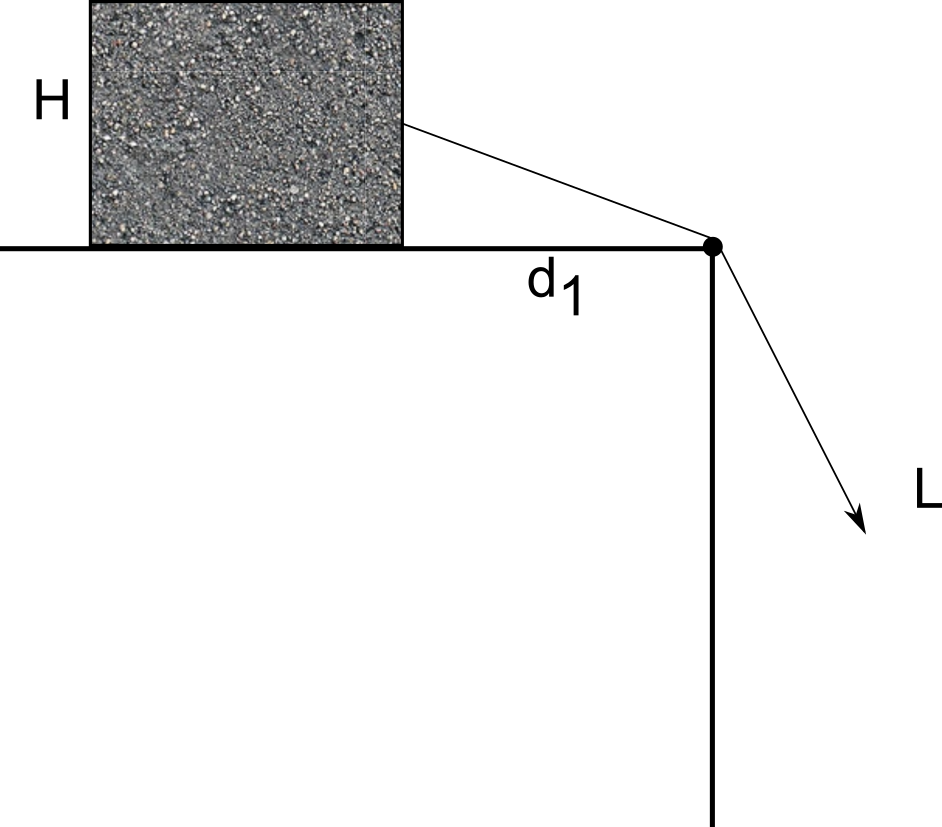
\includegraphics[width=7cm]{ink/week10/hangingBlocks}

  \begin{subproblem}
    \item Make a sketch of the free body diagram for the block.
      \vfill
    \item Determine the equations for Newton's Second Law in the $x$
      and $y$-directions.
      \vfill
      \clearpage
    \item Determine the equation for the acceleration in the
      horizontal direction. You should replace the trigonometric
      functions of the angle so that it only depends on $x$.
      \vfill
    \item Use the fact that $\frac{d}{dt} x(t) = v(t)$ to write the
      equation in the previous question as a system of two equations
      in terms of $v(t)$ and $x(t)$.
      \vfill

      \clearpage

    \item Divide the \textbf{time} that the block is sliding into
      steps of 0.05 seconds. Approximate the position of the object at
      any time using a Riemann sum. (Use a spreadsheet to make the
      approximations.)

      \clearpage

  \end{subproblem}

  \clearpage

\item Using the previous situation determine an approximation of the
  work done by the force of friction on the upper block from the start
  and until it reaches the corner.

  \vfill

\end{problem}

\postClass

\begin{problem}
\item Briefly state two ideas from today's class.
  \begin{itemize}
  \item
  \item
  \end{itemize}
\item
  \begin{subproblem}
    \item
  \end{subproblem}
\end{problem}

%=========================================================================
% Start of session on trig review
%=========================================================================
\preClass{Trig Review}

\qrcode[height=1.5cm,hyperlink,tight]{https://kellyblack.github.io/COMPASS/html/calcOne.html#goals-for-activity-28}

\begin{problem}
\item Determine the derivatives of each of the following functions:
  \begin{subproblem}
  \item $\sin(3t)$
    \vfill
  \item $\cos(3t)$
    \vfill
  \item $\tan(3t)$
    \vfill
  \item $\sin(t)\cos(t)$
    \vfill
  \end{subproblem}

  \clearpage

\item Determine the values of the missing lengths and angles of the
  triangles shown below.

  \scalebox{0.5}{%% Creator: Matplotlib, PGF backend
%%
%% To include the figure in your LaTeX document, write
%%   \input{<filename>.pgf}
%%
%% Make sure the required packages are loaded in your preamble
%%   \usepackage{pgf}
%%
%% Figures using additional raster images can only be included by \input if
%% they are in the same directory as the main LaTeX file. For loading figures
%% from other directories you can use the `import` package
%%   \usepackage{import}
%% and then include the figures with
%%   \import{<path to file>}{<filename>.pgf}
%%
%% Matplotlib used the following preamble
%%   \usepackage{fontspec}
%%   \setmainfont{Bitstream Vera Serif}
%%   \setsansfont{Bitstream Vera Sans}
%%   \setmonofont{Bitstream Vera Sans Mono}
%%
\begingroup%
\makeatletter%
\begin{pgfpicture}%
\pgfpathrectangle{\pgfpointorigin}{\pgfqpoint{8.000000in}{6.000000in}}%
\pgfusepath{use as bounding box, clip}%
\begin{pgfscope}%
\pgfsetbuttcap%
\pgfsetmiterjoin%
\definecolor{currentfill}{rgb}{1.000000,1.000000,1.000000}%
\pgfsetfillcolor{currentfill}%
\pgfsetlinewidth{0.000000pt}%
\definecolor{currentstroke}{rgb}{1.000000,1.000000,1.000000}%
\pgfsetstrokecolor{currentstroke}%
\pgfsetdash{}{0pt}%
\pgfpathmoveto{\pgfqpoint{0.000000in}{0.000000in}}%
\pgfpathlineto{\pgfqpoint{8.000000in}{0.000000in}}%
\pgfpathlineto{\pgfqpoint{8.000000in}{6.000000in}}%
\pgfpathlineto{\pgfqpoint{0.000000in}{6.000000in}}%
\pgfpathclose%
\pgfusepath{fill}%
\end{pgfscope}%
\begin{pgfscope}%
\pgfpathrectangle{\pgfqpoint{1.000000in}{0.600000in}}{\pgfqpoint{6.200000in}{4.800000in}} %
\pgfusepath{clip}%
\pgfsetbuttcap%
\pgfsetmiterjoin%
\pgfsetlinewidth{1.003750pt}%
\definecolor{currentstroke}{rgb}{0.000000,0.000000,0.000000}%
\pgfsetstrokecolor{currentstroke}%
\pgfsetdash{}{0pt}%
\pgfpathmoveto{\pgfqpoint{1.281818in}{3.000000in}}%
\pgfpathlineto{\pgfqpoint{4.100000in}{3.000000in}}%
\pgfpathlineto{\pgfqpoint{4.100000in}{4.745455in}}%
\pgfpathlineto{\pgfqpoint{1.281818in}{3.000000in}}%
\pgfusepath{stroke}%
\end{pgfscope}%
\begin{pgfscope}%
\pgfpathrectangle{\pgfqpoint{1.000000in}{0.600000in}}{\pgfqpoint{6.200000in}{4.800000in}} %
\pgfusepath{clip}%
\pgfsetbuttcap%
\pgfsetmiterjoin%
\pgfsetlinewidth{1.003750pt}%
\definecolor{currentstroke}{rgb}{0.000000,0.000000,0.000000}%
\pgfsetstrokecolor{currentstroke}%
\pgfsetdash{}{0pt}%
\pgfpathmoveto{\pgfqpoint{1.563636in}{0.818182in}}%
\pgfpathlineto{\pgfqpoint{4.100000in}{0.818182in}}%
\pgfpathlineto{\pgfqpoint{4.100000in}{2.345455in}}%
\pgfpathlineto{\pgfqpoint{1.563636in}{0.818182in}}%
\pgfusepath{stroke}%
\end{pgfscope}%
\begin{pgfscope}%
\pgfpathrectangle{\pgfqpoint{1.000000in}{0.600000in}}{\pgfqpoint{6.200000in}{4.800000in}} %
\pgfusepath{clip}%
\pgfsetrectcap%
\pgfsetroundjoin%
\pgfsetlinewidth{1.003750pt}%
\definecolor{currentstroke}{rgb}{0.000000,0.000000,0.000000}%
\pgfsetstrokecolor{currentstroke}%
\pgfsetdash{}{0pt}%
\pgfpathmoveto{\pgfqpoint{3.818182in}{3.000000in}}%
\pgfpathlineto{\pgfqpoint{3.818182in}{3.218182in}}%
\pgfpathlineto{\pgfqpoint{4.100000in}{3.218182in}}%
\pgfusepath{stroke}%
\end{pgfscope}%
\begin{pgfscope}%
\pgfpathrectangle{\pgfqpoint{1.000000in}{0.600000in}}{\pgfqpoint{6.200000in}{4.800000in}} %
\pgfusepath{clip}%
\pgfsetrectcap%
\pgfsetroundjoin%
\pgfsetlinewidth{1.003750pt}%
\definecolor{currentstroke}{rgb}{0.000000,0.000000,0.000000}%
\pgfsetstrokecolor{currentstroke}%
\pgfsetdash{}{0pt}%
\pgfpathmoveto{\pgfqpoint{3.818182in}{0.818182in}}%
\pgfpathlineto{\pgfqpoint{3.818182in}{1.036364in}}%
\pgfpathlineto{\pgfqpoint{4.100000in}{1.036364in}}%
\pgfusepath{stroke}%
\end{pgfscope}%
\begin{pgfscope}%
\pgftext[x=1.620000in,y=3.043636in,left,base]{\sffamily\fontsize{14.000000}{16.800000}\selectfont \(\displaystyle \pi/3\)}%
\end{pgfscope}%
\begin{pgfscope}%
\pgftext[x=3.818182in,y=3.741818in,left,base]{\sffamily\fontsize{14.000000}{16.800000}\selectfont \(\displaystyle 0.6\)}%
\end{pgfscope}%
\begin{pgfscope}%
\pgftext[x=1.338182in,y=4.527273in,left,base]{\sffamily\fontsize{20.000000}{24.000000}\selectfont A}%
\end{pgfscope}%
\begin{pgfscope}%
\pgftext[x=1.901818in,y=0.861818in,left,base]{\sffamily\fontsize{14.000000}{16.800000}\selectfont \(\displaystyle \theta\)}%
\end{pgfscope}%
\begin{pgfscope}%
\pgftext[x=2.747273in,y=0.861818in,left,base]{\sffamily\fontsize{14.000000}{16.800000}\selectfont \(\displaystyle 0.3\)}%
\end{pgfscope}%
\begin{pgfscope}%
\pgftext[x=2.550000in,y=1.690909in,left,base]{\sffamily\fontsize{14.000000}{16.800000}\selectfont \(\displaystyle 0.6\)}%
\end{pgfscope}%
\begin{pgfscope}%
\pgftext[x=1.450909in,y=2.345455in,left,base]{\sffamily\fontsize{20.000000}{24.000000}\selectfont B}%
\end{pgfscope}%
\end{pgfpicture}%
\makeatother%
\endgroup%
}

  \vfill

\end{problem}

\actTitle{Derivatives of Other Trigonometric Functions}
\begin{problem}

\item We examine the identity
  \begin{eqnarray*}
    \sin^2(\theta) + \cos^2(\theta) & = & 1.
  \end{eqnarray*}

  \begin{subproblem}
  \item Make a sketch of the unit circle. Use the definition of sine
    and cosine to explain why the identity above is true.
    \sideNote{Just give a heuristic explanation.}
    \vfill

  \item Divide both sides of the identity by $\cos^2(\theta)$.
    \vfill

  \item Use the definition of the tangent and secant to express the
    new result in terms of these two trigonometric functions.
    \vfill

  \end{subproblem}

  \clearpage

\item We derive the derivative of $\sec(\theta)$.

  \begin{subproblem}
    \item Express $\sec(\theta)$ as a function of the cosine.
      \vspace{4em}
    \item Determine the derivative of the previous expression.
      \vfill
    \item Use any appropriate trigonometric identity to simplify the
      expression.
      \vfill
  \end{subproblem}
  \clearpage

\item We derive the derivative of $\cot(\theta)$.

  \begin{subproblem}
  \item Express $\cot(\theta)$ as a function of the sine and the
    cosine.
    \vspace{4em}
    \item Determine the derivative of the previous expression.
      \vfill
    \item Use any appropriate trigonometric identity to simplify the
      expression.
      \vfill
  \end{subproblem}
  \clearpage

\end{problem}

\postClass

\begin{problem}
\item Briefly state two ideas from today's class.
  \begin{itemize}
  \item
  \item
  \end{itemize}
\item A person is standing at the origin, $(0,0)$, and they are facing
  in the positive $x$-direction. The person turns to the left
  $\frac{\pi}{3}$ radians, walks 3 meters in 10 seconds. The person
  stops, turns $\frac{\pi}{4}$ to the right and walks 5 meters in
  another 10 seconds.
  \begin{subproblem}
    \item  Make a sketch of the person's path.
      \vfill
    \item Determine the person's position at 10 and 20 seconds.
      \vfill
    \item Determine the person's position for any time less than 10
      seconds.
      \vfill
    \item Determine the person's position for any time between 10 and
      20 seconds.
      \vfill
  \end{subproblem}
  \clearpage
\item A person is standing at the origin, $(0,0)$, and they are facing
  in the positive $x$-direction. The person turns to the left
  $\frac{2\pi}{3}$ radians, walks 3 meters in 10 seconds. The person
  stops, turns $\frac{\pi}{2}$ to the left and walks 5 meters in
  another 10 seconds.
  \begin{subproblem}
    \item  Make a sketch of the person's path.
      \vfill
    \item Determine the person's position at 10 and 20 seconds.
      \vfill
    \item Determine the person's position for any time.
      \vfill
  \end{subproblem}
\end{problem}


%%% Local Variables:
%%% mode: latex
%%% TeX-master: "labManual"
%%% End:


%\chapter{Circular Motion}
%%=========================================================================
% Start of activity on simple harmonic motion.
%=========================================================================
\preClass{Derivatives of Basic Trigonometric Functions}

\qrcode[height=1.5cm,hyperlink,tight]{https://kellyblack.github.io/COMPASS/html/calcOne.html#goals-for-activity-29}

\begin{problem}
\item Determine the derivatives of the following functions:
  \begin{subproblem}
  \item $\sin(3t)$
    \vfill
  \item $\cos(8t)$
    \vfill
  \end{subproblem}
\item Determine the general anti-derivatives of the following functions:
  \begin{subproblem}
  \item $\cos(3t)$
    \vfill
  \item $\sin(8t)$
    \vfill
  \end{subproblem}

\clearpage

\item An object has an acceleration given by
  \begin{eqnarray*}
    a(t) & = & 2\sin(5t) + 5e^{-2t},
  \end{eqnarray*}
  and the initial velocity is $v_0$, and the initial position is $x_0$.
  \begin{subproblem}
  \item Determine the position at any time.
    \vfill
  \item Describe the qualitative behaviour of the object's
    position. Does the object's position oscillate, grow, or decay?
    For what values of $v_0$ and $x_0$ do you see different
    behaviours?
    \vfill
  \end{subproblem}

\end{problem}


\actTitle{Simple Harmonic Motion}
\begin{problem}

\item An object is attached to a rigid spring on a frictionless
  horizontal table. The origin is defined to be the equilibrium
  position for the object. The mass of the object is 3kg. The object
  is drawn back 0.05m and released from rest. The spring obeys Hooke's
  law, and it's constant is $k=0.4$N/m.
  \begin{subproblem}
    \item Make a sketch of the physical situation.
      \vfill
    \item Make a sketch of the free body diagram. Ignore any friction
      assuming that the friction is negligible for now.
      \vfill
    \item Describe the qualitative behaviour that you expect to see
      from the physical system. How should it behave? 
      \vfill
    \item Determine the equation of motion in the $x$-direction
      ignoring friction.
      \label{subproblem:odeMassSpring}
      \vfill

    \item Based on your description of the expected behaviour what
      kind of \textbf{functions} mimics that behaviour?
      \vspace{3em}

      \clearpage

    \item Assume that the solution has the form
      \begin{eqnarray*}
        x(t) & = & A \sin(\omega t) + B \cos(\omega t),
      \end{eqnarray*}
      where $A$, $B$, and $\omega$ are constants.
      \sideNote{It is not uncommon to just make a guess at a general
        form, and then check to see if your intuition is consistent
        with the equation.}
      \begin{subproblem}
      \item Determine the velocity and acceleration based on the
        definition of the position above.
        \vfill
      \item Substitute these results into your equation for the motion
        of the object you derived in question
        \ref{subproblem:odeMassSpring}.
        \vfill
        \clearpage
      \item Put all of the sines on one side of the equality and all
        of the cosines on the other side of the equality. What must be
        true about the left and right hand sides?
        \sideNote{Hint: It has to be true for \textbf{all} time!}
        \vspace{6em}
      \item Is it possible to determine values for the constants to
        satisfy the equation and the initial conditions? If so what
        are they?
        \sideNote{Hint: Yes.}
        \vfill
      \end{subproblem}

  \end{subproblem}
\end{problem}

\postClass

\begin{problem}
\item Briefly state two ideas from today's class.
  \begin{itemize}
  \item
  \item
  \end{itemize}
\item Determine the first and second derivatives of the following functions.
  \begin{subproblem}
  \item $8\sin(5t)$
    \vfill
  \item $23\cos(2t)$
    \vfill
  \item $8\sin(5t)+2\cos(5t)$
    \vfill
  \item $23\cos(2t)-14\sin(2t)$
    \vfill
  \end{subproblem}
  %\clearpage
  \item An object is attached to a rigid spring on a frictionless
    horizontal table. The origin is determined to be the equilibrium
    position for the object. The mass of the object is 4kg. The object
    is drawn back 0.1m and released from rest. The spring obeys Hooke's
    law with a constant, $k=0.5$N/m. Determine the position of the object
    at any time.
  \item An object is attached to a rigid spring on a frictionless
      horizontal table. The origin is determined to be the equilibrium
      position for the object. The mass of the object is 2kg. The object
      starts at the origin with an initial velocity of 3 m/sec.
      The spring obeys Hooke's law with a constant, $k=0.2$N/m.
      Determine the position of the object at any time.
\end{problem}

%=========================================================================
% Start of activity on finding optimal values of a parameter in SHM
%=========================================================================
\preClass{Simple Harmonic Motion}

\qrcode[height=1.5cm,hyperlink,tight]{https://kellyblack.github.io/COMPASS/html/calcOne.html#goals-for-activity-30}

\begin{problem}
\item Determine the solution to the following differential equations.
  \begin{subproblem}
  \item $x'' + 4 x  =  0$, $x(0)=0$, $v(0)=1$.
    \vfill
  \item $x'' + 8 x  =  0$, $x(0)=1$, $v(0)=0$.
    \vfill
  \end{subproblem}
\end{problem}


\actTitle{Optimization For Simple Harmonic Motion - Determining The System}
\begin{problem}
\item A spring mass system is to be constructed. The system will be
  assembled on a horizontal table, and friction is ignored.
  \begin{subproblem}
    \item Make a sketch of the physical situation.
      \vfill
    \item Make a sketch of the free body diagram.  Assume that the
      friction is negligible for now. Assume that the spring constant
      is $k$ N/m and the mass is $m$ 
      \vfill
    \item Describe the qualitative behaviour that you expect to see
      from the physical system. How should it behave?
      \vfill
    \item Determine the equation of motion ignoring friction.
      \vfill
  \end{subproblem}

  \clearpage

\item We now have the general equations of motion for a spring-mass
  system with parameters $k$ and $m$. The goal is to determine values
  of $k$ and $m$ so that the first time \textbf{after} $t=0$ the
  system will reach its maximum distance away from the origin in
  $t=0.1$ seconds. Assume that the object is first pulled 0.3 m from
  equilibrium and released from rest. What is the constraint for $k$
  and $m$?

  \vfill

\item The cost of the spring depends on $k$ and is $(1+k^2)$\$. The cost of
  the object depends on its mass and is ($m-2k)$\$. What is the
  total cost of building the system?

  \vspace{4em}

\item Formally express the cost and objective functions:
    \label{activity:optimization:spring}
    \begin{eqnarray*}
      \mathrm{Minimize:} & &  \\
      \mathrm{Constraint:} & &
    \end{eqnarray*}



\end{problem}


\postClass

\begin{problem}
\item Briefly state two ideas from today's class.
  \begin{itemize}
  \item
  \item
  \end{itemize}


\item Rewrite the system to optimize from this set of activities
  (question \ref{activity:optimization:spring}).
    \begin{eqnarray*}
      \mathrm{Minimize:} & &  \\
      \mathrm{Constraint:} & &
    \end{eqnarray*}
    \begin{subproblem}
    \item Make a sketch of the constraint.  \sideNote{ Be sure to
        label your axes and label all important points on your graph.}

      \vfill

    \item Add a sketch of the cost functions for various values of the
      cost. What is the general pattern? Make a prediction for the
      optimal values of $k$ and $m$.

      \vspace{3em}
    \end{subproblem}
\clearpage

\item Rewrite the system to optimze from this set of activities
  (question \ref{activity:optimization:spring}).
  \begin{eqnarray*}
    \mathrm{Minimize:} & &  \\
    \mathrm{Constraint:} & &
  \end{eqnarray*}

  \begin{subproblem}
  \item Analytically determine the optimal values of $k$ and $m$.
    \vfill
  \end{subproblem}
\end{problem}

%=========================================================================
% Start of activities on systems of equations
%=========================================================================
\preClass{Linearizations}

\qrcode[height=1.5cm,hyperlink,tight]{https://kellyblack.github.io/COMPASS/html/calcOne.html#goals-for-activity-31}

\begin{problem}
\item We examine the linearization of the function
  \begin{eqnarray*}
    f(x) & = & x^2-4.
  \end{eqnarray*}
  \begin{subproblem}
  \item Draw a set of axes where $-2\leq x \leq 2$.

    \sideNote{ Be sure to label your axes and label all important
      points on your graph.}

    \vfill

  \item Make a sketch of the function $f(x)$ on the axes.
  \item Add a sketch of the tangent line to the function at $x=1$.
  \item Determine the formula for the tangent line at $x=1$.
    \sideNote{Another term for the tangent line is the
      \textit{linearization}. The function you just found is the
      linearization of $f(x)$ at $x=1$.}
    \vfill

    (over)
  \end{subproblem}
  \clearpage
\item Determine the linearization of the function
  \begin{eqnarray*}
    g(t) & = & \cos(t)
  \end{eqnarray*}
  at $t=\frac{\pi}{4}$.
\end{problem}


\actTitle{Approximating Solutions to Nonlinear Equations}
\begin{problem}
\item We will examine a way to determine an estimate for the value of
  $x$ that satisfies $0=x^2-4$.
  \begin{subproblem}
  \item Draw a set of axes where $-2\leq x \leq 2$.

    \sideNote{ Be sure to label your axes and label all important
      points on your graph.}

    \vfill

  \item Make a sketch of the relationship $f(x)=x^2-4$ on the axes.
  \item Suppose you cannot determine the value of $x$ where $f(x)=0$,
    but you estimate that $x=1$ is close to a root. Add a sketch of
    the tangent line to the function at $x=1$.

  \item Mark the point where the height of the graph of the
    \textbf{tangent line} is zero. Is this new $x$ value a better or
    worse approximation for the value of the actual root?

    \vspace{2em}

    \clearpage


  \item Determine analytically the equation for the tangent line to
    the graph of the curve at the initial estimate for the root,
    $x=1$. Determine the value of $x$ where the height of the graph of
    the tangent line is zero.

    \vfill


  \item Add sketch of another tangent line at the new value of $x$ to
    your original plot on the previous page.

  \item Mark the point where the height of the \textbf{tangent line}
    is zero. Is this new $x$ value a better or worse approximation for
    the value of $x$?

    \vspace{2em}

  \item Determine analytically the tangent line to the graph of the
    curve at the new estimate for the root. Determine the value of $x$
    where the height of the graph of this new tangent line is zero.

    \vfill


  \item Add sketch of another tangent line at the new value of $x$ to
    your original plot on the previous page.

  \item Mark the point where the height of the graph of the
    \textbf{new tangent line} is zero. Is this new $x$ value a better
    or worse approximation for the value of $x$?


  \end{subproblem}

  \clearpage

\item Determine an algorithm to calculate the tangent line to a
  function at $x=a$, and find the value of $x$ where the height of the
  graph of the tangent line is zero.

  \vfill

\clearpage

\item Use your algorithm multiple times to find an approximation to
  the square root of 4 with an initial estimate of $x=1$.

  \vfill

\item How do you know when to stop applying the algorithm and your
  approximation is ``close?''

\end{problem}


\postClass

\begin{problem}
\item Briefly state two ideas from today's class.
  \begin{itemize}
  \item
  \item
  \end{itemize}
\item Graphically determine the values of $x$ and $y$ that satisfy
  both of the following equations:
  \begin{eqnarray*}
    x^2 + y  & = & 0, \\
    x - 2y^2 & = & 1.
  \end{eqnarray*}

  \begin{subproblem}
  \item Draw a set of axes where $-3\leq x \leq 3$ and $-3 \leq y \leq
    3$.

    \sideNote{ Be sure to label your axes and label all important
      points on your graph.}

    \vfill

  \item Make a sketch of the relationship $x^2+y=0$ on the axes.
  \item Make a sketch of the relationship $x-2y^2=1$ on the axes.
  \item Circle and estimate the points where both relationships are
    satisfied.
  \end{subproblem}
\clearpage
\item Determine the values of $x$ and $y$ that satisfy both of the
  following equations:
  \begin{eqnarray*}
    x + 4y & = & 7, \\
    x + 3y & = & 5.
  \end{eqnarray*}
  Solve the system analytically.
  \clearpage
\item Graphically determine the values of $x$ and $y$ that satisfy
  both of the following equations:
  \begin{eqnarray*}
    x + 4y & = & 7, \\
    x + 3y & = & 5.
  \end{eqnarray*}
  \begin{subproblem}
  \item Draw a set of axes where $-3\leq x \leq 3$ and $-3 \leq y \leq
    3$.

    \sideNote{ Be sure to label your axes and label all important
      points on your graph.}

    \vfill

  \item Make a sketch of the relationship $x+4y=7$ on the axes.
  \item Make a sketch of the relationship $x+3y=5$ on the axes.
  \item Circle and estimate the points where both relationships are
    satisfied.
  \end{subproblem}
\end{problem}

%=========================================================================
% Start of activity on vector operations
%=========================================================================
\preClass{Law of Cosines}

\qrcode[height=1.5cm,hyperlink,tight]{https://kellyblack.github.io/COMPASS/html/calcOne.html#goals-for-activity-32}

\begin{problem}
\item Answer each of the questions below.

  \begin{subproblem}
  \item What is the value of $\cos(\theta)$ given $a$, $b$, and $c$
    for the triangle in the diagram below?

    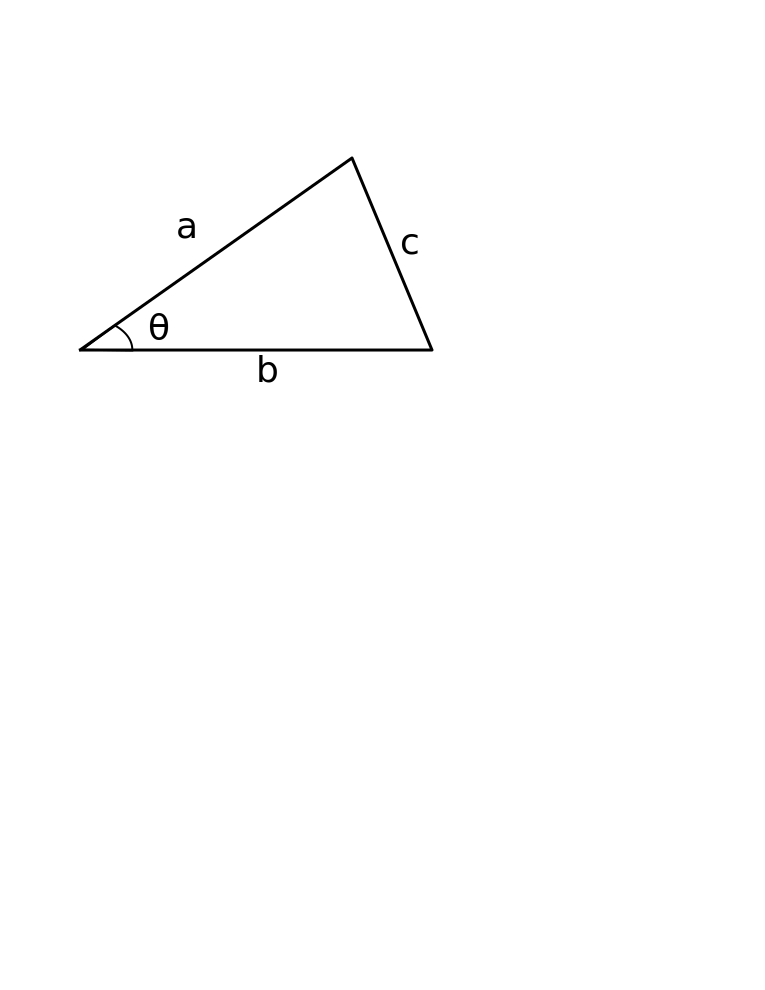
\includegraphics[width=5cm]{ink/week11/lawOfCosines}

  \item Determine the magnitude of the vector
    \begin{eqnarray*}
      \vec{u} & = & u_1 \vec{\imath} + u_2 \vec{\jmath}.
    \end{eqnarray*}

    \vfill

  \item Determine the magnitude of the vector
    \begin{eqnarray*}
      \vec{v} & = & v_1 \vec{\imath} + v_2 \vec{\jmath}.
    \end{eqnarray*}

    \vfill

  \item Determine the magnitude of the vector $\vec{u}-\vec{v}$ using
    the components as described above.
    \sideNote{Determine the components of $\vec{u}-\vec{v}$ and do not
      forget to FOIL out the terms when you determine the magnitude.}

    \vfill

  \end{subproblem}

\end{problem}


\actTitle{The Dot Product}
\begin{problem}
\item  In the diagram below sketch the vector $\vec{u}-\vec{v}$.

  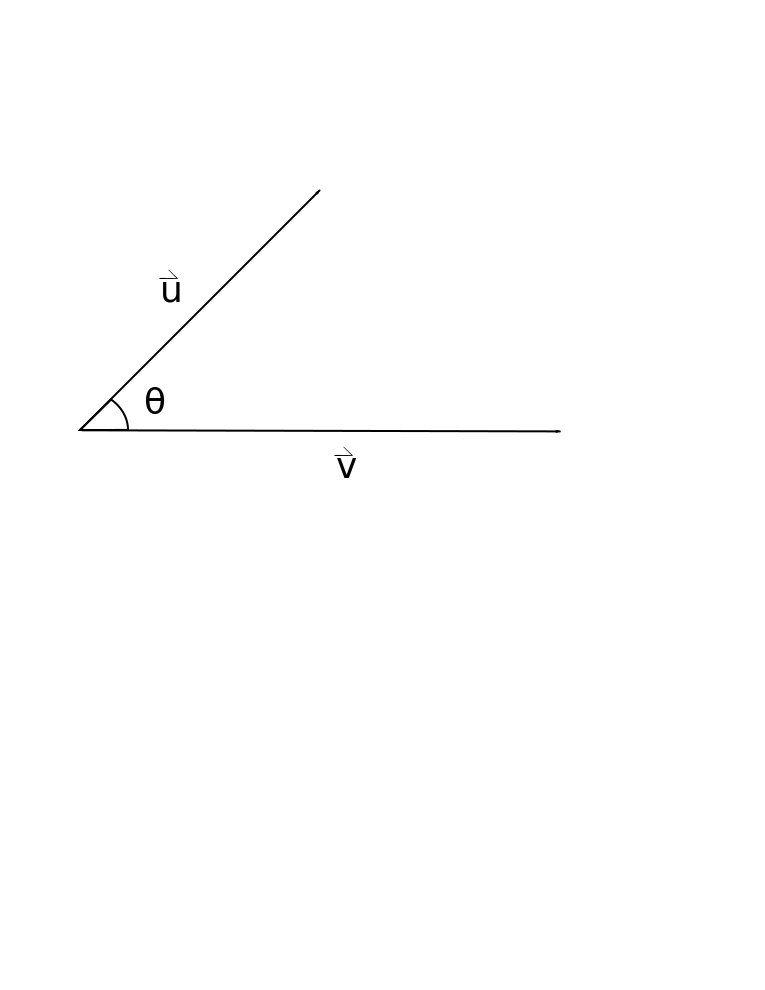
\includegraphics[width=7cm]{ink/week11/dotProduct}

\item Using your results from the pre-class work determine the value
  of
  \begin{eqnarray*}
    \| \vec{u} \| \| \vec{v} \| \cos(\theta)
  \end{eqnarray*}
  in terms of $\|\vec{u}\|$, $\|\vec{v}\|$, and $\|\vec{u}-\vec{v}\|$.

  \vfill

\item Substitute the components for $\vec{u}$ and $\vec{v}$ and
  simplify the expression as much as possible.

  \vfill

\clearpage

\item Determine the component of
  \begin{eqnarray*}
    \vec{u} & = & 5 \vec{\imath} + 3 \vec{\jmath}
  \end{eqnarray*}
  in the direction of
  \begin{eqnarray*}
    \vec{v} & = & \vec{\imath} + 2 \vec{\jmath}.
  \end{eqnarray*}

  \begin{subproblem}
  \item Make a sketch of the two vectors. (Make it big.)
    \vfill
  \item Draw the components on your sketch above.
  \item Calculate the length of the component of $\vec{u}$ in the
    direction of $\vec{v}$.
    \vfill
  \end{subproblem}

\end{problem}


\postClass

\begin{problem}
\item Briefly state two ideas from today's class.
  \begin{itemize}
  \item
  \item
  \end{itemize}
\item
  \begin{subproblem}
    \item
  \end{subproblem}
\end{problem}


%=========================================================================
% Start of activity on the cross product
%=========================================================================
\preClass{The Area of a Parallelogram}

\begin{problem}
\item Determine the area of the parallelogram shown below. The area
  should be in terms of $a$, $b$, and $\theta$.

  \includegraphics[width=5cm]{ink/week11/parallelogram}

  \vfill

\item Expand the expression
  \begin{eqnarray*}
    \left( a + b \right) \cdot \left( c + d \right).
  \end{eqnarray*}
  \sideNote{FOIL out the product.}

  \vfill

\end{problem}


\actTitle{The Cross Product}
\begin{problem}
\item A new operation, the cross product, is defined, and the
  operations to calculate the cross product are derived. The cross
  product of two vectors, $\vec{u}\times\vec{v}$, is derived by first
  defining the following identities:
  \begin{eqnarray*}
    \vec{\imath} \times \vec{\jmath} & = & \vec{k}, \\
    \vec{\jmath} \times \vec{k} & = & \vec{\imath}, \\
    \vec{k} \times \vec{\imath} & = & \vec{\jmath}, \\
    \vec{u} \times \vec{u} & = & 0 \vec{\imath}, \\
    \vec{u} \times \vec{v} & = & - \vec{v} \times \vec{u}.
  \end{eqnarray*}
  Note that the cross product of two vectors is a vector.
  \begin{subproblem}
  \item For the first three identities above make a sketch to
    demonstrate the relationships.
    \vfill

    \clearpage

  \item Suppose that
    \begin{eqnarray*}
      \vec{u} & = & u_1 \vec{\imath} + u_2 \vec{\jmath}
    \end{eqnarray*}
    and
    \begin{eqnarray*}
      \vec{v} & = & v_1 \vec{\imath} + v_2 \vec{\jmath}.
    \end{eqnarray*}
    Use the definitions above and assume that the cross product obeys
    the distributive rule to derive a general formula for the cross
    product.
    \vfill
    \vfill

  \item Determine the cross product of $2 \vec{\imath} + 2\vec{\jmath}$ and $4 \vec{\imath}$.
    \vfill

    \clearpage

  \item Suppose that
    \begin{eqnarray*}
      \vec{u} & = & u_1 \vec{\imath} + u_2 \vec{\jmath} + u_3 \vec{k}
    \end{eqnarray*}
    and
    \begin{eqnarray*}
      \vec{v} & = & v_1 \vec{\imath} + v_2 \vec{\jmath} + v_3 \vec{k}.
    \end{eqnarray*}
    Use the definitions above and assume that the cross product obeys
    the distributive rule to derive a general formula for the cross product.
    \vfill

  \end{subproblem}
\end{problem}


\postClass

\begin{problem}
\item Briefly state two ideas from today's class.
  \begin{itemize}
  \item
  \item
  \end{itemize}
\item
  \begin{subproblem}
    \item
  \end{subproblem}
\end{problem}


%=========================================================================
% Start of activity on motion in a circle
%=========================================================================
\preClass{Path Around The Unit Circle}

\begin{problem}
\item Suppose that the position of a point mass is given by
  \begin{eqnarray*}
    \vec{r}(t) & = & \cos(t) \vec{\imath} + \sin(t) \vec{\jmath}.
  \end{eqnarray*}
  \begin{subproblem}
  \item Determine the position of the point mass at ${\displaystyle
      t=\frac{\pi}{3}}$.
    \sideNote{Your answer should be a vector using
      $\vec{\imath}-\vec{\jmath}$ notation.}
    \vfill
  \item Determine the position of the point mass at ${\displaystyle
      t=\frac{\pi}{4}}$.
    \vfill
  \item Determine the position of the point mass at ${\displaystyle
      t=\frac{2\pi}{3}}$.
    \vfill
  \item Determine the position of the point mass at ${\displaystyle
      t=\frac{\pi}{2}}$.
    \vfill
    (over)
    \clearpage
  \item Make a sketch of all the points that the point mass moves
    through from $t=0$ to $t=2\pi$. (Mark the starting point and the
    direction of movement.)
    \vfill
  \end{subproblem}
\end{problem}


\actTitle{Angular Velocity}
\begin{problem}
\item Suppose that the position of a point mass is given by
  \begin{eqnarray*}
    \vec{r}(t) & = & R\cos(\theta(t)) \vec{\imath} + R\sin(\theta(t)) \vec{\jmath},
  \end{eqnarray*}
  where $R$ is a constant and $\theta(t)$ is a function of time.
  \label{activity:angularVelocity:one}
  \begin{subproblem}
  \item What can you say about the position of the point mass?
    \vfill
  \item What is the magnitude of the position for any time?
    \vfill
  \item What is the velocity of the point mass in terms of $\theta(t)$
    and $\theta'(t)$.
    \vfill
  \item What is the magnitude of the velocity for any time?
    \vfill
  \end{subproblem}

  \clearpage

\item Assume that a point mass is located on the edge of a circle with
  radius $R$.  From the definition of radian measure the length of the
  corresponding arc of a circle is given by
  \begin{eqnarray*}
    s & = & R \theta(t).
  \end{eqnarray*}
  \label{activity:angularVelocity:two}
  \begin{subproblem}
  \item Assume that $R$ is a constant. Determine the speed of the
    point mass at any time.
    \vfill
  \item How do you interpret the meaning of $\theta'(t)$?
    \vfill
  \item Assume that $R$ is a constant. Determine the acceleration of
    the point mass at any time.
    \vfill
  \end{subproblem}

\clearpage

\item Assume that the point masses in questions
  \ref{activity:angularVelocity:one} and
  \ref{activity:angularVelocity:two} above have mass $m$ kg. In both
  cases determine the kinetic energy of the point masses.

\end{problem}


\postClass

\begin{problem}
\item Briefly state two ideas from today's class.
  \begin{itemize}
  \item
  \item
  \end{itemize}
\item
  \begin{subproblem}
    \item
  \end{subproblem}
\end{problem}



%=========================================================================
% Start of activity on riemann sums and moment of intertia
%=========================================================================
\preClass{Moment of Inertia}

\begin{problem}
\item A point mass of 2 kg is located at $3\vec{i} + 2\vec{j}$, and a
  point mass of 4 kg is located at $-\vec{i}+3\vec{j}$. The two masses
  rotate around the $\vec{k}$ axis at the same rate. Determine the
  moment of inertia of the two masses.

  \vfill

  (over)
  \clearpage


\item Three point masses are lined up on the $x$ axis. They are
  positioned at $x_n=\frac{n}{3}$ where $n=0,~1,~2$. The mass of each
  point mass is $\frac{5n}{3}$ kg.
  \begin{subproblem}
    \item Make a rough sketch of the system.
      \vfill
    \item Determine the center of mass of the system.
      \vfill
    \item Determine the moment of inertia of the system around the
      $y$-axis.
      \vfill
  \end{subproblem}


\end{problem}


\actTitle{Moment of Inertia for Continuous Masses}
\begin{problem}
\item A thin metal rod is aligned along the $x$-axis. The left side of
  the rod is located at $x=0$m and the right hand side is located at
  $x=1$m. The density of the rod is $\rho(x)=5x$ kg/m.
  \begin{subproblem}
    \item Make a rough sketch of the system.
      \vfill
    \item Divide the rod into $N$ equal sized small
      segments. Determine the location of the left hand side of each
      small segment.
      \vfill
    \item Determine an approximation for the density of each small
      segment. (Keep the approximation in terms of $x_k$.)
      \vfill
    \item Determine the approximate mass and the moment of inertia
      around the $y$-axis for each small segment.
      \vfill

      \clearpage

    \item Determine the sum that can be used to approximate the center
      of mass and the sum that can be used to approximate the moment
      of inertia of the whole rod around the $y$-axis.

      \vfill

    \item Determine the exact center of mass and moment of inertia for
      the rod.

      \vfill
      \vfill

  \end{subproblem}
\end{problem}

\postClass

\begin{problem}
\item Briefly state two ideas from today's class.
  \begin{itemize}
  \item
  \item
  \end{itemize}
\item Relate the sum for the center of mass with the integral. Make a
  plot and discuss the relationship with the sum with the area under a
  function. (Which function are you finding the area under?)

  \vfill
\end{problem}


%=========================================================================
% Start of day on moment of inertia and angular momentum.
%=========================================================================
\preClass{Constant Angular Velocity}

\begin{problem}
\item An object moves around a circle with a constant angular
  velocity, $\omega$, and the distance from the origin is $r$. The
  initial angle, $\theta$, from the $x$-axis is zero.
  \begin{subproblem}
  \item Determine the angle at any time.
    \vfill
  \item Determine the position at any time.
    \sideNote{Use proper vector notation.}
    \vfill
  \item Determine the derivative of the position at any time.
    \vfill
  \item What is the magnitude of the velocity vector?
    \vfill
  \item Determine the derivative of the velocity at any time.
    \vfill
  \end{subproblem}

  \clearpage

\item An object moves around a circle of radius $r$  at a constant
  rate, $\theta=\omega t$. Its position at any time is $\vec{r}$.

  \begin{subproblem}
    \sideNote{Draw the vector $\delta\vec{r}$ in the plot.}
  \item Graphically represent the difference in the positions between
    any times, $\vec{r}(t+\delta t)-\vec{r}(t)$. Blow up, redraw, and
    focus just on the two positions shown on the circle.

\begin{tikzpicture}[y=2.2cm, x=2.2cm,font=\sffamily]
  \draw[black,->] (-1.5,0) -- (1.5,0) node[anchor=north east] {$x$};
  \draw[black,->] (0,-1.5) -- (0,1.5) node[anchor=north east] {$y$};
  \draw[black,thick] (0,0) circle [radius=1];
  \fill[black,shift={+(55:1)}] (0,0) circle [radius=0.025];
  \fill[black,shift={+(65:1)}] (0,0) circle [radius=0.025];
  \draw[black,->,ultra thick] (0,0) -- +(55:1) node[anchor=west,shift={(0.15,-0.05)}] {$\vec{r}(t)$};
  \draw[black,->,ultra thick] (0,0) -- +(65:1) node[anchor=west,shift={(0,0.2)}] {$\vec{r}(t+\triangle t)$};
\end{tikzpicture}
    \vfill

  \item Graphically represent the difference in the velocity vectors,
    $\vec{v}(t+\delta t)-\vec{v}(t)$, at the two positions in the plot
    below. Blow up, redraw, and focus just on the two positions on the
    circle.
    \sideNote{Based on your previous result estimate the velocity vectors.}

    \begin{tikzpicture}[y=2.2cm, x=2.2cm,font=\sffamily]
      \draw[black,->] (-1.5,0) -- (1.5,0) node[anchor=north east] {$x$};
      \draw[black,->] (0,-1.5) -- (0,1.5) node[anchor=north east] {$y$};
      \draw[black,thick] (0,0) circle [radius=1];
      \fill[black,shift={+(55:1)}] (0,0) circle [radius=0.025];
      \fill[black,shift={+(65:1)}] (0,0) circle [radius=0.025];
      \draw[black,->,ultra thick] (0,0) -- +(55:1) node[anchor=west,shift={(0.15,-0.05)}] {$\vec{r}(t)$};
      \draw[black,->,ultra thick] (0,0) -- +(65:1) node[anchor=west,shift={(0,0.2)}] {$\vec{r}(t+\triangle t)$};
    \end{tikzpicture}

    \vfill

  \end{subproblem}

\end{problem}


\actTitle{Energy Associated With Constant Angular Velocity}
\begin{problem}
\item An object moves around a circle of radius $r$ at a constant
  rate, $\theta=\omega t$. Its position at any time is denoted
  $\vec{r}(t)$.

  \begin{subproblem}
  \item Determine the position at any time. Express the position as
    a vector.
    \sideNote{Assume that $\omega$ is constant.} %\\
    %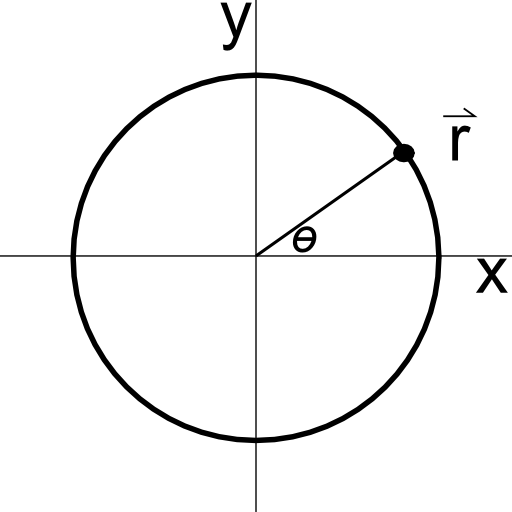
\includegraphics[width=7cm]{ink/week12/circularMotion}
    \vfill
  \item Determine the velocity and the acceleration by taking the
    derivatives of the position with respect to time.
    \vfill
  \item Determine the kinetic energy of the object at any time.
    \sideNote{Is the kinetic energy a vector or scalar quantity?}
    \vfill
  \end{subproblem}

  \clearpage

\item An object whose position is given by $\vec{r}(t)$ is moving in
  two dimensions. The angle between the velocity and the position is
  $\gamma$ as shown in the diagram below. The velocity can be
  expressed by two components, one in the direction of the position
  vector and the other direction
  perpendicular to the position vector. \\
  \begin{tikzpicture}[y=2.8cm, x=2.8cm,font=\sffamily]
    \draw[black,->] (-0.2,0) -- (1.5,0) node[anchor=north east] {$x$};
    \draw[black,->] (0,-0.2) -- (0,1.5) node[anchor=north east] {$y$};
    \draw[black,->,ultra thick] (0,0) -- +(55:1.3) node[midway,above,shift={(-0.05,0.05)}] {$\vec{r}(t)$};
    \draw[black,->] (55:1.35) -- +(55:0.65);
    \draw[black,->] (55:1.35) -- +(-35:0.25);
    \draw[black,->] (55:1.35) -- +(35:0.7) node[anchor=west,shift={(0.0,0.0)}] {$\vec{v}(t)$};
    \node at (53:1.7) {$\gamma$};
    \draw (55:1.35) ++(35:0.2) arc(35:43:0.5);
  \end{tikzpicture}

  \begin{subproblem}
  \item Determine the magnitude of the component of the velocity that
    is parallel to the position vector and the magnitude of the
    component of the velocity that is perpendicular to the position
    vector. Your answer should be in terms of the magnitude of
    $\vec{v}$ and the angle between the vectors, $\gamma$.

    \vfill

  \item Determine the magnitude of the vector given by
    $\vec{r}\times\vec{v}$.

    \vfill

  \item Determine the value of $\vec{r}\cdot\vec{v}$ in terms of the
    magnitude of the position and velocity vectors.

    \vfill

  \item Determine the magnitude of the component of the velocity that
    is parallel to the position vector and the magnitude of the
    component of the velocity that is perpendicular to the position
    vector in terms of the dot and cross products above.

    \vfill

  \end{subproblem}
  \clearpage
\item An object moves around a circle of radius $r$  at a constant
  rate, $\theta=\omega t$. Its position at any time is $\vec{r}$.
  \begin{subproblem}
  \item Determine $\vec{r}\times\vec{v}$ and the magnitude of the
    result.

    \vfill

  \item Determine  $\vec{r}\cdot\vec{v}$.

    \vfill

  \item What do these two results imply about the relationship between
    the position and velocity vectors?

    \vfill

  \end{subproblem}
\end{problem}

\postClass

\begin{problem}
\item Briefly state two ideas from today's class.
  \begin{itemize}
  \item
  \item
  \end{itemize}
\item for each image below make a rough sketch of the missing
  component, $\vec{r}$, $\vec{v}$, or $\vec{\omega}$.
  \begin{subproblem}
  \item 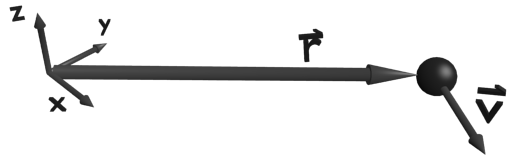
\includegraphics[width=7cm]{blender/week12/negativeZOmega}
  \item 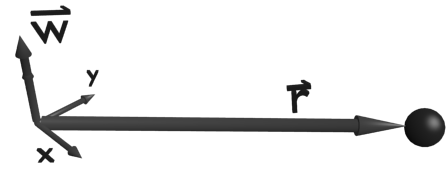
\includegraphics[width=7cm]{blender/week12/findOmega}
  \item 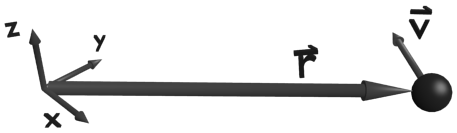
\includegraphics[width=7cm]{blender/week12/positiveZOmega}
  \end{subproblem}
\end{problem}


%=========================================================================
% Start of activity on angular velocity for simple and non-simple
% harmonic motion.
%=========================================================================
\preClass{Constant Angular Velocity}

\begin{problem}
%\item A mass is moving in a circle of radius $R$ at a constant speed,
%  $v$.
%  \begin{subproblem}
%  \item Draw a picture of the path and include the free body diagram.
%    \vfill
%  \item Add the acceleration of the object in your plot above. In
%    which direction is the acceleration?
%    \vfill
%  \item What is the magnitude of the acceleration?
%    \vfill
%  \item How will the diagram change if the velocity is not constant?
%    \vfill
%  \end{subproblem}
%
%\clearpage

\item The position of a mass is
  $\vec{r}(t)=r\cos(\omega t)\vec{i}+r\sin(\omega t)\vec{j}$. The
  value of $\omega$ is a positive constant.
  \begin{subproblem}
  \item Draw a sketch of the object's path. Include the start point
    and the direction of travel of the object.
    \vfill
  \item How long does it take to complete one full revolution?
    \vspace{3em}
  \item Determine the velocity and acceleration. Add a sketch of the
    vectors to your plot above.
    \vfill
    \clearpage
  \item Determine the value of $|\vec{a}(t)|$ using your results for
    the velocity and acceleration above.
    \vfill
  \item Determine the value of $\frac{|\vec{v}(t)|^2}{|\vec{r}(t)|}$
    using your results for the velocity and acceleration above.
    \vfill
  \end{subproblem}

\end{problem}

\actTitle{Non-constant Angular Velocity}
\begin{problem}
\item The position of a mass is
  $\vec{r}(t)=r\cos(\omega t^2)\vec{i}+r\sin(\omega t^2)\vec{j}$. The
  parameter $\omega$ is a constant.
  \begin{subproblem}
  \item Draw a sketch of the object's path. Include the start point
    and the direction of travel of the object.
    \vfill
  \item Determine the velocity and acceleration. Add a sketch of the
    vectors to your plot above.
    \vfill
    \clearpage
  \item Is the relationship $|\vec{a}|=\frac{|\vec{v}(t)|^2}{|\vec{r}(t)|}$
    still true?
    \vfill
    \vfill
  \item Determine the radial component, $\vec{a}_r(t)$, of the
    acceleration.
    \vfill
  \item Show that $|\vec{a}_r(t)| = \frac{|\vec{v}(t)|^2}{|\vec{r}(t)|}$
    \vfill
  \end{subproblem}
\end{problem}

\postClass

\begin{problem}
\item Briefly state two ideas from today's class.
  \begin{itemize}
  \item
  \item
  \end{itemize}
\item The position of a mass is
  $\vec{r}(t)=r\cos(\omega t)\vec{i}+r\sin(\omega t)\vec{j}$. The
  parameter $\omega$ is a constant.
  \begin{subproblem}
  \item Draw a sketch of the object's path. Include the start point
    and the direction of travel of the object.
    \vfill
    \vfill
  \item Find the distance that the mass travels from time $t=0$ to a
    later time, $t=T$.
    \vfill
  \item What happens as the value of $\omega$ changes? For example
    if you double $\omega$ what happens to the distance? What does
    that imply about the speed?
    \vfill
  \end{subproblem}
\end{problem}


%=========================================================================
% Start of day on the derivative of inverse functions
%=========================================================================
\preClass{Inverse Trigonometric Functions}

\begin{problem}
\item Make a sketch of the unit circle. Mark and label the points on
  the circle that correspond to the angles $\frac{\pi}{4}$,
  $\frac{\pi}{3}$, and $\frac{3\pi}{4}$.
  \sideNote{Label the angle as well as the points on the edge of the circle.}
  \vfill
  \vfill
\item If the sine of an angle is $\frac{\sqrt{2}}{2}$ what are all
  possible values of the angle?
  \vfill
\item If the sine of an angle is $\frac{\sqrt{3}}{2}$ what are all
  possible values of the angle?
  \vfill
\item Is the sine function invertable? (Briefly explain your
  reasoning.)
  \vspace{2em}
\end{problem}


\actTitle{The Derivative of the Inverse of a Function}
\begin{problem}
\item Suppose that
  \begin{eqnarray}
    \label{eqn:arcsin}
    y &= & \arcsin(t),
  \end{eqnarray}
  and assume that $y$ is between $\frac{-\pi}{2}$ and $\frac{\pi}{2}$ and
  $t$ is between -1 and 1.
  \begin{subproblem}
  \item Solve equation \ref{eqn:arcsin} for $t$ as a function of
    $y$.
    \label{subproblem:inverseSine}
    \vfill
  \item Assuming that $y$ is a function of $t$ use the chain rule to
    determine the derivative of $y(t)$ with respect to $t$.
    \vfill
  \item Use the identity $\sin^2(y)+\cos^2(y)=1$ to express your
    equation for $y'(t)$ in terms of $\sin(y)$.
    \vfill
  \item Use the definition of $y(t)$ from part
    \ref{subproblem:inverseSine} to determine $y'(t)$ only in terms of
    $t$.
    \vfill

  \end{subproblem}

  \clearpage

\item Suppose that
  \begin{eqnarray}
    \label{eqn:inverseFunction}
    y &= & f^{-1}(t).
  \end{eqnarray}
  \begin{subproblem}
  \item Solve equation \ref{eqn:inverseFunction} for $t$ as a function
    of $y$.
    \label{subproblem:generalInverse}
    \vfill

  \item Assuming that $y$ is a function of $t$ use the chain rule to
    determine the derivative of $y(t)$.
    \vfill

  \item Use the definition of $y(t)$ from equation (\ref{eqn:inverseFunction}) to determine $y'(t)$ only in terms of $t$.
    \vfill

  \end{subproblem}


\end{problem}

\postClass

\begin{problem}
\item Briefly state two ideas from today's class.
  \begin{itemize}
  \item
  \item
  \end{itemize}

\item Use the method to determine the derivative of the inverse to
  show that the derivative of the square root function satisfies
  \begin{eqnarray*}
    \frac{d}{dt} \sqrt{t} & = & \frac{1}{2\sqrt{t}}.
  \end{eqnarray*}

  \vfill

\item Use the method to determine the derivative of the inverse to
  \textbf{derive} the derivative of the inverse cosine function.
  \vfill

\item Use the method to determine the derivative of the inverse to
  show that the derivative of the natural logarithm satisfies
  \begin{eqnarray*}
    \frac{d}{dt} \ln(t) & = & \frac{1}{t}.
  \end{eqnarray*}

  \vfill


\end{problem}




%%% Local Variables:
%%% mode: latex
%%% TeX-master: "labManual"
%%% End:


\chapter{GNU Free Documentation License}

\hfuzz = .6pt % avoid black boxes
           
%---------------------------------------------------------------------
%\chapter*{\rlap{GNU Free Documentation License}}
%\phantomsection  % so hyperref creates bookmarks
%\addcontentsline{toc}{chapter}{GNU Free Documentation License}
%\label{label_fdl}

 \begin{center}

       Version 1.3, 3 November 2008


 Copyright \copyright{} 2000, 2001, 2002, 2007, 2008  Free Software Foundation, Inc.
 
 \bigskip
 
     \texttt{<http://fsf.org/>}
  
 \bigskip
 
 Everyone is permitted to copy and distribute verbatim copies
 of this license document, but changing it is not allowed.
\end{center}


%\begin{center}
\noindent
{\bf\normalsize Preamble}
%\end{center}

The purpose of this License is to make a manual, textbook, or other
functional and useful document ``free'' in the sense of freedom: to
assure everyone the effective freedom to copy and redistribute it,
with or without modifying it, either commercially or noncommercially.
Secondarily, this License preserves for the author and publisher a way
to get credit for their work, while not being considered responsible
for modifications made by others.

This License is a kind of ``copyleft'', which means that derivative
works of the document must themselves be free in the same sense.  It
complements the GNU General Public License, which is a copyleft
license designed for free software.

We have designed this License in order to use it for manuals for free
software, because free software needs free documentation: a free
program should come with manuals providing the same freedoms that the
software does.  But this License is not limited to software manuals;
it can be used for any textual work, regardless of subject matter or
whether it is published as a printed book.  We recommend this License
principally for works whose purpose is instruction or reference.


%\begin{center}
\noindent
{\normalsize\bf 1. APPLICABILITY AND DEFINITIONS\par}
\phantomsection
%\addcontentsline{toc}{section}{1. APPLICABILITY AND DEFINITIONS}
%\end{center}

This License applies to any manual or other work, in any medium, that
contains a notice placed by the copyright holder saying it can be
distributed under the terms of this License.  Such a notice grants a
world-wide, royalty-free license, unlimited in duration, to use that
work under the conditions stated herein.  The ``\textbf{Document}'', below,
refers to any such manual or work.  Any member of the public is a
licensee, and is addressed as ``\textbf{you}''.  You accept the license if you
copy, modify or distribute the work in a way requiring permission
under copyright law.

A ``\textbf{Modified Version}'' of the Document means any work containing the
Document or a portion of it, either copied verbatim, or with
modifications and/or translated into another language.

A ``\textbf{Secondary Section}'' is a named appendix or a front-matter section of
the Document that deals exclusively with the relationship of the
publishers or authors of the Document to the Document's overall subject
(or to related matters) and contains nothing that could fall directly
within that overall subject.  (Thus, if the Document is in part a
textbook of mathematics, a Secondary Section may not explain any
mathematics.)  The relationship could be a matter of historical
connection with the subject or with related matters, or of legal,
commercial, philosophical, ethical or political position regarding
them.

The ``\textbf{Invariant Sections}'' are certain Secondary Sections whose titles
are designated, as being those of Invariant Sections, in the notice
that says that the Document is released under this License.  If a
section does not fit the above definition of Secondary then it is not
allowed to be designated as Invariant.  The Document may contain zero
Invariant Sections.  If the Document does not identify any Invariant
Sections then there are none.

The ``\textbf{Cover Texts}'' are certain short passages of text that are listed,
as Front-Cover Texts or Back-Cover Texts, in the notice that says that
the Document is released under this License.  A Front-Cover Text may
be at most 5 words, and a Back-Cover Text may be at most 25 words.

A ``\textbf{Transparent}'' copy of the Document means a machine-readable copy,
represented in a format whose specification is available to the
general public, that is suitable for revising the document
straightforwardly with generic text editors or (for images composed of
pixels) generic paint programs or (for drawings) some widely available
drawing editor, and that is suitable for input to text formatters or
for automatic translation to a variety of formats suitable for input
to text formatters.  A copy made in an otherwise Transparent file
format whose markup, or absence of markup, has been arranged to thwart
or discourage subsequent modification by readers is not Transparent.
An image format is not Transparent if used for any substantial amount
of text.  A copy that is not ``Transparent'' is called ``\textbf{Opaque}''.

Examples of suitable formats for Transparent copies include plain
ASCII without markup, Texinfo input format, LaTeX input format, SGML
or XML using a publicly available DTD, and standard-conforming simple
HTML, PostScript or PDF designed for human modification.  Examples of
transparent image formats include PNG, XCF and JPG.  Opaque formats
include proprietary formats that can be read and edited only by
proprietary word processors, SGML or XML for which the DTD and/or
processing tools are not generally available, and the
machine-generated HTML, PostScript or PDF produced by some word
processors for output purposes only.

The ``\textbf{Title Page}'' means, for a printed book, the title page itself,
plus such following pages as are needed to hold, legibly, the material
this License requires to appear in the title page.  For works in
formats which do not have any title page as such, ``Title Page'' means
the text near the most prominent appearance of the work's title,
preceding the beginning of the body of the text.

The ``\textbf{publisher}'' means any person or entity that distributes
copies of the Document to the public.

A section ``\textbf{Entitled XYZ}'' means a named subunit of the Document whose
title either is precisely XYZ or contains XYZ in parentheses following
text that translates XYZ in another language.  (Here XYZ stands for a
specific section name mentioned below, such as ``\textbf{Acknowledgements}'',
``\textbf{Dedications}'', ``\textbf{Endorsements}'', or ``\textbf{History}''.)  
To ``\textbf{Preserve the Title}''
of such a section when you modify the Document means that it remains a
section ``Entitled XYZ'' according to this definition.

The Document may include Warranty Disclaimers next to the notice which
states that this License applies to the Document.  These Warranty
Disclaimers are considered to be included by reference in this
License, but only as regards disclaiming warranties: any other
implication that these Warranty Disclaimers may have is void and has
no effect on the meaning of this License.


%\begin{center}
\noindent
{\normalsize\bf 2. VERBATIM COPYING\par}
\phantomsection
%\addcontentsline{toc}{section}{2. VERBATIM COPYING}
%\end{center}

You may copy and distribute the Document in any medium, either
commercially or noncommercially, provided that this License, the
copyright notices, and the license notice saying this License applies
to the Document are reproduced in all copies, and that you add no other
conditions whatsoever to those of this License.  You may not use
technical measures to obstruct or control the reading or further
copying of the copies you make or distribute.  However, you may accept
compensation in exchange for copies.  If you distribute a large enough
number of copies you must also follow the conditions in section~3.

You may also lend copies, under the same conditions stated above, and
you may publicly display copies.


%\begin{center}
\noindent
{\normalsize\bf 3. COPYING IN QUANTITY\par}
\phantomsection
%\addcontentsline{toc}{section}{3. COPYING IN QUANTITY}
%\end{center}


If you publish printed copies (or copies in media that commonly have
printed covers) of the Document, numbering more than 100, and the
Document's license notice requires Cover Texts, you must enclose the
copies in covers that carry, clearly and legibly, all these Cover
Texts: Front-Cover Texts on the front cover, and Back-Cover Texts on
the back cover.  Both covers must also clearly and legibly identify
you as the publisher of these copies.  The front cover must present
the full title with all words of the title equally prominent and
visible.  You may add other material on the covers in addition.
Copying with changes limited to the covers, as long as they preserve
the title of the Document and satisfy these conditions, can be treated
as verbatim copying in other respects.

If the required texts for either cover are too voluminous to fit
legibly, you should put the first ones listed (as many as fit
reasonably) on the actual cover, and continue the rest onto adjacent
pages.

If you publish or distribute Opaque copies of the Document numbering
more than 100, you must either include a machine-readable Transparent
copy along with each Opaque copy, or state in or with each Opaque copy
a computer-network location from which the general network-using
public has access to download using public-standard network protocols
a complete Transparent copy of the Document, free of added material.
If you use the latter option, you must take reasonably prudent steps,
when you begin distribution of Opaque copies in quantity, to ensure
that this Transparent copy will remain thus accessible at the stated
location until at least one year after the last time you distribute an
Opaque copy (directly or through your agents or retailers) of that
edition to the public.

It is requested, but not required, that you contact the authors of the
Document well before redistributing any large number of copies, to give
them a chance to provide you with an updated version of the Document.


%\begin{center}
\noindent
{\normalsize\bf 4. MODIFICATIONS\par}
\phantomsection
%\addcontentsline{toc}{section}{4. MODIFICATIONS}
%\end{center}

You may copy and distribute a Modified Version of the Document under
the conditions of sections 2 and 3 above, provided that you release
the Modified Version under precisely this License, with the Modified
Version filling the role of the Document, thus licensing distribution
and modification of the Modified Version to whoever possesses a copy
of it.  In addition, you must do these things in the Modified Version:

\begin{itemize}
\item[A.] 
   Use in the Title Page (and on the covers, if any) a title distinct
   from that of the Document, and from those of previous versions
   (which should, if there were any, be listed in the History section
   of the Document).  You may use the same title as a previous version
   if the original publisher of that version gives permission.
   
\item[B.]
   List on the Title Page, as authors, one or more persons or entities
   responsible for authorship of the modifications in the Modified
   Version, together with at least five of the principal authors of the
   Document (all of its principal authors, if it has fewer than five),
   unless they release you from this requirement.
   
\item[C.]
   State on the Title page the name of the publisher of the
   Modified Version, as the publisher.
   
\item[D.]
   Preserve all the copyright notices of the Document.
   
\item[E.]
   Add an appropriate copyright notice for your modifications
   adjacent to the other copyright notices.
   
\item[F.]
   Include, immediately after the copyright notices, a license notice
   giving the public permission to use the Modified Version under the
   terms of this License, in the form shown in the Addendum below.
   
\item[G.]
   Preserve in that license notice the full lists of Invariant Sections
   and required Cover Texts given in the Document's license notice.
   
\item[H.]
   Include an unaltered copy of this License.
   
\item[I.]
   Preserve the section Entitled ``History'', Preserve its Title, and add
   to it an item stating at least the title, year, new authors, and
   publisher of the Modified Version as given on the Title Page.  If
   there is no section Entitled ``History'' in the Document, create one
   stating the title, year, authors, and publisher of the Document as
   given on its Title Page, then add an item describing the Modified
   Version as stated in the previous sentence.
   
\item[J.]
   Preserve the network location, if any, given in the Document for
   public access to a Transparent copy of the Document, and likewise
   the network locations given in the Document for previous versions
   it was based on.  These may be placed in the ``History'' section.
   You may omit a network location for a work that was published at
   least four years before the Document itself, or if the original
   publisher of the version it refers to gives permission.
   
\item[K.]
   For any section Entitled ``Acknowledgements'' or ``Dedications'',
   Preserve the Title of the section, and preserve in the section all
   the substance and tone of each of the contributor acknowledgements
   and/or dedications given therein.
   
\item[L.]
   Preserve all the Invariant Sections of the Document,
   unaltered in their text and in their titles.  Section numbers
   or the equivalent are not considered part of the section titles.
   
\item[M.]
   Delete any section Entitled ``Endorsements''.  Such a section
   may not be included in the Modified Version.
   
\item[N.]
   Do not retitle any existing section to be Entitled ``Endorsements''
   or to conflict in title with any Invariant Section.
   
\item[O.]
   Preserve any Warranty Disclaimers.
\end{itemize}

If the Modified Version includes new front-matter sections or
appendices that qualify as Secondary Sections and contain no material
copied from the Document, you may at your option designate some or all
of these sections as invariant.  To do this, add their titles to the
list of Invariant Sections in the Modified Version's license notice.
These titles must be distinct from any other section titles.

You may add a section Entitled ``Endorsements'', provided it contains
nothing but endorsements of your Modified Version by various
parties---for example, statements of peer review or that the text has
been approved by an organization as the authoritative definition of a
standard.

You may add a passage of up to five words as a Front-Cover Text, and a
passage of up to 25 words as a Back-Cover Text, to the end of the list
of Cover Texts in the Modified Version.  Only one passage of
Front-Cover Text and one of Back-Cover Text may be added by (or
through arrangements made by) any one entity.  If the Document already
includes a cover text for the same cover, previously added by you or
by arrangement made by the same entity you are acting on behalf of,
you may not add another; but you may replace the old one, on explicit
permission from the previous publisher that added the old one.

The author(s) and publisher(s) of the Document do not by this License
give permission to use their names for publicity for or to assert or
imply endorsement of any Modified Version.


%\begin{center}
\noindent
{\normalsize\bf 5. COMBINING DOCUMENTS\par}
\phantomsection
%\addcontentsline{toc}{section}{5. COMBINING DOCUMENTS}
%\end{center}


You may combine the Document with other documents released under this
License, under the terms defined in section~4 above for modified
versions, provided that you include in the combination all of the
Invariant Sections of all of the original documents, unmodified, and
list them all as Invariant Sections of your combined work in its
license notice, and that you preserve all their Warranty Disclaimers.

The combined work need only contain one copy of this License, and
multiple identical Invariant Sections may be replaced with a single
copy.  If there are multiple Invariant Sections with the same name but
different contents, make the title of each such section unique by
adding at the end of it, in parentheses, the name of the original
author or publisher of that section if known, or else a unique number.
Make the same adjustment to the section titles in the list of
Invariant Sections in the license notice of the combined work.

In the combination, you must combine any sections Entitled ``History''
in the various original documents, forming one section Entitled
``History''; likewise combine any sections Entitled ``Acknowledgements'',
and any sections Entitled ``Dedications''.  You must delete all sections
Entitled ``Endorsements''.

%\begin{center}
\noindent
{\normalsize\bf 6. COLLECTIONS OF DOCUMENTS\par}
\phantomsection
%\addcontentsline{toc}{section}{6. COLLECTIONS OF DOCUMENTS}
%\end{center}

You may make a collection consisting of the Document and other documents
released under this License, and replace the individual copies of this
License in the various documents with a single copy that is included in
the collection, provided that you follow the rules of this License for
verbatim copying of each of the documents in all other respects.

You may extract a single document from such a collection, and distribute
it individually under this License, provided you insert a copy of this
License into the extracted document, and follow this License in all
other respects regarding verbatim copying of that document.


%\begin{center}
\noindent
{\normalsize\bf 7. AGGREGATION WITH INDEPENDENT WORKS\par}
\phantomsection
%\addcontentsline{toc}{section}{7. AGGREGATION WITH INDEPENDENT WORKS}
%\end{center}


A compilation of the Document or its derivatives with other separate
and independent documents or works, in or on a volume of a storage or
distribution medium, is called an ``aggregate'' if the copyright
resulting from the compilation is not used to limit the legal rights
of the compilation's users beyond what the individual works permit.
When the Document is included in an aggregate, this License does not
apply to the other works in the aggregate which are not themselves
derivative works of the Document.

If the Cover Text requirement of section~3 is applicable to these
copies of the Document, then if the Document is less than one half of
the entire aggregate, the Document's Cover Texts may be placed on
covers that bracket the Document within the aggregate, or the
electronic equivalent of covers if the Document is in electronic form.
Otherwise they must appear on printed covers that bracket the whole
aggregate.


%\begin{center}
\noindent
{\normalsize\bf 8. TRANSLATION\par}
\phantomsection
%\addcontentsline{toc}{section}{8. TRANSLATION}
%\end{center}


Translation is considered a kind of modification, so you may
distribute translations of the Document under the terms of section~4.
Replacing Invariant Sections with translations requires special
permission from their copyright holders, but you may include
translations of some or all Invariant Sections in addition to the
original versions of these Invariant Sections.  You may include a
translation of this License, and all the license notices in the
Document, and any Warranty Disclaimers, provided that you also include
the original English version of this License and the original versions
of those notices and disclaimers.  In case of a disagreement between
the translation and the original version of this License or a notice
or disclaimer, the original version will prevail.

If a section in the Document is Entitled ``Acknowledgements'',
``Dedications'', or ``History'', the requirement (section~4) to Preserve
its Title (section~1) will typically require changing the actual
title.


%\begin{center}
\noindent
{\normalsize\bf 9. TERMINATION\par}
\phantomsection
%\addcontentsline{toc}{section}{9. TERMINATION}
%\end{center}


You may not copy, modify, sublicense, or distribute the Document
except as expressly provided under this License.  Any attempt
otherwise to copy, modify, sublicense, or distribute it is void, and
will automatically terminate your rights under this License.

However, if you cease all violation of this License, then your license
from a particular copyright holder is reinstated (a) provisionally,
unless and until the copyright holder explicitly and finally
terminates your license, and (b) permanently, if the copyright holder
fails to notify you of the violation by some reasonable means prior to
60 days after the cessation.

Moreover, your license from a particular copyright holder is
reinstated permanently if the copyright holder notifies you of the
violation by some reasonable means, this is the first time you have
received notice of violation of this License (for any work) from that
copyright holder, and you cure the violation prior to 30 days after
your receipt of the notice.

Termination of your rights under this section does not terminate the
licenses of parties who have received copies or rights from you under
this License.  If your rights have been terminated and not permanently
reinstated, receipt of a copy of some or all of the same material does
not give you any rights to use it.


%\begin{center}
\noindent
{\normalsize\bf 10. FUTURE REVISIONS OF THIS LICENSE\par}
\phantomsection
%\addcontentsline{toc}{section}{10. FUTURE REVISIONS OF THIS LICENSE}
%\end{center}


The Free Software Foundation may publish new, revised versions
of the GNU Free Documentation License from time to time.  Such new
versions will be similar in spirit to the present version, but may
differ in detail to address new problems or concerns.  See
\texttt{http://www.gnu.org/copyleft/}.

Each version of the License is given a distinguishing version number.
If the Document specifies that a particular numbered version of this
License ``or any later version'' applies to it, you have the option of
following the terms and conditions either of that specified version or
of any later version that has been published (not as a draft) by the
Free Software Foundation.  If the Document does not specify a version
number of this License, you may choose any version ever published (not
as a draft) by the Free Software Foundation.  If the Document
specifies that a proxy can decide which future versions of this
License can be used, that proxy's public statement of acceptance of a
version permanently authorizes you to choose that version for the
Document.


%\begin{center}
\noindent
{\normalsize\bf 11. RELICENSING\par}
\phantomsection
%\addcontentsline{toc}{section}{11. RELICENSING}
%\end{center}


``Massive Multiauthor Collaboration Site'' (or ``MMC Site'') means any
World Wide Web server that publishes copyrightable works and also
provides prominent facilities for anybody to edit those works.  A
public wiki that anybody can edit is an example of such a server.  A
``Massive Multiauthor Collaboration'' (or ``MMC'') contained in the
site means any set of copyrightable works thus published on the MMC
site.

``CC-BY-SA'' means the Creative Commons Attribution-Share Alike 3.0
license published by Creative Commons Corporation, a not-for-profit
corporation with a principal place of business in San Francisco,
California, as well as future copyleft versions of that license
published by that same organization.

``Incorporate'' means to publish or republish a Document, in whole or
in part, as part of another Document.

An MMC is ``eligible for relicensing'' if it is licensed under this
License, and if all works that were first published under this License
somewhere other than this MMC, and subsequently incorporated in whole
or in part into the MMC, (1) had no cover texts or invariant sections,
and (2) were thus incorporated prior to November 1, 2008.

The operator of an MMC Site may republish an MMC contained in the site
under CC-BY-SA on the same site at any time before August 1, 2009,
provided the MMC is eligible for relicensing.


%\begin{center}
\noindent
{\normalsize\bf ADDENDUM: How to use this License for your documents\par}
\phantomsection
%\addcontentsline{toc}{section}{ADDENDUM: How to use this License for your documents}
%\end{center}

To use this License in a document you have written, include a copy of
the License in the document and put the following copyright and
license notices just after the title page:

\bigskip
\begin{quote}
    Copyright \copyright{}  YEAR  YOUR NAME.
    Permission is granted to copy, distribute and/or modify this document
    under the terms of the GNU Free Documentation License, Version 1.3
    or any later version published by the Free Software Foundation;
    with no Invariant Sections, no Front-Cover Texts, and no Back-Cover Texts.
    A copy of the license is included in the section entitled ``GNU
    Free Documentation License''.
\end{quote}
\bigskip
    
If you have Invariant Sections, Front-Cover Texts and Back-Cover Texts,
replace the ``with \dots\ Texts.''\ line with this:

\bigskip
\begin{quote}
    with the Invariant Sections being LIST THEIR TITLES, with the
    Front-Cover Texts being LIST, and with the Back-Cover Texts being LIST.
\end{quote}
\bigskip
    
If you have Invariant Sections without Cover Texts, or some other
combination of the three, merge those two alternatives to suit the
situation.

If your document contains nontrivial examples of program code, we
recommend releasing these examples in parallel under your choice of
free software license, such as the GNU General Public License,
to permit their use in free software.

%---------------------------------------------------------------------


\end{document}
